\documentclass{book}
\usepackage[a4paper,top=2.5cm,bottom=2.5cm,left=2.5cm,right=2.5cm]{geometry}
\usepackage{makeidx}
\usepackage{natbib}
\usepackage{graphicx}
\usepackage{multicol}
\usepackage{float}
\usepackage{listings}
\usepackage{color}
\usepackage{ifthen}
\usepackage[table]{xcolor}
\usepackage{textcomp}
\usepackage{alltt}
\usepackage{ifpdf}
\ifpdf
\usepackage[pdftex,
            pagebackref=true,
            colorlinks=true,
            linkcolor=blue,
            unicode
           ]{hyperref}
\else
\usepackage[ps2pdf,
            pagebackref=true,
            colorlinks=true,
            linkcolor=blue,
            unicode
           ]{hyperref}
\usepackage{pspicture}
\fi
\usepackage[utf8]{inputenc}
\usepackage{mathptmx}
\usepackage[scaled=.90]{helvet}
\usepackage{courier}
\usepackage{sectsty}
\usepackage{amssymb}
\usepackage[titles]{tocloft}
\usepackage{doxygen}
\lstset{language=C++,inputencoding=utf8,basicstyle=\footnotesize,breaklines=true,breakatwhitespace=true,tabsize=8,numbers=left }
\makeindex
\setcounter{tocdepth}{3}
\renewcommand{\footrulewidth}{0.4pt}
\renewcommand{\familydefault}{\sfdefault}
\hfuzz=15pt
\setlength{\emergencystretch}{15pt}
\hbadness=750
\tolerance=750
\begin{document}
\hypersetup{pageanchor=false,citecolor=blue}
\begin{titlepage}
\vspace*{7cm}
\begin{center}
{\Large huro-\/sift }\\
\vspace*{1cm}
{\large Generated by Doxygen 1.8.2}\\
\vspace*{0.5cm}
{\small Wed Sep 5 2012 12:24:41}\\
\end{center}
\end{titlepage}
\clearemptydoublepage
\pagenumbering{roman}
\tableofcontents
\clearemptydoublepage
\pagenumbering{arabic}
\hypersetup{pageanchor=true,citecolor=blue}
\chapter{Module Index}
\section{Modules}
Here is a list of all modules\-:\begin{DoxyCompactList}
\item \contentsline{section}{Core module.}{\pageref{group___core}}{}
\item \contentsline{section}{Feature\-Extractor module.}{\pageref{group___feature_extractor}}{}
\item \contentsline{section}{Object Recognition module.}{\pageref{group___object_recognition}}{}
\end{DoxyCompactList}

\chapter{Hierarchical Index}
\section{Class Hierarchy}
This inheritance list is sorted roughly, but not completely, alphabetically\-:\begin{DoxyCompactList}
\item \contentsline{section}{Huro\-Algorithm}{\pageref{group___object_recognition}}{}
\item \contentsline{section}{Image\-Frame}{\pageref{group___core}}{}
\item \contentsline{section}{Local\-Settings}{\pageref{group___core}}{}
\item \contentsline{section}{Mutex}{\pageref{group___core}}{}
\item \contentsline{section}{Runnable}{\pageref{group___core}}{}
\item exception\begin{DoxyCompactList}
\item \contentsline{section}{Exception\-Descriptor}{\pageref{group___core}}{}
\end{DoxyCompactList}
\item \contentsline{section}{Thread}{\pageref{group___core}}{}
\begin{DoxyCompactList}
\item \contentsline{section}{Feature}{\pageref{group___feature_extractor}}{}
\begin{DoxyCompactList}
\item \contentsline{section}{Mser\-Feature}{\pageref{group___feature_extractor}}{}
\item \contentsline{section}{Orb\-Feature}{\pageref{group___feature_extractor}}{}
\item \contentsline{section}{Sift\-Feature}{\pageref{group___feature_extractor}}{}
\item \contentsline{section}{Star\-Feature}{\pageref{group___feature_extractor}}{}
\item \contentsline{section}{Surf\-Feature}{\pageref{group___feature_extractor}}{}
\end{DoxyCompactList}
\end{DoxyCompactList}
\item \contentsline{section}{Visualizer}{\pageref{group___core}}{}
\end{DoxyCompactList}

\chapter{File Index}
\section{File List}
Here is a list of all files with brief descriptions\-:\begin{DoxyCompactList}
\item\contentsline{section}{Core/include/\hyperlink{_exception_descriptor_8h}{Exception\-Descriptor.\-h} }{\pageref{_exception_descriptor_8h}}{}
\item\contentsline{section}{Core/include/\hyperlink{_image_frame_8h}{Image\-Frame.\-h} }{\pageref{_image_frame_8h}}{}
\item\contentsline{section}{Core/include/\hyperlink{_local_settings_8h}{Local\-Settings.\-h} }{\pageref{_local_settings_8h}}{}
\item\contentsline{section}{Core/include/\hyperlink{_mutex_8h}{Mutex.\-h} }{\pageref{_mutex_8h}}{}
\item\contentsline{section}{Core/include/\hyperlink{_runnable_8h}{Runnable.\-h} }{\pageref{_runnable_8h}}{}
\item\contentsline{section}{Core/include/\hyperlink{_thread_8h}{Thread.\-h} }{\pageref{_thread_8h}}{}
\item\contentsline{section}{Core/src/\hyperlink{_exception_descriptor_8cpp}{Exception\-Descriptor.\-cpp} }{\pageref{_exception_descriptor_8cpp}}{}
\item\contentsline{section}{Core/src/\hyperlink{_image_frame_8cpp}{Image\-Frame.\-cpp} }{\pageref{_image_frame_8cpp}}{}
\item\contentsline{section}{Core/src/\hyperlink{_local_settings_8cpp}{Local\-Settings.\-cpp} }{\pageref{_local_settings_8cpp}}{}
\item\contentsline{section}{Core/src/\hyperlink{_mutex_8cpp}{Mutex.\-cpp} }{\pageref{_mutex_8cpp}}{}
\item\contentsline{section}{Core/src/\hyperlink{_runnable_8cpp}{Runnable.\-cpp} }{\pageref{_runnable_8cpp}}{}
\item\contentsline{section}{Core/src/\hyperlink{_thread_8cpp}{Thread.\-cpp} }{\pageref{_thread_8cpp}}{}
\item\contentsline{section}{Feature\-Extractor/include/\hyperlink{_feature_8h}{Feature.\-h} }{\pageref{_feature_8h}}{}
\item\contentsline{section}{Feature\-Extractor/include/\hyperlink{_sift_feature_8h}{Sift\-Feature.\-h} }{\pageref{_sift_feature_8h}}{}
\item\contentsline{section}{Feature\-Extractor/src/\hyperlink{_feature_8cpp}{Feature.\-cpp} }{\pageref{_feature_8cpp}}{}
\item\contentsline{section}{Feature\-Extractor/src/\hyperlink{_sift_feature_8cpp}{Sift\-Feature.\-cpp} }{\pageref{_sift_feature_8cpp}}{}
\item\contentsline{section}{Object\-Recognition/include/\hyperlink{_obj_rec_algorithm_8h}{Obj\-Rec\-Algorithm.\-h} }{\pageref{_obj_rec_algorithm_8h}}{}
\item\contentsline{section}{Object\-Recognition/src/\hyperlink{_main_8cpp}{Main.\-cpp} }{\pageref{_main_8cpp}}{}
\item\contentsline{section}{Object\-Recognition/src/\hyperlink{_obj_rec_algorithm_8cpp}{Obj\-Rec\-Algorithm.\-cpp} }{\pageref{_obj_rec_algorithm_8cpp}}{}
\end{DoxyCompactList}

\chapter{Module Documentation}
\hypertarget{group___core}{\section{Core module.}
\label{group___core}\index{Core module.@{Core module.}}
}
\subsection*{Classes}
\begin{DoxyCompactItemize}
\item 
class \hyperlink{group___core_class_exception_descriptor}{Exception\-Descriptor}
\begin{DoxyCompactList}\small\item\em Exception class.  \hyperlink{group___core_class_exception_descriptor}{More...}\end{DoxyCompactList}\item 
class \hyperlink{group___core_class_image_frame}{Image\-Frame}
\begin{DoxyCompactList}\small\item\em Image frame wrapper class.  \hyperlink{group___core_class_image_frame}{More...}\end{DoxyCompactList}\item 
class \hyperlink{group___core_class_local_settings}{Local\-Settings}
\begin{DoxyCompactList}\small\item\em Singleton settings manager class.  \hyperlink{group___core_class_local_settings}{More...}\end{DoxyCompactList}\item 
class \hyperlink{group___core_class_mutex}{Mutex}
\begin{DoxyCompactList}\small\item\em A synchronization primitive that can also be used for interprocess synchronization.  \hyperlink{group___core_class_mutex}{More...}\end{DoxyCompactList}\item 
class \hyperlink{group___core_class_runnable}{Runnable}
\begin{DoxyCompactList}\small\item\em Abstract interface for runnable objects.  \hyperlink{group___core_class_runnable}{More...}\end{DoxyCompactList}\item 
class \hyperlink{group___core_class_thread}{Thread}
\begin{DoxyCompactList}\small\item\em Abstract class for handling threads.  \hyperlink{group___core_class_thread}{More...}\end{DoxyCompactList}\item 
class \hyperlink{group___core_class_visualizer}{Visualizer}
\begin{DoxyCompactList}\small\item\em Singleton window and image display manager class.  \hyperlink{group___core_class_visualizer}{More...}\end{DoxyCompactList}\end{DoxyCompactItemize}


\subsection{Detailed Description}


\subsection{Class Documentation}
\index{Exception\-Descriptor@{Exception\-Descriptor}}\label{class_exception_descriptor}
\hypertarget{group___core_class_exception_descriptor}{}
\subsubsection{class Exception\-Descriptor}
Exception class. 

Exception class whose instances store an error message, source file, function and line number. 

Inheritance diagram for Exception\-Descriptor\-:
\nopagebreak
\begin{figure}[H]
\begin{center}
\leavevmode
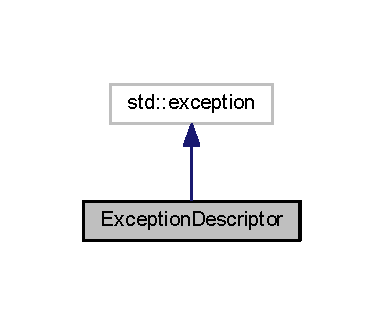
\includegraphics[width=184pt]{class_exception_descriptor__inherit__graph}
\end{center}
\end{figure}


Collaboration diagram for Exception\-Descriptor\-:
\nopagebreak
\begin{figure}[H]
\begin{center}
\leavevmode
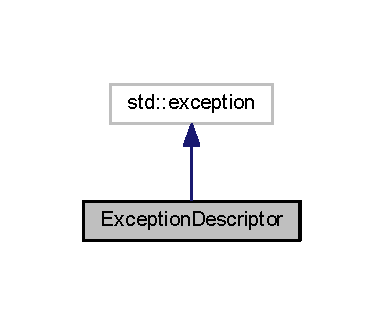
\includegraphics[width=184pt]{class_exception_descriptor__coll__graph}
\end{center}
\end{figure}
\subsubsection*{Public Member Functions}
\begin{DoxyCompactItemize}
\item 
\hyperlink{group___core_abd7c2af705e7d6d9f2310fa676e1a74c}{Exception\-Descriptor} (const std\-::string \&error, const std\-::string \&file\-Name, const std\-::string \&func\-Name, int line, bool is\-Error=true)  throw ()
\begin{DoxyCompactList}\small\item\em Constructor. \end{DoxyCompactList}\item 
\hyperlink{group___core_a0d0840e46e4874851fcb4cb74767eeb3}{Exception\-Descriptor} (const \hyperlink{group___core_class_exception_descriptor}{Exception\-Descriptor} \&e)  throw ()
\begin{DoxyCompactList}\small\item\em Copy constructor. \end{DoxyCompactList}\item 
\hyperlink{group___core_accf5a093a12051f43c439aa5435b581a}{$\sim$\-Exception\-Descriptor} (void)  throw ()
\begin{DoxyCompactList}\small\item\em Destructor. \end{DoxyCompactList}\item 
void \hyperlink{group___core_a9796603ac150535b2986f307bb4e6f1b}{Trace\-Error} (void)  throw ()
\begin{DoxyCompactList}\small\item\em Write the exception description to stderr. \end{DoxyCompactList}\item 
const char $\ast$ \hyperlink{group___core_a9976a798b37f87e8e60d893e0ccaa86c}{what} (void) const   throw ()
\begin{DoxyCompactList}\small\item\em std\-::exception\-::what() \end{DoxyCompactList}\end{DoxyCompactItemize}
\subsubsection*{Private Attributes}
\begin{DoxyCompactItemize}
\item 
std\-::string \hyperlink{group___core_a9a0ee9381ed48d3d315a9e091be1d817}{error\-\_\-}
\begin{DoxyCompactList}\small\item\em Error message. \end{DoxyCompactList}\item 
std\-::string \hyperlink{group___core_a28d43a19c103c7622e5fb225d9ac81bc}{file\-Name\-\_\-}
\begin{DoxyCompactList}\small\item\em Name of the file. \end{DoxyCompactList}\item 
std\-::string \hyperlink{group___core_a338c02c76b2631e1948b3d15dd256c5f}{func\-Name\-\_\-}
\begin{DoxyCompactList}\small\item\em Name of the function. \end{DoxyCompactList}\item 
bool \hyperlink{group___core_ae59cb81febf52e97aac91bcc5006c4f0}{is\-Error\-\_\-}
\begin{DoxyCompactList}\small\item\em Error or abnormal operation. \end{DoxyCompactList}\item 
int \hyperlink{group___core_aa6b8d6a6cadfe9e645409bb1ab8fd788}{line\-\_\-}
\begin{DoxyCompactList}\small\item\em Line number. \end{DoxyCompactList}\end{DoxyCompactItemize}


\paragraph{Constructor \& Destructor Documentation}
\hypertarget{group___core_abd7c2af705e7d6d9f2310fa676e1a74c}{\index{Exception\-Descriptor@{Exception\-Descriptor}!Exception\-Descriptor@{Exception\-Descriptor}}
\index{Exception\-Descriptor@{Exception\-Descriptor}!ExceptionDescriptor@{Exception\-Descriptor}}
\subparagraph[{Exception\-Descriptor}]{\setlength{\rightskip}{0pt plus 5cm}Exception\-Descriptor\-::\-Exception\-Descriptor (
\begin{DoxyParamCaption}
\item[{const std\-::string \&}]{error, }
\item[{const std\-::string \&}]{file\-Name, }
\item[{const std\-::string \&}]{func\-Name, }
\item[{int}]{line, }
\item[{bool}]{is\-Error = {\ttfamily true}}
\end{DoxyParamCaption}
)  throw ()}}\label{group___core_abd7c2af705e7d6d9f2310fa676e1a74c}


Constructor. 


\begin{DoxyParams}{Parameters}
{\em error} & Error message. \\
\hline
{\em file\-Name} & Name of the file in which the exception was raised. \\
\hline
{\em func\-Name} & Name of the function in which the exception was raised. \\
\hline
{\em line} & Number of line on which the exception was raised. \\
\hline
{\em is\-Error} & Error or abnormal operation.\\
\hline
\end{DoxyParams}
Should be used through the macro New\-Error(message) or New\-Warning(message). \hypertarget{group___core_a0d0840e46e4874851fcb4cb74767eeb3}{\index{Exception\-Descriptor@{Exception\-Descriptor}!Exception\-Descriptor@{Exception\-Descriptor}}
\index{Exception\-Descriptor@{Exception\-Descriptor}!ExceptionDescriptor@{Exception\-Descriptor}}
\subparagraph[{Exception\-Descriptor}]{\setlength{\rightskip}{0pt plus 5cm}Exception\-Descriptor\-::\-Exception\-Descriptor (
\begin{DoxyParamCaption}
\item[{const {\bf Exception\-Descriptor} \&}]{e}
\end{DoxyParamCaption}
)  throw ()}}\label{group___core_a0d0840e46e4874851fcb4cb74767eeb3}


Copy constructor. 


\begin{DoxyParams}{Parameters}
{\em e} & Another \hyperlink{group___core_class_exception_descriptor}{Exception\-Descriptor}. \\
\hline
\end{DoxyParams}
\hypertarget{group___core_accf5a093a12051f43c439aa5435b581a}{\index{Exception\-Descriptor@{Exception\-Descriptor}!$\sim$\-Exception\-Descriptor@{$\sim$\-Exception\-Descriptor}}
\index{$\sim$\-Exception\-Descriptor@{$\sim$\-Exception\-Descriptor}!ExceptionDescriptor@{Exception\-Descriptor}}
\subparagraph[{$\sim$\-Exception\-Descriptor}]{\setlength{\rightskip}{0pt plus 5cm}Exception\-Descriptor\-::$\sim$\-Exception\-Descriptor (
\begin{DoxyParamCaption}
\item[{void}]{}
\end{DoxyParamCaption}
)  throw ()}}\label{group___core_accf5a093a12051f43c439aa5435b581a}


Destructor. 



\paragraph{Member Function Documentation}
\hypertarget{group___core_a9796603ac150535b2986f307bb4e6f1b}{\index{Exception\-Descriptor@{Exception\-Descriptor}!Trace\-Error@{Trace\-Error}}
\index{Trace\-Error@{Trace\-Error}!ExceptionDescriptor@{Exception\-Descriptor}}
\subparagraph[{Trace\-Error}]{\setlength{\rightskip}{0pt plus 5cm}void Exception\-Descriptor\-::\-Trace\-Error (
\begin{DoxyParamCaption}
\item[{void}]{}
\end{DoxyParamCaption}
)  throw ()}}\label{group___core_a9796603ac150535b2986f307bb4e6f1b}


Write the exception description to stderr. 



Here is the caller graph for this function\-:
\nopagebreak
\begin{figure}[H]
\begin{center}
\leavevmode
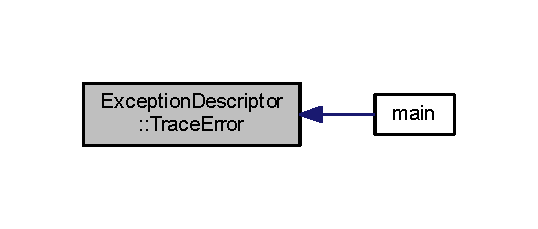
\includegraphics[width=258pt]{group___core_a9796603ac150535b2986f307bb4e6f1b_icgraph}
\end{center}
\end{figure}


\hypertarget{group___core_a9976a798b37f87e8e60d893e0ccaa86c}{\index{Exception\-Descriptor@{Exception\-Descriptor}!what@{what}}
\index{what@{what}!ExceptionDescriptor@{Exception\-Descriptor}}
\subparagraph[{what}]{\setlength{\rightskip}{0pt plus 5cm}const char $\ast$ Exception\-Descriptor\-::what (
\begin{DoxyParamCaption}
\item[{void}]{}
\end{DoxyParamCaption}
) const  throw ()}}\label{group___core_a9976a798b37f87e8e60d893e0ccaa86c}


std\-::exception\-::what() 



\paragraph{Member Data Documentation}
\hypertarget{group___core_a9a0ee9381ed48d3d315a9e091be1d817}{\index{Exception\-Descriptor@{Exception\-Descriptor}!error\-\_\-@{error\-\_\-}}
\index{error\-\_\-@{error\-\_\-}!ExceptionDescriptor@{Exception\-Descriptor}}
\subparagraph[{error\-\_\-}]{\setlength{\rightskip}{0pt plus 5cm}std\-::string Exception\-Descriptor\-::error\-\_\-\hspace{0.3cm}{\ttfamily [private]}}}\label{group___core_a9a0ee9381ed48d3d315a9e091be1d817}


Error message. 

\hypertarget{group___core_a28d43a19c103c7622e5fb225d9ac81bc}{\index{Exception\-Descriptor@{Exception\-Descriptor}!file\-Name\-\_\-@{file\-Name\-\_\-}}
\index{file\-Name\-\_\-@{file\-Name\-\_\-}!ExceptionDescriptor@{Exception\-Descriptor}}
\subparagraph[{file\-Name\-\_\-}]{\setlength{\rightskip}{0pt plus 5cm}std\-::string Exception\-Descriptor\-::file\-Name\-\_\-\hspace{0.3cm}{\ttfamily [private]}}}\label{group___core_a28d43a19c103c7622e5fb225d9ac81bc}


Name of the file. 

\hypertarget{group___core_a338c02c76b2631e1948b3d15dd256c5f}{\index{Exception\-Descriptor@{Exception\-Descriptor}!func\-Name\-\_\-@{func\-Name\-\_\-}}
\index{func\-Name\-\_\-@{func\-Name\-\_\-}!ExceptionDescriptor@{Exception\-Descriptor}}
\subparagraph[{func\-Name\-\_\-}]{\setlength{\rightskip}{0pt plus 5cm}std\-::string Exception\-Descriptor\-::func\-Name\-\_\-\hspace{0.3cm}{\ttfamily [private]}}}\label{group___core_a338c02c76b2631e1948b3d15dd256c5f}


Name of the function. 

\hypertarget{group___core_ae59cb81febf52e97aac91bcc5006c4f0}{\index{Exception\-Descriptor@{Exception\-Descriptor}!is\-Error\-\_\-@{is\-Error\-\_\-}}
\index{is\-Error\-\_\-@{is\-Error\-\_\-}!ExceptionDescriptor@{Exception\-Descriptor}}
\subparagraph[{is\-Error\-\_\-}]{\setlength{\rightskip}{0pt plus 5cm}bool Exception\-Descriptor\-::is\-Error\-\_\-\hspace{0.3cm}{\ttfamily [private]}}}\label{group___core_ae59cb81febf52e97aac91bcc5006c4f0}


Error or abnormal operation. 

\hypertarget{group___core_aa6b8d6a6cadfe9e645409bb1ab8fd788}{\index{Exception\-Descriptor@{Exception\-Descriptor}!line\-\_\-@{line\-\_\-}}
\index{line\-\_\-@{line\-\_\-}!ExceptionDescriptor@{Exception\-Descriptor}}
\subparagraph[{line\-\_\-}]{\setlength{\rightskip}{0pt plus 5cm}int Exception\-Descriptor\-::line\-\_\-\hspace{0.3cm}{\ttfamily [private]}}}\label{group___core_aa6b8d6a6cadfe9e645409bb1ab8fd788}


Line number. 

\index{Image\-Frame@{Image\-Frame}}\label{class_image_frame}
\hypertarget{group___core_class_image_frame}{}
\subsubsection{class Image\-Frame}
Image frame wrapper class. 

Gets image frames as cv\-::\-Mat objects. \subsubsection*{Public Member Functions}
\begin{DoxyCompactItemize}
\item 
\hyperlink{group___core_a117419148b5bcc26cc145d3f2f186bad}{Image\-Frame} (int camera\-Id)
\begin{DoxyCompactList}\small\item\em Constructor. \end{DoxyCompactList}\item 
\hyperlink{group___core_a59c1d9b9e30400514172b549b5f087d9}{Image\-Frame} (const std\-::string \&image\-Name)
\begin{DoxyCompactList}\small\item\em Constructor. \end{DoxyCompactList}\item 
\hyperlink{group___core_a2f365f54366e61d0fffe41a2e24ba570}{$\sim$\-Image\-Frame} (void)
\begin{DoxyCompactList}\small\item\em Destructor. \end{DoxyCompactList}\item 
const cv\-::\-Mat \& \hyperlink{group___core_a886d65831c708b65ba5596aab1aca438}{Get\-Frame} (void)
\begin{DoxyCompactList}\small\item\em Gets a frame from somewhere. \end{DoxyCompactList}\end{DoxyCompactItemize}
\subsubsection*{Private Attributes}
\begin{DoxyCompactItemize}
\item 
cv\-::\-Video\-Capture \hyperlink{group___core_a1f8ba0c6c7f724a41f5f5fef19bfe035}{cap\-\_\-}
\begin{DoxyCompactList}\small\item\em Temporary capture for getting frame. \end{DoxyCompactList}\item 
cv\-::\-Mat \hyperlink{group___core_a6aaede1e96c67711280696df991b4508}{frame\-\_\-}
\begin{DoxyCompactList}\small\item\em Loaded or captured image. \end{DoxyCompactList}\end{DoxyCompactItemize}


\paragraph{Constructor \& Destructor Documentation}
\hypertarget{group___core_a117419148b5bcc26cc145d3f2f186bad}{\index{Image\-Frame@{Image\-Frame}!Image\-Frame@{Image\-Frame}}
\index{Image\-Frame@{Image\-Frame}!ImageFrame@{Image\-Frame}}
\subparagraph[{Image\-Frame}]{\setlength{\rightskip}{0pt plus 5cm}Image\-Frame\-::\-Image\-Frame (
\begin{DoxyParamCaption}
\item[{int}]{camera\-Id = {\ttfamily 0}}
\end{DoxyParamCaption}
)}}\label{group___core_a117419148b5bcc26cc145d3f2f186bad}


Constructor. 


\begin{DoxyParams}{Parameters}
{\em camera\-Id} & I\-D of the camera. \\
\hline
\end{DoxyParams}
\hypertarget{group___core_a59c1d9b9e30400514172b549b5f087d9}{\index{Image\-Frame@{Image\-Frame}!Image\-Frame@{Image\-Frame}}
\index{Image\-Frame@{Image\-Frame}!ImageFrame@{Image\-Frame}}
\subparagraph[{Image\-Frame}]{\setlength{\rightskip}{0pt plus 5cm}Image\-Frame\-::\-Image\-Frame (
\begin{DoxyParamCaption}
\item[{const std\-::string \&}]{image\-Name}
\end{DoxyParamCaption}
)}}\label{group___core_a59c1d9b9e30400514172b549b5f087d9}


Constructor. 


\begin{DoxyParams}{Parameters}
{\em image\-Name} & Name of the image, which from the features will be extracted. \\
\hline
\end{DoxyParams}
\hypertarget{group___core_a2f365f54366e61d0fffe41a2e24ba570}{\index{Image\-Frame@{Image\-Frame}!$\sim$\-Image\-Frame@{$\sim$\-Image\-Frame}}
\index{$\sim$\-Image\-Frame@{$\sim$\-Image\-Frame}!ImageFrame@{Image\-Frame}}
\subparagraph[{$\sim$\-Image\-Frame}]{\setlength{\rightskip}{0pt plus 5cm}Image\-Frame\-::$\sim$\-Image\-Frame (
\begin{DoxyParamCaption}
\item[{void}]{}
\end{DoxyParamCaption}
)}}\label{group___core_a2f365f54366e61d0fffe41a2e24ba570}


Destructor. 



\paragraph{Member Function Documentation}
\hypertarget{group___core_a886d65831c708b65ba5596aab1aca438}{\index{Image\-Frame@{Image\-Frame}!Get\-Frame@{Get\-Frame}}
\index{Get\-Frame@{Get\-Frame}!ImageFrame@{Image\-Frame}}
\subparagraph[{Get\-Frame}]{\setlength{\rightskip}{0pt plus 5cm}const Mat \& Image\-Frame\-::\-Get\-Frame (
\begin{DoxyParamCaption}
\item[{void}]{}
\end{DoxyParamCaption}
)}}\label{group___core_a886d65831c708b65ba5596aab1aca438}


Gets a frame from somewhere. 

\begin{DoxyReturn}{Returns}
frame Output argument for the frame. 
\end{DoxyReturn}


Here is the caller graph for this function\-:
\nopagebreak
\begin{figure}[H]
\begin{center}
\leavevmode
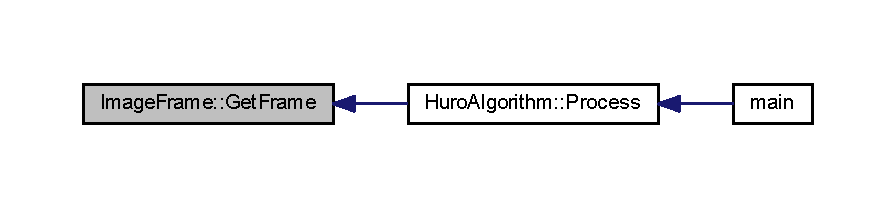
\includegraphics[width=350pt]{group___core_a886d65831c708b65ba5596aab1aca438_icgraph}
\end{center}
\end{figure}




\paragraph{Member Data Documentation}
\hypertarget{group___core_a1f8ba0c6c7f724a41f5f5fef19bfe035}{\index{Image\-Frame@{Image\-Frame}!cap\-\_\-@{cap\-\_\-}}
\index{cap\-\_\-@{cap\-\_\-}!ImageFrame@{Image\-Frame}}
\subparagraph[{cap\-\_\-}]{\setlength{\rightskip}{0pt plus 5cm}cv\-::\-Video\-Capture Image\-Frame\-::cap\-\_\-\hspace{0.3cm}{\ttfamily [private]}}}\label{group___core_a1f8ba0c6c7f724a41f5f5fef19bfe035}


Temporary capture for getting frame. 

\hypertarget{group___core_a6aaede1e96c67711280696df991b4508}{\index{Image\-Frame@{Image\-Frame}!frame\-\_\-@{frame\-\_\-}}
\index{frame\-\_\-@{frame\-\_\-}!ImageFrame@{Image\-Frame}}
\subparagraph[{frame\-\_\-}]{\setlength{\rightskip}{0pt plus 5cm}cv\-::\-Mat Image\-Frame\-::frame\-\_\-\hspace{0.3cm}{\ttfamily [private]}}}\label{group___core_a6aaede1e96c67711280696df991b4508}


Loaded or captured image. 

\index{Local\-Settings@{Local\-Settings}}\label{class_local_settings}
\hypertarget{group___core_class_local_settings}{}
\subsubsection{class Local\-Settings}
Singleton settings manager class. 

Contains the paths of X\-M\-Ls and video files. \subsubsection*{Public Member Functions}
\begin{DoxyCompactItemize}
\item 
std\-::string \hyperlink{group___core_aaa62a3ad7984bb9b41d874a432f80eb5}{Get\-Data\-Directory} (void) const 
\begin{DoxyCompactList}\small\item\em Data directory getter. \end{DoxyCompactList}\item 
std\-::string \hyperlink{group___core_abbaecb0ce832b89c7851af0d7931cf89}{Get\-Image\-Directory} (void) const 
\begin{DoxyCompactList}\small\item\em Image directory getter. \end{DoxyCompactList}\item 
std\-::string \hyperlink{group___core_a2ab12f5691406aa7ad21140fd3a94f27}{Get\-Process\-Xml\-File\-Name} (void) const 
\begin{DoxyCompactList}\small\item\em Process xml filename getter. \end{DoxyCompactList}\item 
std\-::string \hyperlink{group___core_adfd6c887c7c35c76bce216dda592170d}{Get\-Settings\-Directory} (void) const 
\begin{DoxyCompactList}\small\item\em Settings directory getter. \end{DoxyCompactList}\end{DoxyCompactItemize}
\subsubsection*{Static Public Member Functions}
\begin{DoxyCompactItemize}
\item 
static \hyperlink{group___core_class_local_settings}{Local\-Settings} $\ast$ \hyperlink{group___core_a80f6e158e8c61b70fd4efec296e28310}{Get\-Instance} (void)
\begin{DoxyCompactList}\small\item\em Instance getter. \end{DoxyCompactList}\end{DoxyCompactItemize}
\subsubsection*{Private Member Functions}
\begin{DoxyCompactItemize}
\item 
\hyperlink{group___core_a70ef22059fb84a1a64120f3122db615e}{Local\-Settings} (void)
\begin{DoxyCompactList}\small\item\em Constructor. \end{DoxyCompactList}\item 
\hyperlink{group___core_a043074a18b94b6c572e31feb2d283926}{$\sim$\-Local\-Settings} (void)
\begin{DoxyCompactList}\small\item\em Destructor. \end{DoxyCompactList}\end{DoxyCompactItemize}
\subsubsection*{Private Attributes}
\begin{DoxyCompactItemize}
\item 
std\-::string \hyperlink{group___core_a7cddf57927891a603552ca37a8839f22}{data\-Directory\-\_\-}
\begin{DoxyCompactList}\small\item\em Data directory root. \end{DoxyCompactList}\item 
std\-::string \hyperlink{group___core_aef55a56deb4853e3c7c2d17f87a65be7}{image\-Directory\-\_\-}
\begin{DoxyCompactList}\small\item\em Image directory root. \end{DoxyCompactList}\item 
std\-::string \hyperlink{group___core_a19de001426c0ff8e8d4284202b929b08}{process\-Xml\-File\-Name\-\_\-}
\begin{DoxyCompactList}\small\item\em The configuration file. \end{DoxyCompactList}\item 
std\-::string \hyperlink{group___core_af27f60deac73d6236070b4b78ed2fcbf}{settings\-Directory\-\_\-}
\begin{DoxyCompactList}\small\item\em Settings directory root. \end{DoxyCompactList}\end{DoxyCompactItemize}


\paragraph{Constructor \& Destructor Documentation}
\hypertarget{group___core_a70ef22059fb84a1a64120f3122db615e}{\index{Local\-Settings@{Local\-Settings}!Local\-Settings@{Local\-Settings}}
\index{Local\-Settings@{Local\-Settings}!LocalSettings@{Local\-Settings}}
\subparagraph[{Local\-Settings}]{\setlength{\rightskip}{0pt plus 5cm}Local\-Settings\-::\-Local\-Settings (
\begin{DoxyParamCaption}
\item[{void}]{}
\end{DoxyParamCaption}
)\hspace{0.3cm}{\ttfamily [private]}}}\label{group___core_a70ef22059fb84a1a64120f3122db615e}


Constructor. 

\hypertarget{group___core_a043074a18b94b6c572e31feb2d283926}{\index{Local\-Settings@{Local\-Settings}!$\sim$\-Local\-Settings@{$\sim$\-Local\-Settings}}
\index{$\sim$\-Local\-Settings@{$\sim$\-Local\-Settings}!LocalSettings@{Local\-Settings}}
\subparagraph[{$\sim$\-Local\-Settings}]{\setlength{\rightskip}{0pt plus 5cm}Local\-Settings\-::$\sim$\-Local\-Settings (
\begin{DoxyParamCaption}
\item[{void}]{}
\end{DoxyParamCaption}
)\hspace{0.3cm}{\ttfamily [private]}}}\label{group___core_a043074a18b94b6c572e31feb2d283926}


Destructor. 



\paragraph{Member Function Documentation}
\hypertarget{group___core_aaa62a3ad7984bb9b41d874a432f80eb5}{\index{Local\-Settings@{Local\-Settings}!Get\-Data\-Directory@{Get\-Data\-Directory}}
\index{Get\-Data\-Directory@{Get\-Data\-Directory}!LocalSettings@{Local\-Settings}}
\subparagraph[{Get\-Data\-Directory}]{\setlength{\rightskip}{0pt plus 5cm}string Local\-Settings\-::\-Get\-Data\-Directory (
\begin{DoxyParamCaption}
\item[{void}]{}
\end{DoxyParamCaption}
) const}}\label{group___core_aaa62a3ad7984bb9b41d874a432f80eb5}


Data directory getter. 

\begin{DoxyReturn}{Returns}
Data directory root. 
\end{DoxyReturn}
\hypertarget{group___core_abbaecb0ce832b89c7851af0d7931cf89}{\index{Local\-Settings@{Local\-Settings}!Get\-Image\-Directory@{Get\-Image\-Directory}}
\index{Get\-Image\-Directory@{Get\-Image\-Directory}!LocalSettings@{Local\-Settings}}
\subparagraph[{Get\-Image\-Directory}]{\setlength{\rightskip}{0pt plus 5cm}string Local\-Settings\-::\-Get\-Image\-Directory (
\begin{DoxyParamCaption}
\item[{void}]{}
\end{DoxyParamCaption}
) const}}\label{group___core_abbaecb0ce832b89c7851af0d7931cf89}


Image directory getter. 

\begin{DoxyReturn}{Returns}
Settings directory root. 
\end{DoxyReturn}
\hypertarget{group___core_a80f6e158e8c61b70fd4efec296e28310}{\index{Local\-Settings@{Local\-Settings}!Get\-Instance@{Get\-Instance}}
\index{Get\-Instance@{Get\-Instance}!LocalSettings@{Local\-Settings}}
\subparagraph[{Get\-Instance}]{\setlength{\rightskip}{0pt plus 5cm}{\bf Local\-Settings} $\ast$ Local\-Settings\-::\-Get\-Instance (
\begin{DoxyParamCaption}
\item[{void}]{}
\end{DoxyParamCaption}
)\hspace{0.3cm}{\ttfamily [static]}}}\label{group___core_a80f6e158e8c61b70fd4efec296e28310}


Instance getter. 

\begin{DoxyReturn}{Returns}
The instance. 
\end{DoxyReturn}
\hypertarget{group___core_a2ab12f5691406aa7ad21140fd3a94f27}{\index{Local\-Settings@{Local\-Settings}!Get\-Process\-Xml\-File\-Name@{Get\-Process\-Xml\-File\-Name}}
\index{Get\-Process\-Xml\-File\-Name@{Get\-Process\-Xml\-File\-Name}!LocalSettings@{Local\-Settings}}
\subparagraph[{Get\-Process\-Xml\-File\-Name}]{\setlength{\rightskip}{0pt plus 5cm}string Local\-Settings\-::\-Get\-Process\-Xml\-File\-Name (
\begin{DoxyParamCaption}
\item[{void}]{}
\end{DoxyParamCaption}
) const}}\label{group___core_a2ab12f5691406aa7ad21140fd3a94f27}


Process xml filename getter. 

\begin{DoxyReturn}{Returns}
Settings directory root. 
\end{DoxyReturn}
\hypertarget{group___core_adfd6c887c7c35c76bce216dda592170d}{\index{Local\-Settings@{Local\-Settings}!Get\-Settings\-Directory@{Get\-Settings\-Directory}}
\index{Get\-Settings\-Directory@{Get\-Settings\-Directory}!LocalSettings@{Local\-Settings}}
\subparagraph[{Get\-Settings\-Directory}]{\setlength{\rightskip}{0pt plus 5cm}string Local\-Settings\-::\-Get\-Settings\-Directory (
\begin{DoxyParamCaption}
\item[{void}]{}
\end{DoxyParamCaption}
) const}}\label{group___core_adfd6c887c7c35c76bce216dda592170d}


Settings directory getter. 

\begin{DoxyReturn}{Returns}
Settings directory root. 
\end{DoxyReturn}


\paragraph{Member Data Documentation}
\hypertarget{group___core_a7cddf57927891a603552ca37a8839f22}{\index{Local\-Settings@{Local\-Settings}!data\-Directory\-\_\-@{data\-Directory\-\_\-}}
\index{data\-Directory\-\_\-@{data\-Directory\-\_\-}!LocalSettings@{Local\-Settings}}
\subparagraph[{data\-Directory\-\_\-}]{\setlength{\rightskip}{0pt plus 5cm}std\-::string Local\-Settings\-::data\-Directory\-\_\-\hspace{0.3cm}{\ttfamily [private]}}}\label{group___core_a7cddf57927891a603552ca37a8839f22}


Data directory root. 

\hypertarget{group___core_aef55a56deb4853e3c7c2d17f87a65be7}{\index{Local\-Settings@{Local\-Settings}!image\-Directory\-\_\-@{image\-Directory\-\_\-}}
\index{image\-Directory\-\_\-@{image\-Directory\-\_\-}!LocalSettings@{Local\-Settings}}
\subparagraph[{image\-Directory\-\_\-}]{\setlength{\rightskip}{0pt plus 5cm}std\-::string Local\-Settings\-::image\-Directory\-\_\-\hspace{0.3cm}{\ttfamily [private]}}}\label{group___core_aef55a56deb4853e3c7c2d17f87a65be7}


Image directory root. 

\hypertarget{group___core_a19de001426c0ff8e8d4284202b929b08}{\index{Local\-Settings@{Local\-Settings}!process\-Xml\-File\-Name\-\_\-@{process\-Xml\-File\-Name\-\_\-}}
\index{process\-Xml\-File\-Name\-\_\-@{process\-Xml\-File\-Name\-\_\-}!LocalSettings@{Local\-Settings}}
\subparagraph[{process\-Xml\-File\-Name\-\_\-}]{\setlength{\rightskip}{0pt plus 5cm}std\-::string Local\-Settings\-::process\-Xml\-File\-Name\-\_\-\hspace{0.3cm}{\ttfamily [private]}}}\label{group___core_a19de001426c0ff8e8d4284202b929b08}


The configuration file. 

\hypertarget{group___core_af27f60deac73d6236070b4b78ed2fcbf}{\index{Local\-Settings@{Local\-Settings}!settings\-Directory\-\_\-@{settings\-Directory\-\_\-}}
\index{settings\-Directory\-\_\-@{settings\-Directory\-\_\-}!LocalSettings@{Local\-Settings}}
\subparagraph[{settings\-Directory\-\_\-}]{\setlength{\rightskip}{0pt plus 5cm}std\-::string Local\-Settings\-::settings\-Directory\-\_\-\hspace{0.3cm}{\ttfamily [private]}}}\label{group___core_af27f60deac73d6236070b4b78ed2fcbf}


Settings directory root. 

\index{Mutex@{Mutex}}\label{class_mutex}
\hypertarget{group___core_class_mutex}{}
\subsubsection{class Mutex}
A synchronization primitive that can also be used for interprocess synchronization. 

When two or more threads need to access a shared resource at the same time, the system needs a synchronization mechanism to ensure that only one thread at a time uses the resource. \hyperlink{group___core_class_mutex}{Mutex} is a synchronization primitive that grants exclusive access to the shared resource to only one thread. \subsubsection*{Public Member Functions}
\begin{DoxyCompactItemize}
\item 
\hyperlink{group___core_a00b2ff557451955a905ecdca2855389b}{Mutex} (void)
\begin{DoxyCompactList}\small\item\em Constructor. \end{DoxyCompactList}\item 
\hyperlink{group___core_a115e8bae072b7d0767f75bc3369d521d}{$\sim$\-Mutex} (void)
\begin{DoxyCompactList}\small\item\em Destructor. \end{DoxyCompactList}\item 
void \hyperlink{group___core_a1726d7244983f7be74fcfa9cfb63745f}{Lock} (void)
\begin{DoxyCompactList}\small\item\em Blocks the current thread. \end{DoxyCompactList}\item 
void \hyperlink{group___core_a03150e8fa423f7e042661d350d238b84}{Unlock} (void)
\begin{DoxyCompactList}\small\item\em Unblocks the current thread. \end{DoxyCompactList}\end{DoxyCompactItemize}
\subsubsection*{Private Attributes}
\begin{DoxyCompactItemize}
\item 
pthread\-\_\-mutex\-\_\-t \hyperlink{group___core_a0f845aa1acc03f39fd84612c91050f27}{mutex\-\_\-}
\begin{DoxyCompactList}\small\item\em Inner mutex object. \end{DoxyCompactList}\end{DoxyCompactItemize}


\paragraph{Constructor \& Destructor Documentation}
\hypertarget{group___core_a00b2ff557451955a905ecdca2855389b}{\index{Mutex@{Mutex}!Mutex@{Mutex}}
\index{Mutex@{Mutex}!Mutex@{Mutex}}
\subparagraph[{Mutex}]{\setlength{\rightskip}{0pt plus 5cm}Mutex\-::\-Mutex (
\begin{DoxyParamCaption}
\item[{void}]{}
\end{DoxyParamCaption}
)}}\label{group___core_a00b2ff557451955a905ecdca2855389b}


Constructor. 

\hypertarget{group___core_a115e8bae072b7d0767f75bc3369d521d}{\index{Mutex@{Mutex}!$\sim$\-Mutex@{$\sim$\-Mutex}}
\index{$\sim$\-Mutex@{$\sim$\-Mutex}!Mutex@{Mutex}}
\subparagraph[{$\sim$\-Mutex}]{\setlength{\rightskip}{0pt plus 5cm}Mutex\-::$\sim$\-Mutex (
\begin{DoxyParamCaption}
\item[{void}]{}
\end{DoxyParamCaption}
)}}\label{group___core_a115e8bae072b7d0767f75bc3369d521d}


Destructor. 



\paragraph{Member Function Documentation}
\hypertarget{group___core_a1726d7244983f7be74fcfa9cfb63745f}{\index{Mutex@{Mutex}!Lock@{Lock}}
\index{Lock@{Lock}!Mutex@{Mutex}}
\subparagraph[{Lock}]{\setlength{\rightskip}{0pt plus 5cm}void Mutex\-::\-Lock (
\begin{DoxyParamCaption}
\item[{void}]{}
\end{DoxyParamCaption}
)}}\label{group___core_a1726d7244983f7be74fcfa9cfb63745f}


Blocks the current thread. 

\hypertarget{group___core_a03150e8fa423f7e042661d350d238b84}{\index{Mutex@{Mutex}!Unlock@{Unlock}}
\index{Unlock@{Unlock}!Mutex@{Mutex}}
\subparagraph[{Unlock}]{\setlength{\rightskip}{0pt plus 5cm}void Mutex\-::\-Unlock (
\begin{DoxyParamCaption}
\item[{void}]{}
\end{DoxyParamCaption}
)}}\label{group___core_a03150e8fa423f7e042661d350d238b84}


Unblocks the current thread. 



\paragraph{Member Data Documentation}
\hypertarget{group___core_a0f845aa1acc03f39fd84612c91050f27}{\index{Mutex@{Mutex}!mutex\-\_\-@{mutex\-\_\-}}
\index{mutex\-\_\-@{mutex\-\_\-}!Mutex@{Mutex}}
\subparagraph[{mutex\-\_\-}]{\setlength{\rightskip}{0pt plus 5cm}pthread\-\_\-mutex\-\_\-t Mutex\-::mutex\-\_\-\hspace{0.3cm}{\ttfamily [private]}}}\label{group___core_a0f845aa1acc03f39fd84612c91050f27}


Inner mutex object. 

\index{Runnable@{Runnable}}\label{class_runnable}
\hypertarget{group___core_class_runnable}{}
\subsubsection{class Runnable}
Abstract interface for runnable objects. \subsubsection*{Public Member Functions}
\begin{DoxyCompactItemize}
\item 
virtual \hyperlink{group___core_a12fa87f2064fa19c66c23c6dcd7387f6}{$\sim$\-Runnable} (void)=0
\begin{DoxyCompactList}\small\item\em Destructor. \end{DoxyCompactList}\item 
virtual void $\ast$ \hyperlink{group___core_a60c67afa6b8045533fa9ee5243288067}{Run} (void)=0
\begin{DoxyCompactList}\small\item\em Pure virtual thread main. \end{DoxyCompactList}\end{DoxyCompactItemize}


\paragraph{Constructor \& Destructor Documentation}
\hypertarget{group___core_a12fa87f2064fa19c66c23c6dcd7387f6}{\index{Runnable@{Runnable}!$\sim$\-Runnable@{$\sim$\-Runnable}}
\index{$\sim$\-Runnable@{$\sim$\-Runnable}!Runnable@{Runnable}}
\subparagraph[{$\sim$\-Runnable}]{\setlength{\rightskip}{0pt plus 5cm}Runnable\-::$\sim$\-Runnable (
\begin{DoxyParamCaption}
\item[{void}]{}
\end{DoxyParamCaption}
)\hspace{0.3cm}{\ttfamily [pure virtual]}}}\label{group___core_a12fa87f2064fa19c66c23c6dcd7387f6}


Destructor. 



\paragraph{Member Function Documentation}
\hypertarget{group___core_a60c67afa6b8045533fa9ee5243288067}{\index{Runnable@{Runnable}!Run@{Run}}
\index{Run@{Run}!Runnable@{Runnable}}
\subparagraph[{Run}]{\setlength{\rightskip}{0pt plus 5cm}virtual void$\ast$ Runnable\-::\-Run (
\begin{DoxyParamCaption}
\item[{void}]{}
\end{DoxyParamCaption}
)\hspace{0.3cm}{\ttfamily [pure virtual]}}}\label{group___core_a60c67afa6b8045533fa9ee5243288067}


Pure virtual thread main. 

\index{Thread@{Thread}}\label{class_thread}
\hypertarget{group___core_class_thread}{}
\subsubsection{class Thread}
Abstract class for handling threads. 

\hyperlink{group___core_class_runnable}{Runnable} classes can be derived from this class.

Threads can be started and stopped with the \hyperlink{group___core_a2b42f82341afd2747ea093b6ac8b91cb}{Start()} and \hyperlink{group___core_a8f33f7750321d5df9188033e7e3e300d}{Join()} methods respectively. The new thread will enter the implemented \hyperlink{group___core_ae46cda1b57e998b239a8b9710b0712e2}{Run()} method. 

Inheritance diagram for Thread\-:\nopagebreak
\begin{figure}[H]
\begin{center}
\leavevmode
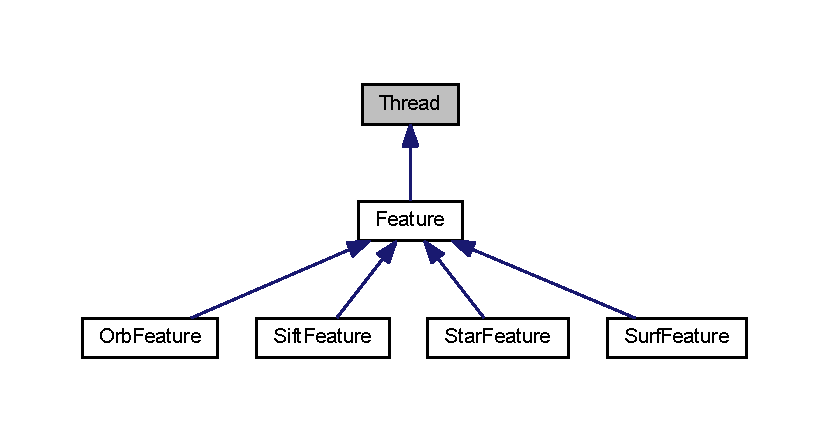
\includegraphics[width=350pt]{class_thread__inherit__graph}
\end{center}
\end{figure}
\subsubsection*{Public Member Functions}
\begin{DoxyCompactItemize}
\item 
\hyperlink{group___core_a027b9eb38e4d59c076501b305b42f575}{Thread} (std\-::auto\-\_\-ptr$<$ \hyperlink{group___core_class_runnable}{Runnable} $>$ run, bool is\-Detached=false)
\begin{DoxyCompactList}\small\item\em Constructor. \end{DoxyCompactList}\item 
\hyperlink{group___core_a403714feecd93ac10c101a47b7649204}{Thread} (bool is\-Detached=false)
\begin{DoxyCompactList}\small\item\em Constructor. \end{DoxyCompactList}\item 
virtual \hyperlink{group___core_af1e25588ebe47a2a6d79ef8c686a992b}{$\sim$\-Thread} (void)
\begin{DoxyCompactList}\small\item\em Destructor. \end{DoxyCompactList}\item 
void $\ast$ \hyperlink{group___core_a8f33f7750321d5df9188033e7e3e300d}{Join} (void)
\item 
void \hyperlink{group___core_a2b42f82341afd2747ea093b6ac8b91cb}{Start} (void)
\begin{DoxyCompactList}\small\item\em Starts the thread. \end{DoxyCompactList}\end{DoxyCompactItemize}
\subsubsection*{Private Member Functions}
\begin{DoxyCompactItemize}
\item 
virtual void $\ast$ \hyperlink{group___core_ae46cda1b57e998b239a8b9710b0712e2}{Run} (void)=0
\begin{DoxyCompactList}\small\item\em Pure virtual thread main. \end{DoxyCompactList}\item 
void \hyperlink{group___core_ac32823199dc71dd77daba9bc9cb72c3e}{Set\-Completed} (void)
\end{DoxyCompactItemize}
\subsubsection*{Static Private Member Functions}
\begin{DoxyCompactItemize}
\item 
static void $\ast$ \hyperlink{group___core_a9698abb1d7e2aed626b1963635455840}{Start\-Thread} (void $\ast$p\-Void)
\begin{DoxyCompactList}\small\item\em \hyperlink{group___core_class_thread}{Thread} start function when no \hyperlink{group___core_class_runnable}{Runnable} is involved. \end{DoxyCompactList}\item 
static void $\ast$ \hyperlink{group___core_a215c9e3a0965e061e7d36aa5adfe4791}{Start\-Thread\-Runnable} (void $\ast$p\-Void)
\begin{DoxyCompactList}\small\item\em \hyperlink{group___core_class_thread}{Thread} start function when a \hyperlink{group___core_class_runnable}{Runnable} is involved. \end{DoxyCompactList}\end{DoxyCompactItemize}
\subsubsection*{Private Attributes}
\begin{DoxyCompactItemize}
\item 
bool \hyperlink{group___core_a2b6b46b7eb56cffef7d0722649956c5d}{detached\-\_\-}
\item 
void $\ast$ \hyperlink{group___core_a56c923629f0131b37a2b8c1f74a1e2b0}{result\-\_\-}
\item 
std\-::auto\-\_\-ptr$<$ \hyperlink{group___core_class_runnable}{Runnable} $>$ \hyperlink{group___core_a4e2c7c71f666a7c4404f8fc03a57f2d7}{runnable\-\_\-}
\item 
pthread\-\_\-attr\-\_\-t \hyperlink{group___core_a2fbeb3f285f074698a3323bfdd7e5d2a}{thread\-Attribute\-\_\-}
\item 
pthread\-\_\-t \hyperlink{group___core_a8a7056f4641e224b016506ec0fc1078b}{thread\-I\-D\-\_\-}
\end{DoxyCompactItemize}


\paragraph{Constructor \& Destructor Documentation}
\hypertarget{group___core_a027b9eb38e4d59c076501b305b42f575}{\index{Thread@{Thread}!Thread@{Thread}}
\index{Thread@{Thread}!Thread@{Thread}}
\subparagraph[{Thread}]{\setlength{\rightskip}{0pt plus 5cm}Thread\-::\-Thread (
\begin{DoxyParamCaption}
\item[{std\-::auto\-\_\-ptr$<$ {\bf Runnable} $>$}]{run, }
\item[{bool}]{is\-Detached = {\ttfamily false}}
\end{DoxyParamCaption}
)}}\label{group___core_a027b9eb38e4d59c076501b305b42f575}


Constructor. 


\begin{DoxyParams}{Parameters}
{\em run} & \hyperlink{group___core_class_runnable}{Runnable} object. \\
\hline
{\em is\-Detached} & Whether or not the thread is to be created in a detached state. \\
\hline
\end{DoxyParams}
\hypertarget{group___core_a403714feecd93ac10c101a47b7649204}{\index{Thread@{Thread}!Thread@{Thread}}
\index{Thread@{Thread}!Thread@{Thread}}
\subparagraph[{Thread}]{\setlength{\rightskip}{0pt plus 5cm}Thread\-::\-Thread (
\begin{DoxyParamCaption}
\item[{bool}]{is\-Detached = {\ttfamily false}}
\end{DoxyParamCaption}
)}}\label{group___core_a403714feecd93ac10c101a47b7649204}


Constructor. 


\begin{DoxyParams}{Parameters}
{\em is\-Detached} & Whether or not the thread is to be created in a detached state. \\
\hline
\end{DoxyParams}
\hypertarget{group___core_af1e25588ebe47a2a6d79ef8c686a992b}{\index{Thread@{Thread}!$\sim$\-Thread@{$\sim$\-Thread}}
\index{$\sim$\-Thread@{$\sim$\-Thread}!Thread@{Thread}}
\subparagraph[{$\sim$\-Thread}]{\setlength{\rightskip}{0pt plus 5cm}Thread\-::$\sim$\-Thread (
\begin{DoxyParamCaption}
\item[{void}]{}
\end{DoxyParamCaption}
)\hspace{0.3cm}{\ttfamily [virtual]}}}\label{group___core_af1e25588ebe47a2a6d79ef8c686a992b}


Destructor. 



\paragraph{Member Function Documentation}
\hypertarget{group___core_a8f33f7750321d5df9188033e7e3e300d}{\index{Thread@{Thread}!Join@{Join}}
\index{Join@{Join}!Thread@{Thread}}
\subparagraph[{Join}]{\setlength{\rightskip}{0pt plus 5cm}void $\ast$ Thread\-::\-Join (
\begin{DoxyParamCaption}
\item[{void}]{}
\end{DoxyParamCaption}
)}}\label{group___core_a8f33f7750321d5df9188033e7e3e300d}
\hypertarget{group___core_ae46cda1b57e998b239a8b9710b0712e2}{\index{Thread@{Thread}!Run@{Run}}
\index{Run@{Run}!Thread@{Thread}}
\subparagraph[{Run}]{\setlength{\rightskip}{0pt plus 5cm}virtual void$\ast$ Thread\-::\-Run (
\begin{DoxyParamCaption}
\item[{void}]{}
\end{DoxyParamCaption}
)\hspace{0.3cm}{\ttfamily [private]}, {\ttfamily [pure virtual]}}}\label{group___core_ae46cda1b57e998b239a8b9710b0712e2}


Pure virtual thread main. 



Implemented in \hyperlink{group___feature_extractor_a6cc5fc9cbbd8ec566a72fe98fe0d0f86}{Feature}.



Here is the caller graph for this function\-:
\nopagebreak
\begin{figure}[H]
\begin{center}
\leavevmode
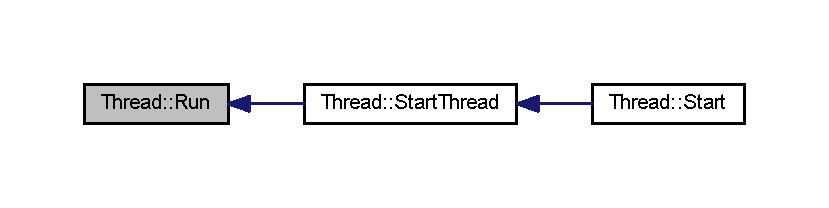
\includegraphics[width=350pt]{group___core_ae46cda1b57e998b239a8b9710b0712e2_icgraph}
\end{center}
\end{figure}


\hypertarget{group___core_ac32823199dc71dd77daba9bc9cb72c3e}{\index{Thread@{Thread}!Set\-Completed@{Set\-Completed}}
\index{Set\-Completed@{Set\-Completed}!Thread@{Thread}}
\subparagraph[{Set\-Completed}]{\setlength{\rightskip}{0pt plus 5cm}void Thread\-::\-Set\-Completed (
\begin{DoxyParamCaption}
\item[{void}]{}
\end{DoxyParamCaption}
)\hspace{0.3cm}{\ttfamily [private]}}}\label{group___core_ac32823199dc71dd77daba9bc9cb72c3e}


Here is the caller graph for this function\-:
\nopagebreak
\begin{figure}[H]
\begin{center}
\leavevmode
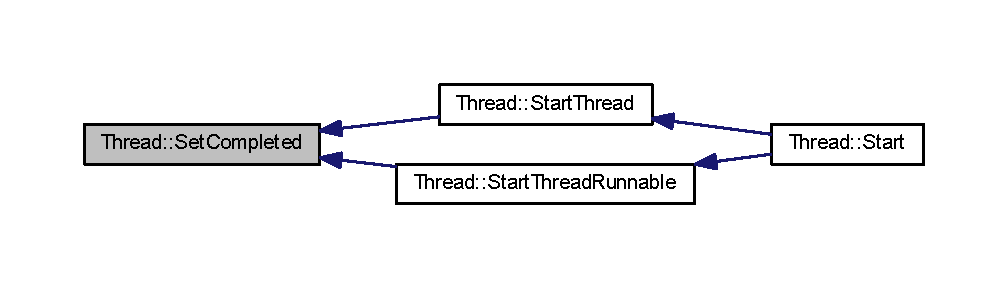
\includegraphics[width=350pt]{group___core_ac32823199dc71dd77daba9bc9cb72c3e_icgraph}
\end{center}
\end{figure}


\hypertarget{group___core_a2b42f82341afd2747ea093b6ac8b91cb}{\index{Thread@{Thread}!Start@{Start}}
\index{Start@{Start}!Thread@{Thread}}
\subparagraph[{Start}]{\setlength{\rightskip}{0pt plus 5cm}void Thread\-::\-Start (
\begin{DoxyParamCaption}
\item[{void}]{}
\end{DoxyParamCaption}
)}}\label{group___core_a2b42f82341afd2747ea093b6ac8b91cb}


Starts the thread. 



Here is the call graph for this function\-:
\nopagebreak
\begin{figure}[H]
\begin{center}
\leavevmode
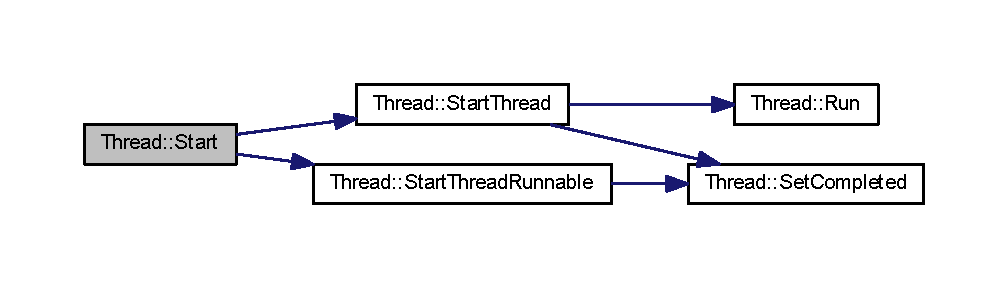
\includegraphics[width=350pt]{group___core_a2b42f82341afd2747ea093b6ac8b91cb_cgraph}
\end{center}
\end{figure}


\hypertarget{group___core_a9698abb1d7e2aed626b1963635455840}{\index{Thread@{Thread}!Start\-Thread@{Start\-Thread}}
\index{Start\-Thread@{Start\-Thread}!Thread@{Thread}}
\subparagraph[{Start\-Thread}]{\setlength{\rightskip}{0pt plus 5cm}void $\ast$ Thread\-::\-Start\-Thread (
\begin{DoxyParamCaption}
\item[{void $\ast$}]{p\-Void}
\end{DoxyParamCaption}
)\hspace{0.3cm}{\ttfamily [static]}, {\ttfamily [private]}}}\label{group___core_a9698abb1d7e2aed626b1963635455840}


\hyperlink{group___core_class_thread}{Thread} start function when no \hyperlink{group___core_class_runnable}{Runnable} is involved. 


\begin{DoxyParams}{Parameters}
{\em p\-Void} & \\
\hline
\end{DoxyParams}


Here is the call graph for this function\-:
\nopagebreak
\begin{figure}[H]
\begin{center}
\leavevmode
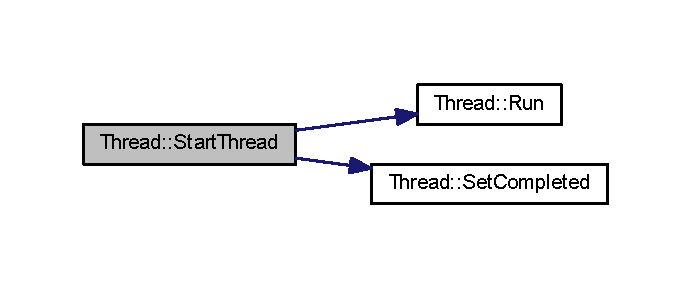
\includegraphics[width=332pt]{group___core_a9698abb1d7e2aed626b1963635455840_cgraph}
\end{center}
\end{figure}




Here is the caller graph for this function\-:
\nopagebreak
\begin{figure}[H]
\begin{center}
\leavevmode
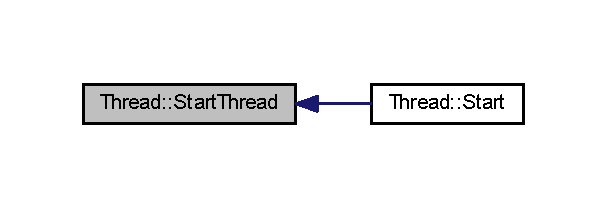
\includegraphics[width=292pt]{group___core_a9698abb1d7e2aed626b1963635455840_icgraph}
\end{center}
\end{figure}


\hypertarget{group___core_a215c9e3a0965e061e7d36aa5adfe4791}{\index{Thread@{Thread}!Start\-Thread\-Runnable@{Start\-Thread\-Runnable}}
\index{Start\-Thread\-Runnable@{Start\-Thread\-Runnable}!Thread@{Thread}}
\subparagraph[{Start\-Thread\-Runnable}]{\setlength{\rightskip}{0pt plus 5cm}void $\ast$ Thread\-::\-Start\-Thread\-Runnable (
\begin{DoxyParamCaption}
\item[{void $\ast$}]{p\-Void}
\end{DoxyParamCaption}
)\hspace{0.3cm}{\ttfamily [static]}, {\ttfamily [private]}}}\label{group___core_a215c9e3a0965e061e7d36aa5adfe4791}


\hyperlink{group___core_class_thread}{Thread} start function when a \hyperlink{group___core_class_runnable}{Runnable} is involved. 


\begin{DoxyParams}{Parameters}
{\em p\-Void} & \\
\hline
\end{DoxyParams}


Here is the call graph for this function\-:
\nopagebreak
\begin{figure}[H]
\begin{center}
\leavevmode
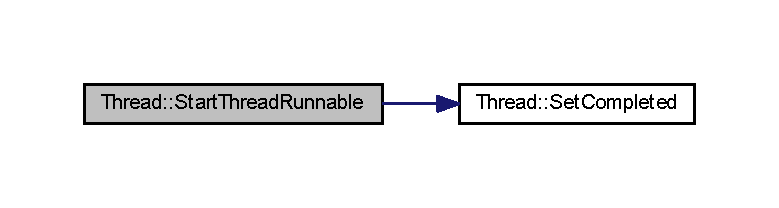
\includegraphics[width=350pt]{group___core_a215c9e3a0965e061e7d36aa5adfe4791_cgraph}
\end{center}
\end{figure}




Here is the caller graph for this function\-:
\nopagebreak
\begin{figure}[H]
\begin{center}
\leavevmode
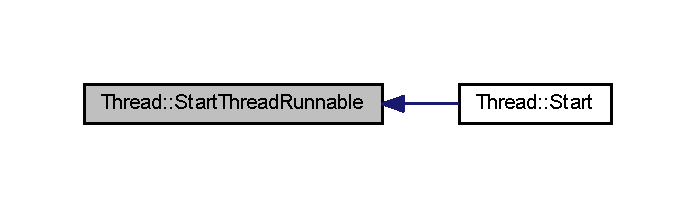
\includegraphics[width=334pt]{group___core_a215c9e3a0965e061e7d36aa5adfe4791_icgraph}
\end{center}
\end{figure}




\paragraph{Member Data Documentation}
\hypertarget{group___core_a2b6b46b7eb56cffef7d0722649956c5d}{\index{Thread@{Thread}!detached\-\_\-@{detached\-\_\-}}
\index{detached\-\_\-@{detached\-\_\-}!Thread@{Thread}}
\subparagraph[{detached\-\_\-}]{\setlength{\rightskip}{0pt plus 5cm}bool Thread\-::detached\-\_\-\hspace{0.3cm}{\ttfamily [private]}}}\label{group___core_a2b6b46b7eb56cffef7d0722649956c5d}
\hypertarget{group___core_a56c923629f0131b37a2b8c1f74a1e2b0}{\index{Thread@{Thread}!result\-\_\-@{result\-\_\-}}
\index{result\-\_\-@{result\-\_\-}!Thread@{Thread}}
\subparagraph[{result\-\_\-}]{\setlength{\rightskip}{0pt plus 5cm}void$\ast$ Thread\-::result\-\_\-\hspace{0.3cm}{\ttfamily [private]}}}\label{group___core_a56c923629f0131b37a2b8c1f74a1e2b0}
\hypertarget{group___core_a4e2c7c71f666a7c4404f8fc03a57f2d7}{\index{Thread@{Thread}!runnable\-\_\-@{runnable\-\_\-}}
\index{runnable\-\_\-@{runnable\-\_\-}!Thread@{Thread}}
\subparagraph[{runnable\-\_\-}]{\setlength{\rightskip}{0pt plus 5cm}std\-::auto\-\_\-ptr$<${\bf Runnable}$>$ Thread\-::runnable\-\_\-\hspace{0.3cm}{\ttfamily [private]}}}\label{group___core_a4e2c7c71f666a7c4404f8fc03a57f2d7}
\hypertarget{group___core_a2fbeb3f285f074698a3323bfdd7e5d2a}{\index{Thread@{Thread}!thread\-Attribute\-\_\-@{thread\-Attribute\-\_\-}}
\index{thread\-Attribute\-\_\-@{thread\-Attribute\-\_\-}!Thread@{Thread}}
\subparagraph[{thread\-Attribute\-\_\-}]{\setlength{\rightskip}{0pt plus 5cm}pthread\-\_\-attr\-\_\-t Thread\-::thread\-Attribute\-\_\-\hspace{0.3cm}{\ttfamily [private]}}}\label{group___core_a2fbeb3f285f074698a3323bfdd7e5d2a}
\hypertarget{group___core_a8a7056f4641e224b016506ec0fc1078b}{\index{Thread@{Thread}!thread\-I\-D\-\_\-@{thread\-I\-D\-\_\-}}
\index{thread\-I\-D\-\_\-@{thread\-I\-D\-\_\-}!Thread@{Thread}}
\subparagraph[{thread\-I\-D\-\_\-}]{\setlength{\rightskip}{0pt plus 5cm}pthread\-\_\-t Thread\-::thread\-I\-D\-\_\-\hspace{0.3cm}{\ttfamily [private]}}}\label{group___core_a8a7056f4641e224b016506ec0fc1078b}
\index{Visualizer@{Visualizer}}\label{class_visualizer}
\hypertarget{group___core_class_visualizer}{}
\subsubsection{class Visualizer}
Singleton window and image display manager class. \subsubsection*{Public Member Functions}
\begin{DoxyCompactItemize}
\item 
void \hyperlink{group___core_a0287f07ff905b861c4ce10a9af90d9f4}{Put\-Text} (cv\-::\-Mat \&image, const std\-::string \&text, cv\-::\-Point \&org)
\begin{DoxyCompactList}\small\item\em Renders the specified text string in the image. \end{DoxyCompactList}\item 
void \hyperlink{group___core_a51483ef2ff4337305b7ca06728eb3f1f}{Set\-Text\-Properties} (int font\-Face, double font\-Scale, cv\-::\-Scalar font\-Color, int font\-Thickness)
\begin{DoxyCompactList}\small\item\em Sets the text's properties. \end{DoxyCompactList}\item 
void \hyperlink{group___core_a910624091174d29faaa5c958215e1fd6}{Show\-Image} (const std\-::string \&name, const cv\-::\-Mat \&image, bool wait\-For\-Key=true)
\begin{DoxyCompactList}\small\item\em Creates a window and show an image within it. \end{DoxyCompactList}\end{DoxyCompactItemize}
\subsubsection*{Static Public Member Functions}
\begin{DoxyCompactItemize}
\item 
static \hyperlink{group___core_class_visualizer}{Visualizer} $\ast$ \hyperlink{group___core_a8c905f72fdc7db2ecd53ffe473340bf7}{Get\-Instance} (void)
\begin{DoxyCompactList}\small\item\em Instance getter. \end{DoxyCompactList}\end{DoxyCompactItemize}
\subsubsection*{Private Member Functions}
\begin{DoxyCompactItemize}
\item 
\hyperlink{group___core_a3611c9e093d8d855f72bcad4757ce188}{Visualizer} (void)
\begin{DoxyCompactList}\small\item\em Constructor. \end{DoxyCompactList}\item 
\hyperlink{group___core_a28c30d39ef9921a98d5b714ef1256186}{$\sim$\-Visualizer} (void)
\begin{DoxyCompactList}\small\item\em Destructor. \end{DoxyCompactList}\end{DoxyCompactItemize}
\subsubsection*{Private Attributes}
\begin{DoxyCompactItemize}
\item 
cv\-::\-Scalar \hyperlink{group___core_adc3d19a03ae171272bc5737df927027b}{font\-Color\-\_\-}
\begin{DoxyCompactList}\small\item\em Text color. \end{DoxyCompactList}\item 
int \hyperlink{group___core_a0aa6d2b6b8db04a4242fbfec555c88d1}{font\-Face\-\_\-}
\begin{DoxyCompactList}\small\item\em Font type. \end{DoxyCompactList}\item 
double \hyperlink{group___core_a9b91ed2be01274b57be07c01545ff802}{font\-Scale\-\_\-}
\begin{DoxyCompactList}\small\item\em Font scale factor that is multiplied by the font-\/specific base size. \end{DoxyCompactList}\item 
int \hyperlink{group___core_a5438944d7404d76256e5d0fb4ddecdaf}{font\-Thickness\-\_\-}
\begin{DoxyCompactList}\small\item\em Thickness of the lines used to draw a text. \end{DoxyCompactList}\end{DoxyCompactItemize}


\paragraph{Constructor \& Destructor Documentation}
\hypertarget{group___core_a3611c9e093d8d855f72bcad4757ce188}{\index{Visualizer@{Visualizer}!Visualizer@{Visualizer}}
\index{Visualizer@{Visualizer}!Visualizer@{Visualizer}}
\subparagraph[{Visualizer}]{\setlength{\rightskip}{0pt plus 5cm}Visualizer\-::\-Visualizer (
\begin{DoxyParamCaption}
\item[{void}]{}
\end{DoxyParamCaption}
)\hspace{0.3cm}{\ttfamily [private]}}}\label{group___core_a3611c9e093d8d855f72bcad4757ce188}


Constructor. 



Here is the caller graph for this function\-:
\nopagebreak
\begin{figure}[H]
\begin{center}
\leavevmode
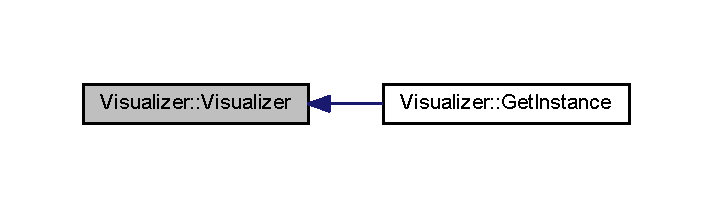
\includegraphics[width=342pt]{group___core_a3611c9e093d8d855f72bcad4757ce188_icgraph}
\end{center}
\end{figure}


\hypertarget{group___core_a28c30d39ef9921a98d5b714ef1256186}{\index{Visualizer@{Visualizer}!$\sim$\-Visualizer@{$\sim$\-Visualizer}}
\index{$\sim$\-Visualizer@{$\sim$\-Visualizer}!Visualizer@{Visualizer}}
\subparagraph[{$\sim$\-Visualizer}]{\setlength{\rightskip}{0pt plus 5cm}Visualizer\-::$\sim$\-Visualizer (
\begin{DoxyParamCaption}
\item[{void}]{}
\end{DoxyParamCaption}
)\hspace{0.3cm}{\ttfamily [private]}}}\label{group___core_a28c30d39ef9921a98d5b714ef1256186}


Destructor. 



\paragraph{Member Function Documentation}
\hypertarget{group___core_a8c905f72fdc7db2ecd53ffe473340bf7}{\index{Visualizer@{Visualizer}!Get\-Instance@{Get\-Instance}}
\index{Get\-Instance@{Get\-Instance}!Visualizer@{Visualizer}}
\subparagraph[{Get\-Instance}]{\setlength{\rightskip}{0pt plus 5cm}{\bf Visualizer} $\ast$ Visualizer\-::\-Get\-Instance (
\begin{DoxyParamCaption}
\item[{void}]{}
\end{DoxyParamCaption}
)\hspace{0.3cm}{\ttfamily [static]}}}\label{group___core_a8c905f72fdc7db2ecd53ffe473340bf7}


Instance getter. 

\begin{DoxyReturn}{Returns}
The instance. 
\end{DoxyReturn}


Here is the call graph for this function\-:
\nopagebreak
\begin{figure}[H]
\begin{center}
\leavevmode
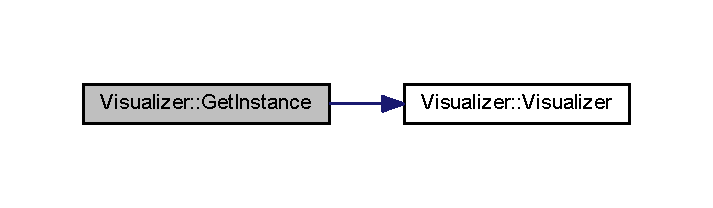
\includegraphics[width=342pt]{group___core_a8c905f72fdc7db2ecd53ffe473340bf7_cgraph}
\end{center}
\end{figure}


\hypertarget{group___core_a0287f07ff905b861c4ce10a9af90d9f4}{\index{Visualizer@{Visualizer}!Put\-Text@{Put\-Text}}
\index{Put\-Text@{Put\-Text}!Visualizer@{Visualizer}}
\subparagraph[{Put\-Text}]{\setlength{\rightskip}{0pt plus 5cm}void Visualizer\-::\-Put\-Text (
\begin{DoxyParamCaption}
\item[{cv\-::\-Mat \&}]{image, }
\item[{const std\-::string \&}]{text, }
\item[{cv\-::\-Point \&}]{org}
\end{DoxyParamCaption}
)}}\label{group___core_a0287f07ff905b861c4ce10a9af90d9f4}


Renders the specified text string in the image. 


\begin{DoxyParams}{Parameters}
{\em image} & Image. \\
\hline
{\em text} & Text string to be drawn. \\
\hline
{\em org} & Bottom-\/left corner of the text string in the image. \\
\hline
\end{DoxyParams}
\hypertarget{group___core_a51483ef2ff4337305b7ca06728eb3f1f}{\index{Visualizer@{Visualizer}!Set\-Text\-Properties@{Set\-Text\-Properties}}
\index{Set\-Text\-Properties@{Set\-Text\-Properties}!Visualizer@{Visualizer}}
\subparagraph[{Set\-Text\-Properties}]{\setlength{\rightskip}{0pt plus 5cm}void Visualizer\-::\-Set\-Text\-Properties (
\begin{DoxyParamCaption}
\item[{int}]{font\-Face, }
\item[{double}]{font\-Scale, }
\item[{cv\-::\-Scalar}]{font\-Color, }
\item[{int}]{font\-Thickness}
\end{DoxyParamCaption}
)}}\label{group___core_a51483ef2ff4337305b7ca06728eb3f1f}


Sets the text's properties. 


\begin{DoxyParams}{Parameters}
{\em font\-Face} & Font type. \\
\hline
{\em font\-Scale} & Font scale factor that is multiplied by the font-\/specific base size. \\
\hline
{\em font\-Color} & Text color. \\
\hline
{\em font\-Thickness} & Thickness of the lines used to draw a text. \\
\hline
\end{DoxyParams}
\hypertarget{group___core_a910624091174d29faaa5c958215e1fd6}{\index{Visualizer@{Visualizer}!Show\-Image@{Show\-Image}}
\index{Show\-Image@{Show\-Image}!Visualizer@{Visualizer}}
\subparagraph[{Show\-Image}]{\setlength{\rightskip}{0pt plus 5cm}void Visualizer\-::\-Show\-Image (
\begin{DoxyParamCaption}
\item[{const std\-::string \&}]{name, }
\item[{const cv\-::\-Mat \&}]{image, }
\item[{bool}]{wait\-For\-Key = {\ttfamily true}}
\end{DoxyParamCaption}
)}}\label{group___core_a910624091174d29faaa5c958215e1fd6}


Creates a window and show an image within it. 


\begin{DoxyParams}{Parameters}
{\em name} & Name of the window. \\
\hline
{\em image} & Image to be shown. \\
\hline
{\em wait\-For\-Key} & Waits for a pressed key. \\
\hline
\end{DoxyParams}


\paragraph{Member Data Documentation}
\hypertarget{group___core_adc3d19a03ae171272bc5737df927027b}{\index{Visualizer@{Visualizer}!font\-Color\-\_\-@{font\-Color\-\_\-}}
\index{font\-Color\-\_\-@{font\-Color\-\_\-}!Visualizer@{Visualizer}}
\subparagraph[{font\-Color\-\_\-}]{\setlength{\rightskip}{0pt plus 5cm}cv\-::\-Scalar Visualizer\-::font\-Color\-\_\-\hspace{0.3cm}{\ttfamily [private]}}}\label{group___core_adc3d19a03ae171272bc5737df927027b}


Text color. 

\hypertarget{group___core_a0aa6d2b6b8db04a4242fbfec555c88d1}{\index{Visualizer@{Visualizer}!font\-Face\-\_\-@{font\-Face\-\_\-}}
\index{font\-Face\-\_\-@{font\-Face\-\_\-}!Visualizer@{Visualizer}}
\subparagraph[{font\-Face\-\_\-}]{\setlength{\rightskip}{0pt plus 5cm}int Visualizer\-::font\-Face\-\_\-\hspace{0.3cm}{\ttfamily [private]}}}\label{group___core_a0aa6d2b6b8db04a4242fbfec555c88d1}


Font type. 

\hypertarget{group___core_a9b91ed2be01274b57be07c01545ff802}{\index{Visualizer@{Visualizer}!font\-Scale\-\_\-@{font\-Scale\-\_\-}}
\index{font\-Scale\-\_\-@{font\-Scale\-\_\-}!Visualizer@{Visualizer}}
\subparagraph[{font\-Scale\-\_\-}]{\setlength{\rightskip}{0pt plus 5cm}double Visualizer\-::font\-Scale\-\_\-\hspace{0.3cm}{\ttfamily [private]}}}\label{group___core_a9b91ed2be01274b57be07c01545ff802}


Font scale factor that is multiplied by the font-\/specific base size. 

\hypertarget{group___core_a5438944d7404d76256e5d0fb4ddecdaf}{\index{Visualizer@{Visualizer}!font\-Thickness\-\_\-@{font\-Thickness\-\_\-}}
\index{font\-Thickness\-\_\-@{font\-Thickness\-\_\-}!Visualizer@{Visualizer}}
\subparagraph[{font\-Thickness\-\_\-}]{\setlength{\rightskip}{0pt plus 5cm}int Visualizer\-::font\-Thickness\-\_\-\hspace{0.3cm}{\ttfamily [private]}}}\label{group___core_a5438944d7404d76256e5d0fb4ddecdaf}


Thickness of the lines used to draw a text. 


\hypertarget{group___feature_extractor}{\section{Feature\-Extractor module.}
\label{group___feature_extractor}\index{Feature\-Extractor module.@{Feature\-Extractor module.}}
}
\subsection*{Classes}
\begin{DoxyCompactItemize}
\item 
class \hyperlink{group___feature_extractor_class_fast_feature}{Fast\-Feature}
\begin{DoxyCompactList}\small\item\em Class for extracting F\-A\-S\-T features.  \hyperlink{group___feature_extractor_class_fast_feature}{More...}\end{DoxyCompactList}\item 
class \hyperlink{group___feature_extractor_class_global_feature}{Global\-Feature}
\begin{DoxyCompactList}\small\item\em Abstract class for global feature extraction.  \hyperlink{group___feature_extractor_class_global_feature}{More...}\end{DoxyCompactList}\item 
class \hyperlink{group___feature_extractor_class_lbp_feature}{Lbp\-Feature}
\begin{DoxyCompactList}\small\item\em Class for extracting L\-B\-P features.  \hyperlink{group___feature_extractor_class_lbp_feature}{More...}\end{DoxyCompactList}\item 
class \hyperlink{group___feature_extractor_class_local_feature}{Local\-Feature}
\begin{DoxyCompactList}\small\item\em Abstract class for local feature extraction.  \hyperlink{group___feature_extractor_class_local_feature}{More...}\end{DoxyCompactList}\item 
class \hyperlink{group___feature_extractor_class_mser_feature}{Mser\-Feature}
\begin{DoxyCompactList}\small\item\em Class for extracting M\-S\-E\-R features.  \hyperlink{group___feature_extractor_class_mser_feature}{More...}\end{DoxyCompactList}\item 
class \hyperlink{group___feature_extractor_class_orb_feature}{Orb\-Feature}
\begin{DoxyCompactList}\small\item\em Class for extracting O\-R\-B features.  \hyperlink{group___feature_extractor_class_orb_feature}{More...}\end{DoxyCompactList}\item 
class \hyperlink{group___feature_extractor_class_sift_feature}{Sift\-Feature}
\begin{DoxyCompactList}\small\item\em Class for extracting S\-I\-F\-T features.  \hyperlink{group___feature_extractor_class_sift_feature}{More...}\end{DoxyCompactList}\item 
class \hyperlink{group___feature_extractor_class_star_feature}{Star\-Feature}
\begin{DoxyCompactList}\small\item\em Class for extracting S\-T\-A\-R features.  \hyperlink{group___feature_extractor_class_star_feature}{More...}\end{DoxyCompactList}\item 
class \hyperlink{group___feature_extractor_class_surf_feature}{Surf\-Feature}
\begin{DoxyCompactList}\small\item\em Class for extracting S\-U\-R\-F features.  \hyperlink{group___feature_extractor_class_surf_feature}{More...}\end{DoxyCompactList}\end{DoxyCompactItemize}


\subsection{Detailed Description}


\subsection{Class Documentation}
\index{Fast\-Feature@{Fast\-Feature}}\label{class_fast_feature}
\hypertarget{group___feature_extractor_class_fast_feature}{}
\subsubsection{class Fast\-Feature}
Class for extracting F\-A\-S\-T features. 

\begin{DoxyVerb}Detects corners using the FAST algorithm.
\end{DoxyVerb}


See paper\-: E. Rosten. Machine Learning for High-\/speed Corner Detection, 2006. 

Inheritance diagram for Fast\-Feature\-:
\nopagebreak
\begin{figure}[H]
\begin{center}
\leavevmode
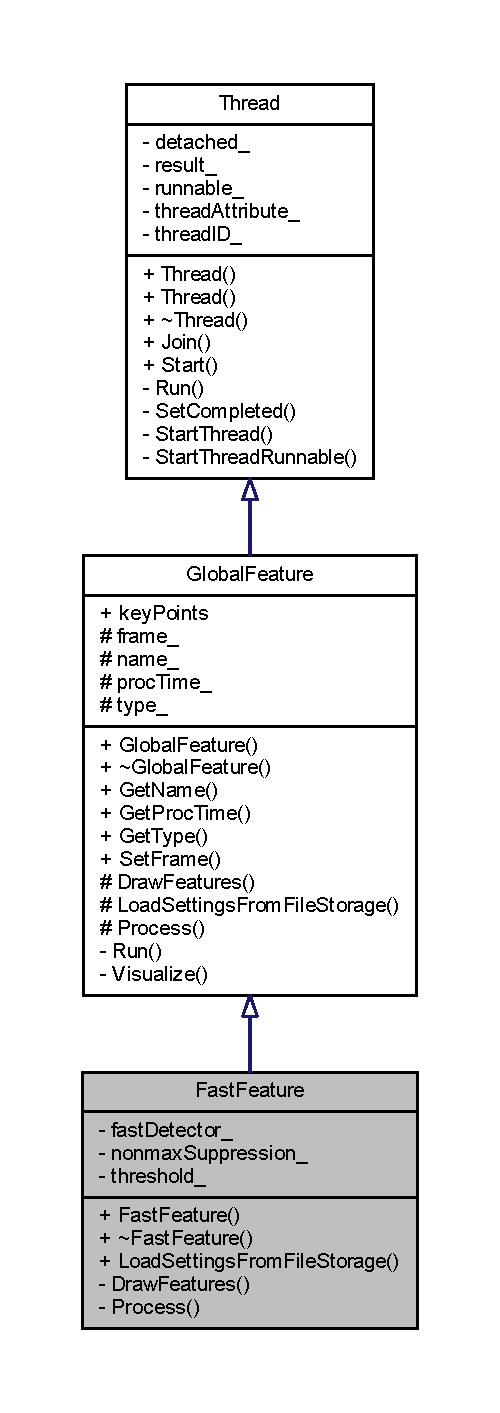
\includegraphics[height=550pt]{class_fast_feature__inherit__graph}
\end{center}
\end{figure}


Collaboration diagram for Fast\-Feature\-:
\nopagebreak
\begin{figure}[H]
\begin{center}
\leavevmode
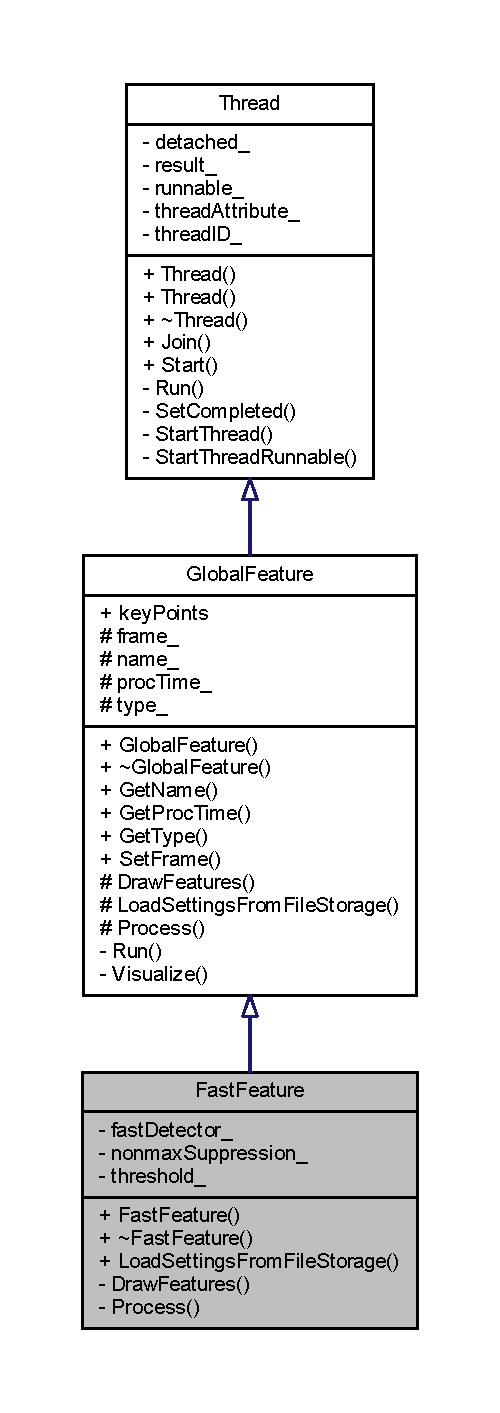
\includegraphics[height=550pt]{class_fast_feature__coll__graph}
\end{center}
\end{figure}
\subsubsection*{Public Member Functions}
\begin{DoxyCompactItemize}
\item 
\hyperlink{group___feature_extractor_a5e30312c922a9006209e601475c3cd11}{Fast\-Feature} (const std\-::string \&name, const std\-::string \&type)
\begin{DoxyCompactList}\small\item\em Constructor. \end{DoxyCompactList}\item 
\hyperlink{group___feature_extractor_a32a012aa9fef7fdf88d062421d76ab35}{$\sim$\-Fast\-Feature} (void)
\begin{DoxyCompactList}\small\item\em Destructor. \end{DoxyCompactList}\item 
const std\-::string \& \hyperlink{group___feature_extractor_a5f69ca2455d5eec4493dbf115d00d5c9}{Get\-Name} (void)
\begin{DoxyCompactList}\small\item\em Name getter. \end{DoxyCompactList}\item 
double \hyperlink{group___feature_extractor_ad07a3104192b50d911eee634a0be009d}{Get\-Proc\-Time} (void)
\begin{DoxyCompactList}\small\item\em Process time getter. \end{DoxyCompactList}\item 
const std\-::string \& \hyperlink{group___feature_extractor_a6724c19006d495bd6a9c8c6029236ebc}{Get\-Type} (void)
\begin{DoxyCompactList}\small\item\em Type getter. \end{DoxyCompactList}\item 
void $\ast$ \hyperlink{group___core_a8f33f7750321d5df9188033e7e3e300d}{Join} (void)
\item 
void \hyperlink{group___feature_extractor_a341ffc5bd43e0ee09fda3fe6f825acba}{Load\-Settings\-From\-File\-Storage} (void)
\begin{DoxyCompactList}\small\item\em Implemented virtual method for loading algorithm specific settings from the given storage. \end{DoxyCompactList}\item 
void \hyperlink{group___feature_extractor_a3c58d995fb2440b28db3b21b54b94815}{Set\-Frame} (const cv\-::\-Mat \&frame)
\begin{DoxyCompactList}\small\item\em Connects a frame to the feature extractor. \end{DoxyCompactList}\item 
void \hyperlink{group___core_a2b42f82341afd2747ea093b6ac8b91cb}{Start} (void)
\begin{DoxyCompactList}\small\item\em Starts the thread. \end{DoxyCompactList}\end{DoxyCompactItemize}
\subsubsection*{Public Attributes}
\begin{DoxyCompactItemize}
\item 
std\-::vector$<$ cv\-::\-Key\-Point $>$ \hyperlink{group___feature_extractor_a72cc606c0090a64718a7e92bca7520b9}{key\-Points}
\begin{DoxyCompactList}\small\item\em Stores keypoints, i.\-e. a point feature found by one of many available keypoint detectors. \end{DoxyCompactList}\end{DoxyCompactItemize}
\subsubsection*{Protected Attributes}
\begin{DoxyCompactItemize}
\item 
cv\-::\-Mat \hyperlink{group___feature_extractor_aae4295da2c3999edcb99b46d70ee7166}{frame\-\_\-}
\begin{DoxyCompactList}\small\item\em The current frame. \end{DoxyCompactList}\item 
std\-::string \hyperlink{group___feature_extractor_abee52be830de272bd27685083bf28aae}{name\-\_\-}
\begin{DoxyCompactList}\small\item\em Name of the current feature extraction procedure. \end{DoxyCompactList}\item 
double \hyperlink{group___feature_extractor_aa3306975b929f5503dac51829f9e04a0}{proc\-Time\-\_\-}
\begin{DoxyCompactList}\small\item\em Processing time of the current feature extraction method. \end{DoxyCompactList}\item 
std\-::string \hyperlink{group___feature_extractor_ad467857c4bc3d0fe65ba29e3b8f7c796}{type\-\_\-}
\begin{DoxyCompactList}\small\item\em Type of the current feature extraction procedure. \end{DoxyCompactList}\end{DoxyCompactItemize}
\subsubsection*{Private Member Functions}
\begin{DoxyCompactItemize}
\item 
void \hyperlink{group___feature_extractor_a765f433c231d5f0d088beeaa77aa0e7a}{Draw\-Features} (void)
\begin{DoxyCompactList}\small\item\em Implemented virtual method for displaying the output. \end{DoxyCompactList}\item 
void \hyperlink{group___feature_extractor_a4bbf87c97bd86bf44d4c021b053a7e66}{Process} (void)
\begin{DoxyCompactList}\small\item\em Implemented virtual method for the algorithm. \end{DoxyCompactList}\end{DoxyCompactItemize}
\subsubsection*{Private Attributes}
\begin{DoxyCompactItemize}
\item 
cv\-::\-Fast\-Feature\-Detector $\ast$ \hyperlink{group___feature_extractor_a4978fabcb2c02a6828672ecf09b1fbec}{fast\-Detector\-\_\-}
\begin{DoxyCompactList}\small\item\em Wrapped Open\-C\-V F\-A\-S\-T object. \end{DoxyCompactList}\item 
bool \hyperlink{group___feature_extractor_afc991a85e5ee2d8f1a52657eee8d380d}{nonmax\-Suppression\-\_\-}
\begin{DoxyCompactList}\small\item\em If it is true, non-\/maximum suppression is applied to detected corners (keypoints). \end{DoxyCompactList}\item 
int \hyperlink{group___feature_extractor_afc261d12e34223dc377b1ea8f8d3a773}{threshold\-\_\-}
\begin{DoxyCompactList}\small\item\em Threshold on difference between intensity of the central pixel and pixels on a circle around this pixel. \end{DoxyCompactList}\end{DoxyCompactItemize}


\paragraph{Constructor \& Destructor Documentation}
\hypertarget{group___feature_extractor_a5e30312c922a9006209e601475c3cd11}{\index{Fast\-Feature@{Fast\-Feature}!Fast\-Feature@{Fast\-Feature}}
\index{Fast\-Feature@{Fast\-Feature}!FastFeature@{Fast\-Feature}}
\subparagraph[{Fast\-Feature}]{\setlength{\rightskip}{0pt plus 5cm}Fast\-Feature\-::\-Fast\-Feature (
\begin{DoxyParamCaption}
\item[{const std\-::string \&}]{name, }
\item[{const std\-::string \&}]{type}
\end{DoxyParamCaption}
)}}\label{group___feature_extractor_a5e30312c922a9006209e601475c3cd11}


Constructor. 

\begin{DoxyVerb}    \param name Name of the current feature extraction procedure.
\end{DoxyVerb}
 
\begin{DoxyParams}{Parameters}
{\em type} & Type of the current feature extraction procedure (global or local). \\
\hline
\end{DoxyParams}


References fast\-Detector\-\_\-, Load\-Settings\-From\-File\-Storage(), nonmax\-Suppression\-\_\-, and threshold\-\_\-.



Here is the call graph for this function\-:
\nopagebreak
\begin{figure}[H]
\begin{center}
\leavevmode
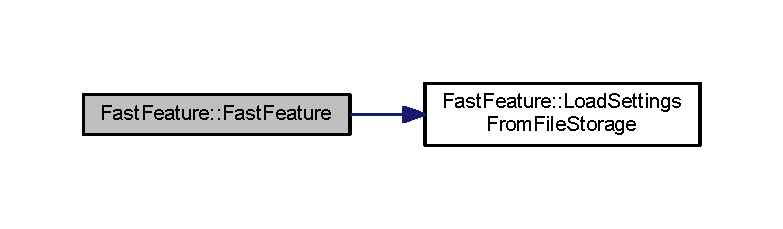
\includegraphics[width=350pt]{group___feature_extractor_a5e30312c922a9006209e601475c3cd11_cgraph}
\end{center}
\end{figure}


\hypertarget{group___feature_extractor_a32a012aa9fef7fdf88d062421d76ab35}{\index{Fast\-Feature@{Fast\-Feature}!$\sim$\-Fast\-Feature@{$\sim$\-Fast\-Feature}}
\index{$\sim$\-Fast\-Feature@{$\sim$\-Fast\-Feature}!FastFeature@{Fast\-Feature}}
\subparagraph[{$\sim$\-Fast\-Feature}]{\setlength{\rightskip}{0pt plus 5cm}Fast\-Feature\-::$\sim$\-Fast\-Feature (
\begin{DoxyParamCaption}
\item[{void}]{}
\end{DoxyParamCaption}
)}}\label{group___feature_extractor_a32a012aa9fef7fdf88d062421d76ab35}


Destructor. 



References fast\-Detector\-\_\-.



\paragraph{Member Function Documentation}
\hypertarget{group___feature_extractor_a765f433c231d5f0d088beeaa77aa0e7a}{\index{Fast\-Feature@{Fast\-Feature}!Draw\-Features@{Draw\-Features}}
\index{Draw\-Features@{Draw\-Features}!FastFeature@{Fast\-Feature}}
\subparagraph[{Draw\-Features}]{\setlength{\rightskip}{0pt plus 5cm}void Fast\-Feature\-::\-Draw\-Features (
\begin{DoxyParamCaption}
\item[{void}]{}
\end{DoxyParamCaption}
)\hspace{0.3cm}{\ttfamily [private]}, {\ttfamily [virtual]}}}\label{group___feature_extractor_a765f433c231d5f0d088beeaa77aa0e7a}


Implemented virtual method for displaying the output. 

\begin{DoxySeeAlso}{See Also}
\hyperlink{group___feature_extractor_acea1ee12c177894819ea7ae0f6294e5c}{Global\-Feature\-::\-Draw\-Features()} 
\end{DoxySeeAlso}


Reimplemented from \hyperlink{group___feature_extractor_acea1ee12c177894819ea7ae0f6294e5c}{Global\-Feature}.



References Global\-Feature\-::frame\-\_\-, and Global\-Feature\-::key\-Points.

\hypertarget{group___feature_extractor_a5f69ca2455d5eec4493dbf115d00d5c9}{\index{Fast\-Feature@{Fast\-Feature}!Get\-Name@{Get\-Name}}
\index{Get\-Name@{Get\-Name}!FastFeature@{Fast\-Feature}}
\subparagraph[{Get\-Name}]{\setlength{\rightskip}{0pt plus 5cm}const string \& Global\-Feature\-::\-Get\-Name (
\begin{DoxyParamCaption}
\item[{void}]{}
\end{DoxyParamCaption}
)\hspace{0.3cm}{\ttfamily [inherited]}}}\label{group___feature_extractor_a5f69ca2455d5eec4493dbf115d00d5c9}


Name getter. 

\begin{DoxyReturn}{Returns}
Name of the current feature extraction procedure. 
\end{DoxyReturn}


References Global\-Feature\-::name\-\_\-.

\hypertarget{group___feature_extractor_ad07a3104192b50d911eee634a0be009d}{\index{Fast\-Feature@{Fast\-Feature}!Get\-Proc\-Time@{Get\-Proc\-Time}}
\index{Get\-Proc\-Time@{Get\-Proc\-Time}!FastFeature@{Fast\-Feature}}
\subparagraph[{Get\-Proc\-Time}]{\setlength{\rightskip}{0pt plus 5cm}double Global\-Feature\-::\-Get\-Proc\-Time (
\begin{DoxyParamCaption}
\item[{void}]{}
\end{DoxyParamCaption}
)\hspace{0.3cm}{\ttfamily [inherited]}}}\label{group___feature_extractor_ad07a3104192b50d911eee634a0be009d}


Process time getter. 

\begin{DoxyReturn}{Returns}
Processing time of the current feature extraction method. 
\end{DoxyReturn}


References Global\-Feature\-::proc\-Time\-\_\-.

\hypertarget{group___feature_extractor_a6724c19006d495bd6a9c8c6029236ebc}{\index{Fast\-Feature@{Fast\-Feature}!Get\-Type@{Get\-Type}}
\index{Get\-Type@{Get\-Type}!FastFeature@{Fast\-Feature}}
\subparagraph[{Get\-Type}]{\setlength{\rightskip}{0pt plus 5cm}const string \& Global\-Feature\-::\-Get\-Type (
\begin{DoxyParamCaption}
\item[{void}]{}
\end{DoxyParamCaption}
)\hspace{0.3cm}{\ttfamily [inherited]}}}\label{group___feature_extractor_a6724c19006d495bd6a9c8c6029236ebc}


Type getter. 

\begin{DoxyReturn}{Returns}
Type of the current feature extraction procedure. 
\end{DoxyReturn}


References Global\-Feature\-::type\-\_\-.

\hypertarget{group___core_a8f33f7750321d5df9188033e7e3e300d}{\index{Fast\-Feature@{Fast\-Feature}!Join@{Join}}
\index{Join@{Join}!FastFeature@{Fast\-Feature}}
\subparagraph[{Join}]{\setlength{\rightskip}{0pt plus 5cm}void $\ast$ Thread\-::\-Join (
\begin{DoxyParamCaption}
\item[{void}]{}
\end{DoxyParamCaption}
)\hspace{0.3cm}{\ttfamily [inherited]}}}\label{group___core_a8f33f7750321d5df9188033e7e3e300d}


References Exception\-Error, Thread\-::result\-\_\-, and Thread\-::thread\-I\-D\-\_\-.

\hypertarget{group___feature_extractor_a341ffc5bd43e0ee09fda3fe6f825acba}{\index{Fast\-Feature@{Fast\-Feature}!Load\-Settings\-From\-File\-Storage@{Load\-Settings\-From\-File\-Storage}}
\index{Load\-Settings\-From\-File\-Storage@{Load\-Settings\-From\-File\-Storage}!FastFeature@{Fast\-Feature}}
\subparagraph[{Load\-Settings\-From\-File\-Storage}]{\setlength{\rightskip}{0pt plus 5cm}void Fast\-Feature\-::\-Load\-Settings\-From\-File\-Storage (
\begin{DoxyParamCaption}
\item[{void}]{}
\end{DoxyParamCaption}
)\hspace{0.3cm}{\ttfamily [virtual]}}}\label{group___feature_extractor_a341ffc5bd43e0ee09fda3fe6f825acba}


Implemented virtual method for loading algorithm specific settings from the given storage. 

\begin{DoxySeeAlso}{See Also}
\hyperlink{group___feature_extractor_aa48133762d9f52a5c2ae5042f6ebbe71}{Global\-Feature\-::\-Load\-Settings\-From\-File\-Storage()} 
\end{DoxySeeAlso}


Reimplemented from \hyperlink{group___feature_extractor_aa48133762d9f52a5c2ae5042f6ebbe71}{Global\-Feature}.



References Exception\-Error, Local\-Settings\-Ptr, Global\-Feature\-::name\-\_\-, nonmax\-Suppression\-\_\-, and threshold\-\_\-.



Referenced by Fast\-Feature().



Here is the caller graph for this function\-:
\nopagebreak
\begin{figure}[H]
\begin{center}
\leavevmode
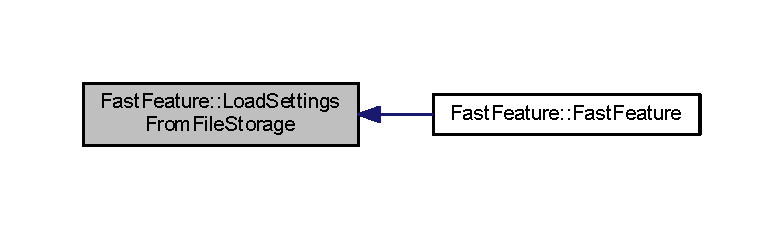
\includegraphics[width=350pt]{group___feature_extractor_a341ffc5bd43e0ee09fda3fe6f825acba_icgraph}
\end{center}
\end{figure}


\hypertarget{group___feature_extractor_a4bbf87c97bd86bf44d4c021b053a7e66}{\index{Fast\-Feature@{Fast\-Feature}!Process@{Process}}
\index{Process@{Process}!FastFeature@{Fast\-Feature}}
\subparagraph[{Process}]{\setlength{\rightskip}{0pt plus 5cm}void Fast\-Feature\-::\-Process (
\begin{DoxyParamCaption}
\item[{void}]{}
\end{DoxyParamCaption}
)\hspace{0.3cm}{\ttfamily [private]}, {\ttfamily [virtual]}}}\label{group___feature_extractor_a4bbf87c97bd86bf44d4c021b053a7e66}


Implemented virtual method for the algorithm. 

\begin{DoxySeeAlso}{See Also}
\hyperlink{group___feature_extractor_a9fdfc934c5a9da6962ec39c1b0cf32dc}{Global\-Feature\-::\-Process()} 
\end{DoxySeeAlso}


Reimplemented from \hyperlink{group___feature_extractor_a9fdfc934c5a9da6962ec39c1b0cf32dc}{Global\-Feature}.



References fast\-Detector\-\_\-, Global\-Feature\-::frame\-\_\-, and Global\-Feature\-::key\-Points.

\hypertarget{group___feature_extractor_a3c58d995fb2440b28db3b21b54b94815}{\index{Fast\-Feature@{Fast\-Feature}!Set\-Frame@{Set\-Frame}}
\index{Set\-Frame@{Set\-Frame}!FastFeature@{Fast\-Feature}}
\subparagraph[{Set\-Frame}]{\setlength{\rightskip}{0pt plus 5cm}void Global\-Feature\-::\-Set\-Frame (
\begin{DoxyParamCaption}
\item[{const cv\-::\-Mat \&}]{frame}
\end{DoxyParamCaption}
)\hspace{0.3cm}{\ttfamily [inherited]}}}\label{group___feature_extractor_a3c58d995fb2440b28db3b21b54b94815}


Connects a frame to the feature extractor. 


\begin{DoxyParams}{Parameters}
{\em frame} & Output parameter for the current frame. \\
\hline
\end{DoxyParams}


References Global\-Feature\-::frame\-\_\-.

\hypertarget{group___core_a2b42f82341afd2747ea093b6ac8b91cb}{\index{Fast\-Feature@{Fast\-Feature}!Start@{Start}}
\index{Start@{Start}!FastFeature@{Fast\-Feature}}
\subparagraph[{Start}]{\setlength{\rightskip}{0pt plus 5cm}void Thread\-::\-Start (
\begin{DoxyParamCaption}
\item[{void}]{}
\end{DoxyParamCaption}
)\hspace{0.3cm}{\ttfamily [inherited]}}}\label{group___core_a2b42f82341afd2747ea093b6ac8b91cb}


Starts the thread. 



References Thread\-::detached\-\_\-, Exception\-Error, Thread\-::runnable\-\_\-, Thread\-::\-Start\-Thread(), Thread\-::\-Start\-Thread\-Runnable(), Thread\-::thread\-Attribute\-\_\-, and Thread\-::thread\-I\-D\-\_\-.



Here is the call graph for this function\-:
\nopagebreak
\begin{figure}[H]
\begin{center}
\leavevmode
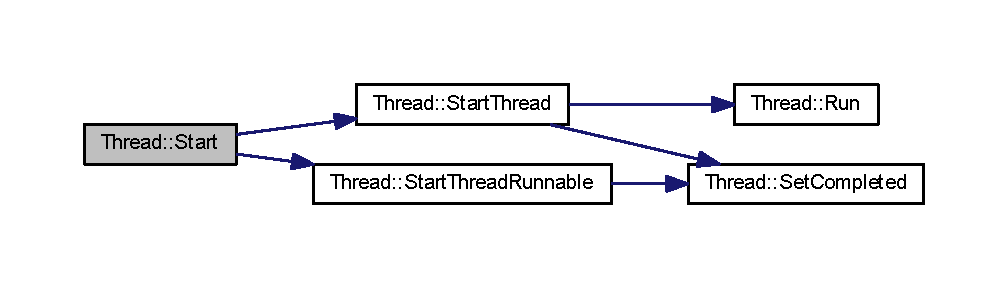
\includegraphics[width=350pt]{group___core_a2b42f82341afd2747ea093b6ac8b91cb_cgraph}
\end{center}
\end{figure}




\paragraph{Member Data Documentation}
\hypertarget{group___feature_extractor_a4978fabcb2c02a6828672ecf09b1fbec}{\index{Fast\-Feature@{Fast\-Feature}!fast\-Detector\-\_\-@{fast\-Detector\-\_\-}}
\index{fast\-Detector\-\_\-@{fast\-Detector\-\_\-}!FastFeature@{Fast\-Feature}}
\subparagraph[{fast\-Detector\-\_\-}]{\setlength{\rightskip}{0pt plus 5cm}cv\-::\-Fast\-Feature\-Detector$\ast$ Fast\-Feature\-::fast\-Detector\-\_\-\hspace{0.3cm}{\ttfamily [private]}}}\label{group___feature_extractor_a4978fabcb2c02a6828672ecf09b1fbec}


Wrapped Open\-C\-V F\-A\-S\-T object. 



Referenced by Fast\-Feature(), Process(), and $\sim$\-Fast\-Feature().

\hypertarget{group___feature_extractor_aae4295da2c3999edcb99b46d70ee7166}{\index{Fast\-Feature@{Fast\-Feature}!frame\-\_\-@{frame\-\_\-}}
\index{frame\-\_\-@{frame\-\_\-}!FastFeature@{Fast\-Feature}}
\subparagraph[{frame\-\_\-}]{\setlength{\rightskip}{0pt plus 5cm}cv\-::\-Mat Global\-Feature\-::frame\-\_\-\hspace{0.3cm}{\ttfamily [protected]}, {\ttfamily [inherited]}}}\label{group___feature_extractor_aae4295da2c3999edcb99b46d70ee7166}


The current frame. 



Referenced by Mser\-Feature\-::\-Draw\-Features(), Star\-Feature\-::\-Draw\-Features(), Orb\-Feature\-::\-Draw\-Features(), Sift\-Feature\-::\-Draw\-Features(), Draw\-Features(), Surf\-Feature\-::\-Draw\-Features(), Star\-Feature\-::\-Process(), Mser\-Feature\-::\-Process(), Process(), Orb\-Feature\-::\-Process(), Surf\-Feature\-::\-Process(), Sift\-Feature\-::\-Process(), Global\-Feature\-::\-Run(), Global\-Feature\-::\-Set\-Frame(), and Global\-Feature\-::\-Visualize().

\hypertarget{group___feature_extractor_a72cc606c0090a64718a7e92bca7520b9}{\index{Fast\-Feature@{Fast\-Feature}!key\-Points@{key\-Points}}
\index{key\-Points@{key\-Points}!FastFeature@{Fast\-Feature}}
\subparagraph[{key\-Points}]{\setlength{\rightskip}{0pt plus 5cm}std\-::vector$<$cv\-::\-Key\-Point$>$ Global\-Feature\-::key\-Points\hspace{0.3cm}{\ttfamily [inherited]}}}\label{group___feature_extractor_a72cc606c0090a64718a7e92bca7520b9}


Stores keypoints, i.\-e. a point feature found by one of many available keypoint detectors. 



Referenced by Mser\-Feature\-::\-Draw\-Features(), Star\-Feature\-::\-Draw\-Features(), Sift\-Feature\-::\-Draw\-Features(), Draw\-Features(), Orb\-Feature\-::\-Draw\-Features(), Surf\-Feature\-::\-Draw\-Features(), Mser\-Feature\-::\-Process(), Star\-Feature\-::\-Process(), Orb\-Feature\-::\-Process(), Sift\-Feature\-::\-Process(), Surf\-Feature\-::\-Process(), Process(), and Global\-Feature\-::\-Visualize().

\hypertarget{group___feature_extractor_abee52be830de272bd27685083bf28aae}{\index{Fast\-Feature@{Fast\-Feature}!name\-\_\-@{name\-\_\-}}
\index{name\-\_\-@{name\-\_\-}!FastFeature@{Fast\-Feature}}
\subparagraph[{name\-\_\-}]{\setlength{\rightskip}{0pt plus 5cm}std\-::string Global\-Feature\-::name\-\_\-\hspace{0.3cm}{\ttfamily [protected]}, {\ttfamily [inherited]}}}\label{group___feature_extractor_abee52be830de272bd27685083bf28aae}


Name of the current feature extraction procedure. 



Referenced by Global\-Feature\-::\-Get\-Name(), Mser\-Feature\-::\-Load\-Settings\-From\-File\-Storage(), Star\-Feature\-::\-Load\-Settings\-From\-File\-Storage(), Sift\-Feature\-::\-Load\-Settings\-From\-File\-Storage(), Orb\-Feature\-::\-Load\-Settings\-From\-File\-Storage(), Surf\-Feature\-::\-Load\-Settings\-From\-File\-Storage(), Load\-Settings\-From\-File\-Storage(), and Global\-Feature\-::\-Visualize().

\hypertarget{group___feature_extractor_afc991a85e5ee2d8f1a52657eee8d380d}{\index{Fast\-Feature@{Fast\-Feature}!nonmax\-Suppression\-\_\-@{nonmax\-Suppression\-\_\-}}
\index{nonmax\-Suppression\-\_\-@{nonmax\-Suppression\-\_\-}!FastFeature@{Fast\-Feature}}
\subparagraph[{nonmax\-Suppression\-\_\-}]{\setlength{\rightskip}{0pt plus 5cm}bool Fast\-Feature\-::nonmax\-Suppression\-\_\-\hspace{0.3cm}{\ttfamily [private]}}}\label{group___feature_extractor_afc991a85e5ee2d8f1a52657eee8d380d}


If it is true, non-\/maximum suppression is applied to detected corners (keypoints). 



Referenced by Fast\-Feature(), and Load\-Settings\-From\-File\-Storage().

\hypertarget{group___feature_extractor_aa3306975b929f5503dac51829f9e04a0}{\index{Fast\-Feature@{Fast\-Feature}!proc\-Time\-\_\-@{proc\-Time\-\_\-}}
\index{proc\-Time\-\_\-@{proc\-Time\-\_\-}!FastFeature@{Fast\-Feature}}
\subparagraph[{proc\-Time\-\_\-}]{\setlength{\rightskip}{0pt plus 5cm}double Global\-Feature\-::proc\-Time\-\_\-\hspace{0.3cm}{\ttfamily [protected]}, {\ttfamily [inherited]}}}\label{group___feature_extractor_aa3306975b929f5503dac51829f9e04a0}


Processing time of the current feature extraction method. 



Referenced by Global\-Feature\-::\-Get\-Proc\-Time(), Global\-Feature\-::\-Run(), and Global\-Feature\-::\-Visualize().

\hypertarget{group___feature_extractor_afc261d12e34223dc377b1ea8f8d3a773}{\index{Fast\-Feature@{Fast\-Feature}!threshold\-\_\-@{threshold\-\_\-}}
\index{threshold\-\_\-@{threshold\-\_\-}!FastFeature@{Fast\-Feature}}
\subparagraph[{threshold\-\_\-}]{\setlength{\rightskip}{0pt plus 5cm}int Fast\-Feature\-::threshold\-\_\-\hspace{0.3cm}{\ttfamily [private]}}}\label{group___feature_extractor_afc261d12e34223dc377b1ea8f8d3a773}


Threshold on difference between intensity of the central pixel and pixels on a circle around this pixel. 



Referenced by Fast\-Feature(), and Load\-Settings\-From\-File\-Storage().

\hypertarget{group___feature_extractor_ad467857c4bc3d0fe65ba29e3b8f7c796}{\index{Fast\-Feature@{Fast\-Feature}!type\-\_\-@{type\-\_\-}}
\index{type\-\_\-@{type\-\_\-}!FastFeature@{Fast\-Feature}}
\subparagraph[{type\-\_\-}]{\setlength{\rightskip}{0pt plus 5cm}std\-::string Global\-Feature\-::type\-\_\-\hspace{0.3cm}{\ttfamily [protected]}, {\ttfamily [inherited]}}}\label{group___feature_extractor_ad467857c4bc3d0fe65ba29e3b8f7c796}


Type of the current feature extraction procedure. 



Referenced by Global\-Feature\-::\-Get\-Type().

\index{Global\-Feature@{Global\-Feature}}\label{class_global_feature}
\hypertarget{group___feature_extractor_class_global_feature}{}
\subsubsection{class Global\-Feature}
Abstract class for global feature extraction. 

Inheritance diagram for Global\-Feature\-:
\nopagebreak
\begin{figure}[H]
\begin{center}
\leavevmode
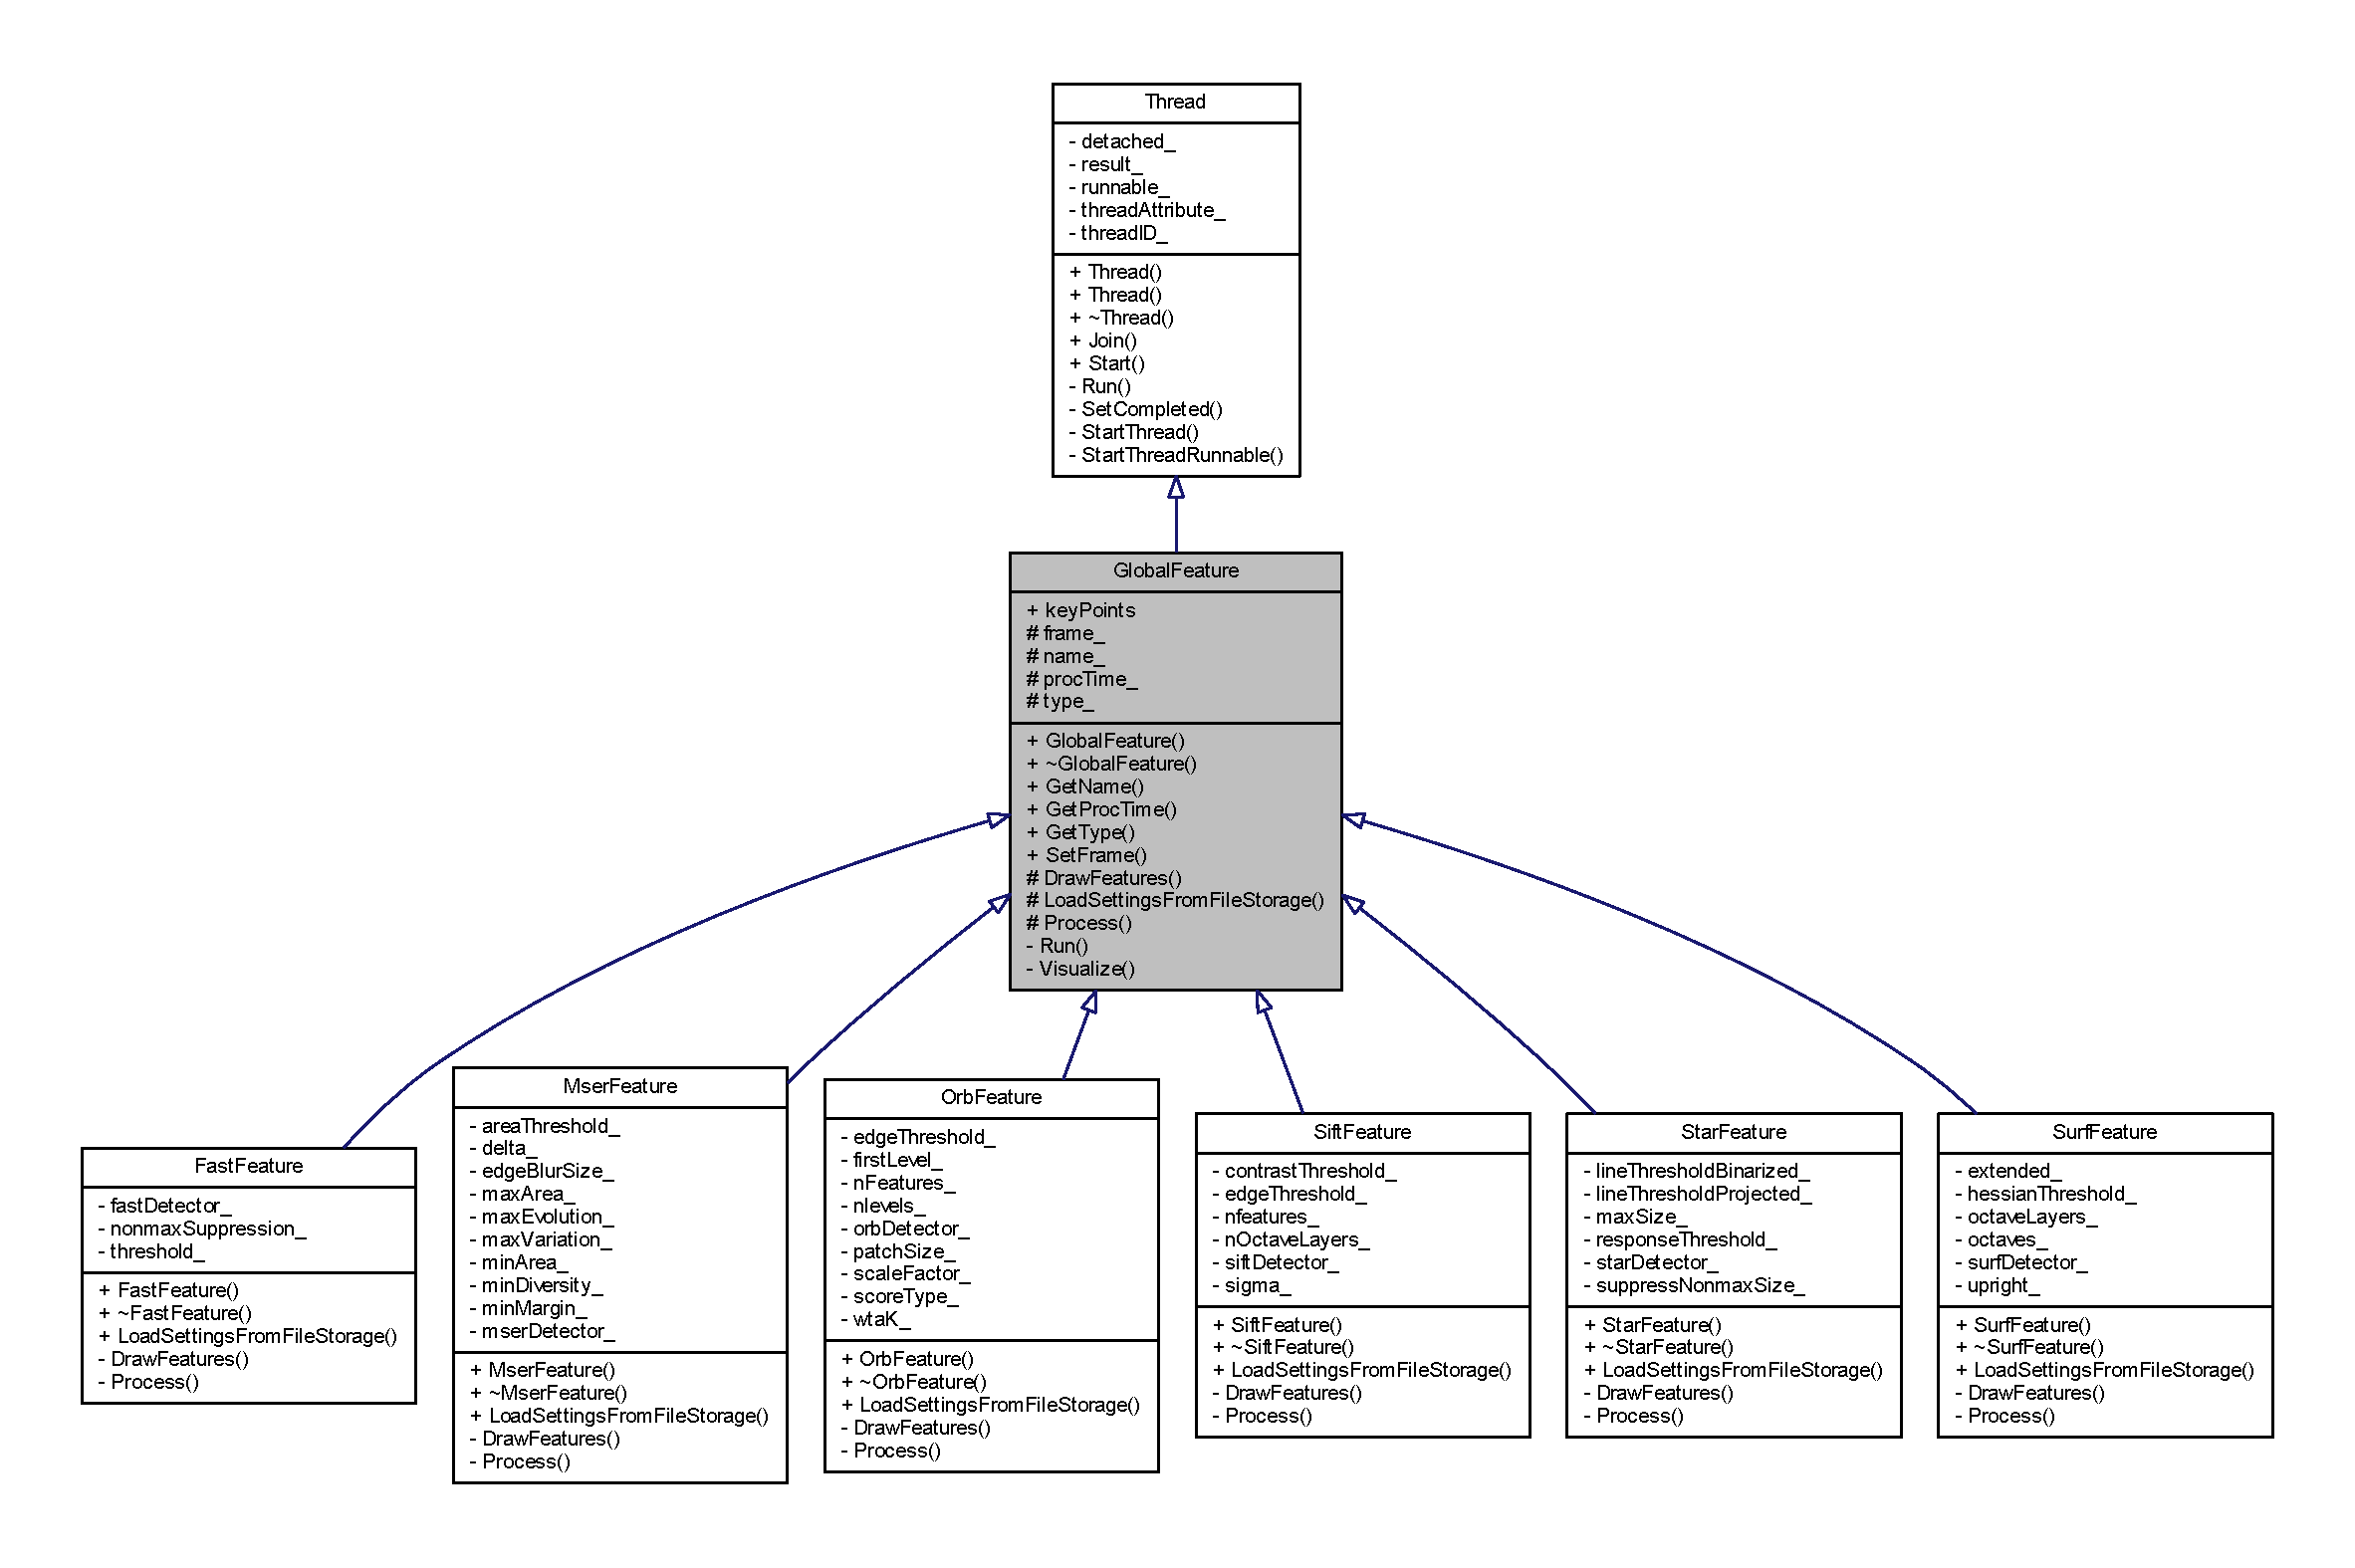
\includegraphics[width=350pt]{class_global_feature__inherit__graph}
\end{center}
\end{figure}


Collaboration diagram for Global\-Feature\-:
\nopagebreak
\begin{figure}[H]
\begin{center}
\leavevmode
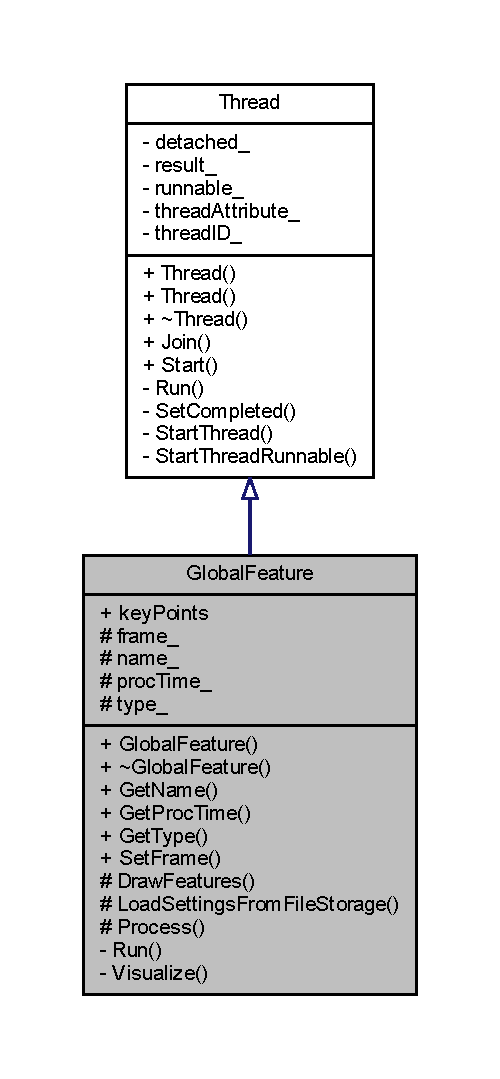
\includegraphics[width=240pt]{class_global_feature__coll__graph}
\end{center}
\end{figure}
\subsubsection*{Public Member Functions}
\begin{DoxyCompactItemize}
\item 
\hyperlink{group___feature_extractor_a835e42ce3c2d6b39189a0f2bc24afc9c}{Global\-Feature} (const std\-::string \&name, const std\-::string \&type)
\begin{DoxyCompactList}\small\item\em Constructor. \end{DoxyCompactList}\item 
\hyperlink{group___feature_extractor_a355fe3fc573a603139538394c5404832}{$\sim$\-Global\-Feature} (void)
\begin{DoxyCompactList}\small\item\em Destructor. \end{DoxyCompactList}\item 
const std\-::string \& \hyperlink{group___feature_extractor_a5f69ca2455d5eec4493dbf115d00d5c9}{Get\-Name} (void)
\begin{DoxyCompactList}\small\item\em Name getter. \end{DoxyCompactList}\item 
double \hyperlink{group___feature_extractor_ad07a3104192b50d911eee634a0be009d}{Get\-Proc\-Time} (void)
\begin{DoxyCompactList}\small\item\em Process time getter. \end{DoxyCompactList}\item 
const std\-::string \& \hyperlink{group___feature_extractor_a6724c19006d495bd6a9c8c6029236ebc}{Get\-Type} (void)
\begin{DoxyCompactList}\small\item\em Type getter. \end{DoxyCompactList}\item 
void $\ast$ \hyperlink{group___core_a8f33f7750321d5df9188033e7e3e300d}{Join} (void)
\item 
void \hyperlink{group___feature_extractor_a3c58d995fb2440b28db3b21b54b94815}{Set\-Frame} (const cv\-::\-Mat \&frame)
\begin{DoxyCompactList}\small\item\em Connects a frame to the feature extractor. \end{DoxyCompactList}\item 
void \hyperlink{group___core_a2b42f82341afd2747ea093b6ac8b91cb}{Start} (void)
\begin{DoxyCompactList}\small\item\em Starts the thread. \end{DoxyCompactList}\end{DoxyCompactItemize}
\subsubsection*{Public Attributes}
\begin{DoxyCompactItemize}
\item 
std\-::vector$<$ cv\-::\-Key\-Point $>$ \hyperlink{group___feature_extractor_a72cc606c0090a64718a7e92bca7520b9}{key\-Points}
\begin{DoxyCompactList}\small\item\em Stores keypoints, i.\-e. a point feature found by one of many available keypoint detectors. \end{DoxyCompactList}\end{DoxyCompactItemize}
\subsubsection*{Protected Member Functions}
\begin{DoxyCompactItemize}
\item 
virtual void \hyperlink{group___feature_extractor_acea1ee12c177894819ea7ae0f6294e5c}{Draw\-Features} (void)
\begin{DoxyCompactList}\small\item\em Virtual method for drawing the extracted features. \end{DoxyCompactList}\item 
virtual void \hyperlink{group___feature_extractor_aa48133762d9f52a5c2ae5042f6ebbe71}{Load\-Settings\-From\-File\-Storage} (void)
\begin{DoxyCompactList}\small\item\em Virtual method for loading algorithm specific settings from the given storage. \end{DoxyCompactList}\item 
virtual void \hyperlink{group___feature_extractor_a9fdfc934c5a9da6962ec39c1b0cf32dc}{Process} (void)
\begin{DoxyCompactList}\small\item\em Virtual method for each feature extraction algorithm. \end{DoxyCompactList}\end{DoxyCompactItemize}
\subsubsection*{Protected Attributes}
\begin{DoxyCompactItemize}
\item 
cv\-::\-Mat \hyperlink{group___feature_extractor_aae4295da2c3999edcb99b46d70ee7166}{frame\-\_\-}
\begin{DoxyCompactList}\small\item\em The current frame. \end{DoxyCompactList}\item 
std\-::string \hyperlink{group___feature_extractor_abee52be830de272bd27685083bf28aae}{name\-\_\-}
\begin{DoxyCompactList}\small\item\em Name of the current feature extraction procedure. \end{DoxyCompactList}\item 
double \hyperlink{group___feature_extractor_aa3306975b929f5503dac51829f9e04a0}{proc\-Time\-\_\-}
\begin{DoxyCompactList}\small\item\em Processing time of the current feature extraction method. \end{DoxyCompactList}\item 
std\-::string \hyperlink{group___feature_extractor_ad467857c4bc3d0fe65ba29e3b8f7c796}{type\-\_\-}
\begin{DoxyCompactList}\small\item\em Type of the current feature extraction procedure. \end{DoxyCompactList}\end{DoxyCompactItemize}
\subsubsection*{Private Member Functions}
\begin{DoxyCompactItemize}
\item 
void $\ast$ \hyperlink{group___feature_extractor_a03df7e2408a60e20a62468652c17d615}{Run} (void)
\begin{DoxyCompactList}\small\item\em Implemented virtual method for the algorithm. \end{DoxyCompactList}\item 
void \hyperlink{group___feature_extractor_aae5833316f46595edaf6dd635e391d4e}{Visualize} (void)
\begin{DoxyCompactList}\small\item\em Visualizing the output of feature extractor. \end{DoxyCompactList}\end{DoxyCompactItemize}


\paragraph{Constructor \& Destructor Documentation}
\hypertarget{group___feature_extractor_a835e42ce3c2d6b39189a0f2bc24afc9c}{\index{Global\-Feature@{Global\-Feature}!Global\-Feature@{Global\-Feature}}
\index{Global\-Feature@{Global\-Feature}!GlobalFeature@{Global\-Feature}}
\subparagraph[{Global\-Feature}]{\setlength{\rightskip}{0pt plus 5cm}Global\-Feature\-::\-Global\-Feature (
\begin{DoxyParamCaption}
\item[{const std\-::string \&}]{name, }
\item[{const std\-::string \&}]{type}
\end{DoxyParamCaption}
)}}\label{group___feature_extractor_a835e42ce3c2d6b39189a0f2bc24afc9c}


Constructor. 

\begin{DoxyVerb}    \param name Name of the current feature extraction procedure.
\end{DoxyVerb}
 
\begin{DoxyParams}{Parameters}
{\em type} & Type of the current feature extraction procedure (global or local). \\
\hline
\end{DoxyParams}
\hypertarget{group___feature_extractor_a355fe3fc573a603139538394c5404832}{\index{Global\-Feature@{Global\-Feature}!$\sim$\-Global\-Feature@{$\sim$\-Global\-Feature}}
\index{$\sim$\-Global\-Feature@{$\sim$\-Global\-Feature}!GlobalFeature@{Global\-Feature}}
\subparagraph[{$\sim$\-Global\-Feature}]{\setlength{\rightskip}{0pt plus 5cm}Global\-Feature\-::$\sim$\-Global\-Feature (
\begin{DoxyParamCaption}
\item[{void}]{}
\end{DoxyParamCaption}
)}}\label{group___feature_extractor_a355fe3fc573a603139538394c5404832}


Destructor. 



\paragraph{Member Function Documentation}
\hypertarget{group___feature_extractor_acea1ee12c177894819ea7ae0f6294e5c}{\index{Global\-Feature@{Global\-Feature}!Draw\-Features@{Draw\-Features}}
\index{Draw\-Features@{Draw\-Features}!GlobalFeature@{Global\-Feature}}
\subparagraph[{Draw\-Features}]{\setlength{\rightskip}{0pt plus 5cm}virtual void Global\-Feature\-::\-Draw\-Features (
\begin{DoxyParamCaption}
\item[{void}]{}
\end{DoxyParamCaption}
)\hspace{0.3cm}{\ttfamily [protected]}, {\ttfamily [virtual]}}}\label{group___feature_extractor_acea1ee12c177894819ea7ae0f6294e5c}


Virtual method for drawing the extracted features. 



Reimplemented in \hyperlink{group___feature_extractor_a765f433c231d5f0d088beeaa77aa0e7a}{Fast\-Feature}, \hyperlink{group___feature_extractor_a907fdd9790d0295f129f1ecdc4382031}{Orb\-Feature}, \hyperlink{group___feature_extractor_ae82e144ac3fed861dc0770cefaa828a6}{Sift\-Feature}, \hyperlink{group___feature_extractor_a2f036e794ebd63cd024dbf547765442f}{Surf\-Feature}, \hyperlink{group___feature_extractor_abed40317b412e0046df5772367d4f3dc}{Mser\-Feature}, and \hyperlink{group___feature_extractor_a6bb4f1e6808f0043707eb3c0bff1e33d}{Star\-Feature}.



Referenced by Run().



Here is the caller graph for this function\-:
\nopagebreak
\begin{figure}[H]
\begin{center}
\leavevmode
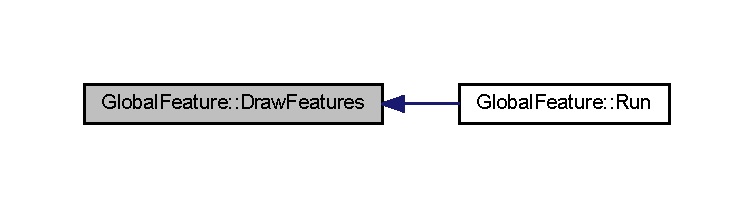
\includegraphics[width=350pt]{group___feature_extractor_acea1ee12c177894819ea7ae0f6294e5c_icgraph}
\end{center}
\end{figure}


\hypertarget{group___feature_extractor_a5f69ca2455d5eec4493dbf115d00d5c9}{\index{Global\-Feature@{Global\-Feature}!Get\-Name@{Get\-Name}}
\index{Get\-Name@{Get\-Name}!GlobalFeature@{Global\-Feature}}
\subparagraph[{Get\-Name}]{\setlength{\rightskip}{0pt plus 5cm}const string \& Global\-Feature\-::\-Get\-Name (
\begin{DoxyParamCaption}
\item[{void}]{}
\end{DoxyParamCaption}
)}}\label{group___feature_extractor_a5f69ca2455d5eec4493dbf115d00d5c9}


Name getter. 

\begin{DoxyReturn}{Returns}
Name of the current feature extraction procedure. 
\end{DoxyReturn}


References name\-\_\-.

\hypertarget{group___feature_extractor_ad07a3104192b50d911eee634a0be009d}{\index{Global\-Feature@{Global\-Feature}!Get\-Proc\-Time@{Get\-Proc\-Time}}
\index{Get\-Proc\-Time@{Get\-Proc\-Time}!GlobalFeature@{Global\-Feature}}
\subparagraph[{Get\-Proc\-Time}]{\setlength{\rightskip}{0pt plus 5cm}double Global\-Feature\-::\-Get\-Proc\-Time (
\begin{DoxyParamCaption}
\item[{void}]{}
\end{DoxyParamCaption}
)}}\label{group___feature_extractor_ad07a3104192b50d911eee634a0be009d}


Process time getter. 

\begin{DoxyReturn}{Returns}
Processing time of the current feature extraction method. 
\end{DoxyReturn}


References proc\-Time\-\_\-.

\hypertarget{group___feature_extractor_a6724c19006d495bd6a9c8c6029236ebc}{\index{Global\-Feature@{Global\-Feature}!Get\-Type@{Get\-Type}}
\index{Get\-Type@{Get\-Type}!GlobalFeature@{Global\-Feature}}
\subparagraph[{Get\-Type}]{\setlength{\rightskip}{0pt plus 5cm}const string \& Global\-Feature\-::\-Get\-Type (
\begin{DoxyParamCaption}
\item[{void}]{}
\end{DoxyParamCaption}
)}}\label{group___feature_extractor_a6724c19006d495bd6a9c8c6029236ebc}


Type getter. 

\begin{DoxyReturn}{Returns}
Type of the current feature extraction procedure. 
\end{DoxyReturn}


References type\-\_\-.

\hypertarget{group___core_a8f33f7750321d5df9188033e7e3e300d}{\index{Global\-Feature@{Global\-Feature}!Join@{Join}}
\index{Join@{Join}!GlobalFeature@{Global\-Feature}}
\subparagraph[{Join}]{\setlength{\rightskip}{0pt plus 5cm}void $\ast$ Thread\-::\-Join (
\begin{DoxyParamCaption}
\item[{void}]{}
\end{DoxyParamCaption}
)\hspace{0.3cm}{\ttfamily [inherited]}}}\label{group___core_a8f33f7750321d5df9188033e7e3e300d}


References Exception\-Error, Thread\-::result\-\_\-, and Thread\-::thread\-I\-D\-\_\-.

\hypertarget{group___feature_extractor_aa48133762d9f52a5c2ae5042f6ebbe71}{\index{Global\-Feature@{Global\-Feature}!Load\-Settings\-From\-File\-Storage@{Load\-Settings\-From\-File\-Storage}}
\index{Load\-Settings\-From\-File\-Storage@{Load\-Settings\-From\-File\-Storage}!GlobalFeature@{Global\-Feature}}
\subparagraph[{Load\-Settings\-From\-File\-Storage}]{\setlength{\rightskip}{0pt plus 5cm}virtual void Global\-Feature\-::\-Load\-Settings\-From\-File\-Storage (
\begin{DoxyParamCaption}
\item[{void}]{}
\end{DoxyParamCaption}
)\hspace{0.3cm}{\ttfamily [protected]}, {\ttfamily [virtual]}}}\label{group___feature_extractor_aa48133762d9f52a5c2ae5042f6ebbe71}


Virtual method for loading algorithm specific settings from the given storage. 



Reimplemented in \hyperlink{group___feature_extractor_a341ffc5bd43e0ee09fda3fe6f825acba}{Fast\-Feature}, \hyperlink{group___feature_extractor_aa13ad1fbc5869dcabb55611e5c206ebd}{Orb\-Feature}, \hyperlink{group___feature_extractor_af19316d789598f612ee150deb2ee5137}{Sift\-Feature}, \hyperlink{group___feature_extractor_a3717dc5d5cffd77f4f31c5ac81cd391a}{Surf\-Feature}, \hyperlink{group___feature_extractor_ae6c9bca2395a33ecac78a46e9c331979}{Mser\-Feature}, and \hyperlink{group___feature_extractor_a0a46cb80a6a4d45e324757b4ef679e81}{Star\-Feature}.

\hypertarget{group___feature_extractor_a9fdfc934c5a9da6962ec39c1b0cf32dc}{\index{Global\-Feature@{Global\-Feature}!Process@{Process}}
\index{Process@{Process}!GlobalFeature@{Global\-Feature}}
\subparagraph[{Process}]{\setlength{\rightskip}{0pt plus 5cm}virtual void Global\-Feature\-::\-Process (
\begin{DoxyParamCaption}
\item[{void}]{}
\end{DoxyParamCaption}
)\hspace{0.3cm}{\ttfamily [protected]}, {\ttfamily [virtual]}}}\label{group___feature_extractor_a9fdfc934c5a9da6962ec39c1b0cf32dc}


Virtual method for each feature extraction algorithm. 



Reimplemented in \hyperlink{group___feature_extractor_a4bbf87c97bd86bf44d4c021b053a7e66}{Fast\-Feature}, \hyperlink{group___feature_extractor_af814e3440b61e6bf13b44ef8886ad2d0}{Orb\-Feature}, \hyperlink{group___feature_extractor_a73513198ca8ff4e56be059521cfb60f5}{Sift\-Feature}, \hyperlink{group___feature_extractor_a965b300a64e776f48c1fe1564f4c4269}{Surf\-Feature}, \hyperlink{group___feature_extractor_ad96a1235b0c0df21e68c5a2742debacb}{Mser\-Feature}, and \hyperlink{group___feature_extractor_adb169936e9f60620b81894b48764a801}{Star\-Feature}.



Referenced by Run().



Here is the caller graph for this function\-:
\nopagebreak
\begin{figure}[H]
\begin{center}
\leavevmode
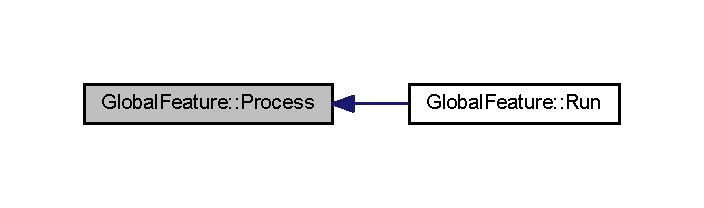
\includegraphics[width=338pt]{group___feature_extractor_a9fdfc934c5a9da6962ec39c1b0cf32dc_icgraph}
\end{center}
\end{figure}


\hypertarget{group___feature_extractor_a03df7e2408a60e20a62468652c17d615}{\index{Global\-Feature@{Global\-Feature}!Run@{Run}}
\index{Run@{Run}!GlobalFeature@{Global\-Feature}}
\subparagraph[{Run}]{\setlength{\rightskip}{0pt plus 5cm}void $\ast$ Global\-Feature\-::\-Run (
\begin{DoxyParamCaption}
\item[{void}]{}
\end{DoxyParamCaption}
)\hspace{0.3cm}{\ttfamily [private]}, {\ttfamily [virtual]}}}\label{group___feature_extractor_a03df7e2408a60e20a62468652c17d615}


Implemented virtual method for the algorithm. 

\begin{DoxySeeAlso}{See Also}
\hyperlink{group___core_ae46cda1b57e998b239a8b9710b0712e2}{Thread\-::\-Run()} 
\end{DoxySeeAlso}


Implements \hyperlink{group___core_ae46cda1b57e998b239a8b9710b0712e2}{Thread}.



References Draw\-Features(), frame\-\_\-, Process(), proc\-Time\-\_\-, and Visualize().



Here is the call graph for this function\-:
\nopagebreak
\begin{figure}[H]
\begin{center}
\leavevmode
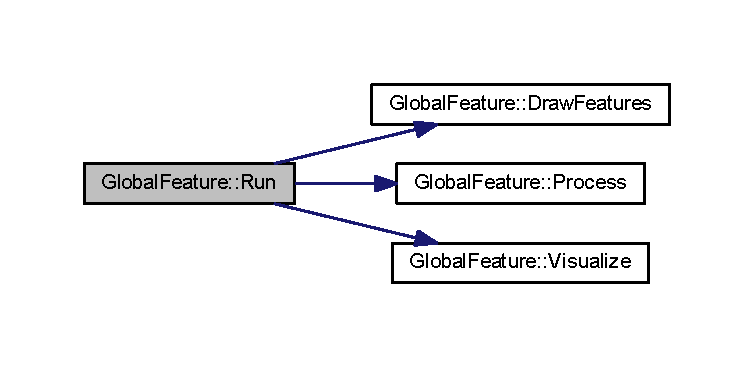
\includegraphics[width=350pt]{group___feature_extractor_a03df7e2408a60e20a62468652c17d615_cgraph}
\end{center}
\end{figure}


\hypertarget{group___feature_extractor_a3c58d995fb2440b28db3b21b54b94815}{\index{Global\-Feature@{Global\-Feature}!Set\-Frame@{Set\-Frame}}
\index{Set\-Frame@{Set\-Frame}!GlobalFeature@{Global\-Feature}}
\subparagraph[{Set\-Frame}]{\setlength{\rightskip}{0pt plus 5cm}void Global\-Feature\-::\-Set\-Frame (
\begin{DoxyParamCaption}
\item[{const cv\-::\-Mat \&}]{frame}
\end{DoxyParamCaption}
)}}\label{group___feature_extractor_a3c58d995fb2440b28db3b21b54b94815}


Connects a frame to the feature extractor. 


\begin{DoxyParams}{Parameters}
{\em frame} & Output parameter for the current frame. \\
\hline
\end{DoxyParams}


References frame\-\_\-.

\hypertarget{group___core_a2b42f82341afd2747ea093b6ac8b91cb}{\index{Global\-Feature@{Global\-Feature}!Start@{Start}}
\index{Start@{Start}!GlobalFeature@{Global\-Feature}}
\subparagraph[{Start}]{\setlength{\rightskip}{0pt plus 5cm}void Thread\-::\-Start (
\begin{DoxyParamCaption}
\item[{void}]{}
\end{DoxyParamCaption}
)\hspace{0.3cm}{\ttfamily [inherited]}}}\label{group___core_a2b42f82341afd2747ea093b6ac8b91cb}


Starts the thread. 



References Thread\-::detached\-\_\-, Exception\-Error, Thread\-::runnable\-\_\-, Thread\-::\-Start\-Thread(), Thread\-::\-Start\-Thread\-Runnable(), Thread\-::thread\-Attribute\-\_\-, and Thread\-::thread\-I\-D\-\_\-.



Here is the call graph for this function\-:
\nopagebreak
\begin{figure}[H]
\begin{center}
\leavevmode
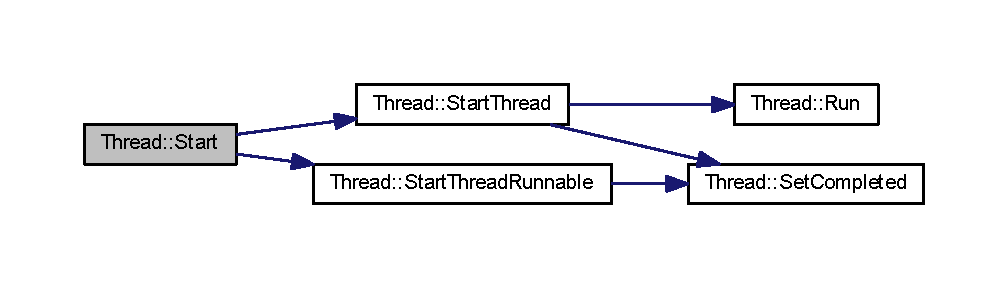
\includegraphics[width=350pt]{group___core_a2b42f82341afd2747ea093b6ac8b91cb_cgraph}
\end{center}
\end{figure}


\hypertarget{group___feature_extractor_aae5833316f46595edaf6dd635e391d4e}{\index{Global\-Feature@{Global\-Feature}!Visualize@{Visualize}}
\index{Visualize@{Visualize}!GlobalFeature@{Global\-Feature}}
\subparagraph[{Visualize}]{\setlength{\rightskip}{0pt plus 5cm}void Global\-Feature\-::\-Visualize (
\begin{DoxyParamCaption}
\item[{void}]{}
\end{DoxyParamCaption}
)\hspace{0.3cm}{\ttfamily [private]}}}\label{group___feature_extractor_aae5833316f46595edaf6dd635e391d4e}


Visualizing the output of feature extractor. 


\begin{DoxyParams}{Parameters}
{\em key\-Points\-Count} & Number of the detected keypoints. \\
\hline
\end{DoxyParams}


References frame\-\_\-, key\-Points, name\-\_\-, proc\-Time\-\_\-, and Visualizer\-Ptr.



Referenced by Run().



Here is the caller graph for this function\-:
\nopagebreak
\begin{figure}[H]
\begin{center}
\leavevmode
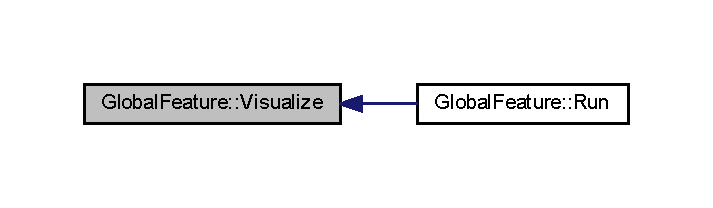
\includegraphics[width=342pt]{group___feature_extractor_aae5833316f46595edaf6dd635e391d4e_icgraph}
\end{center}
\end{figure}




\paragraph{Member Data Documentation}
\hypertarget{group___feature_extractor_aae4295da2c3999edcb99b46d70ee7166}{\index{Global\-Feature@{Global\-Feature}!frame\-\_\-@{frame\-\_\-}}
\index{frame\-\_\-@{frame\-\_\-}!GlobalFeature@{Global\-Feature}}
\subparagraph[{frame\-\_\-}]{\setlength{\rightskip}{0pt plus 5cm}cv\-::\-Mat Global\-Feature\-::frame\-\_\-\hspace{0.3cm}{\ttfamily [protected]}}}\label{group___feature_extractor_aae4295da2c3999edcb99b46d70ee7166}


The current frame. 



Referenced by Mser\-Feature\-::\-Draw\-Features(), Star\-Feature\-::\-Draw\-Features(), Sift\-Feature\-::\-Draw\-Features(), Fast\-Feature\-::\-Draw\-Features(), Orb\-Feature\-::\-Draw\-Features(), Surf\-Feature\-::\-Draw\-Features(), Mser\-Feature\-::\-Process(), Star\-Feature\-::\-Process(), Fast\-Feature\-::\-Process(), Surf\-Feature\-::\-Process(), Orb\-Feature\-::\-Process(), Sift\-Feature\-::\-Process(), Run(), Set\-Frame(), and Visualize().

\hypertarget{group___feature_extractor_a72cc606c0090a64718a7e92bca7520b9}{\index{Global\-Feature@{Global\-Feature}!key\-Points@{key\-Points}}
\index{key\-Points@{key\-Points}!GlobalFeature@{Global\-Feature}}
\subparagraph[{key\-Points}]{\setlength{\rightskip}{0pt plus 5cm}std\-::vector$<$cv\-::\-Key\-Point$>$ Global\-Feature\-::key\-Points}}\label{group___feature_extractor_a72cc606c0090a64718a7e92bca7520b9}


Stores keypoints, i.\-e. a point feature found by one of many available keypoint detectors. 



Referenced by Mser\-Feature\-::\-Draw\-Features(), Star\-Feature\-::\-Draw\-Features(), Fast\-Feature\-::\-Draw\-Features(), Orb\-Feature\-::\-Draw\-Features(), Sift\-Feature\-::\-Draw\-Features(), Surf\-Feature\-::\-Draw\-Features(), Star\-Feature\-::\-Process(), Mser\-Feature\-::\-Process(), Sift\-Feature\-::\-Process(), Fast\-Feature\-::\-Process(), Surf\-Feature\-::\-Process(), Orb\-Feature\-::\-Process(), and Visualize().

\hypertarget{group___feature_extractor_abee52be830de272bd27685083bf28aae}{\index{Global\-Feature@{Global\-Feature}!name\-\_\-@{name\-\_\-}}
\index{name\-\_\-@{name\-\_\-}!GlobalFeature@{Global\-Feature}}
\subparagraph[{name\-\_\-}]{\setlength{\rightskip}{0pt plus 5cm}std\-::string Global\-Feature\-::name\-\_\-\hspace{0.3cm}{\ttfamily [protected]}}}\label{group___feature_extractor_abee52be830de272bd27685083bf28aae}


Name of the current feature extraction procedure. 



Referenced by Get\-Name(), Mser\-Feature\-::\-Load\-Settings\-From\-File\-Storage(), Star\-Feature\-::\-Load\-Settings\-From\-File\-Storage(), Surf\-Feature\-::\-Load\-Settings\-From\-File\-Storage(), Orb\-Feature\-::\-Load\-Settings\-From\-File\-Storage(), Sift\-Feature\-::\-Load\-Settings\-From\-File\-Storage(), Fast\-Feature\-::\-Load\-Settings\-From\-File\-Storage(), and Visualize().

\hypertarget{group___feature_extractor_aa3306975b929f5503dac51829f9e04a0}{\index{Global\-Feature@{Global\-Feature}!proc\-Time\-\_\-@{proc\-Time\-\_\-}}
\index{proc\-Time\-\_\-@{proc\-Time\-\_\-}!GlobalFeature@{Global\-Feature}}
\subparagraph[{proc\-Time\-\_\-}]{\setlength{\rightskip}{0pt plus 5cm}double Global\-Feature\-::proc\-Time\-\_\-\hspace{0.3cm}{\ttfamily [protected]}}}\label{group___feature_extractor_aa3306975b929f5503dac51829f9e04a0}


Processing time of the current feature extraction method. 



Referenced by Get\-Proc\-Time(), Run(), and Visualize().

\hypertarget{group___feature_extractor_ad467857c4bc3d0fe65ba29e3b8f7c796}{\index{Global\-Feature@{Global\-Feature}!type\-\_\-@{type\-\_\-}}
\index{type\-\_\-@{type\-\_\-}!GlobalFeature@{Global\-Feature}}
\subparagraph[{type\-\_\-}]{\setlength{\rightskip}{0pt plus 5cm}std\-::string Global\-Feature\-::type\-\_\-\hspace{0.3cm}{\ttfamily [protected]}}}\label{group___feature_extractor_ad467857c4bc3d0fe65ba29e3b8f7c796}


Type of the current feature extraction procedure. 



Referenced by Get\-Type().

\index{Lbp\-Feature@{Lbp\-Feature}}\label{class_lbp_feature}
\hypertarget{group___feature_extractor_class_lbp_feature}{}
\subsubsection{class Lbp\-Feature}
Class for extracting L\-B\-P features. 

\begin{DoxyVerb}Local Binary Pattern (LBP) is a simple yet very efficient texture operator which labels the pixels of an image by thresholding the neighborhood of each pixel and considers the result as a binary number.
\end{DoxyVerb}


See paper\-: T. Ojala, M. Pietikäinen, and D. Harwood (1994), \char`\"{}\-Performance evaluation of texture measures with classification based on Kullback discrimination of distributions\char`\"{}, Proceedings of the 12th I\-A\-P\-R International Conference on Pattern Recognition (I\-C\-P\-R 1994), vol. 1, pp. 582 -\/ 585. 

Inheritance diagram for Lbp\-Feature\-:
\nopagebreak
\begin{figure}[H]
\begin{center}
\leavevmode
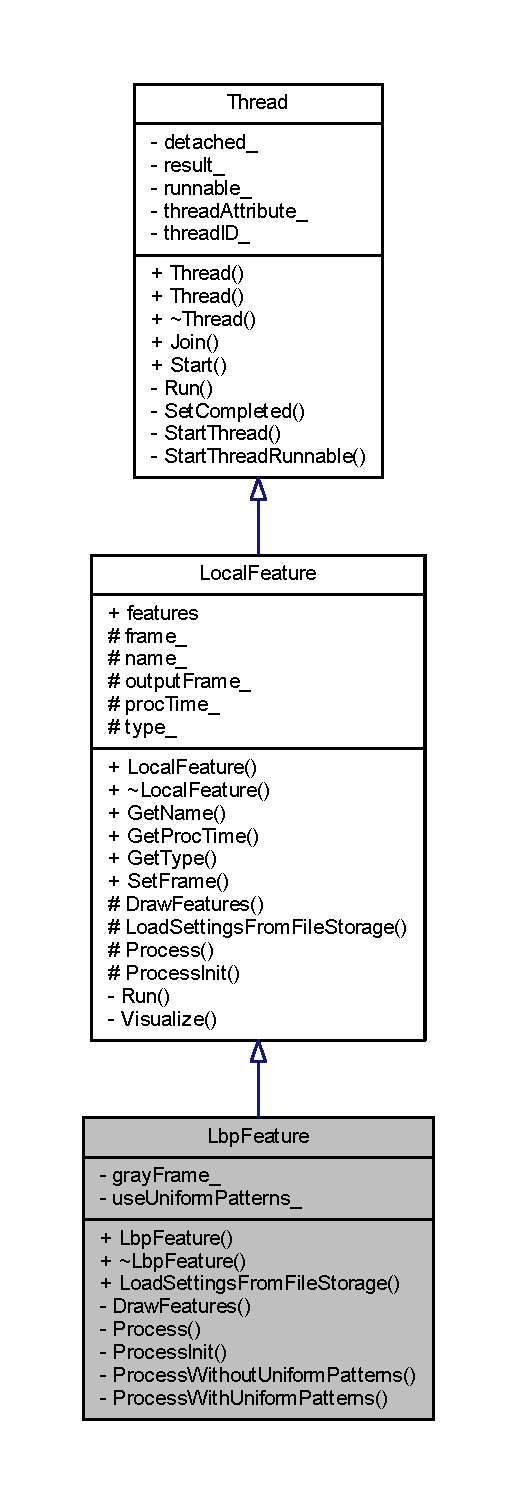
\includegraphics[height=550pt]{class_lbp_feature__inherit__graph}
\end{center}
\end{figure}


Collaboration diagram for Lbp\-Feature\-:
\nopagebreak
\begin{figure}[H]
\begin{center}
\leavevmode
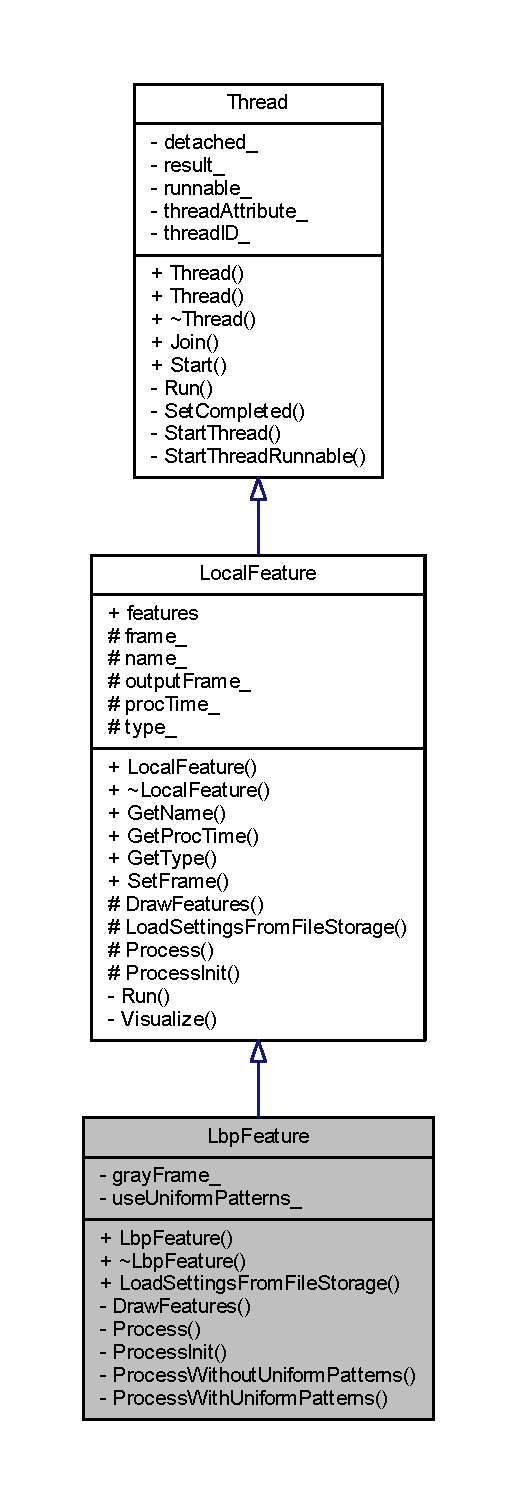
\includegraphics[height=550pt]{class_lbp_feature__coll__graph}
\end{center}
\end{figure}
\subsubsection*{Public Member Functions}
\begin{DoxyCompactItemize}
\item 
\hyperlink{group___feature_extractor_a52b160f5fa16bc1ea0c489a744ed554f}{Lbp\-Feature} (const std\-::string \&name, const std\-::string \&type)
\begin{DoxyCompactList}\small\item\em Constructor. \end{DoxyCompactList}\item 
\hyperlink{group___feature_extractor_a40826a6cc5bc5f1de7edf8b05092052b}{$\sim$\-Lbp\-Feature} (void)
\begin{DoxyCompactList}\small\item\em Destructor. \end{DoxyCompactList}\item 
const std\-::string \& \hyperlink{group___feature_extractor_ab2ecc77360b2fa1400f29298a8e1b751}{Get\-Name} (void)
\begin{DoxyCompactList}\small\item\em Name getter. \end{DoxyCompactList}\item 
double \hyperlink{group___feature_extractor_a46f41fabf78e63d9e9c93cbaadf652a1}{Get\-Proc\-Time} (void)
\begin{DoxyCompactList}\small\item\em Process time getter. \end{DoxyCompactList}\item 
const std\-::string \& \hyperlink{group___feature_extractor_aba5fb3207f97ae73dc3cab7572baf85e}{Get\-Type} (void)
\begin{DoxyCompactList}\small\item\em Type getter. \end{DoxyCompactList}\item 
void $\ast$ \hyperlink{group___core_a8f33f7750321d5df9188033e7e3e300d}{Join} (void)
\item 
void \hyperlink{group___feature_extractor_a39ac99c8b8537ac9d104ae4368177071}{Load\-Settings\-From\-File\-Storage} (void)
\begin{DoxyCompactList}\small\item\em Implemented virtual method for loading algorithm specific settings from the given storage. \end{DoxyCompactList}\item 
void \hyperlink{group___feature_extractor_aee5c4e09e373308e7f50bfaffd8e2267}{Set\-Frame} (const cv\-::\-Mat \&frame)
\begin{DoxyCompactList}\small\item\em Connects a frame to the feature extractor. \end{DoxyCompactList}\item 
void \hyperlink{group___core_a2b42f82341afd2747ea093b6ac8b91cb}{Start} (void)
\begin{DoxyCompactList}\small\item\em Starts the thread. \end{DoxyCompactList}\end{DoxyCompactItemize}
\subsubsection*{Public Attributes}
\begin{DoxyCompactItemize}
\item 
std\-::vector$<$ double $>$ \hyperlink{group___feature_extractor_a8197cec0d029bac380885167df9f65e5}{features}
\begin{DoxyCompactList}\small\item\em Stores local features. \end{DoxyCompactList}\end{DoxyCompactItemize}
\subsubsection*{Protected Attributes}
\begin{DoxyCompactItemize}
\item 
cv\-::\-Mat \hyperlink{group___feature_extractor_a585b0dc6e6184422c5563e80bff50ffa}{frame\-\_\-}
\begin{DoxyCompactList}\small\item\em The current frame. \end{DoxyCompactList}\item 
std\-::string \hyperlink{group___feature_extractor_a0e73ef0aed82c04f06b6eeb9a9b9be8b}{name\-\_\-}
\begin{DoxyCompactList}\small\item\em Name of the current feature extraction procedure. \end{DoxyCompactList}\item 
cv\-::\-Mat \hyperlink{group___feature_extractor_a1c7b8087feb05f02b09eb1b536d443e6}{output\-Frame\-\_\-}
\begin{DoxyCompactList}\small\item\em The current frame. \end{DoxyCompactList}\item 
double \hyperlink{group___feature_extractor_a79d60ce90ab8e6ccd66ff8f7da2365c7}{proc\-Time\-\_\-}
\begin{DoxyCompactList}\small\item\em Processing time of the current feature extraction method. \end{DoxyCompactList}\item 
std\-::string \hyperlink{group___feature_extractor_aaf3aef30088cd1be80e1770d0a9d945b}{type\-\_\-}
\begin{DoxyCompactList}\small\item\em Type of the current feature extraction procedure. \end{DoxyCompactList}\end{DoxyCompactItemize}
\subsubsection*{Private Member Functions}
\begin{DoxyCompactItemize}
\item 
void \hyperlink{group___feature_extractor_a152c1785ca51eb7e5878c0d3f9309697}{Draw\-Features} (void)
\begin{DoxyCompactList}\small\item\em Implemented virtual method for displaying the output. \end{DoxyCompactList}\item 
void \hyperlink{group___feature_extractor_af664c189044d32f2cb71b334deb6f0c7}{Process} (void)
\begin{DoxyCompactList}\small\item\em Implemented virtual method for the algorithm. \end{DoxyCompactList}\item 
void \hyperlink{group___feature_extractor_a773b1c3fd663f58b01f1ba33a897744f}{Process\-Init} (void)
\begin{DoxyCompactList}\small\item\em Initalizing the variables. \end{DoxyCompactList}\item 
void \hyperlink{group___feature_extractor_a96e42213e77e729c263236db12453bde}{Process\-Without\-Uniform\-Patterns} (void)
\begin{DoxyCompactList}\small\item\em Generate feature vector without using uniform patterns. \end{DoxyCompactList}\item 
void \hyperlink{group___feature_extractor_aa29955bd43f95dcac63aa7840fcd1925}{Process\-With\-Uniform\-Patterns} (void)
\begin{DoxyCompactList}\small\item\em Generate feature vector with using uniform patterns. \end{DoxyCompactList}\end{DoxyCompactItemize}
\subsubsection*{Private Attributes}
\begin{DoxyCompactItemize}
\item 
cv\-::\-Mat \hyperlink{group___feature_extractor_ab2bdc329e16e4126eccbbe4b8d4d44f5}{gray\-Frame\-\_\-}
\item 
bool \hyperlink{group___feature_extractor_a6025f411377d4b6e56aa9eb5daff07e8}{use\-Uniform\-Patterns\-\_\-}
\end{DoxyCompactItemize}


\paragraph{Constructor \& Destructor Documentation}
\hypertarget{group___feature_extractor_a52b160f5fa16bc1ea0c489a744ed554f}{\index{Lbp\-Feature@{Lbp\-Feature}!Lbp\-Feature@{Lbp\-Feature}}
\index{Lbp\-Feature@{Lbp\-Feature}!LbpFeature@{Lbp\-Feature}}
\subparagraph[{Lbp\-Feature}]{\setlength{\rightskip}{0pt plus 5cm}Lbp\-Feature\-::\-Lbp\-Feature (
\begin{DoxyParamCaption}
\item[{const std\-::string \&}]{name, }
\item[{const std\-::string \&}]{type}
\end{DoxyParamCaption}
)}}\label{group___feature_extractor_a52b160f5fa16bc1ea0c489a744ed554f}


Constructor. 

\begin{DoxyVerb}    \param name Name of the current feature extraction procedure.
\end{DoxyVerb}
 
\begin{DoxyParams}{Parameters}
{\em type} & Type of the current feature extraction procedure (global or local). \\
\hline
\end{DoxyParams}


References Load\-Settings\-From\-File\-Storage().



Here is the call graph for this function\-:
\nopagebreak
\begin{figure}[H]
\begin{center}
\leavevmode
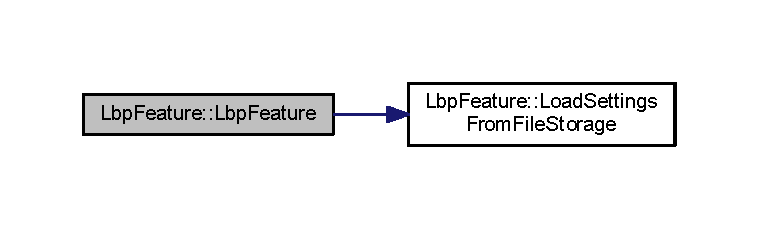
\includegraphics[width=350pt]{group___feature_extractor_a52b160f5fa16bc1ea0c489a744ed554f_cgraph}
\end{center}
\end{figure}


\hypertarget{group___feature_extractor_a40826a6cc5bc5f1de7edf8b05092052b}{\index{Lbp\-Feature@{Lbp\-Feature}!$\sim$\-Lbp\-Feature@{$\sim$\-Lbp\-Feature}}
\index{$\sim$\-Lbp\-Feature@{$\sim$\-Lbp\-Feature}!LbpFeature@{Lbp\-Feature}}
\subparagraph[{$\sim$\-Lbp\-Feature}]{\setlength{\rightskip}{0pt plus 5cm}Lbp\-Feature\-::$\sim$\-Lbp\-Feature (
\begin{DoxyParamCaption}
\item[{void}]{}
\end{DoxyParamCaption}
)}}\label{group___feature_extractor_a40826a6cc5bc5f1de7edf8b05092052b}


Destructor. 



\paragraph{Member Function Documentation}
\hypertarget{group___feature_extractor_a152c1785ca51eb7e5878c0d3f9309697}{\index{Lbp\-Feature@{Lbp\-Feature}!Draw\-Features@{Draw\-Features}}
\index{Draw\-Features@{Draw\-Features}!LbpFeature@{Lbp\-Feature}}
\subparagraph[{Draw\-Features}]{\setlength{\rightskip}{0pt plus 5cm}void Lbp\-Feature\-::\-Draw\-Features (
\begin{DoxyParamCaption}
\item[{void}]{}
\end{DoxyParamCaption}
)\hspace{0.3cm}{\ttfamily [private]}, {\ttfamily [virtual]}}}\label{group___feature_extractor_a152c1785ca51eb7e5878c0d3f9309697}


Implemented virtual method for displaying the output. 

\begin{DoxySeeAlso}{See Also}
\hyperlink{group___feature_extractor_a329c560d8f02a4ab390716319410deab}{Local\-Feature\-::\-Draw\-Features()} 
\end{DoxySeeAlso}


Reimplemented from \hyperlink{group___feature_extractor_a329c560d8f02a4ab390716319410deab}{Local\-Feature}.

\hypertarget{group___feature_extractor_ab2ecc77360b2fa1400f29298a8e1b751}{\index{Lbp\-Feature@{Lbp\-Feature}!Get\-Name@{Get\-Name}}
\index{Get\-Name@{Get\-Name}!LbpFeature@{Lbp\-Feature}}
\subparagraph[{Get\-Name}]{\setlength{\rightskip}{0pt plus 5cm}const string \& Local\-Feature\-::\-Get\-Name (
\begin{DoxyParamCaption}
\item[{void}]{}
\end{DoxyParamCaption}
)\hspace{0.3cm}{\ttfamily [inherited]}}}\label{group___feature_extractor_ab2ecc77360b2fa1400f29298a8e1b751}


Name getter. 

\begin{DoxyReturn}{Returns}
Name of the current feature extraction procedure. 
\end{DoxyReturn}


References Local\-Feature\-::name\-\_\-.

\hypertarget{group___feature_extractor_a46f41fabf78e63d9e9c93cbaadf652a1}{\index{Lbp\-Feature@{Lbp\-Feature}!Get\-Proc\-Time@{Get\-Proc\-Time}}
\index{Get\-Proc\-Time@{Get\-Proc\-Time}!LbpFeature@{Lbp\-Feature}}
\subparagraph[{Get\-Proc\-Time}]{\setlength{\rightskip}{0pt plus 5cm}double Local\-Feature\-::\-Get\-Proc\-Time (
\begin{DoxyParamCaption}
\item[{void}]{}
\end{DoxyParamCaption}
)\hspace{0.3cm}{\ttfamily [inherited]}}}\label{group___feature_extractor_a46f41fabf78e63d9e9c93cbaadf652a1}


Process time getter. 

\begin{DoxyReturn}{Returns}
Processing time of the current feature extraction method. 
\end{DoxyReturn}


References Local\-Feature\-::proc\-Time\-\_\-.

\hypertarget{group___feature_extractor_aba5fb3207f97ae73dc3cab7572baf85e}{\index{Lbp\-Feature@{Lbp\-Feature}!Get\-Type@{Get\-Type}}
\index{Get\-Type@{Get\-Type}!LbpFeature@{Lbp\-Feature}}
\subparagraph[{Get\-Type}]{\setlength{\rightskip}{0pt plus 5cm}const string \& Local\-Feature\-::\-Get\-Type (
\begin{DoxyParamCaption}
\item[{void}]{}
\end{DoxyParamCaption}
)\hspace{0.3cm}{\ttfamily [inherited]}}}\label{group___feature_extractor_aba5fb3207f97ae73dc3cab7572baf85e}


Type getter. 

\begin{DoxyReturn}{Returns}
Type of the current feature extraction procedure. 
\end{DoxyReturn}


References Local\-Feature\-::type\-\_\-.

\hypertarget{group___core_a8f33f7750321d5df9188033e7e3e300d}{\index{Lbp\-Feature@{Lbp\-Feature}!Join@{Join}}
\index{Join@{Join}!LbpFeature@{Lbp\-Feature}}
\subparagraph[{Join}]{\setlength{\rightskip}{0pt plus 5cm}void $\ast$ Thread\-::\-Join (
\begin{DoxyParamCaption}
\item[{void}]{}
\end{DoxyParamCaption}
)\hspace{0.3cm}{\ttfamily [inherited]}}}\label{group___core_a8f33f7750321d5df9188033e7e3e300d}


References Exception\-Error, Thread\-::result\-\_\-, and Thread\-::thread\-I\-D\-\_\-.

\hypertarget{group___feature_extractor_a39ac99c8b8537ac9d104ae4368177071}{\index{Lbp\-Feature@{Lbp\-Feature}!Load\-Settings\-From\-File\-Storage@{Load\-Settings\-From\-File\-Storage}}
\index{Load\-Settings\-From\-File\-Storage@{Load\-Settings\-From\-File\-Storage}!LbpFeature@{Lbp\-Feature}}
\subparagraph[{Load\-Settings\-From\-File\-Storage}]{\setlength{\rightskip}{0pt plus 5cm}void Lbp\-Feature\-::\-Load\-Settings\-From\-File\-Storage (
\begin{DoxyParamCaption}
\item[{void}]{}
\end{DoxyParamCaption}
)\hspace{0.3cm}{\ttfamily [virtual]}}}\label{group___feature_extractor_a39ac99c8b8537ac9d104ae4368177071}


Implemented virtual method for loading algorithm specific settings from the given storage. 

\begin{DoxySeeAlso}{See Also}
Feature\-::\-Load\-Settings\-From\-File\-Storage() 
\end{DoxySeeAlso}


Reimplemented from \hyperlink{group___feature_extractor_a9280742c803d38c984121a33cdd67723}{Local\-Feature}.



References Exception\-Error, Local\-Settings\-Ptr, Local\-Feature\-::name\-\_\-, and use\-Uniform\-Patterns\-\_\-.



Referenced by Lbp\-Feature().



Here is the caller graph for this function\-:
\nopagebreak
\begin{figure}[H]
\begin{center}
\leavevmode
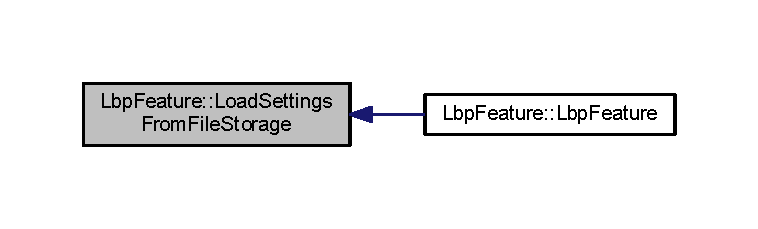
\includegraphics[width=350pt]{group___feature_extractor_a39ac99c8b8537ac9d104ae4368177071_icgraph}
\end{center}
\end{figure}


\hypertarget{group___feature_extractor_af664c189044d32f2cb71b334deb6f0c7}{\index{Lbp\-Feature@{Lbp\-Feature}!Process@{Process}}
\index{Process@{Process}!LbpFeature@{Lbp\-Feature}}
\subparagraph[{Process}]{\setlength{\rightskip}{0pt plus 5cm}void Lbp\-Feature\-::\-Process (
\begin{DoxyParamCaption}
\item[{void}]{}
\end{DoxyParamCaption}
)\hspace{0.3cm}{\ttfamily [private]}, {\ttfamily [virtual]}}}\label{group___feature_extractor_af664c189044d32f2cb71b334deb6f0c7}


Implemented virtual method for the algorithm. 

\begin{DoxySeeAlso}{See Also}
\hyperlink{group___feature_extractor_a2f5b230fd63be9c1dcceb51361bc6ee1}{Local\-Feature\-::\-Process()} 
\end{DoxySeeAlso}


Reimplemented from \hyperlink{group___feature_extractor_a2f5b230fd63be9c1dcceb51361bc6ee1}{Local\-Feature}.



References Local\-Feature\-::features, Local\-Feature\-::frame\-\_\-, Process\-Without\-Uniform\-Patterns(), Process\-With\-Uniform\-Patterns(), and use\-Uniform\-Patterns\-\_\-.



Here is the call graph for this function\-:
\nopagebreak
\begin{figure}[H]
\begin{center}
\leavevmode
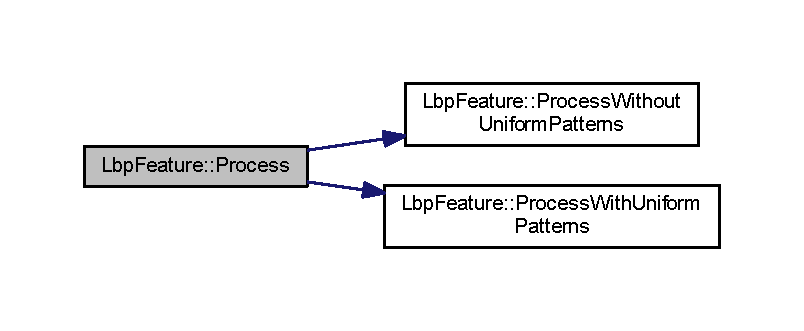
\includegraphics[width=350pt]{group___feature_extractor_af664c189044d32f2cb71b334deb6f0c7_cgraph}
\end{center}
\end{figure}


\hypertarget{group___feature_extractor_a773b1c3fd663f58b01f1ba33a897744f}{\index{Lbp\-Feature@{Lbp\-Feature}!Process\-Init@{Process\-Init}}
\index{Process\-Init@{Process\-Init}!LbpFeature@{Lbp\-Feature}}
\subparagraph[{Process\-Init}]{\setlength{\rightskip}{0pt plus 5cm}void Lbp\-Feature\-::\-Process\-Init (
\begin{DoxyParamCaption}
\item[{void}]{}
\end{DoxyParamCaption}
)\hspace{0.3cm}{\ttfamily [private]}, {\ttfamily [virtual]}}}\label{group___feature_extractor_a773b1c3fd663f58b01f1ba33a897744f}


Initalizing the variables. 

\begin{DoxySeeAlso}{See Also}
\hyperlink{group___feature_extractor_a2b2cdc0b1be48785e967a87c268ee27e}{Local\-Feature\-::\-Process\-Init()} 
\end{DoxySeeAlso}


Reimplemented from \hyperlink{group___feature_extractor_a2b2cdc0b1be48785e967a87c268ee27e}{Local\-Feature}.



References Local\-Feature\-::frame\-\_\-, gray\-Frame\-\_\-, and Local\-Feature\-::output\-Frame\-\_\-.

\hypertarget{group___feature_extractor_a96e42213e77e729c263236db12453bde}{\index{Lbp\-Feature@{Lbp\-Feature}!Process\-Without\-Uniform\-Patterns@{Process\-Without\-Uniform\-Patterns}}
\index{Process\-Without\-Uniform\-Patterns@{Process\-Without\-Uniform\-Patterns}!LbpFeature@{Lbp\-Feature}}
\subparagraph[{Process\-Without\-Uniform\-Patterns}]{\setlength{\rightskip}{0pt plus 5cm}void Lbp\-Feature\-::\-Process\-Without\-Uniform\-Patterns (
\begin{DoxyParamCaption}
\item[{void}]{}
\end{DoxyParamCaption}
)\hspace{0.3cm}{\ttfamily [private]}}}\label{group___feature_extractor_a96e42213e77e729c263236db12453bde}


Generate feature vector without using uniform patterns. 



References Local\-Feature\-::features, Local\-Feature\-::frame\-\_\-, gray\-Frame\-\_\-, and Local\-Feature\-::output\-Frame\-\_\-.



Referenced by Process().



Here is the caller graph for this function\-:
\nopagebreak
\begin{figure}[H]
\begin{center}
\leavevmode
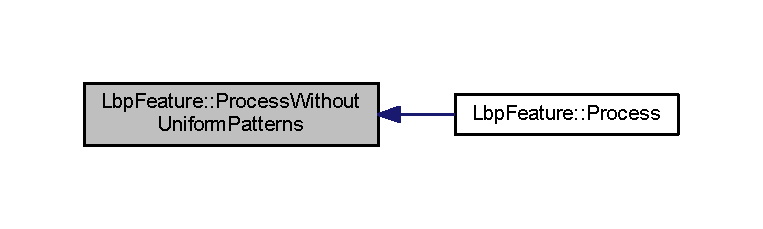
\includegraphics[width=350pt]{group___feature_extractor_a96e42213e77e729c263236db12453bde_icgraph}
\end{center}
\end{figure}


\hypertarget{group___feature_extractor_aa29955bd43f95dcac63aa7840fcd1925}{\index{Lbp\-Feature@{Lbp\-Feature}!Process\-With\-Uniform\-Patterns@{Process\-With\-Uniform\-Patterns}}
\index{Process\-With\-Uniform\-Patterns@{Process\-With\-Uniform\-Patterns}!LbpFeature@{Lbp\-Feature}}
\subparagraph[{Process\-With\-Uniform\-Patterns}]{\setlength{\rightskip}{0pt plus 5cm}void Lbp\-Feature\-::\-Process\-With\-Uniform\-Patterns (
\begin{DoxyParamCaption}
\item[{void}]{}
\end{DoxyParamCaption}
)\hspace{0.3cm}{\ttfamily [private]}}}\label{group___feature_extractor_aa29955bd43f95dcac63aa7840fcd1925}


Generate feature vector with using uniform patterns. 



References Local\-Feature\-::features, Local\-Feature\-::frame\-\_\-, gray\-Frame\-\_\-, and Local\-Feature\-::output\-Frame\-\_\-.



Referenced by Process().



Here is the caller graph for this function\-:
\nopagebreak
\begin{figure}[H]
\begin{center}
\leavevmode
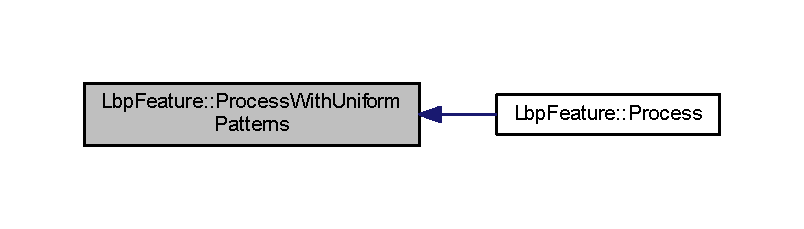
\includegraphics[width=350pt]{group___feature_extractor_aa29955bd43f95dcac63aa7840fcd1925_icgraph}
\end{center}
\end{figure}


\hypertarget{group___feature_extractor_aee5c4e09e373308e7f50bfaffd8e2267}{\index{Lbp\-Feature@{Lbp\-Feature}!Set\-Frame@{Set\-Frame}}
\index{Set\-Frame@{Set\-Frame}!LbpFeature@{Lbp\-Feature}}
\subparagraph[{Set\-Frame}]{\setlength{\rightskip}{0pt plus 5cm}void Local\-Feature\-::\-Set\-Frame (
\begin{DoxyParamCaption}
\item[{const cv\-::\-Mat \&}]{frame}
\end{DoxyParamCaption}
)\hspace{0.3cm}{\ttfamily [inherited]}}}\label{group___feature_extractor_aee5c4e09e373308e7f50bfaffd8e2267}


Connects a frame to the feature extractor. 


\begin{DoxyParams}{Parameters}
{\em frame} & Output parameter for the current frame. \\
\hline
\end{DoxyParams}


References Local\-Feature\-::frame\-\_\-.

\hypertarget{group___core_a2b42f82341afd2747ea093b6ac8b91cb}{\index{Lbp\-Feature@{Lbp\-Feature}!Start@{Start}}
\index{Start@{Start}!LbpFeature@{Lbp\-Feature}}
\subparagraph[{Start}]{\setlength{\rightskip}{0pt plus 5cm}void Thread\-::\-Start (
\begin{DoxyParamCaption}
\item[{void}]{}
\end{DoxyParamCaption}
)\hspace{0.3cm}{\ttfamily [inherited]}}}\label{group___core_a2b42f82341afd2747ea093b6ac8b91cb}


Starts the thread. 



References Thread\-::detached\-\_\-, Exception\-Error, Thread\-::runnable\-\_\-, Thread\-::\-Start\-Thread(), Thread\-::\-Start\-Thread\-Runnable(), Thread\-::thread\-Attribute\-\_\-, and Thread\-::thread\-I\-D\-\_\-.



Here is the call graph for this function\-:
\nopagebreak
\begin{figure}[H]
\begin{center}
\leavevmode
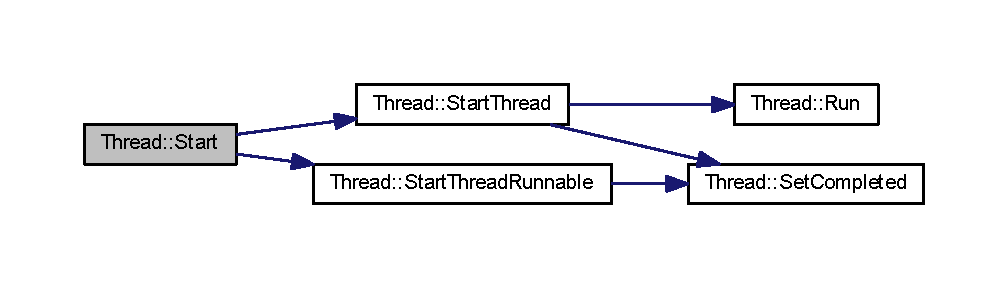
\includegraphics[width=350pt]{group___core_a2b42f82341afd2747ea093b6ac8b91cb_cgraph}
\end{center}
\end{figure}




\paragraph{Member Data Documentation}
\hypertarget{group___feature_extractor_a8197cec0d029bac380885167df9f65e5}{\index{Lbp\-Feature@{Lbp\-Feature}!features@{features}}
\index{features@{features}!LbpFeature@{Lbp\-Feature}}
\subparagraph[{features}]{\setlength{\rightskip}{0pt plus 5cm}std\-::vector$<$double$>$ Local\-Feature\-::features\hspace{0.3cm}{\ttfamily [inherited]}}}\label{group___feature_extractor_a8197cec0d029bac380885167df9f65e5}


Stores local features. 



Referenced by Process(), Process\-Without\-Uniform\-Patterns(), Process\-With\-Uniform\-Patterns(), and Local\-Feature\-::\-Visualize().

\hypertarget{group___feature_extractor_a585b0dc6e6184422c5563e80bff50ffa}{\index{Lbp\-Feature@{Lbp\-Feature}!frame\-\_\-@{frame\-\_\-}}
\index{frame\-\_\-@{frame\-\_\-}!LbpFeature@{Lbp\-Feature}}
\subparagraph[{frame\-\_\-}]{\setlength{\rightskip}{0pt plus 5cm}cv\-::\-Mat Local\-Feature\-::frame\-\_\-\hspace{0.3cm}{\ttfamily [protected]}, {\ttfamily [inherited]}}}\label{group___feature_extractor_a585b0dc6e6184422c5563e80bff50ffa}


The current frame. 



Referenced by Process(), Process\-Init(), Process\-Without\-Uniform\-Patterns(), Process\-With\-Uniform\-Patterns(), Local\-Feature\-::\-Run(), and Local\-Feature\-::\-Set\-Frame().

\hypertarget{group___feature_extractor_ab2bdc329e16e4126eccbbe4b8d4d44f5}{\index{Lbp\-Feature@{Lbp\-Feature}!gray\-Frame\-\_\-@{gray\-Frame\-\_\-}}
\index{gray\-Frame\-\_\-@{gray\-Frame\-\_\-}!LbpFeature@{Lbp\-Feature}}
\subparagraph[{gray\-Frame\-\_\-}]{\setlength{\rightskip}{0pt plus 5cm}cv\-::\-Mat Lbp\-Feature\-::gray\-Frame\-\_\-\hspace{0.3cm}{\ttfamily [private]}}}\label{group___feature_extractor_ab2bdc329e16e4126eccbbe4b8d4d44f5}


Referenced by Process\-Init(), Process\-Without\-Uniform\-Patterns(), and Process\-With\-Uniform\-Patterns().

\hypertarget{group___feature_extractor_a0e73ef0aed82c04f06b6eeb9a9b9be8b}{\index{Lbp\-Feature@{Lbp\-Feature}!name\-\_\-@{name\-\_\-}}
\index{name\-\_\-@{name\-\_\-}!LbpFeature@{Lbp\-Feature}}
\subparagraph[{name\-\_\-}]{\setlength{\rightskip}{0pt plus 5cm}std\-::string Local\-Feature\-::name\-\_\-\hspace{0.3cm}{\ttfamily [protected]}, {\ttfamily [inherited]}}}\label{group___feature_extractor_a0e73ef0aed82c04f06b6eeb9a9b9be8b}


Name of the current feature extraction procedure. 



Referenced by Local\-Feature\-::\-Get\-Name(), Load\-Settings\-From\-File\-Storage(), and Local\-Feature\-::\-Visualize().

\hypertarget{group___feature_extractor_a1c7b8087feb05f02b09eb1b536d443e6}{\index{Lbp\-Feature@{Lbp\-Feature}!output\-Frame\-\_\-@{output\-Frame\-\_\-}}
\index{output\-Frame\-\_\-@{output\-Frame\-\_\-}!LbpFeature@{Lbp\-Feature}}
\subparagraph[{output\-Frame\-\_\-}]{\setlength{\rightskip}{0pt plus 5cm}cv\-::\-Mat Local\-Feature\-::output\-Frame\-\_\-\hspace{0.3cm}{\ttfamily [protected]}, {\ttfamily [inherited]}}}\label{group___feature_extractor_a1c7b8087feb05f02b09eb1b536d443e6}


The current frame. 



Referenced by Process\-Init(), Process\-Without\-Uniform\-Patterns(), Process\-With\-Uniform\-Patterns(), and Local\-Feature\-::\-Visualize().

\hypertarget{group___feature_extractor_a79d60ce90ab8e6ccd66ff8f7da2365c7}{\index{Lbp\-Feature@{Lbp\-Feature}!proc\-Time\-\_\-@{proc\-Time\-\_\-}}
\index{proc\-Time\-\_\-@{proc\-Time\-\_\-}!LbpFeature@{Lbp\-Feature}}
\subparagraph[{proc\-Time\-\_\-}]{\setlength{\rightskip}{0pt plus 5cm}double Local\-Feature\-::proc\-Time\-\_\-\hspace{0.3cm}{\ttfamily [protected]}, {\ttfamily [inherited]}}}\label{group___feature_extractor_a79d60ce90ab8e6ccd66ff8f7da2365c7}


Processing time of the current feature extraction method. 



Referenced by Local\-Feature\-::\-Get\-Proc\-Time(), Local\-Feature\-::\-Run(), and Local\-Feature\-::\-Visualize().

\hypertarget{group___feature_extractor_aaf3aef30088cd1be80e1770d0a9d945b}{\index{Lbp\-Feature@{Lbp\-Feature}!type\-\_\-@{type\-\_\-}}
\index{type\-\_\-@{type\-\_\-}!LbpFeature@{Lbp\-Feature}}
\subparagraph[{type\-\_\-}]{\setlength{\rightskip}{0pt plus 5cm}std\-::string Local\-Feature\-::type\-\_\-\hspace{0.3cm}{\ttfamily [protected]}, {\ttfamily [inherited]}}}\label{group___feature_extractor_aaf3aef30088cd1be80e1770d0a9d945b}


Type of the current feature extraction procedure. 



Referenced by Local\-Feature\-::\-Get\-Type().

\hypertarget{group___feature_extractor_a6025f411377d4b6e56aa9eb5daff07e8}{\index{Lbp\-Feature@{Lbp\-Feature}!use\-Uniform\-Patterns\-\_\-@{use\-Uniform\-Patterns\-\_\-}}
\index{use\-Uniform\-Patterns\-\_\-@{use\-Uniform\-Patterns\-\_\-}!LbpFeature@{Lbp\-Feature}}
\subparagraph[{use\-Uniform\-Patterns\-\_\-}]{\setlength{\rightskip}{0pt plus 5cm}bool Lbp\-Feature\-::use\-Uniform\-Patterns\-\_\-\hspace{0.3cm}{\ttfamily [private]}}}\label{group___feature_extractor_a6025f411377d4b6e56aa9eb5daff07e8}


Referenced by Load\-Settings\-From\-File\-Storage(), and Process().

\index{Local\-Feature@{Local\-Feature}}\label{class_local_feature}
\hypertarget{group___feature_extractor_class_local_feature}{}
\subsubsection{class Local\-Feature}
Abstract class for local feature extraction. 

Inheritance diagram for Local\-Feature\-:
\nopagebreak
\begin{figure}[H]
\begin{center}
\leavevmode
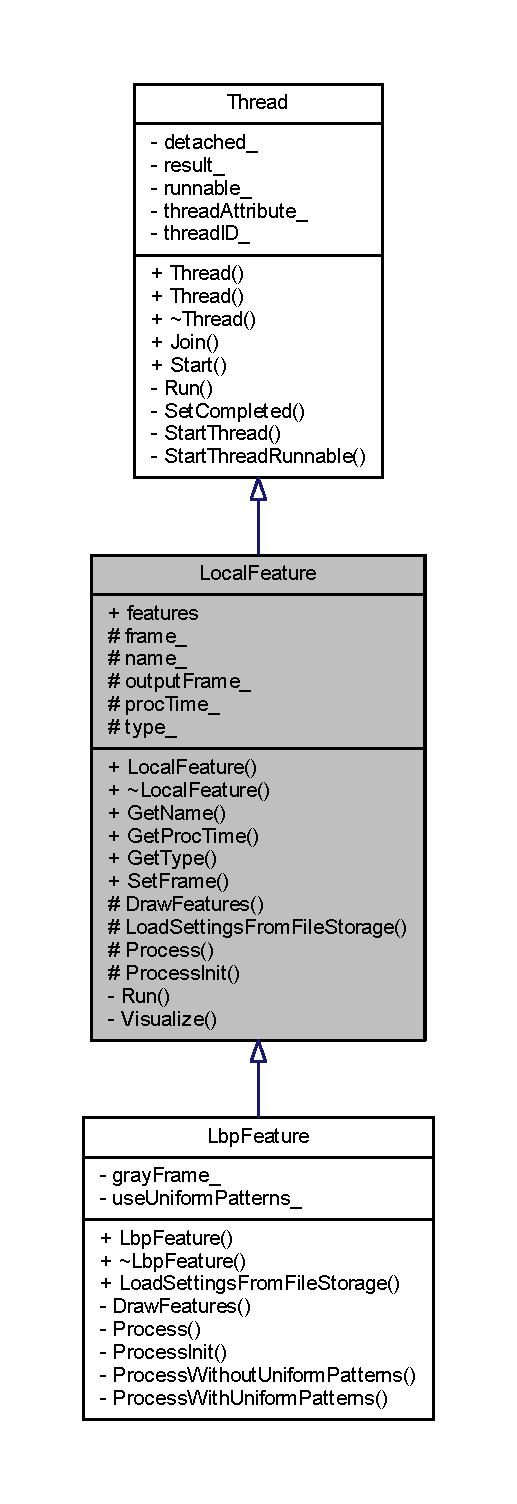
\includegraphics[height=550pt]{class_local_feature__inherit__graph}
\end{center}
\end{figure}


Collaboration diagram for Local\-Feature\-:
\nopagebreak
\begin{figure}[H]
\begin{center}
\leavevmode
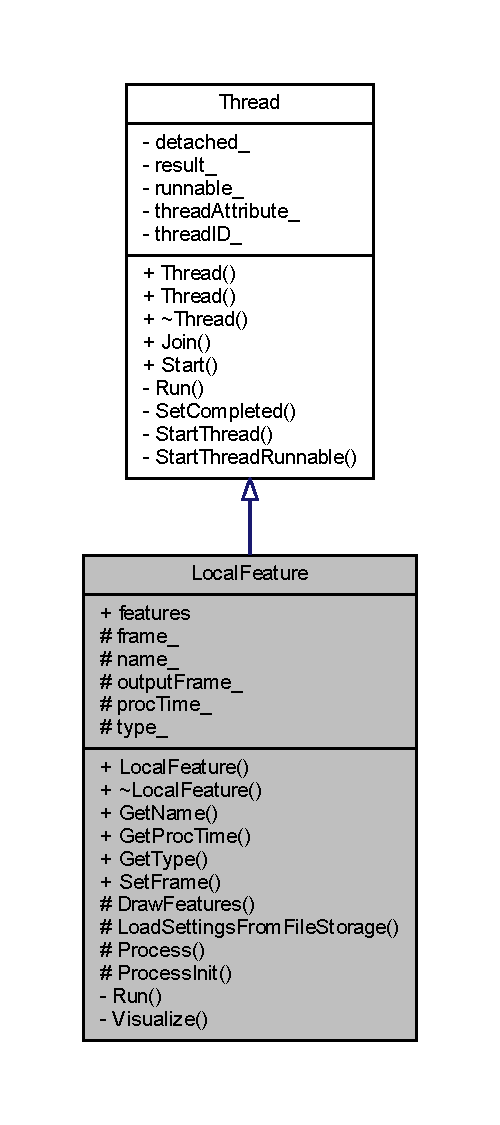
\includegraphics[width=240pt]{class_local_feature__coll__graph}
\end{center}
\end{figure}
\subsubsection*{Public Member Functions}
\begin{DoxyCompactItemize}
\item 
\hyperlink{group___feature_extractor_abc8f5b5d4088fd28be45cfd6b3d86cd5}{Local\-Feature} (const std\-::string \&name, const std\-::string \&type)
\begin{DoxyCompactList}\small\item\em Constructor. \end{DoxyCompactList}\item 
\hyperlink{group___feature_extractor_a457aceba33c8ef0f0ccaf4db8c679545}{$\sim$\-Local\-Feature} (void)
\begin{DoxyCompactList}\small\item\em Destructor. \end{DoxyCompactList}\item 
const std\-::string \& \hyperlink{group___feature_extractor_ab2ecc77360b2fa1400f29298a8e1b751}{Get\-Name} (void)
\begin{DoxyCompactList}\small\item\em Name getter. \end{DoxyCompactList}\item 
double \hyperlink{group___feature_extractor_a46f41fabf78e63d9e9c93cbaadf652a1}{Get\-Proc\-Time} (void)
\begin{DoxyCompactList}\small\item\em Process time getter. \end{DoxyCompactList}\item 
const std\-::string \& \hyperlink{group___feature_extractor_aba5fb3207f97ae73dc3cab7572baf85e}{Get\-Type} (void)
\begin{DoxyCompactList}\small\item\em Type getter. \end{DoxyCompactList}\item 
void $\ast$ \hyperlink{group___core_a8f33f7750321d5df9188033e7e3e300d}{Join} (void)
\item 
void \hyperlink{group___feature_extractor_aee5c4e09e373308e7f50bfaffd8e2267}{Set\-Frame} (const cv\-::\-Mat \&frame)
\begin{DoxyCompactList}\small\item\em Connects a frame to the feature extractor. \end{DoxyCompactList}\item 
void \hyperlink{group___core_a2b42f82341afd2747ea093b6ac8b91cb}{Start} (void)
\begin{DoxyCompactList}\small\item\em Starts the thread. \end{DoxyCompactList}\end{DoxyCompactItemize}
\subsubsection*{Public Attributes}
\begin{DoxyCompactItemize}
\item 
std\-::vector$<$ double $>$ \hyperlink{group___feature_extractor_a8197cec0d029bac380885167df9f65e5}{features}
\begin{DoxyCompactList}\small\item\em Stores local features. \end{DoxyCompactList}\end{DoxyCompactItemize}
\subsubsection*{Protected Member Functions}
\begin{DoxyCompactItemize}
\item 
virtual void \hyperlink{group___feature_extractor_a329c560d8f02a4ab390716319410deab}{Draw\-Features} (void)
\begin{DoxyCompactList}\small\item\em Virtual method for drawing the extracted features. \end{DoxyCompactList}\item 
virtual void \hyperlink{group___feature_extractor_a9280742c803d38c984121a33cdd67723}{Load\-Settings\-From\-File\-Storage} (void)
\begin{DoxyCompactList}\small\item\em Virtual method for loading algorithm specific settings from the given storage. \end{DoxyCompactList}\item 
virtual void \hyperlink{group___feature_extractor_a2f5b230fd63be9c1dcceb51361bc6ee1}{Process} (void)
\begin{DoxyCompactList}\small\item\em Virtual method for each feature extraction algorithm. \end{DoxyCompactList}\item 
virtual void \hyperlink{group___feature_extractor_a2b2cdc0b1be48785e967a87c268ee27e}{Process\-Init} (void)
\begin{DoxyCompactList}\small\item\em Virtual method for initalizing the variables. \end{DoxyCompactList}\end{DoxyCompactItemize}
\subsubsection*{Protected Attributes}
\begin{DoxyCompactItemize}
\item 
cv\-::\-Mat \hyperlink{group___feature_extractor_a585b0dc6e6184422c5563e80bff50ffa}{frame\-\_\-}
\begin{DoxyCompactList}\small\item\em The current frame. \end{DoxyCompactList}\item 
std\-::string \hyperlink{group___feature_extractor_a0e73ef0aed82c04f06b6eeb9a9b9be8b}{name\-\_\-}
\begin{DoxyCompactList}\small\item\em Name of the current feature extraction procedure. \end{DoxyCompactList}\item 
cv\-::\-Mat \hyperlink{group___feature_extractor_a1c7b8087feb05f02b09eb1b536d443e6}{output\-Frame\-\_\-}
\begin{DoxyCompactList}\small\item\em The current frame. \end{DoxyCompactList}\item 
double \hyperlink{group___feature_extractor_a79d60ce90ab8e6ccd66ff8f7da2365c7}{proc\-Time\-\_\-}
\begin{DoxyCompactList}\small\item\em Processing time of the current feature extraction method. \end{DoxyCompactList}\item 
std\-::string \hyperlink{group___feature_extractor_aaf3aef30088cd1be80e1770d0a9d945b}{type\-\_\-}
\begin{DoxyCompactList}\small\item\em Type of the current feature extraction procedure. \end{DoxyCompactList}\end{DoxyCompactItemize}
\subsubsection*{Private Member Functions}
\begin{DoxyCompactItemize}
\item 
void $\ast$ \hyperlink{group___feature_extractor_ad415c0f9a207eb30cedfb750d62731cf}{Run} (void)
\begin{DoxyCompactList}\small\item\em Implemented virtual method for the algorithm. \end{DoxyCompactList}\item 
void \hyperlink{group___feature_extractor_ab39886debe485d200a73b8c8d500544b}{Visualize} (void)
\begin{DoxyCompactList}\small\item\em Visualizing the output of feature extractor. \end{DoxyCompactList}\end{DoxyCompactItemize}


\paragraph{Constructor \& Destructor Documentation}
\hypertarget{group___feature_extractor_abc8f5b5d4088fd28be45cfd6b3d86cd5}{\index{Local\-Feature@{Local\-Feature}!Local\-Feature@{Local\-Feature}}
\index{Local\-Feature@{Local\-Feature}!LocalFeature@{Local\-Feature}}
\subparagraph[{Local\-Feature}]{\setlength{\rightskip}{0pt plus 5cm}Local\-Feature\-::\-Local\-Feature (
\begin{DoxyParamCaption}
\item[{const std\-::string \&}]{name, }
\item[{const std\-::string \&}]{type}
\end{DoxyParamCaption}
)}}\label{group___feature_extractor_abc8f5b5d4088fd28be45cfd6b3d86cd5}


Constructor. 

\begin{DoxyVerb}    \param name Name of the current feature extraction procedure.
\end{DoxyVerb}
 
\begin{DoxyParams}{Parameters}
{\em type} & Type of the current feature extraction procedure (global or local). \\
\hline
\end{DoxyParams}
\hypertarget{group___feature_extractor_a457aceba33c8ef0f0ccaf4db8c679545}{\index{Local\-Feature@{Local\-Feature}!$\sim$\-Local\-Feature@{$\sim$\-Local\-Feature}}
\index{$\sim$\-Local\-Feature@{$\sim$\-Local\-Feature}!LocalFeature@{Local\-Feature}}
\subparagraph[{$\sim$\-Local\-Feature}]{\setlength{\rightskip}{0pt plus 5cm}Local\-Feature\-::$\sim$\-Local\-Feature (
\begin{DoxyParamCaption}
\item[{void}]{}
\end{DoxyParamCaption}
)}}\label{group___feature_extractor_a457aceba33c8ef0f0ccaf4db8c679545}


Destructor. 



\paragraph{Member Function Documentation}
\hypertarget{group___feature_extractor_a329c560d8f02a4ab390716319410deab}{\index{Local\-Feature@{Local\-Feature}!Draw\-Features@{Draw\-Features}}
\index{Draw\-Features@{Draw\-Features}!LocalFeature@{Local\-Feature}}
\subparagraph[{Draw\-Features}]{\setlength{\rightskip}{0pt plus 5cm}virtual void Local\-Feature\-::\-Draw\-Features (
\begin{DoxyParamCaption}
\item[{void}]{}
\end{DoxyParamCaption}
)\hspace{0.3cm}{\ttfamily [protected]}, {\ttfamily [virtual]}}}\label{group___feature_extractor_a329c560d8f02a4ab390716319410deab}


Virtual method for drawing the extracted features. 



Reimplemented in \hyperlink{group___feature_extractor_a152c1785ca51eb7e5878c0d3f9309697}{Lbp\-Feature}.



Referenced by Run().



Here is the caller graph for this function\-:
\nopagebreak
\begin{figure}[H]
\begin{center}
\leavevmode
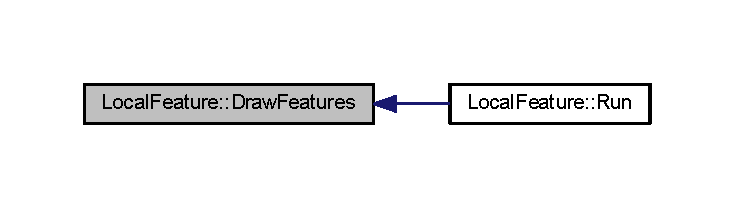
\includegraphics[width=350pt]{group___feature_extractor_a329c560d8f02a4ab390716319410deab_icgraph}
\end{center}
\end{figure}


\hypertarget{group___feature_extractor_ab2ecc77360b2fa1400f29298a8e1b751}{\index{Local\-Feature@{Local\-Feature}!Get\-Name@{Get\-Name}}
\index{Get\-Name@{Get\-Name}!LocalFeature@{Local\-Feature}}
\subparagraph[{Get\-Name}]{\setlength{\rightskip}{0pt plus 5cm}const string \& Local\-Feature\-::\-Get\-Name (
\begin{DoxyParamCaption}
\item[{void}]{}
\end{DoxyParamCaption}
)}}\label{group___feature_extractor_ab2ecc77360b2fa1400f29298a8e1b751}


Name getter. 

\begin{DoxyReturn}{Returns}
Name of the current feature extraction procedure. 
\end{DoxyReturn}


References name\-\_\-.

\hypertarget{group___feature_extractor_a46f41fabf78e63d9e9c93cbaadf652a1}{\index{Local\-Feature@{Local\-Feature}!Get\-Proc\-Time@{Get\-Proc\-Time}}
\index{Get\-Proc\-Time@{Get\-Proc\-Time}!LocalFeature@{Local\-Feature}}
\subparagraph[{Get\-Proc\-Time}]{\setlength{\rightskip}{0pt plus 5cm}double Local\-Feature\-::\-Get\-Proc\-Time (
\begin{DoxyParamCaption}
\item[{void}]{}
\end{DoxyParamCaption}
)}}\label{group___feature_extractor_a46f41fabf78e63d9e9c93cbaadf652a1}


Process time getter. 

\begin{DoxyReturn}{Returns}
Processing time of the current feature extraction method. 
\end{DoxyReturn}


References proc\-Time\-\_\-.

\hypertarget{group___feature_extractor_aba5fb3207f97ae73dc3cab7572baf85e}{\index{Local\-Feature@{Local\-Feature}!Get\-Type@{Get\-Type}}
\index{Get\-Type@{Get\-Type}!LocalFeature@{Local\-Feature}}
\subparagraph[{Get\-Type}]{\setlength{\rightskip}{0pt plus 5cm}const string \& Local\-Feature\-::\-Get\-Type (
\begin{DoxyParamCaption}
\item[{void}]{}
\end{DoxyParamCaption}
)}}\label{group___feature_extractor_aba5fb3207f97ae73dc3cab7572baf85e}


Type getter. 

\begin{DoxyReturn}{Returns}
Type of the current feature extraction procedure. 
\end{DoxyReturn}


References type\-\_\-.

\hypertarget{group___core_a8f33f7750321d5df9188033e7e3e300d}{\index{Local\-Feature@{Local\-Feature}!Join@{Join}}
\index{Join@{Join}!LocalFeature@{Local\-Feature}}
\subparagraph[{Join}]{\setlength{\rightskip}{0pt plus 5cm}void $\ast$ Thread\-::\-Join (
\begin{DoxyParamCaption}
\item[{void}]{}
\end{DoxyParamCaption}
)\hspace{0.3cm}{\ttfamily [inherited]}}}\label{group___core_a8f33f7750321d5df9188033e7e3e300d}


References Exception\-Error, Thread\-::result\-\_\-, and Thread\-::thread\-I\-D\-\_\-.

\hypertarget{group___feature_extractor_a9280742c803d38c984121a33cdd67723}{\index{Local\-Feature@{Local\-Feature}!Load\-Settings\-From\-File\-Storage@{Load\-Settings\-From\-File\-Storage}}
\index{Load\-Settings\-From\-File\-Storage@{Load\-Settings\-From\-File\-Storage}!LocalFeature@{Local\-Feature}}
\subparagraph[{Load\-Settings\-From\-File\-Storage}]{\setlength{\rightskip}{0pt plus 5cm}virtual void Local\-Feature\-::\-Load\-Settings\-From\-File\-Storage (
\begin{DoxyParamCaption}
\item[{void}]{}
\end{DoxyParamCaption}
)\hspace{0.3cm}{\ttfamily [protected]}, {\ttfamily [virtual]}}}\label{group___feature_extractor_a9280742c803d38c984121a33cdd67723}


Virtual method for loading algorithm specific settings from the given storage. 



Reimplemented in \hyperlink{group___feature_extractor_a39ac99c8b8537ac9d104ae4368177071}{Lbp\-Feature}.

\hypertarget{group___feature_extractor_a2f5b230fd63be9c1dcceb51361bc6ee1}{\index{Local\-Feature@{Local\-Feature}!Process@{Process}}
\index{Process@{Process}!LocalFeature@{Local\-Feature}}
\subparagraph[{Process}]{\setlength{\rightskip}{0pt plus 5cm}virtual void Local\-Feature\-::\-Process (
\begin{DoxyParamCaption}
\item[{void}]{}
\end{DoxyParamCaption}
)\hspace{0.3cm}{\ttfamily [protected]}, {\ttfamily [virtual]}}}\label{group___feature_extractor_a2f5b230fd63be9c1dcceb51361bc6ee1}


Virtual method for each feature extraction algorithm. 



Reimplemented in \hyperlink{group___feature_extractor_af664c189044d32f2cb71b334deb6f0c7}{Lbp\-Feature}.



Referenced by Run().



Here is the caller graph for this function\-:
\nopagebreak
\begin{figure}[H]
\begin{center}
\leavevmode
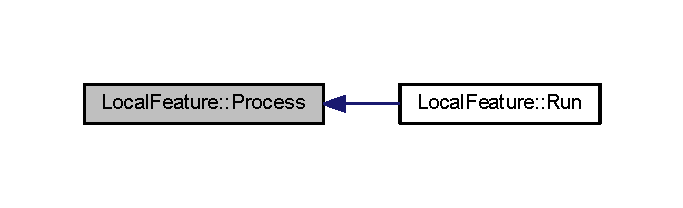
\includegraphics[width=328pt]{group___feature_extractor_a2f5b230fd63be9c1dcceb51361bc6ee1_icgraph}
\end{center}
\end{figure}


\hypertarget{group___feature_extractor_a2b2cdc0b1be48785e967a87c268ee27e}{\index{Local\-Feature@{Local\-Feature}!Process\-Init@{Process\-Init}}
\index{Process\-Init@{Process\-Init}!LocalFeature@{Local\-Feature}}
\subparagraph[{Process\-Init}]{\setlength{\rightskip}{0pt plus 5cm}virtual void Local\-Feature\-::\-Process\-Init (
\begin{DoxyParamCaption}
\item[{void}]{}
\end{DoxyParamCaption}
)\hspace{0.3cm}{\ttfamily [protected]}, {\ttfamily [virtual]}}}\label{group___feature_extractor_a2b2cdc0b1be48785e967a87c268ee27e}


Virtual method for initalizing the variables. 



Reimplemented in \hyperlink{group___feature_extractor_a773b1c3fd663f58b01f1ba33a897744f}{Lbp\-Feature}.



Referenced by Run().



Here is the caller graph for this function\-:
\nopagebreak
\begin{figure}[H]
\begin{center}
\leavevmode
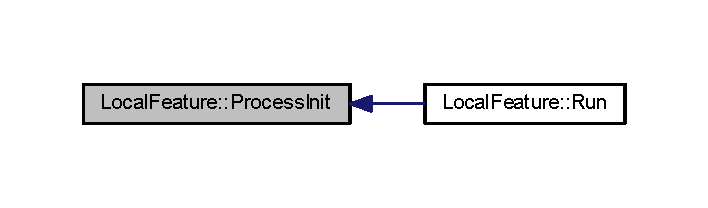
\includegraphics[width=340pt]{group___feature_extractor_a2b2cdc0b1be48785e967a87c268ee27e_icgraph}
\end{center}
\end{figure}


\hypertarget{group___feature_extractor_ad415c0f9a207eb30cedfb750d62731cf}{\index{Local\-Feature@{Local\-Feature}!Run@{Run}}
\index{Run@{Run}!LocalFeature@{Local\-Feature}}
\subparagraph[{Run}]{\setlength{\rightskip}{0pt plus 5cm}void $\ast$ Local\-Feature\-::\-Run (
\begin{DoxyParamCaption}
\item[{void}]{}
\end{DoxyParamCaption}
)\hspace{0.3cm}{\ttfamily [private]}, {\ttfamily [virtual]}}}\label{group___feature_extractor_ad415c0f9a207eb30cedfb750d62731cf}


Implemented virtual method for the algorithm. 

\begin{DoxySeeAlso}{See Also}
\hyperlink{group___core_ae46cda1b57e998b239a8b9710b0712e2}{Thread\-::\-Run()} 
\end{DoxySeeAlso}


Implements \hyperlink{group___core_ae46cda1b57e998b239a8b9710b0712e2}{Thread}.



References Draw\-Features(), frame\-\_\-, Process(), Process\-Init(), proc\-Time\-\_\-, and Visualize().



Here is the call graph for this function\-:
\nopagebreak
\begin{figure}[H]
\begin{center}
\leavevmode
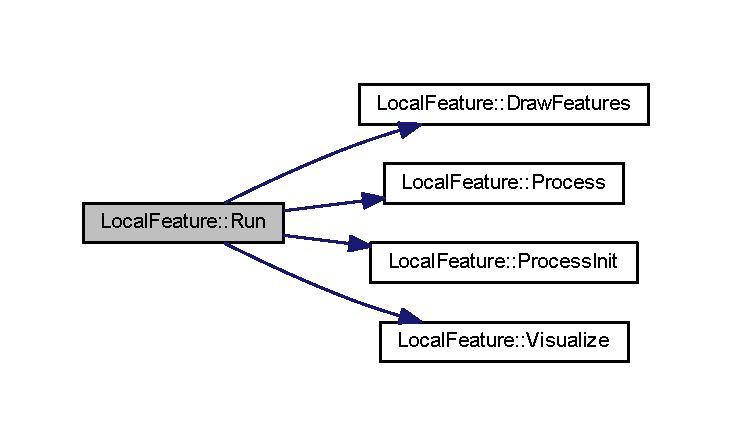
\includegraphics[width=350pt]{group___feature_extractor_ad415c0f9a207eb30cedfb750d62731cf_cgraph}
\end{center}
\end{figure}


\hypertarget{group___feature_extractor_aee5c4e09e373308e7f50bfaffd8e2267}{\index{Local\-Feature@{Local\-Feature}!Set\-Frame@{Set\-Frame}}
\index{Set\-Frame@{Set\-Frame}!LocalFeature@{Local\-Feature}}
\subparagraph[{Set\-Frame}]{\setlength{\rightskip}{0pt plus 5cm}void Local\-Feature\-::\-Set\-Frame (
\begin{DoxyParamCaption}
\item[{const cv\-::\-Mat \&}]{frame}
\end{DoxyParamCaption}
)}}\label{group___feature_extractor_aee5c4e09e373308e7f50bfaffd8e2267}


Connects a frame to the feature extractor. 


\begin{DoxyParams}{Parameters}
{\em frame} & Output parameter for the current frame. \\
\hline
\end{DoxyParams}


References frame\-\_\-.

\hypertarget{group___core_a2b42f82341afd2747ea093b6ac8b91cb}{\index{Local\-Feature@{Local\-Feature}!Start@{Start}}
\index{Start@{Start}!LocalFeature@{Local\-Feature}}
\subparagraph[{Start}]{\setlength{\rightskip}{0pt plus 5cm}void Thread\-::\-Start (
\begin{DoxyParamCaption}
\item[{void}]{}
\end{DoxyParamCaption}
)\hspace{0.3cm}{\ttfamily [inherited]}}}\label{group___core_a2b42f82341afd2747ea093b6ac8b91cb}


Starts the thread. 



References Thread\-::detached\-\_\-, Exception\-Error, Thread\-::runnable\-\_\-, Thread\-::\-Start\-Thread(), Thread\-::\-Start\-Thread\-Runnable(), Thread\-::thread\-Attribute\-\_\-, and Thread\-::thread\-I\-D\-\_\-.



Here is the call graph for this function\-:
\nopagebreak
\begin{figure}[H]
\begin{center}
\leavevmode
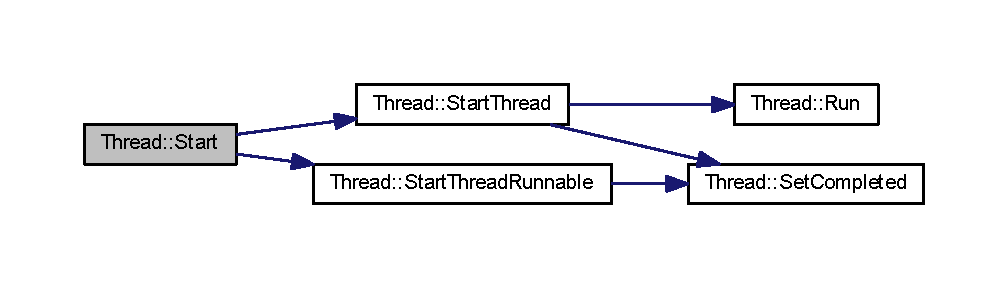
\includegraphics[width=350pt]{group___core_a2b42f82341afd2747ea093b6ac8b91cb_cgraph}
\end{center}
\end{figure}


\hypertarget{group___feature_extractor_ab39886debe485d200a73b8c8d500544b}{\index{Local\-Feature@{Local\-Feature}!Visualize@{Visualize}}
\index{Visualize@{Visualize}!LocalFeature@{Local\-Feature}}
\subparagraph[{Visualize}]{\setlength{\rightskip}{0pt plus 5cm}void Local\-Feature\-::\-Visualize (
\begin{DoxyParamCaption}
\item[{void}]{}
\end{DoxyParamCaption}
)\hspace{0.3cm}{\ttfamily [private]}}}\label{group___feature_extractor_ab39886debe485d200a73b8c8d500544b}


Visualizing the output of feature extractor. 


\begin{DoxyParams}{Parameters}
{\em key\-Points\-Count} & Number of the detected keypoints. \\
\hline
\end{DoxyParams}


References features, name\-\_\-, output\-Frame\-\_\-, proc\-Time\-\_\-, and Visualizer\-Ptr.



Referenced by Run().



Here is the caller graph for this function\-:
\nopagebreak
\begin{figure}[H]
\begin{center}
\leavevmode
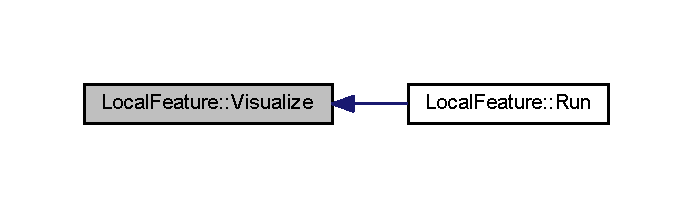
\includegraphics[width=332pt]{group___feature_extractor_ab39886debe485d200a73b8c8d500544b_icgraph}
\end{center}
\end{figure}




\paragraph{Member Data Documentation}
\hypertarget{group___feature_extractor_a8197cec0d029bac380885167df9f65e5}{\index{Local\-Feature@{Local\-Feature}!features@{features}}
\index{features@{features}!LocalFeature@{Local\-Feature}}
\subparagraph[{features}]{\setlength{\rightskip}{0pt plus 5cm}std\-::vector$<$double$>$ Local\-Feature\-::features}}\label{group___feature_extractor_a8197cec0d029bac380885167df9f65e5}


Stores local features. 



Referenced by Lbp\-Feature\-::\-Process(), Lbp\-Feature\-::\-Process\-Without\-Uniform\-Patterns(), Lbp\-Feature\-::\-Process\-With\-Uniform\-Patterns(), and Visualize().

\hypertarget{group___feature_extractor_a585b0dc6e6184422c5563e80bff50ffa}{\index{Local\-Feature@{Local\-Feature}!frame\-\_\-@{frame\-\_\-}}
\index{frame\-\_\-@{frame\-\_\-}!LocalFeature@{Local\-Feature}}
\subparagraph[{frame\-\_\-}]{\setlength{\rightskip}{0pt plus 5cm}cv\-::\-Mat Local\-Feature\-::frame\-\_\-\hspace{0.3cm}{\ttfamily [protected]}}}\label{group___feature_extractor_a585b0dc6e6184422c5563e80bff50ffa}


The current frame. 



Referenced by Lbp\-Feature\-::\-Process(), Lbp\-Feature\-::\-Process\-Init(), Lbp\-Feature\-::\-Process\-Without\-Uniform\-Patterns(), Lbp\-Feature\-::\-Process\-With\-Uniform\-Patterns(), Run(), and Set\-Frame().

\hypertarget{group___feature_extractor_a0e73ef0aed82c04f06b6eeb9a9b9be8b}{\index{Local\-Feature@{Local\-Feature}!name\-\_\-@{name\-\_\-}}
\index{name\-\_\-@{name\-\_\-}!LocalFeature@{Local\-Feature}}
\subparagraph[{name\-\_\-}]{\setlength{\rightskip}{0pt plus 5cm}std\-::string Local\-Feature\-::name\-\_\-\hspace{0.3cm}{\ttfamily [protected]}}}\label{group___feature_extractor_a0e73ef0aed82c04f06b6eeb9a9b9be8b}


Name of the current feature extraction procedure. 



Referenced by Get\-Name(), Lbp\-Feature\-::\-Load\-Settings\-From\-File\-Storage(), and Visualize().

\hypertarget{group___feature_extractor_a1c7b8087feb05f02b09eb1b536d443e6}{\index{Local\-Feature@{Local\-Feature}!output\-Frame\-\_\-@{output\-Frame\-\_\-}}
\index{output\-Frame\-\_\-@{output\-Frame\-\_\-}!LocalFeature@{Local\-Feature}}
\subparagraph[{output\-Frame\-\_\-}]{\setlength{\rightskip}{0pt plus 5cm}cv\-::\-Mat Local\-Feature\-::output\-Frame\-\_\-\hspace{0.3cm}{\ttfamily [protected]}}}\label{group___feature_extractor_a1c7b8087feb05f02b09eb1b536d443e6}


The current frame. 



Referenced by Lbp\-Feature\-::\-Process\-Init(), Lbp\-Feature\-::\-Process\-Without\-Uniform\-Patterns(), Lbp\-Feature\-::\-Process\-With\-Uniform\-Patterns(), and Visualize().

\hypertarget{group___feature_extractor_a79d60ce90ab8e6ccd66ff8f7da2365c7}{\index{Local\-Feature@{Local\-Feature}!proc\-Time\-\_\-@{proc\-Time\-\_\-}}
\index{proc\-Time\-\_\-@{proc\-Time\-\_\-}!LocalFeature@{Local\-Feature}}
\subparagraph[{proc\-Time\-\_\-}]{\setlength{\rightskip}{0pt plus 5cm}double Local\-Feature\-::proc\-Time\-\_\-\hspace{0.3cm}{\ttfamily [protected]}}}\label{group___feature_extractor_a79d60ce90ab8e6ccd66ff8f7da2365c7}


Processing time of the current feature extraction method. 



Referenced by Get\-Proc\-Time(), Run(), and Visualize().

\hypertarget{group___feature_extractor_aaf3aef30088cd1be80e1770d0a9d945b}{\index{Local\-Feature@{Local\-Feature}!type\-\_\-@{type\-\_\-}}
\index{type\-\_\-@{type\-\_\-}!LocalFeature@{Local\-Feature}}
\subparagraph[{type\-\_\-}]{\setlength{\rightskip}{0pt plus 5cm}std\-::string Local\-Feature\-::type\-\_\-\hspace{0.3cm}{\ttfamily [protected]}}}\label{group___feature_extractor_aaf3aef30088cd1be80e1770d0a9d945b}


Type of the current feature extraction procedure. 



Referenced by Get\-Type().

\index{Mser\-Feature@{Mser\-Feature}}\label{class_mser_feature}
\hypertarget{group___feature_extractor_class_mser_feature}{}
\subsubsection{class Mser\-Feature}
Class for extracting M\-S\-E\-R features. 

\begin{DoxyVerb}The class implements Maximally-Stable Extremal Region Extractor algorithm.
\end{DoxyVerb}
 The class encapsulates all the parameters of M\-S\-E\-R (see \href{http://en.wikipedia.org/wiki/Maximally_stable_extremal_regions}{\tt http\-://en.\-wikipedia.\-org/wiki/\-Maximally\-\_\-stable\-\_\-extremal\-\_\-regions} ) extraction algorithm. 

Inheritance diagram for Mser\-Feature\-:
\nopagebreak
\begin{figure}[H]
\begin{center}
\leavevmode
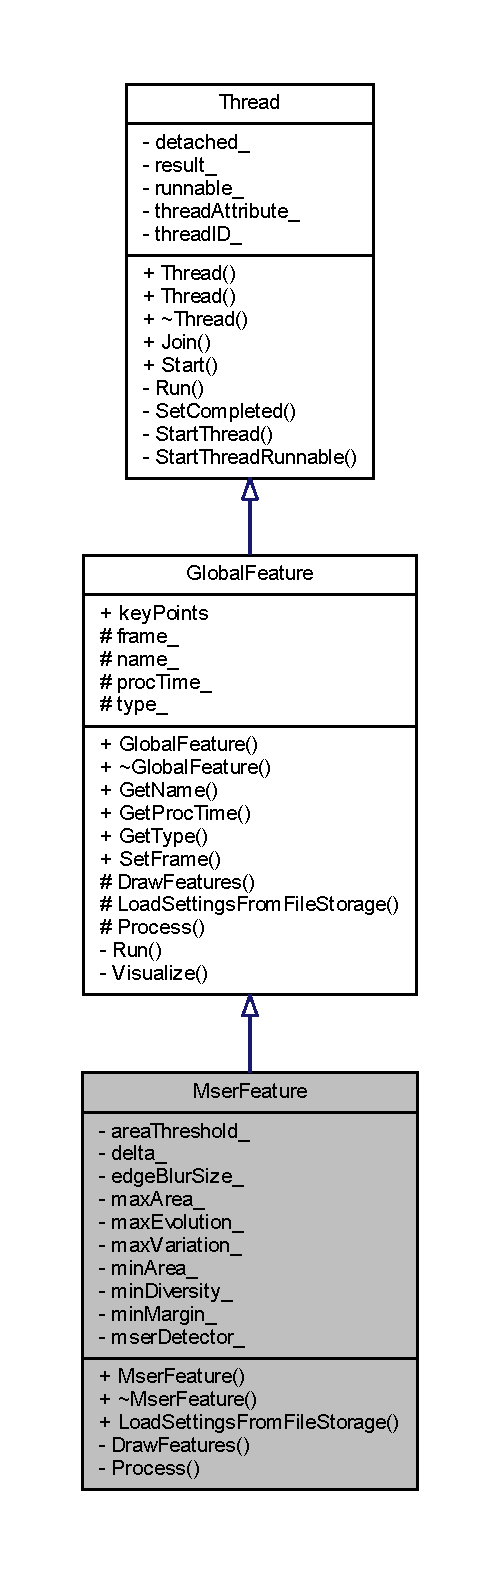
\includegraphics[height=550pt]{class_mser_feature__inherit__graph}
\end{center}
\end{figure}


Collaboration diagram for Mser\-Feature\-:
\nopagebreak
\begin{figure}[H]
\begin{center}
\leavevmode
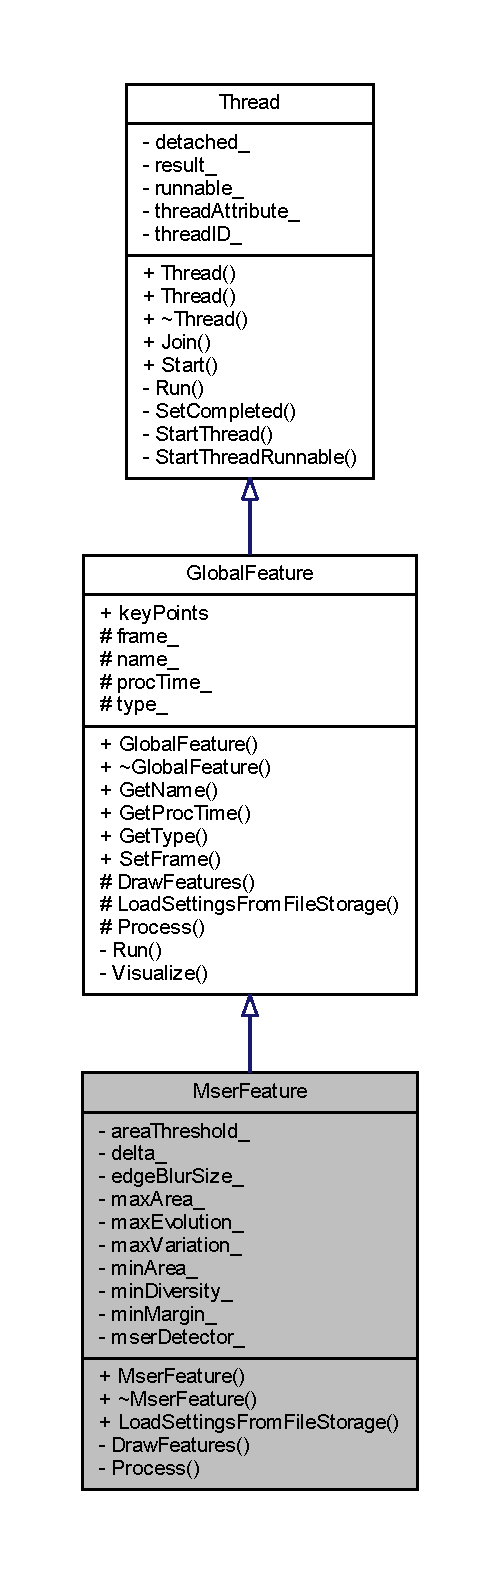
\includegraphics[height=550pt]{class_mser_feature__coll__graph}
\end{center}
\end{figure}
\subsubsection*{Public Member Functions}
\begin{DoxyCompactItemize}
\item 
\hyperlink{group___feature_extractor_ae82ba666f45d0f4d88be995ae5b6209c}{Mser\-Feature} (const std\-::string \&name, const std\-::string \&type)
\begin{DoxyCompactList}\small\item\em Constructor. \end{DoxyCompactList}\item 
\hyperlink{group___feature_extractor_a4cf98957c8813b3ec26641ded124340d}{$\sim$\-Mser\-Feature} (void)
\begin{DoxyCompactList}\small\item\em Destructor. \end{DoxyCompactList}\item 
const std\-::string \& \hyperlink{group___feature_extractor_a5f69ca2455d5eec4493dbf115d00d5c9}{Get\-Name} (void)
\begin{DoxyCompactList}\small\item\em Name getter. \end{DoxyCompactList}\item 
double \hyperlink{group___feature_extractor_ad07a3104192b50d911eee634a0be009d}{Get\-Proc\-Time} (void)
\begin{DoxyCompactList}\small\item\em Process time getter. \end{DoxyCompactList}\item 
const std\-::string \& \hyperlink{group___feature_extractor_a6724c19006d495bd6a9c8c6029236ebc}{Get\-Type} (void)
\begin{DoxyCompactList}\small\item\em Type getter. \end{DoxyCompactList}\item 
void $\ast$ \hyperlink{group___core_a8f33f7750321d5df9188033e7e3e300d}{Join} (void)
\item 
void \hyperlink{group___feature_extractor_ae6c9bca2395a33ecac78a46e9c331979}{Load\-Settings\-From\-File\-Storage} (void)
\begin{DoxyCompactList}\small\item\em Implemented virtual method for loading algorithm specific settings from the given storage. \end{DoxyCompactList}\item 
void \hyperlink{group___feature_extractor_a3c58d995fb2440b28db3b21b54b94815}{Set\-Frame} (const cv\-::\-Mat \&frame)
\begin{DoxyCompactList}\small\item\em Connects a frame to the feature extractor. \end{DoxyCompactList}\item 
void \hyperlink{group___core_a2b42f82341afd2747ea093b6ac8b91cb}{Start} (void)
\begin{DoxyCompactList}\small\item\em Starts the thread. \end{DoxyCompactList}\end{DoxyCompactItemize}
\subsubsection*{Public Attributes}
\begin{DoxyCompactItemize}
\item 
std\-::vector$<$ cv\-::\-Key\-Point $>$ \hyperlink{group___feature_extractor_a72cc606c0090a64718a7e92bca7520b9}{key\-Points}
\begin{DoxyCompactList}\small\item\em Stores keypoints, i.\-e. a point feature found by one of many available keypoint detectors. \end{DoxyCompactList}\end{DoxyCompactItemize}
\subsubsection*{Protected Attributes}
\begin{DoxyCompactItemize}
\item 
cv\-::\-Mat \hyperlink{group___feature_extractor_aae4295da2c3999edcb99b46d70ee7166}{frame\-\_\-}
\begin{DoxyCompactList}\small\item\em The current frame. \end{DoxyCompactList}\item 
std\-::string \hyperlink{group___feature_extractor_abee52be830de272bd27685083bf28aae}{name\-\_\-}
\begin{DoxyCompactList}\small\item\em Name of the current feature extraction procedure. \end{DoxyCompactList}\item 
double \hyperlink{group___feature_extractor_aa3306975b929f5503dac51829f9e04a0}{proc\-Time\-\_\-}
\begin{DoxyCompactList}\small\item\em Processing time of the current feature extraction method. \end{DoxyCompactList}\item 
std\-::string \hyperlink{group___feature_extractor_ad467857c4bc3d0fe65ba29e3b8f7c796}{type\-\_\-}
\begin{DoxyCompactList}\small\item\em Type of the current feature extraction procedure. \end{DoxyCompactList}\end{DoxyCompactItemize}
\subsubsection*{Private Member Functions}
\begin{DoxyCompactItemize}
\item 
void \hyperlink{group___feature_extractor_abed40317b412e0046df5772367d4f3dc}{Draw\-Features} (void)
\begin{DoxyCompactList}\small\item\em Implemented virtual method for displaying the output. \end{DoxyCompactList}\item 
void \hyperlink{group___feature_extractor_ad96a1235b0c0df21e68c5a2742debacb}{Process} (void)
\begin{DoxyCompactList}\small\item\em Implemented virtual method for the algorithm. \end{DoxyCompactList}\end{DoxyCompactItemize}
\subsubsection*{Private Attributes}
\begin{DoxyCompactItemize}
\item 
double \hyperlink{group___feature_extractor_ade4ed6ec57dbfefd1a263fa29419e54d}{area\-Threshold\-\_\-}
\begin{DoxyCompactList}\small\item\em The area threshold to cause re-\/initialize. \end{DoxyCompactList}\item 
int \hyperlink{group___feature_extractor_a55dae2de52e614532d2243ca113fb3fb}{delta\-\_\-}
\begin{DoxyCompactList}\small\item\em Delta in the code, it compares (size\-\_\-\{i\} -\/ size\-\_\-\{i -\/ delta\}) / size\-\_\-\{i -\/ delta\}. \end{DoxyCompactList}\item 
int \hyperlink{group___feature_extractor_a1850b5af2915831475ef9d776e8a72ea}{edge\-Blur\-Size\-\_\-}
\begin{DoxyCompactList}\small\item\em The aperture size for edge blur. \end{DoxyCompactList}\item 
int \hyperlink{group___feature_extractor_a74d77b8596474323f1c4581ddf1d7fa2}{max\-Area\-\_\-}
\begin{DoxyCompactList}\small\item\em Prune the area which bigger than max\-Area. \end{DoxyCompactList}\item 
int \hyperlink{group___feature_extractor_a135d54a9a46522e800ef26ecfb8f18be}{max\-Evolution\-\_\-}
\begin{DoxyCompactList}\small\item\em For color image, the evolution steps. \end{DoxyCompactList}\item 
double \hyperlink{group___feature_extractor_a9353f0657019b0177c8ce65c00d826f4}{max\-Variation\-\_\-}
\begin{DoxyCompactList}\small\item\em Prune the area have simliar size to its children. \end{DoxyCompactList}\item 
int \hyperlink{group___feature_extractor_a556156bf90c6cff20f7451134dc5c9f3}{min\-Area\-\_\-}
\begin{DoxyCompactList}\small\item\em Prune the area which smaller than min\-Area. \end{DoxyCompactList}\item 
double \hyperlink{group___feature_extractor_a7f7fe51c62b96bcc83f51e73e0d59a94}{min\-Diversity\-\_\-}
\begin{DoxyCompactList}\small\item\em Trace back to cut off mser with diversity $<$ min\-\_\-diversity. \end{DoxyCompactList}\item 
double \hyperlink{group___feature_extractor_a6bc22c26631b87ff8787244da9d1eca2}{min\-Margin\-\_\-}
\begin{DoxyCompactList}\small\item\em Ignore too small margin. \end{DoxyCompactList}\item 
cv\-::\-Mser\-Feature\-Detector $\ast$ \hyperlink{group___feature_extractor_a4e7332139a72f3591cbc2e02e7f67748}{mser\-Detector\-\_\-}
\begin{DoxyCompactList}\small\item\em Wrapped Open\-C\-V M\-S\-E\-R object. \end{DoxyCompactList}\end{DoxyCompactItemize}


\paragraph{Constructor \& Destructor Documentation}
\hypertarget{group___feature_extractor_ae82ba666f45d0f4d88be995ae5b6209c}{\index{Mser\-Feature@{Mser\-Feature}!Mser\-Feature@{Mser\-Feature}}
\index{Mser\-Feature@{Mser\-Feature}!MserFeature@{Mser\-Feature}}
\subparagraph[{Mser\-Feature}]{\setlength{\rightskip}{0pt plus 5cm}Mser\-Feature\-::\-Mser\-Feature (
\begin{DoxyParamCaption}
\item[{const std\-::string \&}]{name, }
\item[{const std\-::string \&}]{type}
\end{DoxyParamCaption}
)}}\label{group___feature_extractor_ae82ba666f45d0f4d88be995ae5b6209c}


Constructor. 

\begin{DoxyVerb}    \param name Name of the current feature extraction procedure.
\end{DoxyVerb}
 
\begin{DoxyParams}{Parameters}
{\em type} & Type of the current feature extraction procedure (global or local). \\
\hline
\end{DoxyParams}


References area\-Threshold\-\_\-, delta\-\_\-, edge\-Blur\-Size\-\_\-, Load\-Settings\-From\-File\-Storage(), max\-Area\-\_\-, max\-Evolution\-\_\-, max\-Variation\-\_\-, min\-Area\-\_\-, min\-Diversity\-\_\-, min\-Margin\-\_\-, and mser\-Detector\-\_\-.



Here is the call graph for this function\-:
\nopagebreak
\begin{figure}[H]
\begin{center}
\leavevmode
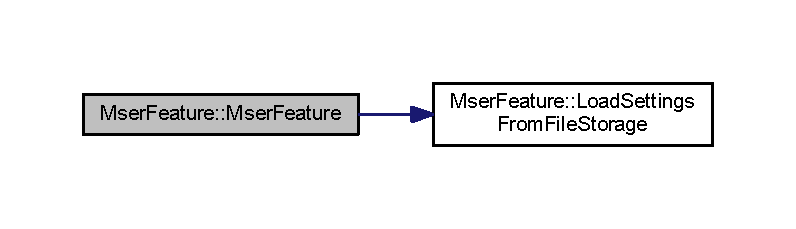
\includegraphics[width=350pt]{group___feature_extractor_ae82ba666f45d0f4d88be995ae5b6209c_cgraph}
\end{center}
\end{figure}


\hypertarget{group___feature_extractor_a4cf98957c8813b3ec26641ded124340d}{\index{Mser\-Feature@{Mser\-Feature}!$\sim$\-Mser\-Feature@{$\sim$\-Mser\-Feature}}
\index{$\sim$\-Mser\-Feature@{$\sim$\-Mser\-Feature}!MserFeature@{Mser\-Feature}}
\subparagraph[{$\sim$\-Mser\-Feature}]{\setlength{\rightskip}{0pt plus 5cm}Mser\-Feature\-::$\sim$\-Mser\-Feature (
\begin{DoxyParamCaption}
\item[{void}]{}
\end{DoxyParamCaption}
)}}\label{group___feature_extractor_a4cf98957c8813b3ec26641ded124340d}


Destructor. 



References mser\-Detector\-\_\-.



\paragraph{Member Function Documentation}
\hypertarget{group___feature_extractor_abed40317b412e0046df5772367d4f3dc}{\index{Mser\-Feature@{Mser\-Feature}!Draw\-Features@{Draw\-Features}}
\index{Draw\-Features@{Draw\-Features}!MserFeature@{Mser\-Feature}}
\subparagraph[{Draw\-Features}]{\setlength{\rightskip}{0pt plus 5cm}void Mser\-Feature\-::\-Draw\-Features (
\begin{DoxyParamCaption}
\item[{void}]{}
\end{DoxyParamCaption}
)\hspace{0.3cm}{\ttfamily [private]}, {\ttfamily [virtual]}}}\label{group___feature_extractor_abed40317b412e0046df5772367d4f3dc}


Implemented virtual method for displaying the output. 

\begin{DoxySeeAlso}{See Also}
\hyperlink{group___feature_extractor_acea1ee12c177894819ea7ae0f6294e5c}{Global\-Feature\-::\-Draw\-Features()} 
\end{DoxySeeAlso}


Reimplemented from \hyperlink{group___feature_extractor_acea1ee12c177894819ea7ae0f6294e5c}{Global\-Feature}.



References Global\-Feature\-::frame\-\_\-, and Global\-Feature\-::key\-Points.

\hypertarget{group___feature_extractor_a5f69ca2455d5eec4493dbf115d00d5c9}{\index{Mser\-Feature@{Mser\-Feature}!Get\-Name@{Get\-Name}}
\index{Get\-Name@{Get\-Name}!MserFeature@{Mser\-Feature}}
\subparagraph[{Get\-Name}]{\setlength{\rightskip}{0pt plus 5cm}const string \& Global\-Feature\-::\-Get\-Name (
\begin{DoxyParamCaption}
\item[{void}]{}
\end{DoxyParamCaption}
)\hspace{0.3cm}{\ttfamily [inherited]}}}\label{group___feature_extractor_a5f69ca2455d5eec4493dbf115d00d5c9}


Name getter. 

\begin{DoxyReturn}{Returns}
Name of the current feature extraction procedure. 
\end{DoxyReturn}


References Global\-Feature\-::name\-\_\-.

\hypertarget{group___feature_extractor_ad07a3104192b50d911eee634a0be009d}{\index{Mser\-Feature@{Mser\-Feature}!Get\-Proc\-Time@{Get\-Proc\-Time}}
\index{Get\-Proc\-Time@{Get\-Proc\-Time}!MserFeature@{Mser\-Feature}}
\subparagraph[{Get\-Proc\-Time}]{\setlength{\rightskip}{0pt plus 5cm}double Global\-Feature\-::\-Get\-Proc\-Time (
\begin{DoxyParamCaption}
\item[{void}]{}
\end{DoxyParamCaption}
)\hspace{0.3cm}{\ttfamily [inherited]}}}\label{group___feature_extractor_ad07a3104192b50d911eee634a0be009d}


Process time getter. 

\begin{DoxyReturn}{Returns}
Processing time of the current feature extraction method. 
\end{DoxyReturn}


References Global\-Feature\-::proc\-Time\-\_\-.

\hypertarget{group___feature_extractor_a6724c19006d495bd6a9c8c6029236ebc}{\index{Mser\-Feature@{Mser\-Feature}!Get\-Type@{Get\-Type}}
\index{Get\-Type@{Get\-Type}!MserFeature@{Mser\-Feature}}
\subparagraph[{Get\-Type}]{\setlength{\rightskip}{0pt plus 5cm}const string \& Global\-Feature\-::\-Get\-Type (
\begin{DoxyParamCaption}
\item[{void}]{}
\end{DoxyParamCaption}
)\hspace{0.3cm}{\ttfamily [inherited]}}}\label{group___feature_extractor_a6724c19006d495bd6a9c8c6029236ebc}


Type getter. 

\begin{DoxyReturn}{Returns}
Type of the current feature extraction procedure. 
\end{DoxyReturn}


References Global\-Feature\-::type\-\_\-.

\hypertarget{group___core_a8f33f7750321d5df9188033e7e3e300d}{\index{Mser\-Feature@{Mser\-Feature}!Join@{Join}}
\index{Join@{Join}!MserFeature@{Mser\-Feature}}
\subparagraph[{Join}]{\setlength{\rightskip}{0pt plus 5cm}void $\ast$ Thread\-::\-Join (
\begin{DoxyParamCaption}
\item[{void}]{}
\end{DoxyParamCaption}
)\hspace{0.3cm}{\ttfamily [inherited]}}}\label{group___core_a8f33f7750321d5df9188033e7e3e300d}


References Exception\-Error, Thread\-::result\-\_\-, and Thread\-::thread\-I\-D\-\_\-.

\hypertarget{group___feature_extractor_ae6c9bca2395a33ecac78a46e9c331979}{\index{Mser\-Feature@{Mser\-Feature}!Load\-Settings\-From\-File\-Storage@{Load\-Settings\-From\-File\-Storage}}
\index{Load\-Settings\-From\-File\-Storage@{Load\-Settings\-From\-File\-Storage}!MserFeature@{Mser\-Feature}}
\subparagraph[{Load\-Settings\-From\-File\-Storage}]{\setlength{\rightskip}{0pt plus 5cm}void Mser\-Feature\-::\-Load\-Settings\-From\-File\-Storage (
\begin{DoxyParamCaption}
\item[{void}]{}
\end{DoxyParamCaption}
)\hspace{0.3cm}{\ttfamily [virtual]}}}\label{group___feature_extractor_ae6c9bca2395a33ecac78a46e9c331979}


Implemented virtual method for loading algorithm specific settings from the given storage. 

\begin{DoxySeeAlso}{See Also}
\hyperlink{group___feature_extractor_aa48133762d9f52a5c2ae5042f6ebbe71}{Global\-Feature\-::\-Load\-Settings\-From\-File\-Storage()} 
\end{DoxySeeAlso}


Reimplemented from \hyperlink{group___feature_extractor_aa48133762d9f52a5c2ae5042f6ebbe71}{Global\-Feature}.



References area\-Threshold\-\_\-, delta\-\_\-, edge\-Blur\-Size\-\_\-, Exception\-Error, Local\-Settings\-Ptr, max\-Area\-\_\-, max\-Evolution\-\_\-, max\-Variation\-\_\-, min\-Area\-\_\-, min\-Diversity\-\_\-, min\-Margin\-\_\-, and Global\-Feature\-::name\-\_\-.



Referenced by Mser\-Feature().



Here is the caller graph for this function\-:
\nopagebreak
\begin{figure}[H]
\begin{center}
\leavevmode
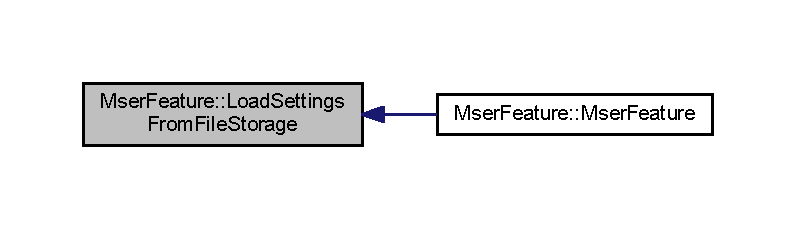
\includegraphics[width=350pt]{group___feature_extractor_ae6c9bca2395a33ecac78a46e9c331979_icgraph}
\end{center}
\end{figure}


\hypertarget{group___feature_extractor_ad96a1235b0c0df21e68c5a2742debacb}{\index{Mser\-Feature@{Mser\-Feature}!Process@{Process}}
\index{Process@{Process}!MserFeature@{Mser\-Feature}}
\subparagraph[{Process}]{\setlength{\rightskip}{0pt plus 5cm}void Mser\-Feature\-::\-Process (
\begin{DoxyParamCaption}
\item[{void}]{}
\end{DoxyParamCaption}
)\hspace{0.3cm}{\ttfamily [private]}, {\ttfamily [virtual]}}}\label{group___feature_extractor_ad96a1235b0c0df21e68c5a2742debacb}


Implemented virtual method for the algorithm. 

\begin{DoxySeeAlso}{See Also}
\hyperlink{group___feature_extractor_a9fdfc934c5a9da6962ec39c1b0cf32dc}{Global\-Feature\-::\-Process()} 
\end{DoxySeeAlso}


Reimplemented from \hyperlink{group___feature_extractor_a9fdfc934c5a9da6962ec39c1b0cf32dc}{Global\-Feature}.



References Global\-Feature\-::frame\-\_\-, Global\-Feature\-::key\-Points, and mser\-Detector\-\_\-.

\hypertarget{group___feature_extractor_a3c58d995fb2440b28db3b21b54b94815}{\index{Mser\-Feature@{Mser\-Feature}!Set\-Frame@{Set\-Frame}}
\index{Set\-Frame@{Set\-Frame}!MserFeature@{Mser\-Feature}}
\subparagraph[{Set\-Frame}]{\setlength{\rightskip}{0pt plus 5cm}void Global\-Feature\-::\-Set\-Frame (
\begin{DoxyParamCaption}
\item[{const cv\-::\-Mat \&}]{frame}
\end{DoxyParamCaption}
)\hspace{0.3cm}{\ttfamily [inherited]}}}\label{group___feature_extractor_a3c58d995fb2440b28db3b21b54b94815}


Connects a frame to the feature extractor. 


\begin{DoxyParams}{Parameters}
{\em frame} & Output parameter for the current frame. \\
\hline
\end{DoxyParams}


References Global\-Feature\-::frame\-\_\-.

\hypertarget{group___core_a2b42f82341afd2747ea093b6ac8b91cb}{\index{Mser\-Feature@{Mser\-Feature}!Start@{Start}}
\index{Start@{Start}!MserFeature@{Mser\-Feature}}
\subparagraph[{Start}]{\setlength{\rightskip}{0pt plus 5cm}void Thread\-::\-Start (
\begin{DoxyParamCaption}
\item[{void}]{}
\end{DoxyParamCaption}
)\hspace{0.3cm}{\ttfamily [inherited]}}}\label{group___core_a2b42f82341afd2747ea093b6ac8b91cb}


Starts the thread. 



References Thread\-::detached\-\_\-, Exception\-Error, Thread\-::runnable\-\_\-, Thread\-::\-Start\-Thread(), Thread\-::\-Start\-Thread\-Runnable(), Thread\-::thread\-Attribute\-\_\-, and Thread\-::thread\-I\-D\-\_\-.



Here is the call graph for this function\-:
\nopagebreak
\begin{figure}[H]
\begin{center}
\leavevmode
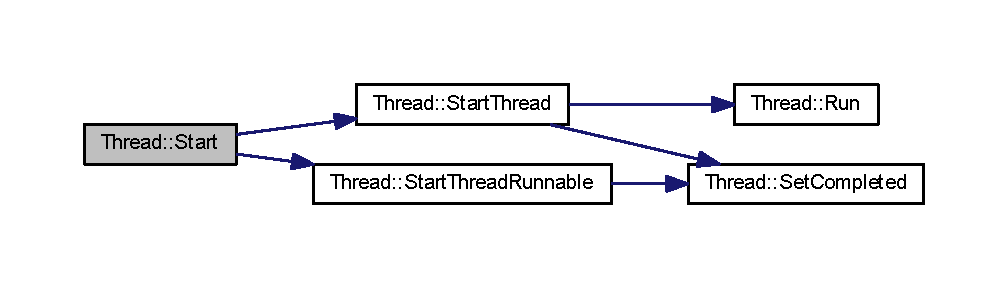
\includegraphics[width=350pt]{group___core_a2b42f82341afd2747ea093b6ac8b91cb_cgraph}
\end{center}
\end{figure}




\paragraph{Member Data Documentation}
\hypertarget{group___feature_extractor_ade4ed6ec57dbfefd1a263fa29419e54d}{\index{Mser\-Feature@{Mser\-Feature}!area\-Threshold\-\_\-@{area\-Threshold\-\_\-}}
\index{area\-Threshold\-\_\-@{area\-Threshold\-\_\-}!MserFeature@{Mser\-Feature}}
\subparagraph[{area\-Threshold\-\_\-}]{\setlength{\rightskip}{0pt plus 5cm}double Mser\-Feature\-::area\-Threshold\-\_\-\hspace{0.3cm}{\ttfamily [private]}}}\label{group___feature_extractor_ade4ed6ec57dbfefd1a263fa29419e54d}


The area threshold to cause re-\/initialize. 



Referenced by Load\-Settings\-From\-File\-Storage(), and Mser\-Feature().

\hypertarget{group___feature_extractor_a55dae2de52e614532d2243ca113fb3fb}{\index{Mser\-Feature@{Mser\-Feature}!delta\-\_\-@{delta\-\_\-}}
\index{delta\-\_\-@{delta\-\_\-}!MserFeature@{Mser\-Feature}}
\subparagraph[{delta\-\_\-}]{\setlength{\rightskip}{0pt plus 5cm}int Mser\-Feature\-::delta\-\_\-\hspace{0.3cm}{\ttfamily [private]}}}\label{group___feature_extractor_a55dae2de52e614532d2243ca113fb3fb}


Delta in the code, it compares (size\-\_\-\{i\} -\/ size\-\_\-\{i -\/ delta\}) / size\-\_\-\{i -\/ delta\}. 



Referenced by Load\-Settings\-From\-File\-Storage(), and Mser\-Feature().

\hypertarget{group___feature_extractor_a1850b5af2915831475ef9d776e8a72ea}{\index{Mser\-Feature@{Mser\-Feature}!edge\-Blur\-Size\-\_\-@{edge\-Blur\-Size\-\_\-}}
\index{edge\-Blur\-Size\-\_\-@{edge\-Blur\-Size\-\_\-}!MserFeature@{Mser\-Feature}}
\subparagraph[{edge\-Blur\-Size\-\_\-}]{\setlength{\rightskip}{0pt plus 5cm}int Mser\-Feature\-::edge\-Blur\-Size\-\_\-\hspace{0.3cm}{\ttfamily [private]}}}\label{group___feature_extractor_a1850b5af2915831475ef9d776e8a72ea}


The aperture size for edge blur. 



Referenced by Load\-Settings\-From\-File\-Storage(), and Mser\-Feature().

\hypertarget{group___feature_extractor_aae4295da2c3999edcb99b46d70ee7166}{\index{Mser\-Feature@{Mser\-Feature}!frame\-\_\-@{frame\-\_\-}}
\index{frame\-\_\-@{frame\-\_\-}!MserFeature@{Mser\-Feature}}
\subparagraph[{frame\-\_\-}]{\setlength{\rightskip}{0pt plus 5cm}cv\-::\-Mat Global\-Feature\-::frame\-\_\-\hspace{0.3cm}{\ttfamily [protected]}, {\ttfamily [inherited]}}}\label{group___feature_extractor_aae4295da2c3999edcb99b46d70ee7166}


The current frame. 



Referenced by Draw\-Features(), Star\-Feature\-::\-Draw\-Features(), Fast\-Feature\-::\-Draw\-Features(), Orb\-Feature\-::\-Draw\-Features(), Sift\-Feature\-::\-Draw\-Features(), Surf\-Feature\-::\-Draw\-Features(), Star\-Feature\-::\-Process(), Process(), Fast\-Feature\-::\-Process(), Orb\-Feature\-::\-Process(), Surf\-Feature\-::\-Process(), Sift\-Feature\-::\-Process(), Global\-Feature\-::\-Run(), Global\-Feature\-::\-Set\-Frame(), and Global\-Feature\-::\-Visualize().

\hypertarget{group___feature_extractor_a72cc606c0090a64718a7e92bca7520b9}{\index{Mser\-Feature@{Mser\-Feature}!key\-Points@{key\-Points}}
\index{key\-Points@{key\-Points}!MserFeature@{Mser\-Feature}}
\subparagraph[{key\-Points}]{\setlength{\rightskip}{0pt plus 5cm}std\-::vector$<$cv\-::\-Key\-Point$>$ Global\-Feature\-::key\-Points\hspace{0.3cm}{\ttfamily [inherited]}}}\label{group___feature_extractor_a72cc606c0090a64718a7e92bca7520b9}


Stores keypoints, i.\-e. a point feature found by one of many available keypoint detectors. 



Referenced by Draw\-Features(), Star\-Feature\-::\-Draw\-Features(), Orb\-Feature\-::\-Draw\-Features(), Sift\-Feature\-::\-Draw\-Features(), Fast\-Feature\-::\-Draw\-Features(), Surf\-Feature\-::\-Draw\-Features(), Process(), Star\-Feature\-::\-Process(), Fast\-Feature\-::\-Process(), Orb\-Feature\-::\-Process(), Surf\-Feature\-::\-Process(), Sift\-Feature\-::\-Process(), and Global\-Feature\-::\-Visualize().

\hypertarget{group___feature_extractor_a74d77b8596474323f1c4581ddf1d7fa2}{\index{Mser\-Feature@{Mser\-Feature}!max\-Area\-\_\-@{max\-Area\-\_\-}}
\index{max\-Area\-\_\-@{max\-Area\-\_\-}!MserFeature@{Mser\-Feature}}
\subparagraph[{max\-Area\-\_\-}]{\setlength{\rightskip}{0pt plus 5cm}int Mser\-Feature\-::max\-Area\-\_\-\hspace{0.3cm}{\ttfamily [private]}}}\label{group___feature_extractor_a74d77b8596474323f1c4581ddf1d7fa2}


Prune the area which bigger than max\-Area. 



Referenced by Load\-Settings\-From\-File\-Storage(), and Mser\-Feature().

\hypertarget{group___feature_extractor_a135d54a9a46522e800ef26ecfb8f18be}{\index{Mser\-Feature@{Mser\-Feature}!max\-Evolution\-\_\-@{max\-Evolution\-\_\-}}
\index{max\-Evolution\-\_\-@{max\-Evolution\-\_\-}!MserFeature@{Mser\-Feature}}
\subparagraph[{max\-Evolution\-\_\-}]{\setlength{\rightskip}{0pt plus 5cm}int Mser\-Feature\-::max\-Evolution\-\_\-\hspace{0.3cm}{\ttfamily [private]}}}\label{group___feature_extractor_a135d54a9a46522e800ef26ecfb8f18be}


For color image, the evolution steps. 



Referenced by Load\-Settings\-From\-File\-Storage(), and Mser\-Feature().

\hypertarget{group___feature_extractor_a9353f0657019b0177c8ce65c00d826f4}{\index{Mser\-Feature@{Mser\-Feature}!max\-Variation\-\_\-@{max\-Variation\-\_\-}}
\index{max\-Variation\-\_\-@{max\-Variation\-\_\-}!MserFeature@{Mser\-Feature}}
\subparagraph[{max\-Variation\-\_\-}]{\setlength{\rightskip}{0pt plus 5cm}double Mser\-Feature\-::max\-Variation\-\_\-\hspace{0.3cm}{\ttfamily [private]}}}\label{group___feature_extractor_a9353f0657019b0177c8ce65c00d826f4}


Prune the area have simliar size to its children. 



Referenced by Load\-Settings\-From\-File\-Storage(), and Mser\-Feature().

\hypertarget{group___feature_extractor_a556156bf90c6cff20f7451134dc5c9f3}{\index{Mser\-Feature@{Mser\-Feature}!min\-Area\-\_\-@{min\-Area\-\_\-}}
\index{min\-Area\-\_\-@{min\-Area\-\_\-}!MserFeature@{Mser\-Feature}}
\subparagraph[{min\-Area\-\_\-}]{\setlength{\rightskip}{0pt plus 5cm}int Mser\-Feature\-::min\-Area\-\_\-\hspace{0.3cm}{\ttfamily [private]}}}\label{group___feature_extractor_a556156bf90c6cff20f7451134dc5c9f3}


Prune the area which smaller than min\-Area. 



Referenced by Load\-Settings\-From\-File\-Storage(), and Mser\-Feature().

\hypertarget{group___feature_extractor_a7f7fe51c62b96bcc83f51e73e0d59a94}{\index{Mser\-Feature@{Mser\-Feature}!min\-Diversity\-\_\-@{min\-Diversity\-\_\-}}
\index{min\-Diversity\-\_\-@{min\-Diversity\-\_\-}!MserFeature@{Mser\-Feature}}
\subparagraph[{min\-Diversity\-\_\-}]{\setlength{\rightskip}{0pt plus 5cm}double Mser\-Feature\-::min\-Diversity\-\_\-\hspace{0.3cm}{\ttfamily [private]}}}\label{group___feature_extractor_a7f7fe51c62b96bcc83f51e73e0d59a94}


Trace back to cut off mser with diversity $<$ min\-\_\-diversity. 



Referenced by Load\-Settings\-From\-File\-Storage(), and Mser\-Feature().

\hypertarget{group___feature_extractor_a6bc22c26631b87ff8787244da9d1eca2}{\index{Mser\-Feature@{Mser\-Feature}!min\-Margin\-\_\-@{min\-Margin\-\_\-}}
\index{min\-Margin\-\_\-@{min\-Margin\-\_\-}!MserFeature@{Mser\-Feature}}
\subparagraph[{min\-Margin\-\_\-}]{\setlength{\rightskip}{0pt plus 5cm}double Mser\-Feature\-::min\-Margin\-\_\-\hspace{0.3cm}{\ttfamily [private]}}}\label{group___feature_extractor_a6bc22c26631b87ff8787244da9d1eca2}


Ignore too small margin. 



Referenced by Load\-Settings\-From\-File\-Storage(), and Mser\-Feature().

\hypertarget{group___feature_extractor_a4e7332139a72f3591cbc2e02e7f67748}{\index{Mser\-Feature@{Mser\-Feature}!mser\-Detector\-\_\-@{mser\-Detector\-\_\-}}
\index{mser\-Detector\-\_\-@{mser\-Detector\-\_\-}!MserFeature@{Mser\-Feature}}
\subparagraph[{mser\-Detector\-\_\-}]{\setlength{\rightskip}{0pt plus 5cm}cv\-::\-Mser\-Feature\-Detector$\ast$ Mser\-Feature\-::mser\-Detector\-\_\-\hspace{0.3cm}{\ttfamily [private]}}}\label{group___feature_extractor_a4e7332139a72f3591cbc2e02e7f67748}


Wrapped Open\-C\-V M\-S\-E\-R object. 



Referenced by Mser\-Feature(), Process(), and $\sim$\-Mser\-Feature().

\hypertarget{group___feature_extractor_abee52be830de272bd27685083bf28aae}{\index{Mser\-Feature@{Mser\-Feature}!name\-\_\-@{name\-\_\-}}
\index{name\-\_\-@{name\-\_\-}!MserFeature@{Mser\-Feature}}
\subparagraph[{name\-\_\-}]{\setlength{\rightskip}{0pt plus 5cm}std\-::string Global\-Feature\-::name\-\_\-\hspace{0.3cm}{\ttfamily [protected]}, {\ttfamily [inherited]}}}\label{group___feature_extractor_abee52be830de272bd27685083bf28aae}


Name of the current feature extraction procedure. 



Referenced by Global\-Feature\-::\-Get\-Name(), Load\-Settings\-From\-File\-Storage(), Star\-Feature\-::\-Load\-Settings\-From\-File\-Storage(), Sift\-Feature\-::\-Load\-Settings\-From\-File\-Storage(), Orb\-Feature\-::\-Load\-Settings\-From\-File\-Storage(), Surf\-Feature\-::\-Load\-Settings\-From\-File\-Storage(), Fast\-Feature\-::\-Load\-Settings\-From\-File\-Storage(), and Global\-Feature\-::\-Visualize().

\hypertarget{group___feature_extractor_aa3306975b929f5503dac51829f9e04a0}{\index{Mser\-Feature@{Mser\-Feature}!proc\-Time\-\_\-@{proc\-Time\-\_\-}}
\index{proc\-Time\-\_\-@{proc\-Time\-\_\-}!MserFeature@{Mser\-Feature}}
\subparagraph[{proc\-Time\-\_\-}]{\setlength{\rightskip}{0pt plus 5cm}double Global\-Feature\-::proc\-Time\-\_\-\hspace{0.3cm}{\ttfamily [protected]}, {\ttfamily [inherited]}}}\label{group___feature_extractor_aa3306975b929f5503dac51829f9e04a0}


Processing time of the current feature extraction method. 



Referenced by Global\-Feature\-::\-Get\-Proc\-Time(), Global\-Feature\-::\-Run(), and Global\-Feature\-::\-Visualize().

\hypertarget{group___feature_extractor_ad467857c4bc3d0fe65ba29e3b8f7c796}{\index{Mser\-Feature@{Mser\-Feature}!type\-\_\-@{type\-\_\-}}
\index{type\-\_\-@{type\-\_\-}!MserFeature@{Mser\-Feature}}
\subparagraph[{type\-\_\-}]{\setlength{\rightskip}{0pt plus 5cm}std\-::string Global\-Feature\-::type\-\_\-\hspace{0.3cm}{\ttfamily [protected]}, {\ttfamily [inherited]}}}\label{group___feature_extractor_ad467857c4bc3d0fe65ba29e3b8f7c796}


Type of the current feature extraction procedure. 



Referenced by Global\-Feature\-::\-Get\-Type().

\index{Orb\-Feature@{Orb\-Feature}}\label{class_orb_feature}
\hypertarget{group___feature_extractor_class_orb_feature}{}
\subsubsection{class Orb\-Feature}
Class for extracting O\-R\-B features. 

Class implementing the O\-R\-B (oriented B\-R\-I\-E\-F) keypoint detector and descriptor extractor. The algorithm uses F\-A\-S\-T in pyramids to detect stable keypoints, selects the strongest features using F\-A\-S\-T or Harris response, finds their orientation using first-\/order moments and computes the descriptors using B\-R\-I\-E\-F (where the coordinates of random point pairs (or k-\/tuples) are rotated according to the measured orientation).

See paper\-: Ethan Rublee, Vincent Rabaud, Kurt Konolige, Gary R. Bradski\-: O\-R\-B\-: An efficient alternative to S\-I\-F\-T or S\-U\-R\-F. I\-C\-C\-V 2011\-: 2564-\/2571. 

Inheritance diagram for Orb\-Feature\-:
\nopagebreak
\begin{figure}[H]
\begin{center}
\leavevmode
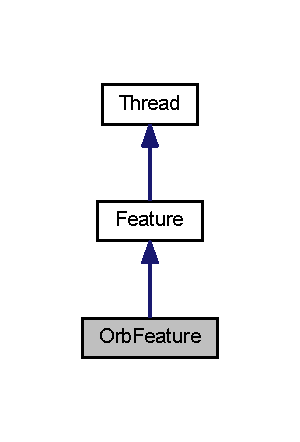
\includegraphics[height=550pt]{class_orb_feature__inherit__graph}
\end{center}
\end{figure}


Collaboration diagram for Orb\-Feature\-:
\nopagebreak
\begin{figure}[H]
\begin{center}
\leavevmode
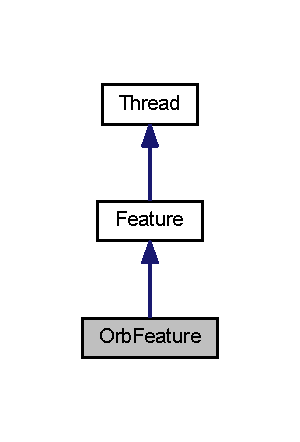
\includegraphics[height=550pt]{class_orb_feature__coll__graph}
\end{center}
\end{figure}
\subsubsection*{Public Member Functions}
\begin{DoxyCompactItemize}
\item 
\hyperlink{group___feature_extractor_aa6033d809df476d6798cf5f78fde25f7}{Orb\-Feature} (const std\-::string \&name, const std\-::string \&type)
\begin{DoxyCompactList}\small\item\em Constructor. \end{DoxyCompactList}\item 
\hyperlink{group___feature_extractor_aed4e5d5b4410041d3c8374dbd929f2ef}{$\sim$\-Orb\-Feature} (void)
\begin{DoxyCompactList}\small\item\em Destructor. \end{DoxyCompactList}\item 
const std\-::string \& \hyperlink{group___feature_extractor_a5f69ca2455d5eec4493dbf115d00d5c9}{Get\-Name} (void)
\begin{DoxyCompactList}\small\item\em Name getter. \end{DoxyCompactList}\item 
double \hyperlink{group___feature_extractor_ad07a3104192b50d911eee634a0be009d}{Get\-Proc\-Time} (void)
\begin{DoxyCompactList}\small\item\em Process time getter. \end{DoxyCompactList}\item 
const std\-::string \& \hyperlink{group___feature_extractor_a6724c19006d495bd6a9c8c6029236ebc}{Get\-Type} (void)
\begin{DoxyCompactList}\small\item\em Type getter. \end{DoxyCompactList}\item 
void $\ast$ \hyperlink{group___core_a8f33f7750321d5df9188033e7e3e300d}{Join} (void)
\item 
void \hyperlink{group___feature_extractor_aa13ad1fbc5869dcabb55611e5c206ebd}{Load\-Settings\-From\-File\-Storage} (void)
\begin{DoxyCompactList}\small\item\em Implemented virtual method for loading algorithm specific settings from the given storage. \end{DoxyCompactList}\item 
void \hyperlink{group___feature_extractor_a3c58d995fb2440b28db3b21b54b94815}{Set\-Frame} (const cv\-::\-Mat \&frame)
\begin{DoxyCompactList}\small\item\em Connects a frame to the feature extractor. \end{DoxyCompactList}\item 
void \hyperlink{group___core_a2b42f82341afd2747ea093b6ac8b91cb}{Start} (void)
\begin{DoxyCompactList}\small\item\em Starts the thread. \end{DoxyCompactList}\end{DoxyCompactItemize}
\subsubsection*{Public Attributes}
\begin{DoxyCompactItemize}
\item 
std\-::vector$<$ cv\-::\-Key\-Point $>$ \hyperlink{group___feature_extractor_a72cc606c0090a64718a7e92bca7520b9}{key\-Points}
\begin{DoxyCompactList}\small\item\em Stores keypoints, i.\-e. a point feature found by one of many available keypoint detectors. \end{DoxyCompactList}\end{DoxyCompactItemize}
\subsubsection*{Protected Attributes}
\begin{DoxyCompactItemize}
\item 
cv\-::\-Mat \hyperlink{group___feature_extractor_aae4295da2c3999edcb99b46d70ee7166}{frame\-\_\-}
\begin{DoxyCompactList}\small\item\em The current frame. \end{DoxyCompactList}\item 
std\-::string \hyperlink{group___feature_extractor_abee52be830de272bd27685083bf28aae}{name\-\_\-}
\begin{DoxyCompactList}\small\item\em Name of the current feature extraction procedure. \end{DoxyCompactList}\item 
double \hyperlink{group___feature_extractor_aa3306975b929f5503dac51829f9e04a0}{proc\-Time\-\_\-}
\begin{DoxyCompactList}\small\item\em Processing time of the current feature extraction method. \end{DoxyCompactList}\item 
std\-::string \hyperlink{group___feature_extractor_ad467857c4bc3d0fe65ba29e3b8f7c796}{type\-\_\-}
\begin{DoxyCompactList}\small\item\em Type of the current feature extraction procedure. \end{DoxyCompactList}\end{DoxyCompactItemize}
\subsubsection*{Private Member Functions}
\begin{DoxyCompactItemize}
\item 
void \hyperlink{group___feature_extractor_a907fdd9790d0295f129f1ecdc4382031}{Draw\-Features} (void)
\begin{DoxyCompactList}\small\item\em Implemented virtual method for displaying the output. \end{DoxyCompactList}\item 
void \hyperlink{group___feature_extractor_af814e3440b61e6bf13b44ef8886ad2d0}{Process} (void)
\begin{DoxyCompactList}\small\item\em Implemented virtual method for the algorithm. \end{DoxyCompactList}\end{DoxyCompactItemize}
\subsubsection*{Private Attributes}
\begin{DoxyCompactItemize}
\item 
int \hyperlink{group___feature_extractor_af74609fa7b56d5dea19c9460f42b25ab}{edge\-Threshold\-\_\-}
\begin{DoxyCompactList}\small\item\em This is size of the border where the features are not detected. It should roughly match the patch\-Size parameter. \end{DoxyCompactList}\item 
int \hyperlink{group___feature_extractor_a1c1e186a9f2bc54c38f54f3c1e8f7d0f}{first\-Level\-\_\-}
\begin{DoxyCompactList}\small\item\em It should be 0 in the current implementation. \end{DoxyCompactList}\item 
int \hyperlink{group___feature_extractor_a8fb8ef05ff3dff5ffee90c6f41e83cb2}{n\-Features\-\_\-}
\begin{DoxyCompactList}\small\item\em The maximum number of features to retain. \end{DoxyCompactList}\item 
int \hyperlink{group___feature_extractor_abfb07330bd1a63270f935e1317111300}{nlevels\-\_\-}
\begin{DoxyCompactList}\small\item\em The number of pyramid levels. The smallest level will have linear size equal to input\-\_\-image\-\_\-linear\-\_\-size/pow(scale\-Factor, nlevels). \end{DoxyCompactList}\item 
cv\-::\-Orb\-Feature\-Detector $\ast$ \hyperlink{group___feature_extractor_afbddce112b372099591a6ec049aff0f5}{orb\-Detector\-\_\-}
\begin{DoxyCompactList}\small\item\em Wrapped Open\-C\-V O\-R\-B object. \end{DoxyCompactList}\item 
int \hyperlink{group___feature_extractor_ae7f8a68d8b86f650348bc213c43f593a}{patch\-Size\-\_\-}
\begin{DoxyCompactList}\small\item\em Size of the patch used by the oriented B\-R\-I\-E\-F descriptor. Of course, on smaller pyramid layers the perceived image area covered by a feature will be larger. \end{DoxyCompactList}\item 
float \hyperlink{group___feature_extractor_a8cbd44d79e8952dd7b51be32d1eaddee}{scale\-Factor\-\_\-}
\begin{DoxyCompactList}\small\item\em Pyramid decimation ratio, greater than 1. scale\-Factor==2 means the classical pyramid, where each next level has 4x less pixels than the previous, but such a big scale factor will degrade feature matching scores dramatically. On the other hand, too close to 1 scale factor will mean that to cover certain scale range you will need more pyramid levels and so the speed will suffer. \end{DoxyCompactList}\item 
int \hyperlink{group___feature_extractor_a9a4454ef09254b94d88d0b599ad84218}{score\-Type\-\_\-}
\begin{DoxyCompactList}\small\item\em he default H\-A\-R\-R\-I\-S\-\_\-\-S\-C\-O\-R\-E means that Harris algorithm is used to rank features (the score is written to Key\-Point\-::score and is used to retain best nfeatures features); F\-A\-S\-T\-\_\-\-S\-C\-O\-R\-E is alternative value of the parameter that produces slightly less stable keypoints, but it is a little faster to compute. \end{DoxyCompactList}\item 
int \hyperlink{group___feature_extractor_a05cc269e6833e1f25c7f7c31928a5ef6}{wta\-K\-\_\-}
\begin{DoxyCompactList}\small\item\em The number of points that produce each element of the oriented B\-R\-I\-E\-F descriptor. The default value 2 means the B\-R\-I\-E\-F where we take a random point pair and compare their brightnesses, so we get 0/1 response. Other possible values are 3 and 4. For example, 3 means that we take 3 random points (of course, those point coordinates are random, but they are generated from the pre-\/defined seed, so each element of B\-R\-I\-E\-F descriptor is computed deterministically from the pixel rectangle), find point of maximum brightness and output index of the winner (0, 1 or 2). Such output will occupy 2 bits, and therefore it will need a special variant of Hamming distance, denoted as N\-O\-R\-M\-\_\-\-H\-A\-M\-M\-I\-N\-G2 (2 bits per bin). When W\-T\-A\-\_\-\-K=4, we take 4 random points to compute each bin (that will also occupy 2 bits with possible values 0, 1, 2 or 3). \end{DoxyCompactList}\end{DoxyCompactItemize}


\paragraph{Constructor \& Destructor Documentation}
\hypertarget{group___feature_extractor_aa6033d809df476d6798cf5f78fde25f7}{\index{Orb\-Feature@{Orb\-Feature}!Orb\-Feature@{Orb\-Feature}}
\index{Orb\-Feature@{Orb\-Feature}!OrbFeature@{Orb\-Feature}}
\subparagraph[{Orb\-Feature}]{\setlength{\rightskip}{0pt plus 5cm}Orb\-Feature\-::\-Orb\-Feature (
\begin{DoxyParamCaption}
\item[{const std\-::string \&}]{name, }
\item[{const std\-::string \&}]{type}
\end{DoxyParamCaption}
)}}\label{group___feature_extractor_aa6033d809df476d6798cf5f78fde25f7}


Constructor. 

\begin{DoxyVerb}    \param name Name of the current feature extraction procedure.
\end{DoxyVerb}
 
\begin{DoxyParams}{Parameters}
{\em type} & Type of the current feature extraction procedure (global or local). \\
\hline
\end{DoxyParams}


References edge\-Threshold\-\_\-, first\-Level\-\_\-, Load\-Settings\-From\-File\-Storage(), n\-Features\-\_\-, nlevels\-\_\-, orb\-Detector\-\_\-, patch\-Size\-\_\-, scale\-Factor\-\_\-, score\-Type\-\_\-, and wta\-K\-\_\-.



Here is the call graph for this function\-:
\nopagebreak
\begin{figure}[H]
\begin{center}
\leavevmode
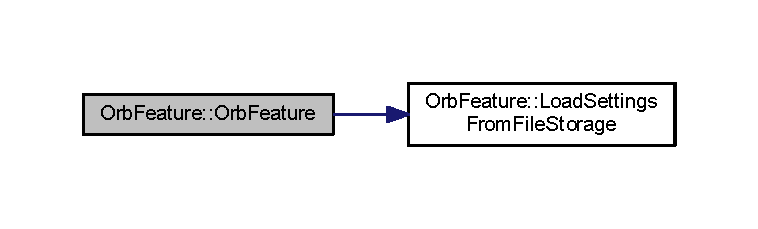
\includegraphics[width=350pt]{group___feature_extractor_aa6033d809df476d6798cf5f78fde25f7_cgraph}
\end{center}
\end{figure}


\hypertarget{group___feature_extractor_aed4e5d5b4410041d3c8374dbd929f2ef}{\index{Orb\-Feature@{Orb\-Feature}!$\sim$\-Orb\-Feature@{$\sim$\-Orb\-Feature}}
\index{$\sim$\-Orb\-Feature@{$\sim$\-Orb\-Feature}!OrbFeature@{Orb\-Feature}}
\subparagraph[{$\sim$\-Orb\-Feature}]{\setlength{\rightskip}{0pt plus 5cm}Orb\-Feature\-::$\sim$\-Orb\-Feature (
\begin{DoxyParamCaption}
\item[{void}]{}
\end{DoxyParamCaption}
)}}\label{group___feature_extractor_aed4e5d5b4410041d3c8374dbd929f2ef}


Destructor. 



References orb\-Detector\-\_\-.



\paragraph{Member Function Documentation}
\hypertarget{group___feature_extractor_a907fdd9790d0295f129f1ecdc4382031}{\index{Orb\-Feature@{Orb\-Feature}!Draw\-Features@{Draw\-Features}}
\index{Draw\-Features@{Draw\-Features}!OrbFeature@{Orb\-Feature}}
\subparagraph[{Draw\-Features}]{\setlength{\rightskip}{0pt plus 5cm}void Orb\-Feature\-::\-Draw\-Features (
\begin{DoxyParamCaption}
\item[{void}]{}
\end{DoxyParamCaption}
)\hspace{0.3cm}{\ttfamily [private]}, {\ttfamily [virtual]}}}\label{group___feature_extractor_a907fdd9790d0295f129f1ecdc4382031}


Implemented virtual method for displaying the output. 

\begin{DoxySeeAlso}{See Also}
\hyperlink{group___feature_extractor_acea1ee12c177894819ea7ae0f6294e5c}{Global\-Feature\-::\-Draw\-Features()} 
\end{DoxySeeAlso}


Reimplemented from \hyperlink{group___feature_extractor_acea1ee12c177894819ea7ae0f6294e5c}{Global\-Feature}.



References Global\-Feature\-::frame\-\_\-, and Global\-Feature\-::key\-Points.

\hypertarget{group___feature_extractor_a5f69ca2455d5eec4493dbf115d00d5c9}{\index{Orb\-Feature@{Orb\-Feature}!Get\-Name@{Get\-Name}}
\index{Get\-Name@{Get\-Name}!OrbFeature@{Orb\-Feature}}
\subparagraph[{Get\-Name}]{\setlength{\rightskip}{0pt plus 5cm}const string \& Global\-Feature\-::\-Get\-Name (
\begin{DoxyParamCaption}
\item[{void}]{}
\end{DoxyParamCaption}
)\hspace{0.3cm}{\ttfamily [inherited]}}}\label{group___feature_extractor_a5f69ca2455d5eec4493dbf115d00d5c9}


Name getter. 

\begin{DoxyReturn}{Returns}
Name of the current feature extraction procedure. 
\end{DoxyReturn}


References Global\-Feature\-::name\-\_\-.

\hypertarget{group___feature_extractor_ad07a3104192b50d911eee634a0be009d}{\index{Orb\-Feature@{Orb\-Feature}!Get\-Proc\-Time@{Get\-Proc\-Time}}
\index{Get\-Proc\-Time@{Get\-Proc\-Time}!OrbFeature@{Orb\-Feature}}
\subparagraph[{Get\-Proc\-Time}]{\setlength{\rightskip}{0pt plus 5cm}double Global\-Feature\-::\-Get\-Proc\-Time (
\begin{DoxyParamCaption}
\item[{void}]{}
\end{DoxyParamCaption}
)\hspace{0.3cm}{\ttfamily [inherited]}}}\label{group___feature_extractor_ad07a3104192b50d911eee634a0be009d}


Process time getter. 

\begin{DoxyReturn}{Returns}
Processing time of the current feature extraction method. 
\end{DoxyReturn}


References Global\-Feature\-::proc\-Time\-\_\-.

\hypertarget{group___feature_extractor_a6724c19006d495bd6a9c8c6029236ebc}{\index{Orb\-Feature@{Orb\-Feature}!Get\-Type@{Get\-Type}}
\index{Get\-Type@{Get\-Type}!OrbFeature@{Orb\-Feature}}
\subparagraph[{Get\-Type}]{\setlength{\rightskip}{0pt plus 5cm}const string \& Global\-Feature\-::\-Get\-Type (
\begin{DoxyParamCaption}
\item[{void}]{}
\end{DoxyParamCaption}
)\hspace{0.3cm}{\ttfamily [inherited]}}}\label{group___feature_extractor_a6724c19006d495bd6a9c8c6029236ebc}


Type getter. 

\begin{DoxyReturn}{Returns}
Type of the current feature extraction procedure. 
\end{DoxyReturn}


References Global\-Feature\-::type\-\_\-.

\hypertarget{group___core_a8f33f7750321d5df9188033e7e3e300d}{\index{Orb\-Feature@{Orb\-Feature}!Join@{Join}}
\index{Join@{Join}!OrbFeature@{Orb\-Feature}}
\subparagraph[{Join}]{\setlength{\rightskip}{0pt plus 5cm}void $\ast$ Thread\-::\-Join (
\begin{DoxyParamCaption}
\item[{void}]{}
\end{DoxyParamCaption}
)\hspace{0.3cm}{\ttfamily [inherited]}}}\label{group___core_a8f33f7750321d5df9188033e7e3e300d}


References Exception\-Error, Thread\-::result\-\_\-, and Thread\-::thread\-I\-D\-\_\-.

\hypertarget{group___feature_extractor_aa13ad1fbc5869dcabb55611e5c206ebd}{\index{Orb\-Feature@{Orb\-Feature}!Load\-Settings\-From\-File\-Storage@{Load\-Settings\-From\-File\-Storage}}
\index{Load\-Settings\-From\-File\-Storage@{Load\-Settings\-From\-File\-Storage}!OrbFeature@{Orb\-Feature}}
\subparagraph[{Load\-Settings\-From\-File\-Storage}]{\setlength{\rightskip}{0pt plus 5cm}void Orb\-Feature\-::\-Load\-Settings\-From\-File\-Storage (
\begin{DoxyParamCaption}
\item[{void}]{}
\end{DoxyParamCaption}
)\hspace{0.3cm}{\ttfamily [virtual]}}}\label{group___feature_extractor_aa13ad1fbc5869dcabb55611e5c206ebd}


Implemented virtual method for loading algorithm specific settings from the given storage. 

\begin{DoxySeeAlso}{See Also}
\hyperlink{group___feature_extractor_aa48133762d9f52a5c2ae5042f6ebbe71}{Global\-Feature\-::\-Load\-Settings\-From\-File\-Storage()} 
\end{DoxySeeAlso}


Reimplemented from \hyperlink{group___feature_extractor_aa48133762d9f52a5c2ae5042f6ebbe71}{Global\-Feature}.



References edge\-Threshold\-\_\-, Exception\-Error, first\-Level\-\_\-, Local\-Settings\-Ptr, Global\-Feature\-::name\-\_\-, n\-Features\-\_\-, nlevels\-\_\-, patch\-Size\-\_\-, scale\-Factor\-\_\-, score\-Type\-\_\-, and wta\-K\-\_\-.



Referenced by Orb\-Feature().



Here is the caller graph for this function\-:
\nopagebreak
\begin{figure}[H]
\begin{center}
\leavevmode
\includegraphics[width=350pt]{group___feature_extractor_aa13ad1fbc5869dcabb55611e5c206ebd_icgraph}
\end{center}
\end{figure}


\hypertarget{group___feature_extractor_af814e3440b61e6bf13b44ef8886ad2d0}{\index{Orb\-Feature@{Orb\-Feature}!Process@{Process}}
\index{Process@{Process}!OrbFeature@{Orb\-Feature}}
\subparagraph[{Process}]{\setlength{\rightskip}{0pt plus 5cm}void Orb\-Feature\-::\-Process (
\begin{DoxyParamCaption}
\item[{void}]{}
\end{DoxyParamCaption}
)\hspace{0.3cm}{\ttfamily [private]}, {\ttfamily [virtual]}}}\label{group___feature_extractor_af814e3440b61e6bf13b44ef8886ad2d0}


Implemented virtual method for the algorithm. 

\begin{DoxySeeAlso}{See Also}
\hyperlink{group___feature_extractor_a9fdfc934c5a9da6962ec39c1b0cf32dc}{Global\-Feature\-::\-Process()} 
\end{DoxySeeAlso}


Reimplemented from \hyperlink{group___feature_extractor_a9fdfc934c5a9da6962ec39c1b0cf32dc}{Global\-Feature}.



References Global\-Feature\-::frame\-\_\-, Global\-Feature\-::key\-Points, and orb\-Detector\-\_\-.

\hypertarget{group___feature_extractor_a3c58d995fb2440b28db3b21b54b94815}{\index{Orb\-Feature@{Orb\-Feature}!Set\-Frame@{Set\-Frame}}
\index{Set\-Frame@{Set\-Frame}!OrbFeature@{Orb\-Feature}}
\subparagraph[{Set\-Frame}]{\setlength{\rightskip}{0pt plus 5cm}void Global\-Feature\-::\-Set\-Frame (
\begin{DoxyParamCaption}
\item[{const cv\-::\-Mat \&}]{frame}
\end{DoxyParamCaption}
)\hspace{0.3cm}{\ttfamily [inherited]}}}\label{group___feature_extractor_a3c58d995fb2440b28db3b21b54b94815}


Connects a frame to the feature extractor. 


\begin{DoxyParams}{Parameters}
{\em frame} & Output parameter for the current frame. \\
\hline
\end{DoxyParams}


References Global\-Feature\-::frame\-\_\-.

\hypertarget{group___core_a2b42f82341afd2747ea093b6ac8b91cb}{\index{Orb\-Feature@{Orb\-Feature}!Start@{Start}}
\index{Start@{Start}!OrbFeature@{Orb\-Feature}}
\subparagraph[{Start}]{\setlength{\rightskip}{0pt plus 5cm}void Thread\-::\-Start (
\begin{DoxyParamCaption}
\item[{void}]{}
\end{DoxyParamCaption}
)\hspace{0.3cm}{\ttfamily [inherited]}}}\label{group___core_a2b42f82341afd2747ea093b6ac8b91cb}


Starts the thread. 



References Thread\-::detached\-\_\-, Exception\-Error, Thread\-::runnable\-\_\-, Thread\-::\-Start\-Thread(), Thread\-::\-Start\-Thread\-Runnable(), Thread\-::thread\-Attribute\-\_\-, and Thread\-::thread\-I\-D\-\_\-.



Here is the call graph for this function\-:
\nopagebreak
\begin{figure}[H]
\begin{center}
\leavevmode
\includegraphics[width=350pt]{group___core_a2b42f82341afd2747ea093b6ac8b91cb_cgraph}
\end{center}
\end{figure}




\paragraph{Member Data Documentation}
\hypertarget{group___feature_extractor_af74609fa7b56d5dea19c9460f42b25ab}{\index{Orb\-Feature@{Orb\-Feature}!edge\-Threshold\-\_\-@{edge\-Threshold\-\_\-}}
\index{edge\-Threshold\-\_\-@{edge\-Threshold\-\_\-}!OrbFeature@{Orb\-Feature}}
\subparagraph[{edge\-Threshold\-\_\-}]{\setlength{\rightskip}{0pt plus 5cm}int Orb\-Feature\-::edge\-Threshold\-\_\-\hspace{0.3cm}{\ttfamily [private]}}}\label{group___feature_extractor_af74609fa7b56d5dea19c9460f42b25ab}


This is size of the border where the features are not detected. It should roughly match the patch\-Size parameter. 



Referenced by Load\-Settings\-From\-File\-Storage(), and Orb\-Feature().

\hypertarget{group___feature_extractor_a1c1e186a9f2bc54c38f54f3c1e8f7d0f}{\index{Orb\-Feature@{Orb\-Feature}!first\-Level\-\_\-@{first\-Level\-\_\-}}
\index{first\-Level\-\_\-@{first\-Level\-\_\-}!OrbFeature@{Orb\-Feature}}
\subparagraph[{first\-Level\-\_\-}]{\setlength{\rightskip}{0pt plus 5cm}int Orb\-Feature\-::first\-Level\-\_\-\hspace{0.3cm}{\ttfamily [private]}}}\label{group___feature_extractor_a1c1e186a9f2bc54c38f54f3c1e8f7d0f}


It should be 0 in the current implementation. 



Referenced by Load\-Settings\-From\-File\-Storage(), and Orb\-Feature().

\hypertarget{group___feature_extractor_aae4295da2c3999edcb99b46d70ee7166}{\index{Orb\-Feature@{Orb\-Feature}!frame\-\_\-@{frame\-\_\-}}
\index{frame\-\_\-@{frame\-\_\-}!OrbFeature@{Orb\-Feature}}
\subparagraph[{frame\-\_\-}]{\setlength{\rightskip}{0pt plus 5cm}cv\-::\-Mat Global\-Feature\-::frame\-\_\-\hspace{0.3cm}{\ttfamily [protected]}, {\ttfamily [inherited]}}}\label{group___feature_extractor_aae4295da2c3999edcb99b46d70ee7166}


The current frame. 



Referenced by Mser\-Feature\-::\-Draw\-Features(), Star\-Feature\-::\-Draw\-Features(), Draw\-Features(), Sift\-Feature\-::\-Draw\-Features(), Fast\-Feature\-::\-Draw\-Features(), Surf\-Feature\-::\-Draw\-Features(), Mser\-Feature\-::\-Process(), Star\-Feature\-::\-Process(), Fast\-Feature\-::\-Process(), Surf\-Feature\-::\-Process(), Process(), Sift\-Feature\-::\-Process(), Global\-Feature\-::\-Run(), Global\-Feature\-::\-Set\-Frame(), and Global\-Feature\-::\-Visualize().

\hypertarget{group___feature_extractor_a72cc606c0090a64718a7e92bca7520b9}{\index{Orb\-Feature@{Orb\-Feature}!key\-Points@{key\-Points}}
\index{key\-Points@{key\-Points}!OrbFeature@{Orb\-Feature}}
\subparagraph[{key\-Points}]{\setlength{\rightskip}{0pt plus 5cm}std\-::vector$<$cv\-::\-Key\-Point$>$ Global\-Feature\-::key\-Points\hspace{0.3cm}{\ttfamily [inherited]}}}\label{group___feature_extractor_a72cc606c0090a64718a7e92bca7520b9}


Stores keypoints, i.\-e. a point feature found by one of many available keypoint detectors. 



Referenced by Mser\-Feature\-::\-Draw\-Features(), Star\-Feature\-::\-Draw\-Features(), Sift\-Feature\-::\-Draw\-Features(), Fast\-Feature\-::\-Draw\-Features(), Draw\-Features(), Surf\-Feature\-::\-Draw\-Features(), Star\-Feature\-::\-Process(), Mser\-Feature\-::\-Process(), Process(), Sift\-Feature\-::\-Process(), Surf\-Feature\-::\-Process(), Fast\-Feature\-::\-Process(), and Global\-Feature\-::\-Visualize().

\hypertarget{group___feature_extractor_abee52be830de272bd27685083bf28aae}{\index{Orb\-Feature@{Orb\-Feature}!name\-\_\-@{name\-\_\-}}
\index{name\-\_\-@{name\-\_\-}!OrbFeature@{Orb\-Feature}}
\subparagraph[{name\-\_\-}]{\setlength{\rightskip}{0pt plus 5cm}std\-::string Global\-Feature\-::name\-\_\-\hspace{0.3cm}{\ttfamily [protected]}, {\ttfamily [inherited]}}}\label{group___feature_extractor_abee52be830de272bd27685083bf28aae}


Name of the current feature extraction procedure. 



Referenced by Global\-Feature\-::\-Get\-Name(), Mser\-Feature\-::\-Load\-Settings\-From\-File\-Storage(), Star\-Feature\-::\-Load\-Settings\-From\-File\-Storage(), Surf\-Feature\-::\-Load\-Settings\-From\-File\-Storage(), Load\-Settings\-From\-File\-Storage(), Sift\-Feature\-::\-Load\-Settings\-From\-File\-Storage(), Fast\-Feature\-::\-Load\-Settings\-From\-File\-Storage(), and Global\-Feature\-::\-Visualize().

\hypertarget{group___feature_extractor_a8fb8ef05ff3dff5ffee90c6f41e83cb2}{\index{Orb\-Feature@{Orb\-Feature}!n\-Features\-\_\-@{n\-Features\-\_\-}}
\index{n\-Features\-\_\-@{n\-Features\-\_\-}!OrbFeature@{Orb\-Feature}}
\subparagraph[{n\-Features\-\_\-}]{\setlength{\rightskip}{0pt plus 5cm}int Orb\-Feature\-::n\-Features\-\_\-\hspace{0.3cm}{\ttfamily [private]}}}\label{group___feature_extractor_a8fb8ef05ff3dff5ffee90c6f41e83cb2}


The maximum number of features to retain. 



Referenced by Load\-Settings\-From\-File\-Storage(), and Orb\-Feature().

\hypertarget{group___feature_extractor_abfb07330bd1a63270f935e1317111300}{\index{Orb\-Feature@{Orb\-Feature}!nlevels\-\_\-@{nlevels\-\_\-}}
\index{nlevels\-\_\-@{nlevels\-\_\-}!OrbFeature@{Orb\-Feature}}
\subparagraph[{nlevels\-\_\-}]{\setlength{\rightskip}{0pt plus 5cm}int Orb\-Feature\-::nlevels\-\_\-\hspace{0.3cm}{\ttfamily [private]}}}\label{group___feature_extractor_abfb07330bd1a63270f935e1317111300}


The number of pyramid levels. The smallest level will have linear size equal to input\-\_\-image\-\_\-linear\-\_\-size/pow(scale\-Factor, nlevels). 



Referenced by Load\-Settings\-From\-File\-Storage(), and Orb\-Feature().

\hypertarget{group___feature_extractor_afbddce112b372099591a6ec049aff0f5}{\index{Orb\-Feature@{Orb\-Feature}!orb\-Detector\-\_\-@{orb\-Detector\-\_\-}}
\index{orb\-Detector\-\_\-@{orb\-Detector\-\_\-}!OrbFeature@{Orb\-Feature}}
\subparagraph[{orb\-Detector\-\_\-}]{\setlength{\rightskip}{0pt plus 5cm}cv\-::\-Orb\-Feature\-Detector$\ast$ Orb\-Feature\-::orb\-Detector\-\_\-\hspace{0.3cm}{\ttfamily [private]}}}\label{group___feature_extractor_afbddce112b372099591a6ec049aff0f5}


Wrapped Open\-C\-V O\-R\-B object. 



Referenced by Orb\-Feature(), Process(), and $\sim$\-Orb\-Feature().

\hypertarget{group___feature_extractor_ae7f8a68d8b86f650348bc213c43f593a}{\index{Orb\-Feature@{Orb\-Feature}!patch\-Size\-\_\-@{patch\-Size\-\_\-}}
\index{patch\-Size\-\_\-@{patch\-Size\-\_\-}!OrbFeature@{Orb\-Feature}}
\subparagraph[{patch\-Size\-\_\-}]{\setlength{\rightskip}{0pt plus 5cm}int Orb\-Feature\-::patch\-Size\-\_\-\hspace{0.3cm}{\ttfamily [private]}}}\label{group___feature_extractor_ae7f8a68d8b86f650348bc213c43f593a}


Size of the patch used by the oriented B\-R\-I\-E\-F descriptor. Of course, on smaller pyramid layers the perceived image area covered by a feature will be larger. 



Referenced by Load\-Settings\-From\-File\-Storage(), and Orb\-Feature().

\hypertarget{group___feature_extractor_aa3306975b929f5503dac51829f9e04a0}{\index{Orb\-Feature@{Orb\-Feature}!proc\-Time\-\_\-@{proc\-Time\-\_\-}}
\index{proc\-Time\-\_\-@{proc\-Time\-\_\-}!OrbFeature@{Orb\-Feature}}
\subparagraph[{proc\-Time\-\_\-}]{\setlength{\rightskip}{0pt plus 5cm}double Global\-Feature\-::proc\-Time\-\_\-\hspace{0.3cm}{\ttfamily [protected]}, {\ttfamily [inherited]}}}\label{group___feature_extractor_aa3306975b929f5503dac51829f9e04a0}


Processing time of the current feature extraction method. 



Referenced by Global\-Feature\-::\-Get\-Proc\-Time(), Global\-Feature\-::\-Run(), and Global\-Feature\-::\-Visualize().

\hypertarget{group___feature_extractor_a8cbd44d79e8952dd7b51be32d1eaddee}{\index{Orb\-Feature@{Orb\-Feature}!scale\-Factor\-\_\-@{scale\-Factor\-\_\-}}
\index{scale\-Factor\-\_\-@{scale\-Factor\-\_\-}!OrbFeature@{Orb\-Feature}}
\subparagraph[{scale\-Factor\-\_\-}]{\setlength{\rightskip}{0pt plus 5cm}float Orb\-Feature\-::scale\-Factor\-\_\-\hspace{0.3cm}{\ttfamily [private]}}}\label{group___feature_extractor_a8cbd44d79e8952dd7b51be32d1eaddee}


Pyramid decimation ratio, greater than 1. scale\-Factor==2 means the classical pyramid, where each next level has 4x less pixels than the previous, but such a big scale factor will degrade feature matching scores dramatically. On the other hand, too close to 1 scale factor will mean that to cover certain scale range you will need more pyramid levels and so the speed will suffer. 



Referenced by Load\-Settings\-From\-File\-Storage(), and Orb\-Feature().

\hypertarget{group___feature_extractor_a9a4454ef09254b94d88d0b599ad84218}{\index{Orb\-Feature@{Orb\-Feature}!score\-Type\-\_\-@{score\-Type\-\_\-}}
\index{score\-Type\-\_\-@{score\-Type\-\_\-}!OrbFeature@{Orb\-Feature}}
\subparagraph[{score\-Type\-\_\-}]{\setlength{\rightskip}{0pt plus 5cm}int Orb\-Feature\-::score\-Type\-\_\-\hspace{0.3cm}{\ttfamily [private]}}}\label{group___feature_extractor_a9a4454ef09254b94d88d0b599ad84218}


he default H\-A\-R\-R\-I\-S\-\_\-\-S\-C\-O\-R\-E means that Harris algorithm is used to rank features (the score is written to Key\-Point\-::score and is used to retain best nfeatures features); F\-A\-S\-T\-\_\-\-S\-C\-O\-R\-E is alternative value of the parameter that produces slightly less stable keypoints, but it is a little faster to compute. 



Referenced by Load\-Settings\-From\-File\-Storage(), and Orb\-Feature().

\hypertarget{group___feature_extractor_ad467857c4bc3d0fe65ba29e3b8f7c796}{\index{Orb\-Feature@{Orb\-Feature}!type\-\_\-@{type\-\_\-}}
\index{type\-\_\-@{type\-\_\-}!OrbFeature@{Orb\-Feature}}
\subparagraph[{type\-\_\-}]{\setlength{\rightskip}{0pt plus 5cm}std\-::string Global\-Feature\-::type\-\_\-\hspace{0.3cm}{\ttfamily [protected]}, {\ttfamily [inherited]}}}\label{group___feature_extractor_ad467857c4bc3d0fe65ba29e3b8f7c796}


Type of the current feature extraction procedure. 



Referenced by Global\-Feature\-::\-Get\-Type().

\hypertarget{group___feature_extractor_a05cc269e6833e1f25c7f7c31928a5ef6}{\index{Orb\-Feature@{Orb\-Feature}!wta\-K\-\_\-@{wta\-K\-\_\-}}
\index{wta\-K\-\_\-@{wta\-K\-\_\-}!OrbFeature@{Orb\-Feature}}
\subparagraph[{wta\-K\-\_\-}]{\setlength{\rightskip}{0pt plus 5cm}int Orb\-Feature\-::wta\-K\-\_\-\hspace{0.3cm}{\ttfamily [private]}}}\label{group___feature_extractor_a05cc269e6833e1f25c7f7c31928a5ef6}


The number of points that produce each element of the oriented B\-R\-I\-E\-F descriptor. The default value 2 means the B\-R\-I\-E\-F where we take a random point pair and compare their brightnesses, so we get 0/1 response. Other possible values are 3 and 4. For example, 3 means that we take 3 random points (of course, those point coordinates are random, but they are generated from the pre-\/defined seed, so each element of B\-R\-I\-E\-F descriptor is computed deterministically from the pixel rectangle), find point of maximum brightness and output index of the winner (0, 1 or 2). Such output will occupy 2 bits, and therefore it will need a special variant of Hamming distance, denoted as N\-O\-R\-M\-\_\-\-H\-A\-M\-M\-I\-N\-G2 (2 bits per bin). When W\-T\-A\-\_\-\-K=4, we take 4 random points to compute each bin (that will also occupy 2 bits with possible values 0, 1, 2 or 3). 



Referenced by Load\-Settings\-From\-File\-Storage(), and Orb\-Feature().

\index{Sift\-Feature@{Sift\-Feature}}\label{class_sift_feature}
\hypertarget{group___feature_extractor_class_sift_feature}{}
\subsubsection{class Sift\-Feature}
Class for extracting S\-I\-F\-T features. 

Class for extracting keypoints and computing descriptors using the Scale Invariant Feature Transform (S\-I\-F\-T) algorithm by D. Lowe.

See paper\-: Lowe, D. G., “\-Distinctive Image Features from Scale-\/\-Invariant Keypoints”, International Journal of Computer Vision, 60, 2, pp. 91-\/110, 2004. 

Inheritance diagram for Sift\-Feature\-:
\nopagebreak
\begin{figure}[H]
\begin{center}
\leavevmode
\includegraphics[height=550pt]{class_sift_feature__inherit__graph}
\end{center}
\end{figure}


Collaboration diagram for Sift\-Feature\-:
\nopagebreak
\begin{figure}[H]
\begin{center}
\leavevmode
\includegraphics[height=550pt]{class_sift_feature__coll__graph}
\end{center}
\end{figure}
\subsubsection*{Public Member Functions}
\begin{DoxyCompactItemize}
\item 
\hyperlink{group___feature_extractor_a9fc5b3a0395374f1bb07fad1ad9a2494}{Sift\-Feature} (const std\-::string \&name, const std\-::string \&type)
\begin{DoxyCompactList}\small\item\em Constructor. \end{DoxyCompactList}\item 
\hyperlink{group___feature_extractor_af35ea372a4c8aaf8a7486ec688214527}{$\sim$\-Sift\-Feature} (void)
\begin{DoxyCompactList}\small\item\em Destructor. \end{DoxyCompactList}\item 
const std\-::string \& \hyperlink{group___feature_extractor_a5f69ca2455d5eec4493dbf115d00d5c9}{Get\-Name} (void)
\begin{DoxyCompactList}\small\item\em Name getter. \end{DoxyCompactList}\item 
double \hyperlink{group___feature_extractor_ad07a3104192b50d911eee634a0be009d}{Get\-Proc\-Time} (void)
\begin{DoxyCompactList}\small\item\em Process time getter. \end{DoxyCompactList}\item 
const std\-::string \& \hyperlink{group___feature_extractor_a6724c19006d495bd6a9c8c6029236ebc}{Get\-Type} (void)
\begin{DoxyCompactList}\small\item\em Type getter. \end{DoxyCompactList}\item 
void $\ast$ \hyperlink{group___core_a8f33f7750321d5df9188033e7e3e300d}{Join} (void)
\item 
void \hyperlink{group___feature_extractor_af19316d789598f612ee150deb2ee5137}{Load\-Settings\-From\-File\-Storage} (void)
\begin{DoxyCompactList}\small\item\em Implemented virtual method for loading algorithm specific settings from the given storage. \end{DoxyCompactList}\item 
void \hyperlink{group___feature_extractor_a3c58d995fb2440b28db3b21b54b94815}{Set\-Frame} (const cv\-::\-Mat \&frame)
\begin{DoxyCompactList}\small\item\em Connects a frame to the feature extractor. \end{DoxyCompactList}\item 
void \hyperlink{group___core_a2b42f82341afd2747ea093b6ac8b91cb}{Start} (void)
\begin{DoxyCompactList}\small\item\em Starts the thread. \end{DoxyCompactList}\end{DoxyCompactItemize}
\subsubsection*{Public Attributes}
\begin{DoxyCompactItemize}
\item 
std\-::vector$<$ cv\-::\-Key\-Point $>$ \hyperlink{group___feature_extractor_a72cc606c0090a64718a7e92bca7520b9}{key\-Points}
\begin{DoxyCompactList}\small\item\em Stores keypoints, i.\-e. a point feature found by one of many available keypoint detectors. \end{DoxyCompactList}\end{DoxyCompactItemize}
\subsubsection*{Protected Attributes}
\begin{DoxyCompactItemize}
\item 
cv\-::\-Mat \hyperlink{group___feature_extractor_aae4295da2c3999edcb99b46d70ee7166}{frame\-\_\-}
\begin{DoxyCompactList}\small\item\em The current frame. \end{DoxyCompactList}\item 
std\-::string \hyperlink{group___feature_extractor_abee52be830de272bd27685083bf28aae}{name\-\_\-}
\begin{DoxyCompactList}\small\item\em Name of the current feature extraction procedure. \end{DoxyCompactList}\item 
double \hyperlink{group___feature_extractor_aa3306975b929f5503dac51829f9e04a0}{proc\-Time\-\_\-}
\begin{DoxyCompactList}\small\item\em Processing time of the current feature extraction method. \end{DoxyCompactList}\item 
std\-::string \hyperlink{group___feature_extractor_ad467857c4bc3d0fe65ba29e3b8f7c796}{type\-\_\-}
\begin{DoxyCompactList}\small\item\em Type of the current feature extraction procedure. \end{DoxyCompactList}\end{DoxyCompactItemize}
\subsubsection*{Private Member Functions}
\begin{DoxyCompactItemize}
\item 
void \hyperlink{group___feature_extractor_ae82e144ac3fed861dc0770cefaa828a6}{Draw\-Features} (void)
\begin{DoxyCompactList}\small\item\em Implemented virtual method for displaying the output. \end{DoxyCompactList}\item 
void \hyperlink{group___feature_extractor_a73513198ca8ff4e56be059521cfb60f5}{Process} (void)
\begin{DoxyCompactList}\small\item\em Implemented virtual method for the algorithm. \end{DoxyCompactList}\end{DoxyCompactItemize}
\subsubsection*{Private Attributes}
\begin{DoxyCompactItemize}
\item 
double \hyperlink{group___feature_extractor_af2a77eef4388e7b3504142218baee770}{contrast\-Threshold\-\_\-}
\begin{DoxyCompactList}\small\item\em The contrast threshold used to filter out weak features in semi-\/uniform (low-\/contrast) regions. The larger the threshold, the less features are produced by the detector. \end{DoxyCompactList}\item 
double \hyperlink{group___feature_extractor_a8fc64eb5826c05c5fe8c0893cc24ff0a}{edge\-Threshold\-\_\-}
\begin{DoxyCompactList}\small\item\em The threshold used to filter out edge-\/like features. Note that the its meaning is different from the contrast\-Threshold, i.\-e. the larger the edge\-Threshold, the less features are filtered out (more features are retained). \end{DoxyCompactList}\item 
int \hyperlink{group___feature_extractor_a7b777845234b488ea905bd38f7ce323c}{nfeatures\-\_\-}
\begin{DoxyCompactList}\small\item\em The number of best features to retain. The features are ranked by their scores (measured in S\-I\-F\-T algorithm as the local contrast). \end{DoxyCompactList}\item 
int \hyperlink{group___feature_extractor_aaf3149accfb0860cb148ea21cda53c12}{n\-Octave\-Layers\-\_\-}
\begin{DoxyCompactList}\small\item\em The number of layers in each octave. 3 is the value used in D. Lowe paper. The number of octaves is computed automatically from the image resolution. \end{DoxyCompactList}\item 
cv\-::\-Sift\-Feature\-Detector $\ast$ \hyperlink{group___feature_extractor_a4e08df2e30da758a11d029eae0352cf5}{sift\-Detector\-\_\-}
\begin{DoxyCompactList}\small\item\em Wrapped Open\-C\-V S\-I\-F\-T object. \end{DoxyCompactList}\item 
double \hyperlink{group___feature_extractor_a574fb46dbb906801014beb9a731b980a}{sigma\-\_\-}
\begin{DoxyCompactList}\small\item\em The sigma of the Gaussian applied to the input image at the octave \#0. If your image is captured with a weak camera with soft lenses, you might want to reduce the number. \end{DoxyCompactList}\end{DoxyCompactItemize}


\paragraph{Constructor \& Destructor Documentation}
\hypertarget{group___feature_extractor_a9fc5b3a0395374f1bb07fad1ad9a2494}{\index{Sift\-Feature@{Sift\-Feature}!Sift\-Feature@{Sift\-Feature}}
\index{Sift\-Feature@{Sift\-Feature}!SiftFeature@{Sift\-Feature}}
\subparagraph[{Sift\-Feature}]{\setlength{\rightskip}{0pt plus 5cm}Sift\-Feature\-::\-Sift\-Feature (
\begin{DoxyParamCaption}
\item[{const std\-::string \&}]{name, }
\item[{const std\-::string \&}]{type}
\end{DoxyParamCaption}
)}}\label{group___feature_extractor_a9fc5b3a0395374f1bb07fad1ad9a2494}


Constructor. 

\begin{DoxyVerb}    \param name Name of the current feature extraction procedure.
\end{DoxyVerb}
 
\begin{DoxyParams}{Parameters}
{\em type} & Type of the current feature extraction procedure (global or local). \\
\hline
\end{DoxyParams}


References contrast\-Threshold\-\_\-, edge\-Threshold\-\_\-, Load\-Settings\-From\-File\-Storage(), nfeatures\-\_\-, n\-Octave\-Layers\-\_\-, sift\-Detector\-\_\-, and sigma\-\_\-.



Here is the call graph for this function\-:
\nopagebreak
\begin{figure}[H]
\begin{center}
\leavevmode
\includegraphics[width=350pt]{group___feature_extractor_a9fc5b3a0395374f1bb07fad1ad9a2494_cgraph}
\end{center}
\end{figure}


\hypertarget{group___feature_extractor_af35ea372a4c8aaf8a7486ec688214527}{\index{Sift\-Feature@{Sift\-Feature}!$\sim$\-Sift\-Feature@{$\sim$\-Sift\-Feature}}
\index{$\sim$\-Sift\-Feature@{$\sim$\-Sift\-Feature}!SiftFeature@{Sift\-Feature}}
\subparagraph[{$\sim$\-Sift\-Feature}]{\setlength{\rightskip}{0pt plus 5cm}Sift\-Feature\-::$\sim$\-Sift\-Feature (
\begin{DoxyParamCaption}
\item[{void}]{}
\end{DoxyParamCaption}
)}}\label{group___feature_extractor_af35ea372a4c8aaf8a7486ec688214527}


Destructor. 



References sift\-Detector\-\_\-.



\paragraph{Member Function Documentation}
\hypertarget{group___feature_extractor_ae82e144ac3fed861dc0770cefaa828a6}{\index{Sift\-Feature@{Sift\-Feature}!Draw\-Features@{Draw\-Features}}
\index{Draw\-Features@{Draw\-Features}!SiftFeature@{Sift\-Feature}}
\subparagraph[{Draw\-Features}]{\setlength{\rightskip}{0pt plus 5cm}void Sift\-Feature\-::\-Draw\-Features (
\begin{DoxyParamCaption}
\item[{void}]{}
\end{DoxyParamCaption}
)\hspace{0.3cm}{\ttfamily [private]}, {\ttfamily [virtual]}}}\label{group___feature_extractor_ae82e144ac3fed861dc0770cefaa828a6}


Implemented virtual method for displaying the output. 

\begin{DoxySeeAlso}{See Also}
\hyperlink{group___feature_extractor_acea1ee12c177894819ea7ae0f6294e5c}{Global\-Feature\-::\-Draw\-Features()} 
\end{DoxySeeAlso}


Reimplemented from \hyperlink{group___feature_extractor_acea1ee12c177894819ea7ae0f6294e5c}{Global\-Feature}.



References Global\-Feature\-::frame\-\_\-, and Global\-Feature\-::key\-Points.

\hypertarget{group___feature_extractor_a5f69ca2455d5eec4493dbf115d00d5c9}{\index{Sift\-Feature@{Sift\-Feature}!Get\-Name@{Get\-Name}}
\index{Get\-Name@{Get\-Name}!SiftFeature@{Sift\-Feature}}
\subparagraph[{Get\-Name}]{\setlength{\rightskip}{0pt plus 5cm}const string \& Global\-Feature\-::\-Get\-Name (
\begin{DoxyParamCaption}
\item[{void}]{}
\end{DoxyParamCaption}
)\hspace{0.3cm}{\ttfamily [inherited]}}}\label{group___feature_extractor_a5f69ca2455d5eec4493dbf115d00d5c9}


Name getter. 

\begin{DoxyReturn}{Returns}
Name of the current feature extraction procedure. 
\end{DoxyReturn}


References Global\-Feature\-::name\-\_\-.

\hypertarget{group___feature_extractor_ad07a3104192b50d911eee634a0be009d}{\index{Sift\-Feature@{Sift\-Feature}!Get\-Proc\-Time@{Get\-Proc\-Time}}
\index{Get\-Proc\-Time@{Get\-Proc\-Time}!SiftFeature@{Sift\-Feature}}
\subparagraph[{Get\-Proc\-Time}]{\setlength{\rightskip}{0pt plus 5cm}double Global\-Feature\-::\-Get\-Proc\-Time (
\begin{DoxyParamCaption}
\item[{void}]{}
\end{DoxyParamCaption}
)\hspace{0.3cm}{\ttfamily [inherited]}}}\label{group___feature_extractor_ad07a3104192b50d911eee634a0be009d}


Process time getter. 

\begin{DoxyReturn}{Returns}
Processing time of the current feature extraction method. 
\end{DoxyReturn}


References Global\-Feature\-::proc\-Time\-\_\-.

\hypertarget{group___feature_extractor_a6724c19006d495bd6a9c8c6029236ebc}{\index{Sift\-Feature@{Sift\-Feature}!Get\-Type@{Get\-Type}}
\index{Get\-Type@{Get\-Type}!SiftFeature@{Sift\-Feature}}
\subparagraph[{Get\-Type}]{\setlength{\rightskip}{0pt plus 5cm}const string \& Global\-Feature\-::\-Get\-Type (
\begin{DoxyParamCaption}
\item[{void}]{}
\end{DoxyParamCaption}
)\hspace{0.3cm}{\ttfamily [inherited]}}}\label{group___feature_extractor_a6724c19006d495bd6a9c8c6029236ebc}


Type getter. 

\begin{DoxyReturn}{Returns}
Type of the current feature extraction procedure. 
\end{DoxyReturn}


References Global\-Feature\-::type\-\_\-.

\hypertarget{group___core_a8f33f7750321d5df9188033e7e3e300d}{\index{Sift\-Feature@{Sift\-Feature}!Join@{Join}}
\index{Join@{Join}!SiftFeature@{Sift\-Feature}}
\subparagraph[{Join}]{\setlength{\rightskip}{0pt plus 5cm}void $\ast$ Thread\-::\-Join (
\begin{DoxyParamCaption}
\item[{void}]{}
\end{DoxyParamCaption}
)\hspace{0.3cm}{\ttfamily [inherited]}}}\label{group___core_a8f33f7750321d5df9188033e7e3e300d}


References Exception\-Error, Thread\-::result\-\_\-, and Thread\-::thread\-I\-D\-\_\-.

\hypertarget{group___feature_extractor_af19316d789598f612ee150deb2ee5137}{\index{Sift\-Feature@{Sift\-Feature}!Load\-Settings\-From\-File\-Storage@{Load\-Settings\-From\-File\-Storage}}
\index{Load\-Settings\-From\-File\-Storage@{Load\-Settings\-From\-File\-Storage}!SiftFeature@{Sift\-Feature}}
\subparagraph[{Load\-Settings\-From\-File\-Storage}]{\setlength{\rightskip}{0pt plus 5cm}void Sift\-Feature\-::\-Load\-Settings\-From\-File\-Storage (
\begin{DoxyParamCaption}
\item[{void}]{}
\end{DoxyParamCaption}
)\hspace{0.3cm}{\ttfamily [virtual]}}}\label{group___feature_extractor_af19316d789598f612ee150deb2ee5137}


Implemented virtual method for loading algorithm specific settings from the given storage. 

\begin{DoxySeeAlso}{See Also}
\hyperlink{group___feature_extractor_aa48133762d9f52a5c2ae5042f6ebbe71}{Global\-Feature\-::\-Load\-Settings\-From\-File\-Storage()} 
\end{DoxySeeAlso}


Reimplemented from \hyperlink{group___feature_extractor_aa48133762d9f52a5c2ae5042f6ebbe71}{Global\-Feature}.



References contrast\-Threshold\-\_\-, edge\-Threshold\-\_\-, Exception\-Error, Local\-Settings\-Ptr, Global\-Feature\-::name\-\_\-, nfeatures\-\_\-, n\-Octave\-Layers\-\_\-, and sigma\-\_\-.



Referenced by Sift\-Feature().



Here is the caller graph for this function\-:
\nopagebreak
\begin{figure}[H]
\begin{center}
\leavevmode
\includegraphics[width=350pt]{group___feature_extractor_af19316d789598f612ee150deb2ee5137_icgraph}
\end{center}
\end{figure}


\hypertarget{group___feature_extractor_a73513198ca8ff4e56be059521cfb60f5}{\index{Sift\-Feature@{Sift\-Feature}!Process@{Process}}
\index{Process@{Process}!SiftFeature@{Sift\-Feature}}
\subparagraph[{Process}]{\setlength{\rightskip}{0pt plus 5cm}void Sift\-Feature\-::\-Process (
\begin{DoxyParamCaption}
\item[{void}]{}
\end{DoxyParamCaption}
)\hspace{0.3cm}{\ttfamily [private]}, {\ttfamily [virtual]}}}\label{group___feature_extractor_a73513198ca8ff4e56be059521cfb60f5}


Implemented virtual method for the algorithm. 

\begin{DoxySeeAlso}{See Also}
\hyperlink{group___feature_extractor_a9fdfc934c5a9da6962ec39c1b0cf32dc}{Global\-Feature\-::\-Process()} 
\end{DoxySeeAlso}


Reimplemented from \hyperlink{group___feature_extractor_a9fdfc934c5a9da6962ec39c1b0cf32dc}{Global\-Feature}.



References Global\-Feature\-::frame\-\_\-, Global\-Feature\-::key\-Points, and sift\-Detector\-\_\-.

\hypertarget{group___feature_extractor_a3c58d995fb2440b28db3b21b54b94815}{\index{Sift\-Feature@{Sift\-Feature}!Set\-Frame@{Set\-Frame}}
\index{Set\-Frame@{Set\-Frame}!SiftFeature@{Sift\-Feature}}
\subparagraph[{Set\-Frame}]{\setlength{\rightskip}{0pt plus 5cm}void Global\-Feature\-::\-Set\-Frame (
\begin{DoxyParamCaption}
\item[{const cv\-::\-Mat \&}]{frame}
\end{DoxyParamCaption}
)\hspace{0.3cm}{\ttfamily [inherited]}}}\label{group___feature_extractor_a3c58d995fb2440b28db3b21b54b94815}


Connects a frame to the feature extractor. 


\begin{DoxyParams}{Parameters}
{\em frame} & Output parameter for the current frame. \\
\hline
\end{DoxyParams}


References Global\-Feature\-::frame\-\_\-.

\hypertarget{group___core_a2b42f82341afd2747ea093b6ac8b91cb}{\index{Sift\-Feature@{Sift\-Feature}!Start@{Start}}
\index{Start@{Start}!SiftFeature@{Sift\-Feature}}
\subparagraph[{Start}]{\setlength{\rightskip}{0pt plus 5cm}void Thread\-::\-Start (
\begin{DoxyParamCaption}
\item[{void}]{}
\end{DoxyParamCaption}
)\hspace{0.3cm}{\ttfamily [inherited]}}}\label{group___core_a2b42f82341afd2747ea093b6ac8b91cb}


Starts the thread. 



References Thread\-::detached\-\_\-, Exception\-Error, Thread\-::runnable\-\_\-, Thread\-::\-Start\-Thread(), Thread\-::\-Start\-Thread\-Runnable(), Thread\-::thread\-Attribute\-\_\-, and Thread\-::thread\-I\-D\-\_\-.



Here is the call graph for this function\-:
\nopagebreak
\begin{figure}[H]
\begin{center}
\leavevmode
\includegraphics[width=350pt]{group___core_a2b42f82341afd2747ea093b6ac8b91cb_cgraph}
\end{center}
\end{figure}




\paragraph{Member Data Documentation}
\hypertarget{group___feature_extractor_af2a77eef4388e7b3504142218baee770}{\index{Sift\-Feature@{Sift\-Feature}!contrast\-Threshold\-\_\-@{contrast\-Threshold\-\_\-}}
\index{contrast\-Threshold\-\_\-@{contrast\-Threshold\-\_\-}!SiftFeature@{Sift\-Feature}}
\subparagraph[{contrast\-Threshold\-\_\-}]{\setlength{\rightskip}{0pt plus 5cm}double Sift\-Feature\-::contrast\-Threshold\-\_\-\hspace{0.3cm}{\ttfamily [private]}}}\label{group___feature_extractor_af2a77eef4388e7b3504142218baee770}


The contrast threshold used to filter out weak features in semi-\/uniform (low-\/contrast) regions. The larger the threshold, the less features are produced by the detector. 



Referenced by Load\-Settings\-From\-File\-Storage(), and Sift\-Feature().

\hypertarget{group___feature_extractor_a8fc64eb5826c05c5fe8c0893cc24ff0a}{\index{Sift\-Feature@{Sift\-Feature}!edge\-Threshold\-\_\-@{edge\-Threshold\-\_\-}}
\index{edge\-Threshold\-\_\-@{edge\-Threshold\-\_\-}!SiftFeature@{Sift\-Feature}}
\subparagraph[{edge\-Threshold\-\_\-}]{\setlength{\rightskip}{0pt plus 5cm}double Sift\-Feature\-::edge\-Threshold\-\_\-\hspace{0.3cm}{\ttfamily [private]}}}\label{group___feature_extractor_a8fc64eb5826c05c5fe8c0893cc24ff0a}


The threshold used to filter out edge-\/like features. Note that the its meaning is different from the contrast\-Threshold, i.\-e. the larger the edge\-Threshold, the less features are filtered out (more features are retained). 



Referenced by Load\-Settings\-From\-File\-Storage(), and Sift\-Feature().

\hypertarget{group___feature_extractor_aae4295da2c3999edcb99b46d70ee7166}{\index{Sift\-Feature@{Sift\-Feature}!frame\-\_\-@{frame\-\_\-}}
\index{frame\-\_\-@{frame\-\_\-}!SiftFeature@{Sift\-Feature}}
\subparagraph[{frame\-\_\-}]{\setlength{\rightskip}{0pt plus 5cm}cv\-::\-Mat Global\-Feature\-::frame\-\_\-\hspace{0.3cm}{\ttfamily [protected]}, {\ttfamily [inherited]}}}\label{group___feature_extractor_aae4295da2c3999edcb99b46d70ee7166}


The current frame. 



Referenced by Mser\-Feature\-::\-Draw\-Features(), Star\-Feature\-::\-Draw\-Features(), Draw\-Features(), Fast\-Feature\-::\-Draw\-Features(), Orb\-Feature\-::\-Draw\-Features(), Surf\-Feature\-::\-Draw\-Features(), Star\-Feature\-::\-Process(), Mser\-Feature\-::\-Process(), Fast\-Feature\-::\-Process(), Orb\-Feature\-::\-Process(), Surf\-Feature\-::\-Process(), Process(), Global\-Feature\-::\-Run(), Global\-Feature\-::\-Set\-Frame(), and Global\-Feature\-::\-Visualize().

\hypertarget{group___feature_extractor_a72cc606c0090a64718a7e92bca7520b9}{\index{Sift\-Feature@{Sift\-Feature}!key\-Points@{key\-Points}}
\index{key\-Points@{key\-Points}!SiftFeature@{Sift\-Feature}}
\subparagraph[{key\-Points}]{\setlength{\rightskip}{0pt plus 5cm}std\-::vector$<$cv\-::\-Key\-Point$>$ Global\-Feature\-::key\-Points\hspace{0.3cm}{\ttfamily [inherited]}}}\label{group___feature_extractor_a72cc606c0090a64718a7e92bca7520b9}


Stores keypoints, i.\-e. a point feature found by one of many available keypoint detectors. 



Referenced by Mser\-Feature\-::\-Draw\-Features(), Star\-Feature\-::\-Draw\-Features(), Fast\-Feature\-::\-Draw\-Features(), Orb\-Feature\-::\-Draw\-Features(), Draw\-Features(), Surf\-Feature\-::\-Draw\-Features(), Mser\-Feature\-::\-Process(), Star\-Feature\-::\-Process(), Process(), Fast\-Feature\-::\-Process(), Surf\-Feature\-::\-Process(), Orb\-Feature\-::\-Process(), and Global\-Feature\-::\-Visualize().

\hypertarget{group___feature_extractor_abee52be830de272bd27685083bf28aae}{\index{Sift\-Feature@{Sift\-Feature}!name\-\_\-@{name\-\_\-}}
\index{name\-\_\-@{name\-\_\-}!SiftFeature@{Sift\-Feature}}
\subparagraph[{name\-\_\-}]{\setlength{\rightskip}{0pt plus 5cm}std\-::string Global\-Feature\-::name\-\_\-\hspace{0.3cm}{\ttfamily [protected]}, {\ttfamily [inherited]}}}\label{group___feature_extractor_abee52be830de272bd27685083bf28aae}


Name of the current feature extraction procedure. 



Referenced by Global\-Feature\-::\-Get\-Name(), Mser\-Feature\-::\-Load\-Settings\-From\-File\-Storage(), Star\-Feature\-::\-Load\-Settings\-From\-File\-Storage(), Load\-Settings\-From\-File\-Storage(), Orb\-Feature\-::\-Load\-Settings\-From\-File\-Storage(), Surf\-Feature\-::\-Load\-Settings\-From\-File\-Storage(), Fast\-Feature\-::\-Load\-Settings\-From\-File\-Storage(), and Global\-Feature\-::\-Visualize().

\hypertarget{group___feature_extractor_a7b777845234b488ea905bd38f7ce323c}{\index{Sift\-Feature@{Sift\-Feature}!nfeatures\-\_\-@{nfeatures\-\_\-}}
\index{nfeatures\-\_\-@{nfeatures\-\_\-}!SiftFeature@{Sift\-Feature}}
\subparagraph[{nfeatures\-\_\-}]{\setlength{\rightskip}{0pt plus 5cm}int Sift\-Feature\-::nfeatures\-\_\-\hspace{0.3cm}{\ttfamily [private]}}}\label{group___feature_extractor_a7b777845234b488ea905bd38f7ce323c}


The number of best features to retain. The features are ranked by their scores (measured in S\-I\-F\-T algorithm as the local contrast). 



Referenced by Load\-Settings\-From\-File\-Storage(), and Sift\-Feature().

\hypertarget{group___feature_extractor_aaf3149accfb0860cb148ea21cda53c12}{\index{Sift\-Feature@{Sift\-Feature}!n\-Octave\-Layers\-\_\-@{n\-Octave\-Layers\-\_\-}}
\index{n\-Octave\-Layers\-\_\-@{n\-Octave\-Layers\-\_\-}!SiftFeature@{Sift\-Feature}}
\subparagraph[{n\-Octave\-Layers\-\_\-}]{\setlength{\rightskip}{0pt plus 5cm}int Sift\-Feature\-::n\-Octave\-Layers\-\_\-\hspace{0.3cm}{\ttfamily [private]}}}\label{group___feature_extractor_aaf3149accfb0860cb148ea21cda53c12}


The number of layers in each octave. 3 is the value used in D. Lowe paper. The number of octaves is computed automatically from the image resolution. 



Referenced by Load\-Settings\-From\-File\-Storage(), and Sift\-Feature().

\hypertarget{group___feature_extractor_aa3306975b929f5503dac51829f9e04a0}{\index{Sift\-Feature@{Sift\-Feature}!proc\-Time\-\_\-@{proc\-Time\-\_\-}}
\index{proc\-Time\-\_\-@{proc\-Time\-\_\-}!SiftFeature@{Sift\-Feature}}
\subparagraph[{proc\-Time\-\_\-}]{\setlength{\rightskip}{0pt plus 5cm}double Global\-Feature\-::proc\-Time\-\_\-\hspace{0.3cm}{\ttfamily [protected]}, {\ttfamily [inherited]}}}\label{group___feature_extractor_aa3306975b929f5503dac51829f9e04a0}


Processing time of the current feature extraction method. 



Referenced by Global\-Feature\-::\-Get\-Proc\-Time(), Global\-Feature\-::\-Run(), and Global\-Feature\-::\-Visualize().

\hypertarget{group___feature_extractor_a4e08df2e30da758a11d029eae0352cf5}{\index{Sift\-Feature@{Sift\-Feature}!sift\-Detector\-\_\-@{sift\-Detector\-\_\-}}
\index{sift\-Detector\-\_\-@{sift\-Detector\-\_\-}!SiftFeature@{Sift\-Feature}}
\subparagraph[{sift\-Detector\-\_\-}]{\setlength{\rightskip}{0pt plus 5cm}cv\-::\-Sift\-Feature\-Detector$\ast$ Sift\-Feature\-::sift\-Detector\-\_\-\hspace{0.3cm}{\ttfamily [private]}}}\label{group___feature_extractor_a4e08df2e30da758a11d029eae0352cf5}


Wrapped Open\-C\-V S\-I\-F\-T object. 



Referenced by Process(), Sift\-Feature(), and $\sim$\-Sift\-Feature().

\hypertarget{group___feature_extractor_a574fb46dbb906801014beb9a731b980a}{\index{Sift\-Feature@{Sift\-Feature}!sigma\-\_\-@{sigma\-\_\-}}
\index{sigma\-\_\-@{sigma\-\_\-}!SiftFeature@{Sift\-Feature}}
\subparagraph[{sigma\-\_\-}]{\setlength{\rightskip}{0pt plus 5cm}double Sift\-Feature\-::sigma\-\_\-\hspace{0.3cm}{\ttfamily [private]}}}\label{group___feature_extractor_a574fb46dbb906801014beb9a731b980a}


The sigma of the Gaussian applied to the input image at the octave \#0. If your image is captured with a weak camera with soft lenses, you might want to reduce the number. 



Referenced by Load\-Settings\-From\-File\-Storage(), and Sift\-Feature().

\hypertarget{group___feature_extractor_ad467857c4bc3d0fe65ba29e3b8f7c796}{\index{Sift\-Feature@{Sift\-Feature}!type\-\_\-@{type\-\_\-}}
\index{type\-\_\-@{type\-\_\-}!SiftFeature@{Sift\-Feature}}
\subparagraph[{type\-\_\-}]{\setlength{\rightskip}{0pt plus 5cm}std\-::string Global\-Feature\-::type\-\_\-\hspace{0.3cm}{\ttfamily [protected]}, {\ttfamily [inherited]}}}\label{group___feature_extractor_ad467857c4bc3d0fe65ba29e3b8f7c796}


Type of the current feature extraction procedure. 



Referenced by Global\-Feature\-::\-Get\-Type().

\index{Star\-Feature@{Star\-Feature}}\label{class_star_feature}
\hypertarget{group___feature_extractor_class_star_feature}{}
\subsubsection{class Star\-Feature}
Class for extracting S\-T\-A\-R features. 

Class implementing the Star keypoint detector, a modified version of the Cen\-Sur\-E keypoint detector described in Agrawal, M. and Konolige, K. and Blas, M.\-R. “\-Cen\-Sur\-E\-: Center Surround Extremas for Realtime Feature Detection and Matching”, E\-C\-C\-V08, 2008. 

Inheritance diagram for Star\-Feature\-:
\nopagebreak
\begin{figure}[H]
\begin{center}
\leavevmode
\includegraphics[height=550pt]{class_star_feature__inherit__graph}
\end{center}
\end{figure}


Collaboration diagram for Star\-Feature\-:
\nopagebreak
\begin{figure}[H]
\begin{center}
\leavevmode
\includegraphics[height=550pt]{class_star_feature__coll__graph}
\end{center}
\end{figure}
\subsubsection*{Public Member Functions}
\begin{DoxyCompactItemize}
\item 
\hyperlink{group___feature_extractor_a3b162000e9fa1ddbaa296c362d696af9}{Star\-Feature} (const std\-::string \&name, const std\-::string \&type)
\begin{DoxyCompactList}\small\item\em Constructor. \end{DoxyCompactList}\item 
\hyperlink{group___feature_extractor_a1f06b1c6af33b303a608828db923cb8c}{$\sim$\-Star\-Feature} (void)
\begin{DoxyCompactList}\small\item\em Destructor. \end{DoxyCompactList}\item 
const std\-::string \& \hyperlink{group___feature_extractor_a5f69ca2455d5eec4493dbf115d00d5c9}{Get\-Name} (void)
\begin{DoxyCompactList}\small\item\em Name getter. \end{DoxyCompactList}\item 
double \hyperlink{group___feature_extractor_ad07a3104192b50d911eee634a0be009d}{Get\-Proc\-Time} (void)
\begin{DoxyCompactList}\small\item\em Process time getter. \end{DoxyCompactList}\item 
const std\-::string \& \hyperlink{group___feature_extractor_a6724c19006d495bd6a9c8c6029236ebc}{Get\-Type} (void)
\begin{DoxyCompactList}\small\item\em Type getter. \end{DoxyCompactList}\item 
void $\ast$ \hyperlink{group___core_a8f33f7750321d5df9188033e7e3e300d}{Join} (void)
\item 
void \hyperlink{group___feature_extractor_a0a46cb80a6a4d45e324757b4ef679e81}{Load\-Settings\-From\-File\-Storage} (void)
\begin{DoxyCompactList}\small\item\em Implemented virtual method for loading algorithm specific settings from the given storage. \end{DoxyCompactList}\item 
void \hyperlink{group___feature_extractor_a3c58d995fb2440b28db3b21b54b94815}{Set\-Frame} (const cv\-::\-Mat \&frame)
\begin{DoxyCompactList}\small\item\em Connects a frame to the feature extractor. \end{DoxyCompactList}\item 
void \hyperlink{group___core_a2b42f82341afd2747ea093b6ac8b91cb}{Start} (void)
\begin{DoxyCompactList}\small\item\em Starts the thread. \end{DoxyCompactList}\end{DoxyCompactItemize}
\subsubsection*{Public Attributes}
\begin{DoxyCompactItemize}
\item 
std\-::vector$<$ cv\-::\-Key\-Point $>$ \hyperlink{group___feature_extractor_a72cc606c0090a64718a7e92bca7520b9}{key\-Points}
\begin{DoxyCompactList}\small\item\em Stores keypoints, i.\-e. a point feature found by one of many available keypoint detectors. \end{DoxyCompactList}\end{DoxyCompactItemize}
\subsubsection*{Protected Attributes}
\begin{DoxyCompactItemize}
\item 
cv\-::\-Mat \hyperlink{group___feature_extractor_aae4295da2c3999edcb99b46d70ee7166}{frame\-\_\-}
\begin{DoxyCompactList}\small\item\em The current frame. \end{DoxyCompactList}\item 
std\-::string \hyperlink{group___feature_extractor_abee52be830de272bd27685083bf28aae}{name\-\_\-}
\begin{DoxyCompactList}\small\item\em Name of the current feature extraction procedure. \end{DoxyCompactList}\item 
double \hyperlink{group___feature_extractor_aa3306975b929f5503dac51829f9e04a0}{proc\-Time\-\_\-}
\begin{DoxyCompactList}\small\item\em Processing time of the current feature extraction method. \end{DoxyCompactList}\item 
std\-::string \hyperlink{group___feature_extractor_ad467857c4bc3d0fe65ba29e3b8f7c796}{type\-\_\-}
\begin{DoxyCompactList}\small\item\em Type of the current feature extraction procedure. \end{DoxyCompactList}\end{DoxyCompactItemize}
\subsubsection*{Private Member Functions}
\begin{DoxyCompactItemize}
\item 
void \hyperlink{group___feature_extractor_a6bb4f1e6808f0043707eb3c0bff1e33d}{Draw\-Features} (void)
\begin{DoxyCompactList}\small\item\em Implemented virtual method for displaying the output. \end{DoxyCompactList}\item 
void \hyperlink{group___feature_extractor_adb169936e9f60620b81894b48764a801}{Process} (void)
\begin{DoxyCompactList}\small\item\em Implemented virtual method for the algorithm. \end{DoxyCompactList}\end{DoxyCompactItemize}
\subsubsection*{Private Attributes}
\begin{DoxyCompactItemize}
\item 
int \hyperlink{group___feature_extractor_aea296c8f5cdf67ae340aac32f9512906}{line\-Threshold\-Binarized\-\_\-}
\begin{DoxyCompactList}\small\item\em Another threshold for the feature size to eliminate edges. \end{DoxyCompactList}\item 
int \hyperlink{group___feature_extractor_ab01cd66c7c27def6dcf03915c83085ad}{line\-Threshold\-Projected\-\_\-}
\begin{DoxyCompactList}\small\item\em Another threshold for the laplacian to eliminate edges. \end{DoxyCompactList}\item 
int \hyperlink{group___feature_extractor_a03553a6b73fb075fa1bc1813b91b2079}{max\-Size\-\_\-}
\begin{DoxyCompactList}\small\item\em Maximum size of the features. The following values of the parameter are supported\-: 4, 6, 8, 11, 12, 16, 22, 23, 32, 45, 46, 64, 90, 128. \end{DoxyCompactList}\item 
int \hyperlink{group___feature_extractor_a85a6ef809bb695a64de0bb5d4121e28a}{response\-Threshold\-\_\-}
\begin{DoxyCompactList}\small\item\em Threshold for the approximated laplacian, used to eliminate weak features. The larger it is, the less features will be retrieved. \end{DoxyCompactList}\item 
cv\-::\-Star\-Feature\-Detector $\ast$ \hyperlink{group___feature_extractor_ae7fdbb1aee60f2289f5d187025a7d094}{star\-Detector\-\_\-}
\begin{DoxyCompactList}\small\item\em Wrapped Open\-C\-V S\-T\-A\-R object. \end{DoxyCompactList}\item 
int \hyperlink{group___feature_extractor_a36265d51f6a800441c974579ab4f6801}{suppress\-Nonmax\-Size\-\_\-}
\begin{DoxyCompactList}\small\item\em Window size (n-\/by-\/n) to apply the non-\/maximal suppression. Increasing the window size remove feature points that are close to each other. \end{DoxyCompactList}\end{DoxyCompactItemize}


\paragraph{Constructor \& Destructor Documentation}
\hypertarget{group___feature_extractor_a3b162000e9fa1ddbaa296c362d696af9}{\index{Star\-Feature@{Star\-Feature}!Star\-Feature@{Star\-Feature}}
\index{Star\-Feature@{Star\-Feature}!StarFeature@{Star\-Feature}}
\subparagraph[{Star\-Feature}]{\setlength{\rightskip}{0pt plus 5cm}Star\-Feature\-::\-Star\-Feature (
\begin{DoxyParamCaption}
\item[{const std\-::string \&}]{name, }
\item[{const std\-::string \&}]{type}
\end{DoxyParamCaption}
)}}\label{group___feature_extractor_a3b162000e9fa1ddbaa296c362d696af9}


Constructor. 

\begin{DoxyVerb}    \param name Name of the current feature extraction procedure.
\end{DoxyVerb}
 
\begin{DoxyParams}{Parameters}
{\em type} & Type of the current feature extraction procedure (global or local). \\
\hline
\end{DoxyParams}


References line\-Threshold\-Binarized\-\_\-, line\-Threshold\-Projected\-\_\-, Load\-Settings\-From\-File\-Storage(), max\-Size\-\_\-, response\-Threshold\-\_\-, star\-Detector\-\_\-, and suppress\-Nonmax\-Size\-\_\-.



Here is the call graph for this function\-:
\nopagebreak
\begin{figure}[H]
\begin{center}
\leavevmode
\includegraphics[width=350pt]{group___feature_extractor_a3b162000e9fa1ddbaa296c362d696af9_cgraph}
\end{center}
\end{figure}


\hypertarget{group___feature_extractor_a1f06b1c6af33b303a608828db923cb8c}{\index{Star\-Feature@{Star\-Feature}!$\sim$\-Star\-Feature@{$\sim$\-Star\-Feature}}
\index{$\sim$\-Star\-Feature@{$\sim$\-Star\-Feature}!StarFeature@{Star\-Feature}}
\subparagraph[{$\sim$\-Star\-Feature}]{\setlength{\rightskip}{0pt plus 5cm}Star\-Feature\-::$\sim$\-Star\-Feature (
\begin{DoxyParamCaption}
\item[{void}]{}
\end{DoxyParamCaption}
)}}\label{group___feature_extractor_a1f06b1c6af33b303a608828db923cb8c}


Destructor. 



References star\-Detector\-\_\-.



\paragraph{Member Function Documentation}
\hypertarget{group___feature_extractor_a6bb4f1e6808f0043707eb3c0bff1e33d}{\index{Star\-Feature@{Star\-Feature}!Draw\-Features@{Draw\-Features}}
\index{Draw\-Features@{Draw\-Features}!StarFeature@{Star\-Feature}}
\subparagraph[{Draw\-Features}]{\setlength{\rightskip}{0pt plus 5cm}void Star\-Feature\-::\-Draw\-Features (
\begin{DoxyParamCaption}
\item[{void}]{}
\end{DoxyParamCaption}
)\hspace{0.3cm}{\ttfamily [private]}, {\ttfamily [virtual]}}}\label{group___feature_extractor_a6bb4f1e6808f0043707eb3c0bff1e33d}


Implemented virtual method for displaying the output. 

\begin{DoxySeeAlso}{See Also}
\hyperlink{group___feature_extractor_acea1ee12c177894819ea7ae0f6294e5c}{Global\-Feature\-::\-Draw\-Features()} 
\end{DoxySeeAlso}


Reimplemented from \hyperlink{group___feature_extractor_acea1ee12c177894819ea7ae0f6294e5c}{Global\-Feature}.



References Global\-Feature\-::frame\-\_\-, and Global\-Feature\-::key\-Points.

\hypertarget{group___feature_extractor_a5f69ca2455d5eec4493dbf115d00d5c9}{\index{Star\-Feature@{Star\-Feature}!Get\-Name@{Get\-Name}}
\index{Get\-Name@{Get\-Name}!StarFeature@{Star\-Feature}}
\subparagraph[{Get\-Name}]{\setlength{\rightskip}{0pt plus 5cm}const string \& Global\-Feature\-::\-Get\-Name (
\begin{DoxyParamCaption}
\item[{void}]{}
\end{DoxyParamCaption}
)\hspace{0.3cm}{\ttfamily [inherited]}}}\label{group___feature_extractor_a5f69ca2455d5eec4493dbf115d00d5c9}


Name getter. 

\begin{DoxyReturn}{Returns}
Name of the current feature extraction procedure. 
\end{DoxyReturn}


References Global\-Feature\-::name\-\_\-.

\hypertarget{group___feature_extractor_ad07a3104192b50d911eee634a0be009d}{\index{Star\-Feature@{Star\-Feature}!Get\-Proc\-Time@{Get\-Proc\-Time}}
\index{Get\-Proc\-Time@{Get\-Proc\-Time}!StarFeature@{Star\-Feature}}
\subparagraph[{Get\-Proc\-Time}]{\setlength{\rightskip}{0pt plus 5cm}double Global\-Feature\-::\-Get\-Proc\-Time (
\begin{DoxyParamCaption}
\item[{void}]{}
\end{DoxyParamCaption}
)\hspace{0.3cm}{\ttfamily [inherited]}}}\label{group___feature_extractor_ad07a3104192b50d911eee634a0be009d}


Process time getter. 

\begin{DoxyReturn}{Returns}
Processing time of the current feature extraction method. 
\end{DoxyReturn}


References Global\-Feature\-::proc\-Time\-\_\-.

\hypertarget{group___feature_extractor_a6724c19006d495bd6a9c8c6029236ebc}{\index{Star\-Feature@{Star\-Feature}!Get\-Type@{Get\-Type}}
\index{Get\-Type@{Get\-Type}!StarFeature@{Star\-Feature}}
\subparagraph[{Get\-Type}]{\setlength{\rightskip}{0pt plus 5cm}const string \& Global\-Feature\-::\-Get\-Type (
\begin{DoxyParamCaption}
\item[{void}]{}
\end{DoxyParamCaption}
)\hspace{0.3cm}{\ttfamily [inherited]}}}\label{group___feature_extractor_a6724c19006d495bd6a9c8c6029236ebc}


Type getter. 

\begin{DoxyReturn}{Returns}
Type of the current feature extraction procedure. 
\end{DoxyReturn}


References Global\-Feature\-::type\-\_\-.

\hypertarget{group___core_a8f33f7750321d5df9188033e7e3e300d}{\index{Star\-Feature@{Star\-Feature}!Join@{Join}}
\index{Join@{Join}!StarFeature@{Star\-Feature}}
\subparagraph[{Join}]{\setlength{\rightskip}{0pt plus 5cm}void $\ast$ Thread\-::\-Join (
\begin{DoxyParamCaption}
\item[{void}]{}
\end{DoxyParamCaption}
)\hspace{0.3cm}{\ttfamily [inherited]}}}\label{group___core_a8f33f7750321d5df9188033e7e3e300d}


References Exception\-Error, Thread\-::result\-\_\-, and Thread\-::thread\-I\-D\-\_\-.

\hypertarget{group___feature_extractor_a0a46cb80a6a4d45e324757b4ef679e81}{\index{Star\-Feature@{Star\-Feature}!Load\-Settings\-From\-File\-Storage@{Load\-Settings\-From\-File\-Storage}}
\index{Load\-Settings\-From\-File\-Storage@{Load\-Settings\-From\-File\-Storage}!StarFeature@{Star\-Feature}}
\subparagraph[{Load\-Settings\-From\-File\-Storage}]{\setlength{\rightskip}{0pt plus 5cm}void Star\-Feature\-::\-Load\-Settings\-From\-File\-Storage (
\begin{DoxyParamCaption}
\item[{void}]{}
\end{DoxyParamCaption}
)\hspace{0.3cm}{\ttfamily [virtual]}}}\label{group___feature_extractor_a0a46cb80a6a4d45e324757b4ef679e81}


Implemented virtual method for loading algorithm specific settings from the given storage. 

\begin{DoxySeeAlso}{See Also}
\hyperlink{group___feature_extractor_aa48133762d9f52a5c2ae5042f6ebbe71}{Global\-Feature\-::\-Load\-Settings\-From\-File\-Storage()} 
\end{DoxySeeAlso}


Reimplemented from \hyperlink{group___feature_extractor_aa48133762d9f52a5c2ae5042f6ebbe71}{Global\-Feature}.



References Exception\-Error, line\-Threshold\-Binarized\-\_\-, line\-Threshold\-Projected\-\_\-, Local\-Settings\-Ptr, max\-Size\-\_\-, Global\-Feature\-::name\-\_\-, response\-Threshold\-\_\-, and suppress\-Nonmax\-Size\-\_\-.



Referenced by Star\-Feature().



Here is the caller graph for this function\-:
\nopagebreak
\begin{figure}[H]
\begin{center}
\leavevmode
\includegraphics[width=350pt]{group___feature_extractor_a0a46cb80a6a4d45e324757b4ef679e81_icgraph}
\end{center}
\end{figure}


\hypertarget{group___feature_extractor_adb169936e9f60620b81894b48764a801}{\index{Star\-Feature@{Star\-Feature}!Process@{Process}}
\index{Process@{Process}!StarFeature@{Star\-Feature}}
\subparagraph[{Process}]{\setlength{\rightskip}{0pt plus 5cm}void Star\-Feature\-::\-Process (
\begin{DoxyParamCaption}
\item[{void}]{}
\end{DoxyParamCaption}
)\hspace{0.3cm}{\ttfamily [private]}, {\ttfamily [virtual]}}}\label{group___feature_extractor_adb169936e9f60620b81894b48764a801}


Implemented virtual method for the algorithm. 

\begin{DoxySeeAlso}{See Also}
\hyperlink{group___feature_extractor_a9fdfc934c5a9da6962ec39c1b0cf32dc}{Global\-Feature\-::\-Process()} 
\end{DoxySeeAlso}


Reimplemented from \hyperlink{group___feature_extractor_a9fdfc934c5a9da6962ec39c1b0cf32dc}{Global\-Feature}.



References Global\-Feature\-::frame\-\_\-, Global\-Feature\-::key\-Points, and star\-Detector\-\_\-.

\hypertarget{group___feature_extractor_a3c58d995fb2440b28db3b21b54b94815}{\index{Star\-Feature@{Star\-Feature}!Set\-Frame@{Set\-Frame}}
\index{Set\-Frame@{Set\-Frame}!StarFeature@{Star\-Feature}}
\subparagraph[{Set\-Frame}]{\setlength{\rightskip}{0pt plus 5cm}void Global\-Feature\-::\-Set\-Frame (
\begin{DoxyParamCaption}
\item[{const cv\-::\-Mat \&}]{frame}
\end{DoxyParamCaption}
)\hspace{0.3cm}{\ttfamily [inherited]}}}\label{group___feature_extractor_a3c58d995fb2440b28db3b21b54b94815}


Connects a frame to the feature extractor. 


\begin{DoxyParams}{Parameters}
{\em frame} & Output parameter for the current frame. \\
\hline
\end{DoxyParams}


References Global\-Feature\-::frame\-\_\-.

\hypertarget{group___core_a2b42f82341afd2747ea093b6ac8b91cb}{\index{Star\-Feature@{Star\-Feature}!Start@{Start}}
\index{Start@{Start}!StarFeature@{Star\-Feature}}
\subparagraph[{Start}]{\setlength{\rightskip}{0pt plus 5cm}void Thread\-::\-Start (
\begin{DoxyParamCaption}
\item[{void}]{}
\end{DoxyParamCaption}
)\hspace{0.3cm}{\ttfamily [inherited]}}}\label{group___core_a2b42f82341afd2747ea093b6ac8b91cb}


Starts the thread. 



References Thread\-::detached\-\_\-, Exception\-Error, Thread\-::runnable\-\_\-, Thread\-::\-Start\-Thread(), Thread\-::\-Start\-Thread\-Runnable(), Thread\-::thread\-Attribute\-\_\-, and Thread\-::thread\-I\-D\-\_\-.



Here is the call graph for this function\-:
\nopagebreak
\begin{figure}[H]
\begin{center}
\leavevmode
\includegraphics[width=350pt]{group___core_a2b42f82341afd2747ea093b6ac8b91cb_cgraph}
\end{center}
\end{figure}




\paragraph{Member Data Documentation}
\hypertarget{group___feature_extractor_aae4295da2c3999edcb99b46d70ee7166}{\index{Star\-Feature@{Star\-Feature}!frame\-\_\-@{frame\-\_\-}}
\index{frame\-\_\-@{frame\-\_\-}!StarFeature@{Star\-Feature}}
\subparagraph[{frame\-\_\-}]{\setlength{\rightskip}{0pt plus 5cm}cv\-::\-Mat Global\-Feature\-::frame\-\_\-\hspace{0.3cm}{\ttfamily [protected]}, {\ttfamily [inherited]}}}\label{group___feature_extractor_aae4295da2c3999edcb99b46d70ee7166}


The current frame. 



Referenced by Mser\-Feature\-::\-Draw\-Features(), Draw\-Features(), Fast\-Feature\-::\-Draw\-Features(), Orb\-Feature\-::\-Draw\-Features(), Sift\-Feature\-::\-Draw\-Features(), Surf\-Feature\-::\-Draw\-Features(), Mser\-Feature\-::\-Process(), Process(), Fast\-Feature\-::\-Process(), Surf\-Feature\-::\-Process(), Orb\-Feature\-::\-Process(), Sift\-Feature\-::\-Process(), Global\-Feature\-::\-Run(), Global\-Feature\-::\-Set\-Frame(), and Global\-Feature\-::\-Visualize().

\hypertarget{group___feature_extractor_a72cc606c0090a64718a7e92bca7520b9}{\index{Star\-Feature@{Star\-Feature}!key\-Points@{key\-Points}}
\index{key\-Points@{key\-Points}!StarFeature@{Star\-Feature}}
\subparagraph[{key\-Points}]{\setlength{\rightskip}{0pt plus 5cm}std\-::vector$<$cv\-::\-Key\-Point$>$ Global\-Feature\-::key\-Points\hspace{0.3cm}{\ttfamily [inherited]}}}\label{group___feature_extractor_a72cc606c0090a64718a7e92bca7520b9}


Stores keypoints, i.\-e. a point feature found by one of many available keypoint detectors. 



Referenced by Mser\-Feature\-::\-Draw\-Features(), Draw\-Features(), Orb\-Feature\-::\-Draw\-Features(), Sift\-Feature\-::\-Draw\-Features(), Fast\-Feature\-::\-Draw\-Features(), Surf\-Feature\-::\-Draw\-Features(), Process(), Mser\-Feature\-::\-Process(), Fast\-Feature\-::\-Process(), Orb\-Feature\-::\-Process(), Surf\-Feature\-::\-Process(), Sift\-Feature\-::\-Process(), and Global\-Feature\-::\-Visualize().

\hypertarget{group___feature_extractor_aea296c8f5cdf67ae340aac32f9512906}{\index{Star\-Feature@{Star\-Feature}!line\-Threshold\-Binarized\-\_\-@{line\-Threshold\-Binarized\-\_\-}}
\index{line\-Threshold\-Binarized\-\_\-@{line\-Threshold\-Binarized\-\_\-}!StarFeature@{Star\-Feature}}
\subparagraph[{line\-Threshold\-Binarized\-\_\-}]{\setlength{\rightskip}{0pt plus 5cm}int Star\-Feature\-::line\-Threshold\-Binarized\-\_\-\hspace{0.3cm}{\ttfamily [private]}}}\label{group___feature_extractor_aea296c8f5cdf67ae340aac32f9512906}


Another threshold for the feature size to eliminate edges. 



Referenced by Load\-Settings\-From\-File\-Storage(), and Star\-Feature().

\hypertarget{group___feature_extractor_ab01cd66c7c27def6dcf03915c83085ad}{\index{Star\-Feature@{Star\-Feature}!line\-Threshold\-Projected\-\_\-@{line\-Threshold\-Projected\-\_\-}}
\index{line\-Threshold\-Projected\-\_\-@{line\-Threshold\-Projected\-\_\-}!StarFeature@{Star\-Feature}}
\subparagraph[{line\-Threshold\-Projected\-\_\-}]{\setlength{\rightskip}{0pt plus 5cm}int Star\-Feature\-::line\-Threshold\-Projected\-\_\-\hspace{0.3cm}{\ttfamily [private]}}}\label{group___feature_extractor_ab01cd66c7c27def6dcf03915c83085ad}


Another threshold for the laplacian to eliminate edges. 



Referenced by Load\-Settings\-From\-File\-Storage(), and Star\-Feature().

\hypertarget{group___feature_extractor_a03553a6b73fb075fa1bc1813b91b2079}{\index{Star\-Feature@{Star\-Feature}!max\-Size\-\_\-@{max\-Size\-\_\-}}
\index{max\-Size\-\_\-@{max\-Size\-\_\-}!StarFeature@{Star\-Feature}}
\subparagraph[{max\-Size\-\_\-}]{\setlength{\rightskip}{0pt plus 5cm}int Star\-Feature\-::max\-Size\-\_\-\hspace{0.3cm}{\ttfamily [private]}}}\label{group___feature_extractor_a03553a6b73fb075fa1bc1813b91b2079}


Maximum size of the features. The following values of the parameter are supported\-: 4, 6, 8, 11, 12, 16, 22, 23, 32, 45, 46, 64, 90, 128. 



Referenced by Load\-Settings\-From\-File\-Storage(), and Star\-Feature().

\hypertarget{group___feature_extractor_abee52be830de272bd27685083bf28aae}{\index{Star\-Feature@{Star\-Feature}!name\-\_\-@{name\-\_\-}}
\index{name\-\_\-@{name\-\_\-}!StarFeature@{Star\-Feature}}
\subparagraph[{name\-\_\-}]{\setlength{\rightskip}{0pt plus 5cm}std\-::string Global\-Feature\-::name\-\_\-\hspace{0.3cm}{\ttfamily [protected]}, {\ttfamily [inherited]}}}\label{group___feature_extractor_abee52be830de272bd27685083bf28aae}


Name of the current feature extraction procedure. 



Referenced by Global\-Feature\-::\-Get\-Name(), Mser\-Feature\-::\-Load\-Settings\-From\-File\-Storage(), Load\-Settings\-From\-File\-Storage(), Surf\-Feature\-::\-Load\-Settings\-From\-File\-Storage(), Orb\-Feature\-::\-Load\-Settings\-From\-File\-Storage(), Sift\-Feature\-::\-Load\-Settings\-From\-File\-Storage(), Fast\-Feature\-::\-Load\-Settings\-From\-File\-Storage(), and Global\-Feature\-::\-Visualize().

\hypertarget{group___feature_extractor_aa3306975b929f5503dac51829f9e04a0}{\index{Star\-Feature@{Star\-Feature}!proc\-Time\-\_\-@{proc\-Time\-\_\-}}
\index{proc\-Time\-\_\-@{proc\-Time\-\_\-}!StarFeature@{Star\-Feature}}
\subparagraph[{proc\-Time\-\_\-}]{\setlength{\rightskip}{0pt plus 5cm}double Global\-Feature\-::proc\-Time\-\_\-\hspace{0.3cm}{\ttfamily [protected]}, {\ttfamily [inherited]}}}\label{group___feature_extractor_aa3306975b929f5503dac51829f9e04a0}


Processing time of the current feature extraction method. 



Referenced by Global\-Feature\-::\-Get\-Proc\-Time(), Global\-Feature\-::\-Run(), and Global\-Feature\-::\-Visualize().

\hypertarget{group___feature_extractor_a85a6ef809bb695a64de0bb5d4121e28a}{\index{Star\-Feature@{Star\-Feature}!response\-Threshold\-\_\-@{response\-Threshold\-\_\-}}
\index{response\-Threshold\-\_\-@{response\-Threshold\-\_\-}!StarFeature@{Star\-Feature}}
\subparagraph[{response\-Threshold\-\_\-}]{\setlength{\rightskip}{0pt plus 5cm}int Star\-Feature\-::response\-Threshold\-\_\-\hspace{0.3cm}{\ttfamily [private]}}}\label{group___feature_extractor_a85a6ef809bb695a64de0bb5d4121e28a}


Threshold for the approximated laplacian, used to eliminate weak features. The larger it is, the less features will be retrieved. 



Referenced by Load\-Settings\-From\-File\-Storage(), and Star\-Feature().

\hypertarget{group___feature_extractor_ae7fdbb1aee60f2289f5d187025a7d094}{\index{Star\-Feature@{Star\-Feature}!star\-Detector\-\_\-@{star\-Detector\-\_\-}}
\index{star\-Detector\-\_\-@{star\-Detector\-\_\-}!StarFeature@{Star\-Feature}}
\subparagraph[{star\-Detector\-\_\-}]{\setlength{\rightskip}{0pt plus 5cm}cv\-::\-Star\-Feature\-Detector$\ast$ Star\-Feature\-::star\-Detector\-\_\-\hspace{0.3cm}{\ttfamily [private]}}}\label{group___feature_extractor_ae7fdbb1aee60f2289f5d187025a7d094}


Wrapped Open\-C\-V S\-T\-A\-R object. 



Referenced by Process(), Star\-Feature(), and $\sim$\-Star\-Feature().

\hypertarget{group___feature_extractor_a36265d51f6a800441c974579ab4f6801}{\index{Star\-Feature@{Star\-Feature}!suppress\-Nonmax\-Size\-\_\-@{suppress\-Nonmax\-Size\-\_\-}}
\index{suppress\-Nonmax\-Size\-\_\-@{suppress\-Nonmax\-Size\-\_\-}!StarFeature@{Star\-Feature}}
\subparagraph[{suppress\-Nonmax\-Size\-\_\-}]{\setlength{\rightskip}{0pt plus 5cm}int Star\-Feature\-::suppress\-Nonmax\-Size\-\_\-\hspace{0.3cm}{\ttfamily [private]}}}\label{group___feature_extractor_a36265d51f6a800441c974579ab4f6801}


Window size (n-\/by-\/n) to apply the non-\/maximal suppression. Increasing the window size remove feature points that are close to each other. 



Referenced by Load\-Settings\-From\-File\-Storage(), and Star\-Feature().

\hypertarget{group___feature_extractor_ad467857c4bc3d0fe65ba29e3b8f7c796}{\index{Star\-Feature@{Star\-Feature}!type\-\_\-@{type\-\_\-}}
\index{type\-\_\-@{type\-\_\-}!StarFeature@{Star\-Feature}}
\subparagraph[{type\-\_\-}]{\setlength{\rightskip}{0pt plus 5cm}std\-::string Global\-Feature\-::type\-\_\-\hspace{0.3cm}{\ttfamily [protected]}, {\ttfamily [inherited]}}}\label{group___feature_extractor_ad467857c4bc3d0fe65ba29e3b8f7c796}


Type of the current feature extraction procedure. 



Referenced by Global\-Feature\-::\-Get\-Type().

\index{Surf\-Feature@{Surf\-Feature}}\label{class_surf_feature}
\hypertarget{group___feature_extractor_class_surf_feature}{}
\subsubsection{class Surf\-Feature}
Class for extracting S\-U\-R\-F features. 

Class for extracting Speeded Up Robust Features from an image.

See paper\-: Bay, H. and Tuytelaars, T. and Van Gool, L. “\-S\-U\-R\-F\-: Speeded Up Robust Features”, 9th European Conference on Computer Vision, 2006. 

Inheritance diagram for Surf\-Feature\-:
\nopagebreak
\begin{figure}[H]
\begin{center}
\leavevmode
\includegraphics[height=550pt]{class_surf_feature__inherit__graph}
\end{center}
\end{figure}


Collaboration diagram for Surf\-Feature\-:
\nopagebreak
\begin{figure}[H]
\begin{center}
\leavevmode
\includegraphics[height=550pt]{class_surf_feature__coll__graph}
\end{center}
\end{figure}
\subsubsection*{Public Member Functions}
\begin{DoxyCompactItemize}
\item 
\hyperlink{group___feature_extractor_a9a359bdd5b3bbc6ac0d318e150a8feef}{Surf\-Feature} (const std\-::string \&name, const std\-::string \&type)
\begin{DoxyCompactList}\small\item\em Constructor. \end{DoxyCompactList}\item 
\hyperlink{group___feature_extractor_a9dac0fead0f72630852c04aa0af5213f}{$\sim$\-Surf\-Feature} (void)
\begin{DoxyCompactList}\small\item\em Destructor. \end{DoxyCompactList}\item 
const std\-::string \& \hyperlink{group___feature_extractor_a5f69ca2455d5eec4493dbf115d00d5c9}{Get\-Name} (void)
\begin{DoxyCompactList}\small\item\em Name getter. \end{DoxyCompactList}\item 
double \hyperlink{group___feature_extractor_ad07a3104192b50d911eee634a0be009d}{Get\-Proc\-Time} (void)
\begin{DoxyCompactList}\small\item\em Process time getter. \end{DoxyCompactList}\item 
const std\-::string \& \hyperlink{group___feature_extractor_a6724c19006d495bd6a9c8c6029236ebc}{Get\-Type} (void)
\begin{DoxyCompactList}\small\item\em Type getter. \end{DoxyCompactList}\item 
void $\ast$ \hyperlink{group___core_a8f33f7750321d5df9188033e7e3e300d}{Join} (void)
\item 
void \hyperlink{group___feature_extractor_a3717dc5d5cffd77f4f31c5ac81cd391a}{Load\-Settings\-From\-File\-Storage} (void)
\begin{DoxyCompactList}\small\item\em Implemented virtual method for loading algorithm specific settings from the given storage. \end{DoxyCompactList}\item 
void \hyperlink{group___feature_extractor_a3c58d995fb2440b28db3b21b54b94815}{Set\-Frame} (const cv\-::\-Mat \&frame)
\begin{DoxyCompactList}\small\item\em Connects a frame to the feature extractor. \end{DoxyCompactList}\item 
void \hyperlink{group___core_a2b42f82341afd2747ea093b6ac8b91cb}{Start} (void)
\begin{DoxyCompactList}\small\item\em Starts the thread. \end{DoxyCompactList}\end{DoxyCompactItemize}
\subsubsection*{Public Attributes}
\begin{DoxyCompactItemize}
\item 
std\-::vector$<$ cv\-::\-Key\-Point $>$ \hyperlink{group___feature_extractor_a72cc606c0090a64718a7e92bca7520b9}{key\-Points}
\begin{DoxyCompactList}\small\item\em Stores keypoints, i.\-e. a point feature found by one of many available keypoint detectors. \end{DoxyCompactList}\end{DoxyCompactItemize}
\subsubsection*{Protected Attributes}
\begin{DoxyCompactItemize}
\item 
cv\-::\-Mat \hyperlink{group___feature_extractor_aae4295da2c3999edcb99b46d70ee7166}{frame\-\_\-}
\begin{DoxyCompactList}\small\item\em The current frame. \end{DoxyCompactList}\item 
std\-::string \hyperlink{group___feature_extractor_abee52be830de272bd27685083bf28aae}{name\-\_\-}
\begin{DoxyCompactList}\small\item\em Name of the current feature extraction procedure. \end{DoxyCompactList}\item 
double \hyperlink{group___feature_extractor_aa3306975b929f5503dac51829f9e04a0}{proc\-Time\-\_\-}
\begin{DoxyCompactList}\small\item\em Processing time of the current feature extraction method. \end{DoxyCompactList}\item 
std\-::string \hyperlink{group___feature_extractor_ad467857c4bc3d0fe65ba29e3b8f7c796}{type\-\_\-}
\begin{DoxyCompactList}\small\item\em Type of the current feature extraction procedure. \end{DoxyCompactList}\end{DoxyCompactItemize}
\subsubsection*{Private Member Functions}
\begin{DoxyCompactItemize}
\item 
void \hyperlink{group___feature_extractor_a2f036e794ebd63cd024dbf547765442f}{Draw\-Features} (void)
\begin{DoxyCompactList}\small\item\em Implemented virtual method for displaying the output. \end{DoxyCompactList}\item 
void \hyperlink{group___feature_extractor_a965b300a64e776f48c1fe1564f4c4269}{Process} (void)
\begin{DoxyCompactList}\small\item\em Implemented virtual method for the algorithm. \end{DoxyCompactList}\end{DoxyCompactItemize}
\subsubsection*{Private Attributes}
\begin{DoxyCompactItemize}
\item 
bool \hyperlink{group___feature_extractor_a89c68527db49e286206062375b09c7bd}{extended\-\_\-}
\begin{DoxyCompactList}\small\item\em False means that the basic descriptors (64 elements each) shall be computed. True means that the extended descriptors (128 elements each) shall be computed. \end{DoxyCompactList}\item 
double \hyperlink{group___feature_extractor_a32db9f77d27527ff7c25824d954e30bc}{hessian\-Threshold\-\_\-}
\begin{DoxyCompactList}\small\item\em Threshold for the keypoint detector. Only features, whose hessian is larger than hessian\-Threshold are retained by the detector. Therefore, the larger the value, the less keypoints you will get. A good default value could be from 300 to 500, depending from the image contrast. \end{DoxyCompactList}\item 
int \hyperlink{group___feature_extractor_a1693fb1e68f90350c607c1e228743130}{octave\-Layers\-\_\-}
\begin{DoxyCompactList}\small\item\em The number of images within each octave of a gaussian pyramid. It is set to 2 by default. \end{DoxyCompactList}\item 
int \hyperlink{group___feature_extractor_a87f1c0c6c1c749b0736633da668c977b}{octaves\-\_\-}
\begin{DoxyCompactList}\small\item\em The number of a gaussian pyramid octaves that the detector uses. It is set to 4 by default. If you want to get very large features, use the larger value. If you want just small features, decrease it. \end{DoxyCompactList}\item 
cv\-::\-Surf\-Feature\-Detector $\ast$ \hyperlink{group___feature_extractor_a191dd9737bd6dc754e43912bb3aad219}{surf\-Detector\-\_\-}
\begin{DoxyCompactList}\small\item\em Wrapped Open\-C\-V S\-U\-R\-F object. \end{DoxyCompactList}\item 
bool \hyperlink{group___feature_extractor_a4900461472b4f6707ce0db3bde65bda2}{upright\-\_\-}
\begin{DoxyCompactList}\small\item\em False means that detector computes orientation of each feature. True means that the orientation is not computed (which is much, much faster). For example, if you match images from a stereo pair, or do image stitching, the matched features likely have very similar angles, and you can speed up feature extraction by setting upright=true. \end{DoxyCompactList}\end{DoxyCompactItemize}


\paragraph{Constructor \& Destructor Documentation}
\hypertarget{group___feature_extractor_a9a359bdd5b3bbc6ac0d318e150a8feef}{\index{Surf\-Feature@{Surf\-Feature}!Surf\-Feature@{Surf\-Feature}}
\index{Surf\-Feature@{Surf\-Feature}!SurfFeature@{Surf\-Feature}}
\subparagraph[{Surf\-Feature}]{\setlength{\rightskip}{0pt plus 5cm}Surf\-Feature\-::\-Surf\-Feature (
\begin{DoxyParamCaption}
\item[{const std\-::string \&}]{name, }
\item[{const std\-::string \&}]{type}
\end{DoxyParamCaption}
)}}\label{group___feature_extractor_a9a359bdd5b3bbc6ac0d318e150a8feef}


Constructor. 

\begin{DoxyVerb}    \param name Name of the current feature extraction procedure.
\end{DoxyVerb}
 
\begin{DoxyParams}{Parameters}
{\em type} & Type of the current feature extraction procedure (global or local). \\
\hline
\end{DoxyParams}


References extended\-\_\-, hessian\-Threshold\-\_\-, Load\-Settings\-From\-File\-Storage(), octave\-Layers\-\_\-, octaves\-\_\-, surf\-Detector\-\_\-, and upright\-\_\-.



Here is the call graph for this function\-:
\nopagebreak
\begin{figure}[H]
\begin{center}
\leavevmode
\includegraphics[width=350pt]{group___feature_extractor_a9a359bdd5b3bbc6ac0d318e150a8feef_cgraph}
\end{center}
\end{figure}


\hypertarget{group___feature_extractor_a9dac0fead0f72630852c04aa0af5213f}{\index{Surf\-Feature@{Surf\-Feature}!$\sim$\-Surf\-Feature@{$\sim$\-Surf\-Feature}}
\index{$\sim$\-Surf\-Feature@{$\sim$\-Surf\-Feature}!SurfFeature@{Surf\-Feature}}
\subparagraph[{$\sim$\-Surf\-Feature}]{\setlength{\rightskip}{0pt plus 5cm}Surf\-Feature\-::$\sim$\-Surf\-Feature (
\begin{DoxyParamCaption}
\item[{void}]{}
\end{DoxyParamCaption}
)}}\label{group___feature_extractor_a9dac0fead0f72630852c04aa0af5213f}


Destructor. 



References surf\-Detector\-\_\-.



\paragraph{Member Function Documentation}
\hypertarget{group___feature_extractor_a2f036e794ebd63cd024dbf547765442f}{\index{Surf\-Feature@{Surf\-Feature}!Draw\-Features@{Draw\-Features}}
\index{Draw\-Features@{Draw\-Features}!SurfFeature@{Surf\-Feature}}
\subparagraph[{Draw\-Features}]{\setlength{\rightskip}{0pt plus 5cm}void Surf\-Feature\-::\-Draw\-Features (
\begin{DoxyParamCaption}
\item[{void}]{}
\end{DoxyParamCaption}
)\hspace{0.3cm}{\ttfamily [private]}, {\ttfamily [virtual]}}}\label{group___feature_extractor_a2f036e794ebd63cd024dbf547765442f}


Implemented virtual method for displaying the output. 

\begin{DoxySeeAlso}{See Also}
\hyperlink{group___feature_extractor_acea1ee12c177894819ea7ae0f6294e5c}{Global\-Feature\-::\-Draw\-Features()} 
\end{DoxySeeAlso}


Reimplemented from \hyperlink{group___feature_extractor_acea1ee12c177894819ea7ae0f6294e5c}{Global\-Feature}.



References Global\-Feature\-::frame\-\_\-, and Global\-Feature\-::key\-Points.

\hypertarget{group___feature_extractor_a5f69ca2455d5eec4493dbf115d00d5c9}{\index{Surf\-Feature@{Surf\-Feature}!Get\-Name@{Get\-Name}}
\index{Get\-Name@{Get\-Name}!SurfFeature@{Surf\-Feature}}
\subparagraph[{Get\-Name}]{\setlength{\rightskip}{0pt plus 5cm}const string \& Global\-Feature\-::\-Get\-Name (
\begin{DoxyParamCaption}
\item[{void}]{}
\end{DoxyParamCaption}
)\hspace{0.3cm}{\ttfamily [inherited]}}}\label{group___feature_extractor_a5f69ca2455d5eec4493dbf115d00d5c9}


Name getter. 

\begin{DoxyReturn}{Returns}
Name of the current feature extraction procedure. 
\end{DoxyReturn}


References Global\-Feature\-::name\-\_\-.

\hypertarget{group___feature_extractor_ad07a3104192b50d911eee634a0be009d}{\index{Surf\-Feature@{Surf\-Feature}!Get\-Proc\-Time@{Get\-Proc\-Time}}
\index{Get\-Proc\-Time@{Get\-Proc\-Time}!SurfFeature@{Surf\-Feature}}
\subparagraph[{Get\-Proc\-Time}]{\setlength{\rightskip}{0pt plus 5cm}double Global\-Feature\-::\-Get\-Proc\-Time (
\begin{DoxyParamCaption}
\item[{void}]{}
\end{DoxyParamCaption}
)\hspace{0.3cm}{\ttfamily [inherited]}}}\label{group___feature_extractor_ad07a3104192b50d911eee634a0be009d}


Process time getter. 

\begin{DoxyReturn}{Returns}
Processing time of the current feature extraction method. 
\end{DoxyReturn}


References Global\-Feature\-::proc\-Time\-\_\-.

\hypertarget{group___feature_extractor_a6724c19006d495bd6a9c8c6029236ebc}{\index{Surf\-Feature@{Surf\-Feature}!Get\-Type@{Get\-Type}}
\index{Get\-Type@{Get\-Type}!SurfFeature@{Surf\-Feature}}
\subparagraph[{Get\-Type}]{\setlength{\rightskip}{0pt plus 5cm}const string \& Global\-Feature\-::\-Get\-Type (
\begin{DoxyParamCaption}
\item[{void}]{}
\end{DoxyParamCaption}
)\hspace{0.3cm}{\ttfamily [inherited]}}}\label{group___feature_extractor_a6724c19006d495bd6a9c8c6029236ebc}


Type getter. 

\begin{DoxyReturn}{Returns}
Type of the current feature extraction procedure. 
\end{DoxyReturn}


References Global\-Feature\-::type\-\_\-.

\hypertarget{group___core_a8f33f7750321d5df9188033e7e3e300d}{\index{Surf\-Feature@{Surf\-Feature}!Join@{Join}}
\index{Join@{Join}!SurfFeature@{Surf\-Feature}}
\subparagraph[{Join}]{\setlength{\rightskip}{0pt plus 5cm}void $\ast$ Thread\-::\-Join (
\begin{DoxyParamCaption}
\item[{void}]{}
\end{DoxyParamCaption}
)\hspace{0.3cm}{\ttfamily [inherited]}}}\label{group___core_a8f33f7750321d5df9188033e7e3e300d}


References Exception\-Error, Thread\-::result\-\_\-, and Thread\-::thread\-I\-D\-\_\-.

\hypertarget{group___feature_extractor_a3717dc5d5cffd77f4f31c5ac81cd391a}{\index{Surf\-Feature@{Surf\-Feature}!Load\-Settings\-From\-File\-Storage@{Load\-Settings\-From\-File\-Storage}}
\index{Load\-Settings\-From\-File\-Storage@{Load\-Settings\-From\-File\-Storage}!SurfFeature@{Surf\-Feature}}
\subparagraph[{Load\-Settings\-From\-File\-Storage}]{\setlength{\rightskip}{0pt plus 5cm}void Surf\-Feature\-::\-Load\-Settings\-From\-File\-Storage (
\begin{DoxyParamCaption}
\item[{void}]{}
\end{DoxyParamCaption}
)\hspace{0.3cm}{\ttfamily [virtual]}}}\label{group___feature_extractor_a3717dc5d5cffd77f4f31c5ac81cd391a}


Implemented virtual method for loading algorithm specific settings from the given storage. 

\begin{DoxySeeAlso}{See Also}
\hyperlink{group___feature_extractor_aa48133762d9f52a5c2ae5042f6ebbe71}{Global\-Feature\-::\-Load\-Settings\-From\-File\-Storage()} 
\end{DoxySeeAlso}


Reimplemented from \hyperlink{group___feature_extractor_aa48133762d9f52a5c2ae5042f6ebbe71}{Global\-Feature}.



References Exception\-Error, extended\-\_\-, hessian\-Threshold\-\_\-, Local\-Settings\-Ptr, Global\-Feature\-::name\-\_\-, octave\-Layers\-\_\-, octaves\-\_\-, and upright\-\_\-.



Referenced by Surf\-Feature().



Here is the caller graph for this function\-:
\nopagebreak
\begin{figure}[H]
\begin{center}
\leavevmode
\includegraphics[width=350pt]{group___feature_extractor_a3717dc5d5cffd77f4f31c5ac81cd391a_icgraph}
\end{center}
\end{figure}


\hypertarget{group___feature_extractor_a965b300a64e776f48c1fe1564f4c4269}{\index{Surf\-Feature@{Surf\-Feature}!Process@{Process}}
\index{Process@{Process}!SurfFeature@{Surf\-Feature}}
\subparagraph[{Process}]{\setlength{\rightskip}{0pt plus 5cm}void Surf\-Feature\-::\-Process (
\begin{DoxyParamCaption}
\item[{void}]{}
\end{DoxyParamCaption}
)\hspace{0.3cm}{\ttfamily [private]}, {\ttfamily [virtual]}}}\label{group___feature_extractor_a965b300a64e776f48c1fe1564f4c4269}


Implemented virtual method for the algorithm. 

\begin{DoxySeeAlso}{See Also}
\hyperlink{group___feature_extractor_a9fdfc934c5a9da6962ec39c1b0cf32dc}{Global\-Feature\-::\-Process()} 
\end{DoxySeeAlso}


Reimplemented from \hyperlink{group___feature_extractor_a9fdfc934c5a9da6962ec39c1b0cf32dc}{Global\-Feature}.



References Global\-Feature\-::frame\-\_\-, Global\-Feature\-::key\-Points, and surf\-Detector\-\_\-.

\hypertarget{group___feature_extractor_a3c58d995fb2440b28db3b21b54b94815}{\index{Surf\-Feature@{Surf\-Feature}!Set\-Frame@{Set\-Frame}}
\index{Set\-Frame@{Set\-Frame}!SurfFeature@{Surf\-Feature}}
\subparagraph[{Set\-Frame}]{\setlength{\rightskip}{0pt plus 5cm}void Global\-Feature\-::\-Set\-Frame (
\begin{DoxyParamCaption}
\item[{const cv\-::\-Mat \&}]{frame}
\end{DoxyParamCaption}
)\hspace{0.3cm}{\ttfamily [inherited]}}}\label{group___feature_extractor_a3c58d995fb2440b28db3b21b54b94815}


Connects a frame to the feature extractor. 


\begin{DoxyParams}{Parameters}
{\em frame} & Output parameter for the current frame. \\
\hline
\end{DoxyParams}


References Global\-Feature\-::frame\-\_\-.

\hypertarget{group___core_a2b42f82341afd2747ea093b6ac8b91cb}{\index{Surf\-Feature@{Surf\-Feature}!Start@{Start}}
\index{Start@{Start}!SurfFeature@{Surf\-Feature}}
\subparagraph[{Start}]{\setlength{\rightskip}{0pt plus 5cm}void Thread\-::\-Start (
\begin{DoxyParamCaption}
\item[{void}]{}
\end{DoxyParamCaption}
)\hspace{0.3cm}{\ttfamily [inherited]}}}\label{group___core_a2b42f82341afd2747ea093b6ac8b91cb}


Starts the thread. 



References Thread\-::detached\-\_\-, Exception\-Error, Thread\-::runnable\-\_\-, Thread\-::\-Start\-Thread(), Thread\-::\-Start\-Thread\-Runnable(), Thread\-::thread\-Attribute\-\_\-, and Thread\-::thread\-I\-D\-\_\-.



Here is the call graph for this function\-:
\nopagebreak
\begin{figure}[H]
\begin{center}
\leavevmode
\includegraphics[width=350pt]{group___core_a2b42f82341afd2747ea093b6ac8b91cb_cgraph}
\end{center}
\end{figure}




\paragraph{Member Data Documentation}
\hypertarget{group___feature_extractor_a89c68527db49e286206062375b09c7bd}{\index{Surf\-Feature@{Surf\-Feature}!extended\-\_\-@{extended\-\_\-}}
\index{extended\-\_\-@{extended\-\_\-}!SurfFeature@{Surf\-Feature}}
\subparagraph[{extended\-\_\-}]{\setlength{\rightskip}{0pt plus 5cm}bool Surf\-Feature\-::extended\-\_\-\hspace{0.3cm}{\ttfamily [private]}}}\label{group___feature_extractor_a89c68527db49e286206062375b09c7bd}


False means that the basic descriptors (64 elements each) shall be computed. True means that the extended descriptors (128 elements each) shall be computed. 



Referenced by Load\-Settings\-From\-File\-Storage(), and Surf\-Feature().

\hypertarget{group___feature_extractor_aae4295da2c3999edcb99b46d70ee7166}{\index{Surf\-Feature@{Surf\-Feature}!frame\-\_\-@{frame\-\_\-}}
\index{frame\-\_\-@{frame\-\_\-}!SurfFeature@{Surf\-Feature}}
\subparagraph[{frame\-\_\-}]{\setlength{\rightskip}{0pt plus 5cm}cv\-::\-Mat Global\-Feature\-::frame\-\_\-\hspace{0.3cm}{\ttfamily [protected]}, {\ttfamily [inherited]}}}\label{group___feature_extractor_aae4295da2c3999edcb99b46d70ee7166}


The current frame. 



Referenced by Mser\-Feature\-::\-Draw\-Features(), Star\-Feature\-::\-Draw\-Features(), Orb\-Feature\-::\-Draw\-Features(), Sift\-Feature\-::\-Draw\-Features(), Fast\-Feature\-::\-Draw\-Features(), Draw\-Features(), Star\-Feature\-::\-Process(), Mser\-Feature\-::\-Process(), Fast\-Feature\-::\-Process(), Orb\-Feature\-::\-Process(), Process(), Sift\-Feature\-::\-Process(), Global\-Feature\-::\-Run(), Global\-Feature\-::\-Set\-Frame(), and Global\-Feature\-::\-Visualize().

\hypertarget{group___feature_extractor_a32db9f77d27527ff7c25824d954e30bc}{\index{Surf\-Feature@{Surf\-Feature}!hessian\-Threshold\-\_\-@{hessian\-Threshold\-\_\-}}
\index{hessian\-Threshold\-\_\-@{hessian\-Threshold\-\_\-}!SurfFeature@{Surf\-Feature}}
\subparagraph[{hessian\-Threshold\-\_\-}]{\setlength{\rightskip}{0pt plus 5cm}double Surf\-Feature\-::hessian\-Threshold\-\_\-\hspace{0.3cm}{\ttfamily [private]}}}\label{group___feature_extractor_a32db9f77d27527ff7c25824d954e30bc}


Threshold for the keypoint detector. Only features, whose hessian is larger than hessian\-Threshold are retained by the detector. Therefore, the larger the value, the less keypoints you will get. A good default value could be from 300 to 500, depending from the image contrast. 



Referenced by Load\-Settings\-From\-File\-Storage(), and Surf\-Feature().

\hypertarget{group___feature_extractor_a72cc606c0090a64718a7e92bca7520b9}{\index{Surf\-Feature@{Surf\-Feature}!key\-Points@{key\-Points}}
\index{key\-Points@{key\-Points}!SurfFeature@{Surf\-Feature}}
\subparagraph[{key\-Points}]{\setlength{\rightskip}{0pt plus 5cm}std\-::vector$<$cv\-::\-Key\-Point$>$ Global\-Feature\-::key\-Points\hspace{0.3cm}{\ttfamily [inherited]}}}\label{group___feature_extractor_a72cc606c0090a64718a7e92bca7520b9}


Stores keypoints, i.\-e. a point feature found by one of many available keypoint detectors. 



Referenced by Mser\-Feature\-::\-Draw\-Features(), Star\-Feature\-::\-Draw\-Features(), Sift\-Feature\-::\-Draw\-Features(), Fast\-Feature\-::\-Draw\-Features(), Orb\-Feature\-::\-Draw\-Features(), Draw\-Features(), Mser\-Feature\-::\-Process(), Star\-Feature\-::\-Process(), Orb\-Feature\-::\-Process(), Sift\-Feature\-::\-Process(), Process(), Fast\-Feature\-::\-Process(), and Global\-Feature\-::\-Visualize().

\hypertarget{group___feature_extractor_abee52be830de272bd27685083bf28aae}{\index{Surf\-Feature@{Surf\-Feature}!name\-\_\-@{name\-\_\-}}
\index{name\-\_\-@{name\-\_\-}!SurfFeature@{Surf\-Feature}}
\subparagraph[{name\-\_\-}]{\setlength{\rightskip}{0pt plus 5cm}std\-::string Global\-Feature\-::name\-\_\-\hspace{0.3cm}{\ttfamily [protected]}, {\ttfamily [inherited]}}}\label{group___feature_extractor_abee52be830de272bd27685083bf28aae}


Name of the current feature extraction procedure. 



Referenced by Global\-Feature\-::\-Get\-Name(), Mser\-Feature\-::\-Load\-Settings\-From\-File\-Storage(), Star\-Feature\-::\-Load\-Settings\-From\-File\-Storage(), Sift\-Feature\-::\-Load\-Settings\-From\-File\-Storage(), Orb\-Feature\-::\-Load\-Settings\-From\-File\-Storage(), Load\-Settings\-From\-File\-Storage(), Fast\-Feature\-::\-Load\-Settings\-From\-File\-Storage(), and Global\-Feature\-::\-Visualize().

\hypertarget{group___feature_extractor_a1693fb1e68f90350c607c1e228743130}{\index{Surf\-Feature@{Surf\-Feature}!octave\-Layers\-\_\-@{octave\-Layers\-\_\-}}
\index{octave\-Layers\-\_\-@{octave\-Layers\-\_\-}!SurfFeature@{Surf\-Feature}}
\subparagraph[{octave\-Layers\-\_\-}]{\setlength{\rightskip}{0pt plus 5cm}int Surf\-Feature\-::octave\-Layers\-\_\-\hspace{0.3cm}{\ttfamily [private]}}}\label{group___feature_extractor_a1693fb1e68f90350c607c1e228743130}


The number of images within each octave of a gaussian pyramid. It is set to 2 by default. 



Referenced by Load\-Settings\-From\-File\-Storage(), and Surf\-Feature().

\hypertarget{group___feature_extractor_a87f1c0c6c1c749b0736633da668c977b}{\index{Surf\-Feature@{Surf\-Feature}!octaves\-\_\-@{octaves\-\_\-}}
\index{octaves\-\_\-@{octaves\-\_\-}!SurfFeature@{Surf\-Feature}}
\subparagraph[{octaves\-\_\-}]{\setlength{\rightskip}{0pt plus 5cm}int Surf\-Feature\-::octaves\-\_\-\hspace{0.3cm}{\ttfamily [private]}}}\label{group___feature_extractor_a87f1c0c6c1c749b0736633da668c977b}


The number of a gaussian pyramid octaves that the detector uses. It is set to 4 by default. If you want to get very large features, use the larger value. If you want just small features, decrease it. 



Referenced by Load\-Settings\-From\-File\-Storage(), and Surf\-Feature().

\hypertarget{group___feature_extractor_aa3306975b929f5503dac51829f9e04a0}{\index{Surf\-Feature@{Surf\-Feature}!proc\-Time\-\_\-@{proc\-Time\-\_\-}}
\index{proc\-Time\-\_\-@{proc\-Time\-\_\-}!SurfFeature@{Surf\-Feature}}
\subparagraph[{proc\-Time\-\_\-}]{\setlength{\rightskip}{0pt plus 5cm}double Global\-Feature\-::proc\-Time\-\_\-\hspace{0.3cm}{\ttfamily [protected]}, {\ttfamily [inherited]}}}\label{group___feature_extractor_aa3306975b929f5503dac51829f9e04a0}


Processing time of the current feature extraction method. 



Referenced by Global\-Feature\-::\-Get\-Proc\-Time(), Global\-Feature\-::\-Run(), and Global\-Feature\-::\-Visualize().

\hypertarget{group___feature_extractor_a191dd9737bd6dc754e43912bb3aad219}{\index{Surf\-Feature@{Surf\-Feature}!surf\-Detector\-\_\-@{surf\-Detector\-\_\-}}
\index{surf\-Detector\-\_\-@{surf\-Detector\-\_\-}!SurfFeature@{Surf\-Feature}}
\subparagraph[{surf\-Detector\-\_\-}]{\setlength{\rightskip}{0pt plus 5cm}cv\-::\-Surf\-Feature\-Detector$\ast$ Surf\-Feature\-::surf\-Detector\-\_\-\hspace{0.3cm}{\ttfamily [private]}}}\label{group___feature_extractor_a191dd9737bd6dc754e43912bb3aad219}


Wrapped Open\-C\-V S\-U\-R\-F object. 



Referenced by Process(), Surf\-Feature(), and $\sim$\-Surf\-Feature().

\hypertarget{group___feature_extractor_ad467857c4bc3d0fe65ba29e3b8f7c796}{\index{Surf\-Feature@{Surf\-Feature}!type\-\_\-@{type\-\_\-}}
\index{type\-\_\-@{type\-\_\-}!SurfFeature@{Surf\-Feature}}
\subparagraph[{type\-\_\-}]{\setlength{\rightskip}{0pt plus 5cm}std\-::string Global\-Feature\-::type\-\_\-\hspace{0.3cm}{\ttfamily [protected]}, {\ttfamily [inherited]}}}\label{group___feature_extractor_ad467857c4bc3d0fe65ba29e3b8f7c796}


Type of the current feature extraction procedure. 



Referenced by Global\-Feature\-::\-Get\-Type().

\hypertarget{group___feature_extractor_a4900461472b4f6707ce0db3bde65bda2}{\index{Surf\-Feature@{Surf\-Feature}!upright\-\_\-@{upright\-\_\-}}
\index{upright\-\_\-@{upright\-\_\-}!SurfFeature@{Surf\-Feature}}
\subparagraph[{upright\-\_\-}]{\setlength{\rightskip}{0pt plus 5cm}bool Surf\-Feature\-::upright\-\_\-\hspace{0.3cm}{\ttfamily [private]}}}\label{group___feature_extractor_a4900461472b4f6707ce0db3bde65bda2}


False means that detector computes orientation of each feature. True means that the orientation is not computed (which is much, much faster). For example, if you match images from a stereo pair, or do image stitching, the matched features likely have very similar angles, and you can speed up feature extraction by setting upright=true. 



Referenced by Load\-Settings\-From\-File\-Storage(), and Surf\-Feature().


\hypertarget{group___object_recognition}{\section{Object Recognition module.}
\label{group___object_recognition}\index{Object Recognition module.@{Object Recognition module.}}
}
\subsection*{Classes}
\begin{DoxyCompactItemize}
\item 
class \hyperlink{group___object_recognition_class_huro_algorithm}{Huro\-Algorithm}
\begin{DoxyCompactList}\small\item\em Class for handling feature extraction.  \hyperlink{group___object_recognition_class_huro_algorithm}{More...}\end{DoxyCompactList}\end{DoxyCompactItemize}


\subsection{Detailed Description}


\subsection{Class Documentation}
\index{Huro\-Algorithm@{Huro\-Algorithm}}\label{class_huro_algorithm}
\hypertarget{group___object_recognition_class_huro_algorithm}{}
\subsubsection{class Huro\-Algorithm}
Class for handling feature extraction. 

Getting Local and Global Features. 

Collaboration diagram for Huro\-Algorithm\-:
\nopagebreak
\begin{figure}[H]
\begin{center}
\leavevmode
\includegraphics[width=238pt]{class_huro_algorithm__coll__graph}
\end{center}
\end{figure}
\subsubsection*{Public Member Functions}
\begin{DoxyCompactItemize}
\item 
\hyperlink{group___object_recognition_a5213ab22da2dba36f16262c1a84ec261}{Huro\-Algorithm} (void)
\begin{DoxyCompactList}\small\item\em Constructor. \end{DoxyCompactList}\item 
\hyperlink{group___object_recognition_a0c00c5a74d3415f926f599c2ea9cedce}{$\sim$\-Huro\-Algorithm} (void)
\begin{DoxyCompactList}\small\item\em Destructor. \end{DoxyCompactList}\item 
void \hyperlink{group___object_recognition_ac2e91407459c4ebac0b33f7e7570022d}{Process} (void)
\begin{DoxyCompactList}\small\item\em Main algorithm. \end{DoxyCompactList}\end{DoxyCompactItemize}
\subsubsection*{Private Member Functions}
\begin{DoxyCompactItemize}
\item 
void \hyperlink{group___object_recognition_a1cfbc787c7380f981407daf1afbbad12}{Load\-Settings\-From\-File\-Storage} (void)
\begin{DoxyCompactList}\small\item\em Method for loading algorithm specific settings from the given storage. \end{DoxyCompactList}\end{DoxyCompactItemize}
\subsubsection*{Private Attributes}
\begin{DoxyCompactItemize}
\item 
int \hyperlink{group___object_recognition_ab1c035063117de9d0b865066d877e11a}{camera\-Id\-\_\-}
\begin{DoxyCompactList}\small\item\em I\-D of the camera to be analyzed. \end{DoxyCompactList}\item 
\hyperlink{_huro_algorithm_8h_ad4309d5d691431863fc5ec3e055ff4be}{Global\-Feature\-Pool} \hyperlink{group___object_recognition_a764b3c6f64d2cbcc7062359593c097d4}{global\-Feature\-Pool\-\_\-}
\begin{DoxyCompactList}\small\item\em Stores all global feature extractor. \end{DoxyCompactList}\item 
\hyperlink{group___core_class_image_frame}{Image\-Frame} $\ast$ \hyperlink{group___object_recognition_ae03bda7ba79c469b7f36566fe354f93a}{image\-Frame\-\_\-}
\begin{DoxyCompactList}\small\item\em For handling image frame getting. \end{DoxyCompactList}\item 
std\-::string \hyperlink{group___object_recognition_a2a752aeadf9fd6552473b42c2c3e6851}{image\-Name\-\_\-}
\begin{DoxyCompactList}\small\item\em Name of the image to be analyzed. \end{DoxyCompactList}\item 
\hyperlink{_huro_algorithm_8h_abe9af98b49248cef7bcdd2ef41993b26}{Local\-Feature\-Pool} \hyperlink{group___object_recognition_a71f5e4605425060593f8ec4ce2381698}{local\-Feature\-Pool\-\_\-}
\begin{DoxyCompactList}\small\item\em Stores all local feature extractor. \end{DoxyCompactList}\item 
std\-::string \hyperlink{group___object_recognition_a433b1ef87e917a1cdedc519dcc494837}{media\-Type\-\_\-}
\begin{DoxyCompactList}\small\item\em Type of the incoming media. \end{DoxyCompactList}\end{DoxyCompactItemize}


\paragraph{Constructor \& Destructor Documentation}
\hypertarget{group___object_recognition_a5213ab22da2dba36f16262c1a84ec261}{\index{Huro\-Algorithm@{Huro\-Algorithm}!Huro\-Algorithm@{Huro\-Algorithm}}
\index{Huro\-Algorithm@{Huro\-Algorithm}!HuroAlgorithm@{Huro\-Algorithm}}
\subparagraph[{Huro\-Algorithm}]{\setlength{\rightskip}{0pt plus 5cm}Huro\-Algorithm\-::\-Huro\-Algorithm (
\begin{DoxyParamCaption}
\item[{void}]{}
\end{DoxyParamCaption}
)}}\label{group___object_recognition_a5213ab22da2dba36f16262c1a84ec261}


Constructor. 



References Load\-Settings\-From\-File\-Storage().



Here is the call graph for this function\-:
\nopagebreak
\begin{figure}[H]
\begin{center}
\leavevmode
\includegraphics[width=350pt]{group___object_recognition_a5213ab22da2dba36f16262c1a84ec261_cgraph}
\end{center}
\end{figure}


\hypertarget{group___object_recognition_a0c00c5a74d3415f926f599c2ea9cedce}{\index{Huro\-Algorithm@{Huro\-Algorithm}!$\sim$\-Huro\-Algorithm@{$\sim$\-Huro\-Algorithm}}
\index{$\sim$\-Huro\-Algorithm@{$\sim$\-Huro\-Algorithm}!HuroAlgorithm@{Huro\-Algorithm}}
\subparagraph[{$\sim$\-Huro\-Algorithm}]{\setlength{\rightskip}{0pt plus 5cm}Huro\-Algorithm\-::$\sim$\-Huro\-Algorithm (
\begin{DoxyParamCaption}
\item[{void}]{}
\end{DoxyParamCaption}
)}}\label{group___object_recognition_a0c00c5a74d3415f926f599c2ea9cedce}


Destructor. 



References global\-Feature\-Pool\-\_\-, image\-Frame\-\_\-, and local\-Feature\-Pool\-\_\-.



\paragraph{Member Function Documentation}
\hypertarget{group___object_recognition_a1cfbc787c7380f981407daf1afbbad12}{\index{Huro\-Algorithm@{Huro\-Algorithm}!Load\-Settings\-From\-File\-Storage@{Load\-Settings\-From\-File\-Storage}}
\index{Load\-Settings\-From\-File\-Storage@{Load\-Settings\-From\-File\-Storage}!HuroAlgorithm@{Huro\-Algorithm}}
\subparagraph[{Load\-Settings\-From\-File\-Storage}]{\setlength{\rightskip}{0pt plus 5cm}void Huro\-Algorithm\-::\-Load\-Settings\-From\-File\-Storage (
\begin{DoxyParamCaption}
\item[{void}]{}
\end{DoxyParamCaption}
)\hspace{0.3cm}{\ttfamily [private]}}}\label{group___object_recognition_a1cfbc787c7380f981407daf1afbbad12}


Method for loading algorithm specific settings from the given storage. 


\begin{DoxyParams}{Parameters}
{\em file\-Storage} & An already open storage from which anything specific can be read. \\
\hline
\end{DoxyParams}


References camera\-Id\-\_\-, Exception\-Error, Exception\-Warning, global\-Feature\-Pool\-\_\-, image\-Frame\-\_\-, image\-Name\-\_\-, local\-Feature\-Pool\-\_\-, Local\-Settings\-Ptr, and media\-Type\-\_\-.



Referenced by Huro\-Algorithm().



Here is the caller graph for this function\-:
\nopagebreak
\begin{figure}[H]
\begin{center}
\leavevmode
\includegraphics[width=350pt]{group___object_recognition_a1cfbc787c7380f981407daf1afbbad12_icgraph}
\end{center}
\end{figure}


\hypertarget{group___object_recognition_ac2e91407459c4ebac0b33f7e7570022d}{\index{Huro\-Algorithm@{Huro\-Algorithm}!Process@{Process}}
\index{Process@{Process}!HuroAlgorithm@{Huro\-Algorithm}}
\subparagraph[{Process}]{\setlength{\rightskip}{0pt plus 5cm}void Huro\-Algorithm\-::\-Process (
\begin{DoxyParamCaption}
\item[{void}]{}
\end{DoxyParamCaption}
)}}\label{group___object_recognition_ac2e91407459c4ebac0b33f7e7570022d}


Main algorithm. 



References Image\-Frame\-::\-Get\-Frame(), global\-Feature\-Pool\-\_\-, image\-Frame\-\_\-, and local\-Feature\-Pool\-\_\-.



Referenced by main().



Here is the call graph for this function\-:
\nopagebreak
\begin{figure}[H]
\begin{center}
\leavevmode
\includegraphics[width=350pt]{group___object_recognition_ac2e91407459c4ebac0b33f7e7570022d_cgraph}
\end{center}
\end{figure}




Here is the caller graph for this function\-:
\nopagebreak
\begin{figure}[H]
\begin{center}
\leavevmode
\includegraphics[width=274pt]{group___object_recognition_ac2e91407459c4ebac0b33f7e7570022d_icgraph}
\end{center}
\end{figure}




\paragraph{Member Data Documentation}
\hypertarget{group___object_recognition_ab1c035063117de9d0b865066d877e11a}{\index{Huro\-Algorithm@{Huro\-Algorithm}!camera\-Id\-\_\-@{camera\-Id\-\_\-}}
\index{camera\-Id\-\_\-@{camera\-Id\-\_\-}!HuroAlgorithm@{Huro\-Algorithm}}
\subparagraph[{camera\-Id\-\_\-}]{\setlength{\rightskip}{0pt plus 5cm}int Huro\-Algorithm\-::camera\-Id\-\_\-\hspace{0.3cm}{\ttfamily [private]}}}\label{group___object_recognition_ab1c035063117de9d0b865066d877e11a}


I\-D of the camera to be analyzed. 



Referenced by Load\-Settings\-From\-File\-Storage().

\hypertarget{group___object_recognition_a764b3c6f64d2cbcc7062359593c097d4}{\index{Huro\-Algorithm@{Huro\-Algorithm}!global\-Feature\-Pool\-\_\-@{global\-Feature\-Pool\-\_\-}}
\index{global\-Feature\-Pool\-\_\-@{global\-Feature\-Pool\-\_\-}!HuroAlgorithm@{Huro\-Algorithm}}
\subparagraph[{global\-Feature\-Pool\-\_\-}]{\setlength{\rightskip}{0pt plus 5cm}{\bf Global\-Feature\-Pool} Huro\-Algorithm\-::global\-Feature\-Pool\-\_\-\hspace{0.3cm}{\ttfamily [private]}}}\label{group___object_recognition_a764b3c6f64d2cbcc7062359593c097d4}


Stores all global feature extractor. 



Referenced by Load\-Settings\-From\-File\-Storage(), Process(), and $\sim$\-Huro\-Algorithm().

\hypertarget{group___object_recognition_ae03bda7ba79c469b7f36566fe354f93a}{\index{Huro\-Algorithm@{Huro\-Algorithm}!image\-Frame\-\_\-@{image\-Frame\-\_\-}}
\index{image\-Frame\-\_\-@{image\-Frame\-\_\-}!HuroAlgorithm@{Huro\-Algorithm}}
\subparagraph[{image\-Frame\-\_\-}]{\setlength{\rightskip}{0pt plus 5cm}{\bf Image\-Frame}$\ast$ Huro\-Algorithm\-::image\-Frame\-\_\-\hspace{0.3cm}{\ttfamily [private]}}}\label{group___object_recognition_ae03bda7ba79c469b7f36566fe354f93a}


For handling image frame getting. 



Referenced by Load\-Settings\-From\-File\-Storage(), Process(), and $\sim$\-Huro\-Algorithm().

\hypertarget{group___object_recognition_a2a752aeadf9fd6552473b42c2c3e6851}{\index{Huro\-Algorithm@{Huro\-Algorithm}!image\-Name\-\_\-@{image\-Name\-\_\-}}
\index{image\-Name\-\_\-@{image\-Name\-\_\-}!HuroAlgorithm@{Huro\-Algorithm}}
\subparagraph[{image\-Name\-\_\-}]{\setlength{\rightskip}{0pt plus 5cm}std\-::string Huro\-Algorithm\-::image\-Name\-\_\-\hspace{0.3cm}{\ttfamily [private]}}}\label{group___object_recognition_a2a752aeadf9fd6552473b42c2c3e6851}


Name of the image to be analyzed. 



Referenced by Load\-Settings\-From\-File\-Storage().

\hypertarget{group___object_recognition_a71f5e4605425060593f8ec4ce2381698}{\index{Huro\-Algorithm@{Huro\-Algorithm}!local\-Feature\-Pool\-\_\-@{local\-Feature\-Pool\-\_\-}}
\index{local\-Feature\-Pool\-\_\-@{local\-Feature\-Pool\-\_\-}!HuroAlgorithm@{Huro\-Algorithm}}
\subparagraph[{local\-Feature\-Pool\-\_\-}]{\setlength{\rightskip}{0pt plus 5cm}{\bf Local\-Feature\-Pool} Huro\-Algorithm\-::local\-Feature\-Pool\-\_\-\hspace{0.3cm}{\ttfamily [private]}}}\label{group___object_recognition_a71f5e4605425060593f8ec4ce2381698}


Stores all local feature extractor. 



Referenced by Load\-Settings\-From\-File\-Storage(), Process(), and $\sim$\-Huro\-Algorithm().

\hypertarget{group___object_recognition_a433b1ef87e917a1cdedc519dcc494837}{\index{Huro\-Algorithm@{Huro\-Algorithm}!media\-Type\-\_\-@{media\-Type\-\_\-}}
\index{media\-Type\-\_\-@{media\-Type\-\_\-}!HuroAlgorithm@{Huro\-Algorithm}}
\subparagraph[{media\-Type\-\_\-}]{\setlength{\rightskip}{0pt plus 5cm}std\-::string Huro\-Algorithm\-::media\-Type\-\_\-\hspace{0.3cm}{\ttfamily [private]}}}\label{group___object_recognition_a433b1ef87e917a1cdedc519dcc494837}


Type of the incoming media. 



Referenced by Load\-Settings\-From\-File\-Storage().


\chapter{File Documentation}
\hypertarget{_exception_descriptor_8h}{\section{Core/include/\-Exception\-Descriptor.h File Reference}
\label{_exception_descriptor_8h}\index{Core/include/\-Exception\-Descriptor.\-h@{Core/include/\-Exception\-Descriptor.\-h}}
}
{\ttfamily \#include $<$exception$>$}\\*
{\ttfamily \#include $<$string$>$}\\*
Include dependency graph for Exception\-Descriptor.\-h\-:
\nopagebreak
\begin{figure}[H]
\begin{center}
\leavevmode
\includegraphics[width=250pt]{_exception_descriptor_8h__incl}
\end{center}
\end{figure}
This graph shows which files directly or indirectly include this file\-:
\nopagebreak
\begin{figure}[H]
\begin{center}
\leavevmode
\includegraphics[width=350pt]{_exception_descriptor_8h__dep__incl}
\end{center}
\end{figure}
\subsection*{Classes}
\begin{DoxyCompactItemize}
\item 
class \hyperlink{class_exception_descriptor}{Exception\-Descriptor}
\begin{DoxyCompactList}\small\item\em Exception class. \end{DoxyCompactList}\end{DoxyCompactItemize}
\subsection*{Defines}
\begin{DoxyCompactItemize}
\item 
\#define \hyperlink{_exception_descriptor_8h_a0190803a2d1c92c40c81ad31caad1fee}{Exception\-Error}(message)~\hyperlink{class_exception_descriptor}{Exception\-Descriptor}(message, std\-::string(\-\_\-\-\_\-\-F\-I\-L\-E\-\_\-\-\_\-), std\-::string(\-\_\-\-\_\-\-F\-U\-N\-C\-T\-I\-O\-N\-\_\-\-\_\-), \-\_\-\-\_\-\-L\-I\-N\-E\-\_\-\-\_\-, true)
\item 
\#define \hyperlink{_exception_descriptor_8h_aecb80169feee9bc4525ec9634bc27b5b}{Exception\-Warning}(message)~\hyperlink{class_exception_descriptor}{Exception\-Descriptor}(message, std\-::string(\-\_\-\-\_\-\-F\-I\-L\-E\-\_\-\-\_\-), std\-::string(\-\_\-\-\_\-\-F\-U\-N\-C\-T\-I\-O\-N\-\_\-\-\_\-), \-\_\-\-\_\-\-L\-I\-N\-E\-\_\-\-\_\-, false)
\end{DoxyCompactItemize}


\subsection{Define Documentation}
\hypertarget{_exception_descriptor_8h_a0190803a2d1c92c40c81ad31caad1fee}{\index{Exception\-Descriptor.\-h@{Exception\-Descriptor.\-h}!Exception\-Error@{Exception\-Error}}
\index{Exception\-Error@{Exception\-Error}!ExceptionDescriptor.h@{Exception\-Descriptor.\-h}}
\subsubsection[{Exception\-Error}]{\setlength{\rightskip}{0pt plus 5cm}\#define {\bf Exception\-Error}(
\begin{DoxyParamCaption}
\item[{}]{message}
\end{DoxyParamCaption}
)~{\bf Exception\-Descriptor}(message, std\-::string(\-\_\-\-\_\-\-F\-I\-L\-E\-\_\-\-\_\-), std\-::string(\-\_\-\-\_\-\-F\-U\-N\-C\-T\-I\-O\-N\-\_\-\-\_\-), \-\_\-\-\_\-\-L\-I\-N\-E\-\_\-\-\_\-, true)}}\label{_exception_descriptor_8h_a0190803a2d1c92c40c81ad31caad1fee}
\hypertarget{_exception_descriptor_8h_aecb80169feee9bc4525ec9634bc27b5b}{\index{Exception\-Descriptor.\-h@{Exception\-Descriptor.\-h}!Exception\-Warning@{Exception\-Warning}}
\index{Exception\-Warning@{Exception\-Warning}!ExceptionDescriptor.h@{Exception\-Descriptor.\-h}}
\subsubsection[{Exception\-Warning}]{\setlength{\rightskip}{0pt plus 5cm}\#define {\bf Exception\-Warning}(
\begin{DoxyParamCaption}
\item[{}]{message}
\end{DoxyParamCaption}
)~{\bf Exception\-Descriptor}(message, std\-::string(\-\_\-\-\_\-\-F\-I\-L\-E\-\_\-\-\_\-), std\-::string(\-\_\-\-\_\-\-F\-U\-N\-C\-T\-I\-O\-N\-\_\-\-\_\-), \-\_\-\-\_\-\-L\-I\-N\-E\-\_\-\-\_\-, false)}}\label{_exception_descriptor_8h_aecb80169feee9bc4525ec9634bc27b5b}

\hypertarget{_image_frame_8h}{\section{Core/include/\-Image\-Frame.h File Reference}
\label{_image_frame_8h}\index{Core/include/\-Image\-Frame.\-h@{Core/include/\-Image\-Frame.\-h}}
}
{\ttfamily \#include \char`\"{}opencv2/opencv.\-hpp\char`\"{}}\\*
Include dependency graph for Image\-Frame.\-h\-:\nopagebreak
\begin{figure}[H]
\begin{center}
\leavevmode
\includegraphics[width=216pt]{_image_frame_8h__incl}
\end{center}
\end{figure}
This graph shows which files directly or indirectly include this file\-:\nopagebreak
\begin{figure}[H]
\begin{center}
\leavevmode
\includegraphics[width=350pt]{_image_frame_8h__dep__incl}
\end{center}
\end{figure}
\subsection*{Classes}
\begin{DoxyCompactItemize}
\item 
class \hyperlink{class_image_frame}{Image\-Frame}
\begin{DoxyCompactList}\small\item\em Image frame wrapper class. \end{DoxyCompactList}\end{DoxyCompactItemize}

\hypertarget{_local_settings_8h}{\section{Core/include/\-Local\-Settings.h File Reference}
\label{_local_settings_8h}\index{Core/include/\-Local\-Settings.\-h@{Core/include/\-Local\-Settings.\-h}}
}
{\ttfamily \#include $<$string$>$}\\*
Include dependency graph for Local\-Settings.\-h\-:
\nopagebreak
\begin{figure}[H]
\begin{center}
\leavevmode
\includegraphics[width=220pt]{_local_settings_8h__incl}
\end{center}
\end{figure}
This graph shows which files directly or indirectly include this file\-:
\nopagebreak
\begin{figure}[H]
\begin{center}
\leavevmode
\includegraphics[width=350pt]{_local_settings_8h__dep__incl}
\end{center}
\end{figure}
\subsection*{Classes}
\begin{DoxyCompactItemize}
\item 
class \hyperlink{class_local_settings}{Local\-Settings}
\begin{DoxyCompactList}\small\item\em Singleton settings manager class. \end{DoxyCompactList}\end{DoxyCompactItemize}

\hypertarget{_mutex_8h}{\section{Core/include/\-Mutex.h File Reference}
\label{_mutex_8h}\index{Core/include/\-Mutex.\-h@{Core/include/\-Mutex.\-h}}
}
{\ttfamily \#include $<$pthread.\-h$>$}\\*
Include dependency graph for Mutex.\-h\-:
\nopagebreak
\begin{figure}[H]
\begin{center}
\leavevmode
\includegraphics[width=188pt]{_mutex_8h__incl}
\end{center}
\end{figure}
This graph shows which files directly or indirectly include this file\-:
\nopagebreak
\begin{figure}[H]
\begin{center}
\leavevmode
\includegraphics[width=188pt]{_mutex_8h__dep__incl}
\end{center}
\end{figure}
\subsection*{Classes}
\begin{DoxyCompactItemize}
\item 
class \hyperlink{group___core_class_mutex}{Mutex}
\begin{DoxyCompactList}\small\item\em A synchronization primitive that can also be used for interprocess synchronization.  \hyperlink{group___core_class_mutex}{More...}\end{DoxyCompactList}\end{DoxyCompactItemize}

\hypertarget{_runnable_8h}{\section{Core/include/\-Runnable.h File Reference}
\label{_runnable_8h}\index{Core/include/\-Runnable.\-h@{Core/include/\-Runnable.\-h}}
}
This graph shows which files directly or indirectly include this file\-:
\nopagebreak
\begin{figure}[H]
\begin{center}
\leavevmode
\includegraphics[width=350pt]{_runnable_8h__dep__incl}
\end{center}
\end{figure}
\subsection*{Classes}
\begin{DoxyCompactItemize}
\item 
class \hyperlink{class_runnable}{Runnable}
\begin{DoxyCompactList}\small\item\em Abstract interface for runable objects. \end{DoxyCompactList}\end{DoxyCompactItemize}

\hypertarget{_thread_8h}{\section{Core/include/\-Thread.h File Reference}
\label{_thread_8h}\index{Core/include/\-Thread.\-h@{Core/include/\-Thread.\-h}}
}
{\ttfamily \#include $<$memory$>$}\\*
{\ttfamily \#include $<$pthread.\-h$>$}\\*
{\ttfamily \#include \char`\"{}Runnable.\-h\char`\"{}}\\*
Include dependency graph for Thread.\-h\-:
\nopagebreak
\begin{figure}[H]
\begin{center}
\leavevmode
\includegraphics[width=290pt]{_thread_8h__incl}
\end{center}
\end{figure}
This graph shows which files directly or indirectly include this file\-:
\nopagebreak
\begin{figure}[H]
\begin{center}
\leavevmode
\includegraphics[width=350pt]{_thread_8h__dep__incl}
\end{center}
\end{figure}
\subsection*{Classes}
\begin{DoxyCompactItemize}
\item 
class \hyperlink{class_thread}{Thread}
\begin{DoxyCompactList}\small\item\em Abstract class for handling threads. \end{DoxyCompactList}\end{DoxyCompactItemize}

\hypertarget{_visualizer_8h}{\section{Core/include/\-Visualizer.h File Reference}
\label{_visualizer_8h}\index{Core/include/\-Visualizer.\-h@{Core/include/\-Visualizer.\-h}}
}
{\ttfamily \#include $<$string$>$}\\*
{\ttfamily \#include \char`\"{}opencv2/opencv.\-hpp\char`\"{}}\\*
Include dependency graph for Visualizer.\-h\-:
\nopagebreak
\begin{figure}[H]
\begin{center}
\leavevmode
\includegraphics[width=243pt]{_visualizer_8h__incl}
\end{center}
\end{figure}
This graph shows which files directly or indirectly include this file\-:
\nopagebreak
\begin{figure}[H]
\begin{center}
\leavevmode
\includegraphics[width=350pt]{_visualizer_8h__dep__incl}
\end{center}
\end{figure}
\subsection*{Classes}
\begin{DoxyCompactItemize}
\item 
class \hyperlink{group___core_class_visualizer}{Visualizer}
\begin{DoxyCompactList}\small\item\em Singleton window and image display manager class.  \hyperlink{group___core_class_visualizer}{More...}\end{DoxyCompactList}\end{DoxyCompactItemize}
\subsection*{Macros}
\begin{DoxyCompactItemize}
\item 
\#define \hyperlink{_visualizer_8h_a1ceb952bd02330e3ec62c186672d8a78}{Visualizer\-Ptr}~\hyperlink{group___core_a8c905f72fdc7db2ecd53ffe473340bf7}{Visualizer\-::\-Get\-Instance}()
\end{DoxyCompactItemize}


\subsection{Macro Definition Documentation}
\hypertarget{_visualizer_8h_a1ceb952bd02330e3ec62c186672d8a78}{\index{Visualizer.\-h@{Visualizer.\-h}!Visualizer\-Ptr@{Visualizer\-Ptr}}
\index{Visualizer\-Ptr@{Visualizer\-Ptr}!Visualizer.h@{Visualizer.\-h}}
\subsubsection[{Visualizer\-Ptr}]{\setlength{\rightskip}{0pt plus 5cm}\#define Visualizer\-Ptr~{\bf Visualizer\-::\-Get\-Instance}()}}\label{_visualizer_8h_a1ceb952bd02330e3ec62c186672d8a78}


Referenced by Global\-Feature\-::\-Visualize(), and Local\-Feature\-::\-Visualize().


\hypertarget{_exception_descriptor_8cpp}{\section{Core/src/\-Exception\-Descriptor.cpp File Reference}
\label{_exception_descriptor_8cpp}\index{Core/src/\-Exception\-Descriptor.\-cpp@{Core/src/\-Exception\-Descriptor.\-cpp}}
}
{\ttfamily \#include \char`\"{}Exception\-Descriptor.\-h\char`\"{}}\\*
{\ttfamily \#include $<$iostream$>$}\\*
Include dependency graph for Exception\-Descriptor.\-cpp\-:
\nopagebreak
\begin{figure}[H]
\begin{center}
\leavevmode
\includegraphics[width=275pt]{_exception_descriptor_8cpp__incl}
\end{center}
\end{figure}

\hypertarget{_image_frame_8cpp}{\section{Core/src/\-Image\-Frame.cpp File Reference}
\label{_image_frame_8cpp}\index{Core/src/\-Image\-Frame.\-cpp@{Core/src/\-Image\-Frame.\-cpp}}
}
{\ttfamily \#include \char`\"{}Image\-Frame.\-h\char`\"{}}\\*
{\ttfamily \#include \char`\"{}Local\-Settings.\-h\char`\"{}}\\*
{\ttfamily \#include \char`\"{}Exception\-Descriptor.\-h\char`\"{}}\\*
Include dependency graph for Image\-Frame.\-cpp\-:
\nopagebreak
\begin{figure}[H]
\begin{center}
\leavevmode
\includegraphics[width=350pt]{_image_frame_8cpp__incl}
\end{center}
\end{figure}

\hypertarget{_local_settings_8cpp}{\section{Core/src/\-Local\-Settings.cpp File Reference}
\label{_local_settings_8cpp}\index{Core/src/\-Local\-Settings.\-cpp@{Core/src/\-Local\-Settings.\-cpp}}
}
{\ttfamily \#include \char`\"{}Local\-Settings.\-h\char`\"{}}\\*
{\ttfamily \#include $<$fstream$>$}\\*
{\ttfamily \#include \char`\"{}opencv2/opencv.\-hpp\char`\"{}}\\*
{\ttfamily \#include \char`\"{}Exception\-Descriptor.\-h\char`\"{}}\\*
Include dependency graph for Local\-Settings.\-cpp\-:
\nopagebreak
\begin{figure}[H]
\begin{center}
\leavevmode
\includegraphics[width=350pt]{_local_settings_8cpp__incl}
\end{center}
\end{figure}

\hypertarget{_mutex_8cpp}{\section{Core/src/\-Mutex.cpp File Reference}
\label{_mutex_8cpp}\index{Core/src/\-Mutex.\-cpp@{Core/src/\-Mutex.\-cpp}}
}
{\ttfamily \#include \char`\"{}Mutex.\-h\char`\"{}}\\*
Include dependency graph for Mutex.\-cpp\-:
\nopagebreak
\begin{figure}[H]
\begin{center}
\leavevmode
\includegraphics[width=182pt]{_mutex_8cpp__incl}
\end{center}
\end{figure}

\hypertarget{_runnable_8cpp}{\section{Core/src/\-Runnable.cpp File Reference}
\label{_runnable_8cpp}\index{Core/src/\-Runnable.\-cpp@{Core/src/\-Runnable.\-cpp}}
}
{\ttfamily \#include \char`\"{}Runnable.\-h\char`\"{}}\\*
Include dependency graph for Runnable.\-cpp\-:
\nopagebreak
\begin{figure}[H]
\begin{center}
\leavevmode
\includegraphics[width=196pt]{_runnable_8cpp__incl}
\end{center}
\end{figure}

\hypertarget{_thread_8cpp}{\section{Core/src/\-Thread.cpp File Reference}
\label{_thread_8cpp}\index{Core/src/\-Thread.\-cpp@{Core/src/\-Thread.\-cpp}}
}
{\ttfamily \#include \char`\"{}Thread.\-h\char`\"{}}\\*
{\ttfamily \#include \char`\"{}Exception\-Descriptor.\-h\char`\"{}}\\*
Include dependency graph for Thread.\-cpp\-:\nopagebreak
\begin{figure}[H]
\begin{center}
\leavevmode
\includegraphics[width=350pt]{_thread_8cpp__incl}
\end{center}
\end{figure}

\hypertarget{_visualizer_8cpp}{\section{Core/src/\-Visualizer.cpp File Reference}
\label{_visualizer_8cpp}\index{Core/src/\-Visualizer.\-cpp@{Core/src/\-Visualizer.\-cpp}}
}
{\ttfamily \#include \char`\"{}Visualizer.\-h\char`\"{}}\\*
Include dependency graph for Visualizer.\-cpp\-:
\nopagebreak
\begin{figure}[H]
\begin{center}
\leavevmode
\includegraphics[width=243pt]{_visualizer_8cpp__incl}
\end{center}
\end{figure}

\hypertarget{_fast_feature_8h}{\section{Feature\-Extractor/include/\-Fast\-Feature.h File Reference}
\label{_fast_feature_8h}\index{Feature\-Extractor/include/\-Fast\-Feature.\-h@{Feature\-Extractor/include/\-Fast\-Feature.\-h}}
}
{\ttfamily \#include \char`\"{}Global\-Feature.\-h\char`\"{}}\\*
Include dependency graph for Fast\-Feature.\-h\-:
\nopagebreak
\begin{figure}[H]
\begin{center}
\leavevmode
\includegraphics[width=350pt]{_fast_feature_8h__incl}
\end{center}
\end{figure}
This graph shows which files directly or indirectly include this file\-:
\nopagebreak
\begin{figure}[H]
\begin{center}
\leavevmode
\includegraphics[width=317pt]{_fast_feature_8h__dep__incl}
\end{center}
\end{figure}
\subsection*{Classes}
\begin{DoxyCompactItemize}
\item 
class \hyperlink{group___feature_extractor_class_fast_feature}{Fast\-Feature}
\begin{DoxyCompactList}\small\item\em Class for extracting F\-A\-S\-T features.  \hyperlink{group___feature_extractor_class_fast_feature}{More...}\end{DoxyCompactList}\end{DoxyCompactItemize}

\hypertarget{_global_feature_8h}{\section{Feature\-Extractor/include/\-Global\-Feature.h File Reference}
\label{_global_feature_8h}\index{Feature\-Extractor/include/\-Global\-Feature.\-h@{Feature\-Extractor/include/\-Global\-Feature.\-h}}
}
{\ttfamily \#include $<$string$>$}\\*
{\ttfamily \#include \char`\"{}opencv2/opencv.\-hpp\char`\"{}}\\*
{\ttfamily \#include \char`\"{}Thread.\-h\char`\"{}}\\*
Include dependency graph for Global\-Feature.\-h\-:
\nopagebreak
\begin{figure}[H]
\begin{center}
\leavevmode
\includegraphics[width=350pt]{_global_feature_8h__incl}
\end{center}
\end{figure}
This graph shows which files directly or indirectly include this file\-:
\nopagebreak
\begin{figure}[H]
\begin{center}
\leavevmode
\includegraphics[width=350pt]{_global_feature_8h__dep__incl}
\end{center}
\end{figure}
\subsection*{Classes}
\begin{DoxyCompactItemize}
\item 
class \hyperlink{group___feature_extractor_class_global_feature}{Global\-Feature}
\begin{DoxyCompactList}\small\item\em Abstract class for global feature extraction.  \hyperlink{group___feature_extractor_class_global_feature}{More...}\end{DoxyCompactList}\end{DoxyCompactItemize}

\hypertarget{_lbp_feature_8h}{\section{Feature\-Extractor/include/\-Lbp\-Feature.h File Reference}
\label{_lbp_feature_8h}\index{Feature\-Extractor/include/\-Lbp\-Feature.\-h@{Feature\-Extractor/include/\-Lbp\-Feature.\-h}}
}
{\ttfamily \#include \char`\"{}Local\-Feature.\-h\char`\"{}}\\*
Include dependency graph for Lbp\-Feature.\-h\-:
\nopagebreak
\begin{figure}[H]
\begin{center}
\leavevmode
\includegraphics[width=350pt]{_lbp_feature_8h__incl}
\end{center}
\end{figure}
This graph shows which files directly or indirectly include this file\-:
\nopagebreak
\begin{figure}[H]
\begin{center}
\leavevmode
\includegraphics[width=317pt]{_lbp_feature_8h__dep__incl}
\end{center}
\end{figure}
\subsection*{Classes}
\begin{DoxyCompactItemize}
\item 
class \hyperlink{group___feature_extractor_class_lbp_feature}{Lbp\-Feature}
\begin{DoxyCompactList}\small\item\em Class for extracting L\-B\-P features.  \hyperlink{group___feature_extractor_class_lbp_feature}{More...}\end{DoxyCompactList}\end{DoxyCompactItemize}

\hypertarget{_local_feature_8h}{\section{Feature\-Extractor/include/\-Local\-Feature.h File Reference}
\label{_local_feature_8h}\index{Feature\-Extractor/include/\-Local\-Feature.\-h@{Feature\-Extractor/include/\-Local\-Feature.\-h}}
}
{\ttfamily \#include $<$string$>$}\\*
{\ttfamily \#include \char`\"{}opencv2/opencv.\-hpp\char`\"{}}\\*
{\ttfamily \#include \char`\"{}Thread.\-h\char`\"{}}\\*
Include dependency graph for Local\-Feature.\-h\-:
\nopagebreak
\begin{figure}[H]
\begin{center}
\leavevmode
\includegraphics[width=350pt]{_local_feature_8h__incl}
\end{center}
\end{figure}
This graph shows which files directly or indirectly include this file\-:
\nopagebreak
\begin{figure}[H]
\begin{center}
\leavevmode
\includegraphics[width=350pt]{_local_feature_8h__dep__incl}
\end{center}
\end{figure}
\subsection*{Classes}
\begin{DoxyCompactItemize}
\item 
class \hyperlink{group___feature_extractor_class_local_feature}{Local\-Feature}
\begin{DoxyCompactList}\small\item\em Abstract class for local feature extraction.  \hyperlink{group___feature_extractor_class_local_feature}{More...}\end{DoxyCompactList}\end{DoxyCompactItemize}

\hypertarget{_mser_feature_8h}{\section{Feature\-Extractor/include/\-Mser\-Feature.h File Reference}
\label{_mser_feature_8h}\index{Feature\-Extractor/include/\-Mser\-Feature.\-h@{Feature\-Extractor/include/\-Mser\-Feature.\-h}}
}
{\ttfamily \#include \char`\"{}Global\-Feature.\-h\char`\"{}}\\*
Include dependency graph for Mser\-Feature.\-h\-:
\nopagebreak
\begin{figure}[H]
\begin{center}
\leavevmode
\includegraphics[width=350pt]{_mser_feature_8h__incl}
\end{center}
\end{figure}
This graph shows which files directly or indirectly include this file\-:
\nopagebreak
\begin{figure}[H]
\begin{center}
\leavevmode
\includegraphics[width=317pt]{_mser_feature_8h__dep__incl}
\end{center}
\end{figure}
\subsection*{Classes}
\begin{DoxyCompactItemize}
\item 
class \hyperlink{group___feature_extractor_class_mser_feature}{Mser\-Feature}
\begin{DoxyCompactList}\small\item\em Class for extracting M\-S\-E\-R features.  \hyperlink{group___feature_extractor_class_mser_feature}{More...}\end{DoxyCompactList}\end{DoxyCompactItemize}

\hypertarget{_orb_feature_8h}{\section{Feature\-Extractor/include/\-Orb\-Feature.h File Reference}
\label{_orb_feature_8h}\index{Feature\-Extractor/include/\-Orb\-Feature.\-h@{Feature\-Extractor/include/\-Orb\-Feature.\-h}}
}
{\ttfamily \#include \char`\"{}Global\-Feature.\-h\char`\"{}}\\*
Include dependency graph for Orb\-Feature.\-h\-:
\nopagebreak
\begin{figure}[H]
\begin{center}
\leavevmode
\includegraphics[width=350pt]{_orb_feature_8h__incl}
\end{center}
\end{figure}
This graph shows which files directly or indirectly include this file\-:
\nopagebreak
\begin{figure}[H]
\begin{center}
\leavevmode
\includegraphics[width=317pt]{_orb_feature_8h__dep__incl}
\end{center}
\end{figure}
\subsection*{Classes}
\begin{DoxyCompactItemize}
\item 
class \hyperlink{group___feature_extractor_class_orb_feature}{Orb\-Feature}
\begin{DoxyCompactList}\small\item\em Class for extracting O\-R\-B features.  \hyperlink{group___feature_extractor_class_orb_feature}{More...}\end{DoxyCompactList}\end{DoxyCompactItemize}

\hypertarget{_sift_feature_8h}{\section{Feature\-Extractor/include/\-Sift\-Feature.h File Reference}
\label{_sift_feature_8h}\index{Feature\-Extractor/include/\-Sift\-Feature.\-h@{Feature\-Extractor/include/\-Sift\-Feature.\-h}}
}
{\ttfamily \#include \char`\"{}Feature.\-h\char`\"{}}\\*
Include dependency graph for Sift\-Feature.\-h\-:\nopagebreak
\begin{figure}[H]
\begin{center}
\leavevmode
\includegraphics[width=350pt]{_sift_feature_8h__incl}
\end{center}
\end{figure}
This graph shows which files directly or indirectly include this file\-:\nopagebreak
\begin{figure}[H]
\begin{center}
\leavevmode
\includegraphics[width=350pt]{_sift_feature_8h__dep__incl}
\end{center}
\end{figure}
\subsection*{Classes}
\begin{DoxyCompactItemize}
\item 
class \hyperlink{group___feature_extractor_class_sift_feature}{Sift\-Feature}
\begin{DoxyCompactList}\small\item\em Class for extracting S\-I\-F\-T features.  \hyperlink{group___feature_extractor_class_sift_feature}{More...}\end{DoxyCompactList}\end{DoxyCompactItemize}

\hypertarget{_star_feature_8h}{\section{Feature\-Extractor/include/\-Star\-Feature.h File Reference}
\label{_star_feature_8h}\index{Feature\-Extractor/include/\-Star\-Feature.\-h@{Feature\-Extractor/include/\-Star\-Feature.\-h}}
}
{\ttfamily \#include \char`\"{}Global\-Feature.\-h\char`\"{}}\\*
Include dependency graph for Star\-Feature.\-h\-:
\nopagebreak
\begin{figure}[H]
\begin{center}
\leavevmode
\includegraphics[width=350pt]{_star_feature_8h__incl}
\end{center}
\end{figure}
This graph shows which files directly or indirectly include this file\-:
\nopagebreak
\begin{figure}[H]
\begin{center}
\leavevmode
\includegraphics[width=317pt]{_star_feature_8h__dep__incl}
\end{center}
\end{figure}
\subsection*{Classes}
\begin{DoxyCompactItemize}
\item 
class \hyperlink{group___feature_extractor_class_star_feature}{Star\-Feature}
\begin{DoxyCompactList}\small\item\em Class for extracting S\-T\-A\-R features.  \hyperlink{group___feature_extractor_class_star_feature}{More...}\end{DoxyCompactList}\end{DoxyCompactItemize}

\hypertarget{_surf_feature_8h}{\section{Feature\-Extractor/include/\-Surf\-Feature.h File Reference}
\label{_surf_feature_8h}\index{Feature\-Extractor/include/\-Surf\-Feature.\-h@{Feature\-Extractor/include/\-Surf\-Feature.\-h}}
}
{\ttfamily \#include \char`\"{}Feature.\-h\char`\"{}}\\*
Include dependency graph for Surf\-Feature.\-h\-:
\nopagebreak
\begin{figure}[H]
\begin{center}
\leavevmode
\includegraphics[width=350pt]{_surf_feature_8h__incl}
\end{center}
\end{figure}
This graph shows which files directly or indirectly include this file\-:
\nopagebreak
\begin{figure}[H]
\begin{center}
\leavevmode
\includegraphics[width=317pt]{_surf_feature_8h__dep__incl}
\end{center}
\end{figure}
\subsection*{Classes}
\begin{DoxyCompactItemize}
\item 
class \hyperlink{group___feature_extractor_class_surf_feature}{Surf\-Feature}
\begin{DoxyCompactList}\small\item\em Class for extracting S\-U\-R\-F features.  \hyperlink{group___feature_extractor_class_surf_feature}{More...}\end{DoxyCompactList}\end{DoxyCompactItemize}

\hypertarget{_fast_feature_8cpp}{\section{Feature\-Extractor/src/\-Fast\-Feature.cpp File Reference}
\label{_fast_feature_8cpp}\index{Feature\-Extractor/src/\-Fast\-Feature.\-cpp@{Feature\-Extractor/src/\-Fast\-Feature.\-cpp}}
}
{\ttfamily \#include \char`\"{}Fast\-Feature.\-h\char`\"{}}\\*
{\ttfamily \#include $<$iostream$>$}\\*
{\ttfamily \#include \char`\"{}Local\-Settings.\-h\char`\"{}}\\*
{\ttfamily \#include \char`\"{}Exception\-Descriptor.\-h\char`\"{}}\\*
Include dependency graph for Fast\-Feature.\-cpp\-:
\nopagebreak
\begin{figure}[H]
\begin{center}
\leavevmode
\includegraphics[width=350pt]{_fast_feature_8cpp__incl}
\end{center}
\end{figure}

\hypertarget{_global_feature_8cpp}{\section{Feature\-Extractor/src/\-Global\-Feature.cpp File Reference}
\label{_global_feature_8cpp}\index{Feature\-Extractor/src/\-Global\-Feature.\-cpp@{Feature\-Extractor/src/\-Global\-Feature.\-cpp}}
}
{\ttfamily \#include \char`\"{}Global\-Feature.\-h\char`\"{}}\\*
{\ttfamily \#include \char`\"{}Visualizer.\-h\char`\"{}}\\*
Include dependency graph for Global\-Feature.\-cpp\-:
\nopagebreak
\begin{figure}[H]
\begin{center}
\leavevmode
\includegraphics[width=350pt]{_global_feature_8cpp__incl}
\end{center}
\end{figure}

\hypertarget{_lbp_feature_8cpp}{\section{Feature\-Extractor/src/\-Lbp\-Feature.cpp File Reference}
\label{_lbp_feature_8cpp}\index{Feature\-Extractor/src/\-Lbp\-Feature.\-cpp@{Feature\-Extractor/src/\-Lbp\-Feature.\-cpp}}
}
{\ttfamily \#include \char`\"{}Lbp\-Feature.\-h\char`\"{}}\\*
{\ttfamily \#include $<$iostream$>$}\\*
{\ttfamily \#include \char`\"{}Local\-Settings.\-h\char`\"{}}\\*
{\ttfamily \#include \char`\"{}Exception\-Descriptor.\-h\char`\"{}}\\*
Include dependency graph for Lbp\-Feature.\-cpp\-:
\nopagebreak
\begin{figure}[H]
\begin{center}
\leavevmode
\includegraphics[width=350pt]{_lbp_feature_8cpp__incl}
\end{center}
\end{figure}

\hypertarget{_local_feature_8cpp}{\section{Feature\-Extractor/src/\-Local\-Feature.cpp File Reference}
\label{_local_feature_8cpp}\index{Feature\-Extractor/src/\-Local\-Feature.\-cpp@{Feature\-Extractor/src/\-Local\-Feature.\-cpp}}
}
{\ttfamily \#include \char`\"{}Local\-Feature.\-h\char`\"{}}\\*
{\ttfamily \#include \char`\"{}Visualizer.\-h\char`\"{}}\\*
Include dependency graph for Local\-Feature.\-cpp\-:
\nopagebreak
\begin{figure}[H]
\begin{center}
\leavevmode
\includegraphics[width=350pt]{_local_feature_8cpp__incl}
\end{center}
\end{figure}

\hypertarget{_mser_feature_8cpp}{\section{Feature\-Extractor/src/\-Mser\-Feature.cpp File Reference}
\label{_mser_feature_8cpp}\index{Feature\-Extractor/src/\-Mser\-Feature.\-cpp@{Feature\-Extractor/src/\-Mser\-Feature.\-cpp}}
}
{\ttfamily \#include \char`\"{}Mser\-Feature.\-h\char`\"{}}\\*
{\ttfamily \#include $<$iostream$>$}\\*
{\ttfamily \#include \char`\"{}Local\-Settings.\-h\char`\"{}}\\*
{\ttfamily \#include \char`\"{}Exception\-Descriptor.\-h\char`\"{}}\\*
Include dependency graph for Mser\-Feature.\-cpp\-:
\nopagebreak
\begin{figure}[H]
\begin{center}
\leavevmode
\includegraphics[width=350pt]{_mser_feature_8cpp__incl}
\end{center}
\end{figure}

\hypertarget{_orb_feature_8cpp}{\section{Feature\-Extractor/src/\-Orb\-Feature.cpp File Reference}
\label{_orb_feature_8cpp}\index{Feature\-Extractor/src/\-Orb\-Feature.\-cpp@{Feature\-Extractor/src/\-Orb\-Feature.\-cpp}}
}
{\ttfamily \#include \char`\"{}Orb\-Feature.\-h\char`\"{}}\\*
{\ttfamily \#include $<$iostream$>$}\\*
{\ttfamily \#include \char`\"{}Local\-Settings.\-h\char`\"{}}\\*
{\ttfamily \#include \char`\"{}Exception\-Descriptor.\-h\char`\"{}}\\*
Include dependency graph for Orb\-Feature.\-cpp\-:
\nopagebreak
\begin{figure}[H]
\begin{center}
\leavevmode
\includegraphics[width=350pt]{_orb_feature_8cpp__incl}
\end{center}
\end{figure}

\hypertarget{_sift_feature_8cpp}{\section{Feature\-Extractor/src/\-Sift\-Feature.cpp File Reference}
\label{_sift_feature_8cpp}\index{Feature\-Extractor/src/\-Sift\-Feature.\-cpp@{Feature\-Extractor/src/\-Sift\-Feature.\-cpp}}
}
{\ttfamily \#include \char`\"{}Sift\-Feature.\-h\char`\"{}}\\*
{\ttfamily \#include $<$iostream$>$}\\*
Include dependency graph for Sift\-Feature.\-cpp\-:
\nopagebreak
\begin{figure}[H]
\begin{center}
\leavevmode
\includegraphics[width=350pt]{_sift_feature_8cpp__incl}
\end{center}
\end{figure}

\hypertarget{_star_feature_8cpp}{\section{Feature\-Extractor/src/\-Star\-Feature.cpp File Reference}
\label{_star_feature_8cpp}\index{Feature\-Extractor/src/\-Star\-Feature.\-cpp@{Feature\-Extractor/src/\-Star\-Feature.\-cpp}}
}
{\ttfamily \#include \char`\"{}Star\-Feature.\-h\char`\"{}}\\*
{\ttfamily \#include $<$iostream$>$}\\*
{\ttfamily \#include \char`\"{}Local\-Settings.\-h\char`\"{}}\\*
{\ttfamily \#include \char`\"{}Exception\-Descriptor.\-h\char`\"{}}\\*
Include dependency graph for Star\-Feature.\-cpp\-:
\nopagebreak
\begin{figure}[H]
\begin{center}
\leavevmode
\includegraphics[width=350pt]{_star_feature_8cpp__incl}
\end{center}
\end{figure}

\hypertarget{_surf_feature_8cpp}{\section{Feature\-Extractor/src/\-Surf\-Feature.cpp File Reference}
\label{_surf_feature_8cpp}\index{Feature\-Extractor/src/\-Surf\-Feature.\-cpp@{Feature\-Extractor/src/\-Surf\-Feature.\-cpp}}
}
{\ttfamily \#include \char`\"{}Surf\-Feature.\-h\char`\"{}}\\*
{\ttfamily \#include $<$iostream$>$}\\*
{\ttfamily \#include \char`\"{}Local\-Settings.\-h\char`\"{}}\\*
{\ttfamily \#include \char`\"{}Exception\-Descriptor.\-h\char`\"{}}\\*
Include dependency graph for Surf\-Feature.\-cpp\-:
\nopagebreak
\begin{figure}[H]
\begin{center}
\leavevmode
\includegraphics[width=350pt]{_surf_feature_8cpp__incl}
\end{center}
\end{figure}

\hypertarget{_huro_algorithm_8h}{\section{Object\-Recognition/include/\-Huro\-Algorithm.h File Reference}
\label{_huro_algorithm_8h}\index{Object\-Recognition/include/\-Huro\-Algorithm.\-h@{Object\-Recognition/include/\-Huro\-Algorithm.\-h}}
}
{\ttfamily \#include \char`\"{}opencv2/opencv.\-hpp\char`\"{}}\\*
Include dependency graph for Huro\-Algorithm.\-h\-:
\nopagebreak
\begin{figure}[H]
\begin{center}
\leavevmode
\includegraphics[width=210pt]{_huro_algorithm_8h__incl}
\end{center}
\end{figure}
This graph shows which files directly or indirectly include this file\-:
\nopagebreak
\begin{figure}[H]
\begin{center}
\leavevmode
\includegraphics[width=323pt]{_huro_algorithm_8h__dep__incl}
\end{center}
\end{figure}
\subsection*{Classes}
\begin{DoxyCompactItemize}
\item 
class \hyperlink{group___object_recognition_class_huro_algorithm}{Huro\-Algorithm}
\begin{DoxyCompactList}\small\item\em Class for handling feature extraction.  \hyperlink{group___object_recognition_class_huro_algorithm}{More...}\end{DoxyCompactList}\end{DoxyCompactItemize}
\subsection*{Typedefs}
\begin{DoxyCompactItemize}
\item 
typedef std\-::map$<$ std\-::string, \\*
\hyperlink{group___feature_extractor_class_feature}{Feature} $\ast$ $>$ \hyperlink{_huro_algorithm_8h_a757340ff85aefe40aa12b1426ec25987}{Feature\-Pool}
\end{DoxyCompactItemize}


\subsection{Typedef Documentation}
\hypertarget{_huro_algorithm_8h_a757340ff85aefe40aa12b1426ec25987}{\index{Huro\-Algorithm.\-h@{Huro\-Algorithm.\-h}!Feature\-Pool@{Feature\-Pool}}
\index{Feature\-Pool@{Feature\-Pool}!HuroAlgorithm.h@{Huro\-Algorithm.\-h}}
\subsubsection[{Feature\-Pool}]{\setlength{\rightskip}{0pt plus 5cm}typedef std\-::map$<$std\-::string, {\bf Feature}$\ast$$>$ {\bf Feature\-Pool}}}\label{_huro_algorithm_8h_a757340ff85aefe40aa12b1426ec25987}

\hypertarget{_huro_algorithm_8cpp}{\section{Object\-Recognition/src/\-Huro\-Algorithm.cpp File Reference}
\label{_huro_algorithm_8cpp}\index{Object\-Recognition/src/\-Huro\-Algorithm.\-cpp@{Object\-Recognition/src/\-Huro\-Algorithm.\-cpp}}
}
{\ttfamily \#include \char`\"{}Huro\-Algorithm.\-h\char`\"{}}\\*
{\ttfamily \#include $<$iostream$>$}\\*
{\ttfamily \#include \char`\"{}Sift\-Feature.\-h\char`\"{}}\\*
{\ttfamily \#include \char`\"{}Surf\-Feature.\-h\char`\"{}}\\*
{\ttfamily \#include \char`\"{}Orb\-Feature.\-h\char`\"{}}\\*
{\ttfamily \#include \char`\"{}Star\-Feature.\-h\char`\"{}}\\*
{\ttfamily \#include \char`\"{}Mser\-Feature.\-h\char`\"{}}\\*
{\ttfamily \#include \char`\"{}Image\-Frame.\-h\char`\"{}}\\*
{\ttfamily \#include \char`\"{}Local\-Settings.\-h\char`\"{}}\\*
{\ttfamily \#include \char`\"{}Exception\-Descriptor.\-h\char`\"{}}\\*
Include dependency graph for Huro\-Algorithm.\-cpp\-:
\nopagebreak
\begin{figure}[H]
\begin{center}
\leavevmode
\includegraphics[width=350pt]{_huro_algorithm_8cpp__incl}
\end{center}
\end{figure}

\hypertarget{_main_8cpp}{\section{Object\-Recognition/src/\-Main.cpp File Reference}
\label{_main_8cpp}\index{Object\-Recognition/src/\-Main.\-cpp@{Object\-Recognition/src/\-Main.\-cpp}}
}
{\ttfamily \#include $<$iostream$>$}\\*
{\ttfamily \#include \char`\"{}Exception\-Descriptor.\-h\char`\"{}}\\*
{\ttfamily \#include \char`\"{}Huro\-Algorithm.\-h\char`\"{}}\\*
Include dependency graph for Main.\-cpp\-:\nopagebreak
\begin{figure}[H]
\begin{center}
\leavevmode
\includegraphics[width=350pt]{_main_8cpp__incl}
\end{center}
\end{figure}
\subsection*{Functions}
\begin{DoxyCompactItemize}
\item 
int \hyperlink{_main_8cpp_a3c04138a5bfe5d72780bb7e82a18e627}{main} (int argc, char $\ast$$\ast$argv)
\end{DoxyCompactItemize}


\subsection{Function Documentation}
\hypertarget{_main_8cpp_a3c04138a5bfe5d72780bb7e82a18e627}{\index{Main.\-cpp@{Main.\-cpp}!main@{main}}
\index{main@{main}!Main.cpp@{Main.\-cpp}}
\subsubsection[{main}]{\setlength{\rightskip}{0pt plus 5cm}int main (
\begin{DoxyParamCaption}
\item[{int}]{argc, }
\item[{char $\ast$$\ast$}]{argv}
\end{DoxyParamCaption}
)}}\label{_main_8cpp_a3c04138a5bfe5d72780bb7e82a18e627}


Here is the call graph for this function\-:\nopagebreak
\begin{figure}[H]
\begin{center}
\leavevmode
\includegraphics[width=310pt]{_main_8cpp_a3c04138a5bfe5d72780bb7e82a18e627_cgraph}
\end{center}
\end{figure}



\addcontentsline{toc}{part}{Index}
\printindex
\end{document}
